\documentclass[
	12pt,				% tamanho da fonte
	oneside,			% para impressão apenas no recto. Oposto a twoside
	a4paper,			% tamanho do papel. 
	]{article}

\usepackage[english, brazilian]{babel}		% Language-specific settings
\usepackage{indentfirst}		% Indenta o primeiro parágrafo de cada seção.
\usepackage{nomencl} 			% Lista de símbolos
\usepackage{color}				% Controle das cores
\usepackage{graphicx}			% Inclusão de gráficos
\usepackage{amsmath}
\usepackage{amssymb}
\usepackage{bm}
\usepackage{microtype} 			% para melhorias de justificação
\usepackage[
	top=3cm,
	bottom=2cm,
	left=3cm,
	right=2cm
]{geometry}
\usepackage{setspace}
\usepackage{csquotes}
\usepackage{float}
\usepackage{caption}
\usepackage{subcaption}
\usepackage{hyperref}
\usepackage{placeins}
\usepackage{hyperref}
\usepackage[backend=biber, style=numeric]{biblatex}

\addbibresource{referencias.bib}
\graphicspath{{../imgs}}

\author{Kainã Alves Tureso - 15466391}
\date{\today}
\title{Estudo de flutuação de objetos 2D}

\begin{document}
    \maketitle    
    \tableofcontents
    \break

    O código está disponível na íntegra no \href{https://github.com/kainaas/MecFluComp1}{GitHub}. A pasta \texttt{src} contém o código-base. O diretório \texttt{hydrostatics/work-1} contém o código aplicado ao trabalho, o relatório e as imagens e GIFs gerados. Do diretório \texttt{hydrostatics/test}, também foram utilizados os arquivos \texttt{test\_files.py} e \texttt{convergence.py}.

    Em específico, os gifs estão nas pastas \texttt{hydrostatics/work-1/imgs/{nome-do-objeto}}. Os nomes dos gifs começam sempre com \texttt{anim\_h=...}


    \break
    \section{Introdução}
    O estudo da flutuação de corpos é amplamente usado em diversas áreas da engenharia. É comum precisarmos descobrir como um navio boia, qual deve ser a sua distribuição de carga e como as ondas o afetarão. A a simulação dessa dinâmica beneficia, além do estudo de navios, o planejamento de pontes, plataformas de petróleo e estruturas flutuantes em geral.
    
    Simular a dinâmica completa da flutuação de um objeto, além de caro computacionalmente, exige uma matemática complexa de solução numérica de Eequações Diferenciais Parciais (EDP). Dessa forma, fazemos simplificações tais que os resultados mantenham certa semelhança com a realidade ou recortem um momento da realidade, embora não estejamos resolvendo o problema completo.
    
    No estudo presente, avaliamos a flutuação de três objetos 2D: uma miniatura do Titanic, um triângulo retângulo e uma miniatura de iceberg. Para isso, são calculadas posições de equilíbrio, além de simulações da dinâmica aproximada da flutuação desses corpos.

    
    
    \section{Metodologia}
    
    \subsection{Simplificações}
    O estudo da flutuação foi feito sob a restrição de algumas simplificações:
    \begin{itemize}
        \item O corpo está em duas dimensões;
        \item Os objetos são corpos rígidos (não sofrem deformações);
        \item O fluido está em equilíbrio hidrostático;
        \item A superfície livre não sofre deformações
    \end{itemize}

    \subsection{Objetos estudados e parâmetros}
    Os objetos estudados podem ser vistos na figura \ref{fig:objetos}. Suas densidades e as do líquido são dadas na tabela \ref{table:prop}.
    \begin{figure}[H]
        \centering
        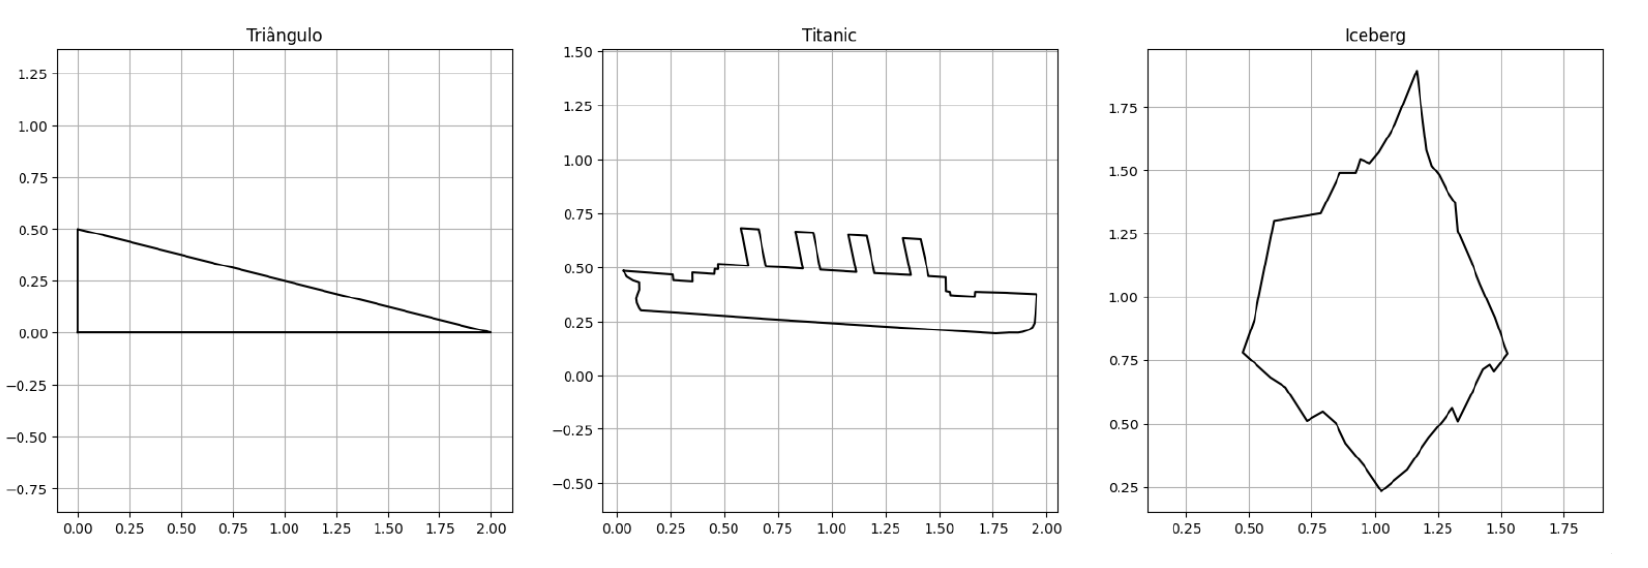
\includegraphics[width=0.9\textwidth]{objetos.png}
        \caption{Representação gráfica dos objetos}
        \label{fig:objetos}
    \end{figure}

    \begin{table}[H]
        \centering
        \begin{tabular}{cc} \\

            
            \hline
            Objeto & Densidade \\

            \hline
            Triângulo & 500.0 \\
            Iceberg & 917.0 \\
            Navio & 400.0 \\
            Água & 1000.0 \\

            \hline
        \end{tabular}
        \caption{Densidades dos objetos e da água}
        \label{table:prop}
    \end{table}

    \subsection{Grandezas e forças}
    Os desenvolvimentos teóricos desta seção foram baseados na apresentação \cite{simeoni_mecanica_fluidos_computacional}.

    Com as simplificações acima, podemos definir quais são as forças que atuam sobre o corpo. Considerando que o objeto está sob o efeito de um campo gravitacional, sabemos que ele estará sujeito a uma força peso $W$. Como estará parcialmente ou completamente submerso em algum líquido, ele sofrerá uma força de empuxo $E$ e um torque $\tau$, relacionados com a aplicação da pressão hidrostática na superfície do corpo.

    A força peso de um corpo $\Omega$ depende apenas das características geométricas e físicas do objeto, sendo dada por $W(\Omega) = - V(\Omega) \rho g$ quando a densidade do objeto é constante para todos os pontos de $\Omega$. Aqui, $V(\Omega)$ é o volume do objeto, $\rho$ é sua densidade e $g$ é a aceleração gravitacional.

    Considere agora $y_s$ a altura da superfície livre do líquido e $\rho_L$ a densidade do líquido. Definimos a pressão hidrostática no ponto $\vec{x} = (x,y)$ por:
    \[
        p(\vec{x}) = p(x,y) = \begin{cases}
            0, \text{ se } y \ge y_s \\
            \rho_L g (y_s - y), \text{ se } y \le y_s
        \end{cases}
    \]
     
    Se representarmos a posição do corpo por por um ângulo de rotação $\theta$ e por uma altura $b_2$ a partir de uma posição de referência. O empuxo é dado por:
    \[
        E(\theta, b_2, \Omega) = \oint_{\partial \Omega (\theta, b_2)} -p(\vec{x})(\check{n} \cdot \check{e_2}) ds
    \]
    Onde $\check{e_2}$ é o vetor unitário da base canônica na direção do eixo $y$, $\check{n} = (n_1, n_2)$ é a normal unitária apontando para fora do objeto. Note que para os pontos de $\partial \Omega$ acima da superfície livre, a pressão é nula, logo, eles não contribuem para o valor final da integral. Com isso, definimos $S^-(\theta, b_2) = \{(x,y) \in \partial \Omega (\theta, b_2) : y \le y_s\}$ e $S^+(\theta, b_2) = \{(x,y) \in \partial \Omega (\theta, b_2) : y > y_s \}$. Temos que $S^- \cap S^+ = \emptyset$ e $S^- \cup S^+ = \partial \Omega$. O ponto interessante é que
    \begin{equation}
        E(\theta, b_2, \Omega) = \int_{S^- (\theta, b_2)} -p(\vec{x})(\check{n} \cdot \check{e_2}) ds
        \label{eq:empuxo}
    \end{equation}
    

    Por fim, para o torque, notemos que apenas a terceira componente terá valor não nulo, pois nossos pontos estão no $\mathbb{R}^2$, logo, calculamos o torque por:
    \[
        \vec{\tau}(\theta, b_2, \Omega) = \oint_{\partial \Omega (\theta, b_2)} (\vec{x} - \vec{c}) \times (-p(\vec{x}) \check{n}) ds \implies 
    \]
    \begin{equation}
        \implies \tau(\theta, b_2, \Omega) = \vec{\tau}(\theta, b_2, \Omega) \cdot \check{e}_3 = \rho_L g \int_{S^-} y[(x - c_1)n_2 - (y-c_2)n_1] ds
    \label{eq:torque}
    \end{equation}
    Em que $\vec{c} = (c_1, c_2)$ é a posição do centro de massa do corpo.


    Dessa forma, escrevemos o balanço de forças:
    \begin{equation}
        \label{eq:forças}
        \begin{cases}
            F_x = 0 \\
            F_y = E + W \\
            F_r = \tau
        \end{cases}
    \end{equation}

    Em que $F_x$ e $F_y$ são as resultantes das forças no eixos $x$ e $y$ respectivamente e $F_r$ é a resultante da força de rotação. Definiremos $F_1(\theta, b_2) = F_y$ e $F_2(\theta, b_2) = F_r$.

    \subsubsection{Volume, centro de massa e momento de inércia}
    O empuxo e o torque foram dados em função do volume e do centro de massa de um objeto genérico, porém ainda não foi apresentada uma forma de calculá-los. Definimos assim o volume:
    \begin{equation}
        V(\Omega) = \int_\Omega dV = \frac{1}{2} \int_{\partial \Omega} \vec{x} \cdot \check{n} ds
        \label{eq:volume}
    \end{equation}
    A segunda igualdade se deve ao fato de que $1 = \frac{1}{2} \nabla \cdot \vec{x}$ e à aplicação do teorema da divergência. Se a densidade do objeto é constante, segue diretamente que a massa é dada por $m(\Omega) = \rho V$

    Já o centro de massa, no caso de densidade constante, é dado por:
    \begin{equation}
        \vec{c} = \frac{1}{V} \int_\Omega \vec{x} dV = \frac{1}{3V} \oint_{\partial \Omega} (\vec{x} \cdot \check{n})\vec{x} ds
        \label{eq:cm}
    \end{equation}
    A demonstração da segunda igualdade é omitida, pois foge do escopo deste trabalho.

    Nada foi comentado ainda sobre o momento de inércia, porém o seu cálculo será útil na seção \ref{sec:din}. Temos a fórmula:
    \[
        I = \frac{\rho}{3} \oint_{\partial \Omega} \left[ (x-c_1)^3 n_1 + (y-c_2)^3 n_2 \right] ds
    \]

    \subsection{Métodos numéricos}
    A partir do desenvolvimento teórico da seção anterior, foi possível encontrar as expressões \ref{eq:empuxo}, \ref{eq:torque}, \ref{eq:forças}, \ref{eq:volume} e \ref{eq:cm}, todas em função de uma integral no contorno do objeto. Para corpos com fronteira descrita por curvas arbitrárias, calcular essas integrais demandaria um trabalho extensivo. Dessa forma, podemos limitar os objetos àqueles descritos por apenas segmentos de retas.

    Seja $\Omega$ como acima e $\{ l_i \}^n_{i=1}$ o conjunto de segmentos de reta tal que $\partial \Omega = \bigcup_{i=1}^n l_i$. Seja $f$ uma função que iremos integrar no contorno. Logo:
    \begin{equation}
        \int_{\partial \Omega} f(\vec{x}) ds = \sum_{i=1}^{n} \int_{l_i} f(\vec{x}) ds
    \end{equation}
    Reduzimos o problema a calcular integrais em retas. Para fazer esse procedimento numericamente, parametrizamos cada reta no intervalo $[-1,1]$ e aplicamos a quadratura de Gauss-Legendre, que integra exatamente polinômios de grau até no máximo $2m-1$, em que $m$ é o número de pontos usados na quadratura. Note que as funções que iremos integrar são polinômios de grau no máximo 2, logo basta usar 2 ou 3 pontos na quadratura. 

    \subsubsection{Parametrização das retas}
    Dada uma reta em $\mathbb{R}$ com pontos inicial e final $\vec{x}^i = (x^i, y^i)$ e $\vec{x}^f = (x^f, y^f)$ respectivamente, queremos um mapeamento afim do intervalo $[-1,1]$ para o segmento. Seja $T_{k}:[-1,1] \to \mathbb{R}^2$ esse mapeamento para a reta $l_k$. Temos:
    \[
        \begin{cases}
            T_k(\xi) = \alpha \xi + \beta, \xi \in [-1,1] \\
            T_k(-1) = \vec{x}^i \\
            T_k(1) = \vec{x}^f
        \end{cases}
    \] 
    Essas condições definem um sistema que tem solução única dada por
    \[
        T_k(\xi) = \frac{1-\xi}{2}\vec{x}^i + \frac{1 + \xi}{2} \vec{x}^f
    \]

    Por fim, como precisaremos integrar em $\xi$:
    \[
        ds = \Vert T_k'(\xi)\Vert d \xi = \left\Vert \frac{\vec{x}^f - \vec{x}^i}{2} \right\Vert d \xi
    \]

    \subsubsection{Aplicação da quadratura}
    Com a parametrização, podemos agora escrever:
    \begin{equation}
        \int_{\partial \Omega} f(\vec{x}) ds = \sum_{k=1}^{n} \int_{l_k} f(\vec{x}) ds = \sum_{k=1}^{n} \int^1_{-1} f(T_k(\xi)) \left\Vert \frac{\vec{x}^f - \vec{x}^i}{2} \right\Vert d \xi
        \label{eq:param}
    \end{equation}

    Lembremos que uma regra de quadratura é tal que 
    \[
        \int_{a}^{b} f(x) dx \approx \sum_{j=1}^{m} A_j f(x_j)
    \]
    em que os pesos $A_j$ e os pontos de quadratura $x_j$ dependem da regra que estamos usando. Aplicando a quadratura de Gauss-Legendre, podemos aproximar a integral:
    \begin{equation}
        \sum_{k=1}^{n} \int^1_{-1} f(T_k(\xi)) \left\Vert \frac{\vec{x}^f - \vec{x}^i}{2} \right\Vert d \xi \approx \sum_{k=1}^{n} \sum_{j=1}^{m} A_j f(T_k(\xi_j)) \left\Vert \frac{\vec{x}^f - \vec{x}^i}{2} \right\Vert
        \label{eq:quad}
    \end{equation}

    Isso nos dá um procedimento computável para as integrais \ref{eq:empuxo}, \ref{eq:torque}, \ref{eq:forças}, \ref{eq:volume} e \ref{eq:cm}.

    \subsubsection{Segmentação de retas}
    Para calcular o empuxo e o torque, note que a integral é sobre $S^-$, pois a pressão é nula para pontos acima da superfície livre do líquido. Logo, se algum segmento de reta estiver parcialmente submerso, precisamos dividir ele entre a parte acima e abaixo de $y_s$. Este problema pode ser formulado como encontrar $\xi_s$ tal que $T_k(\xi_s) = y_s$. Encontrado $\xi_s$, calculamos $x_s$ e temos uma nova reta formada pelo ponto submerso da reta e $(x_s, y_s)$.
    \[
        T_k(\xi_s) = y_s \implies \frac{1-\xi}{2}\vec{x}^i + \frac{1 + \xi}{2} \vec{x}^f = y_s \implies \xi_s = \frac{2y_s - (y^f + y^i)}{y^f - y^i}
    \]
    E, por fim, $(x_s, y_s) = T_k(\xi_s)$
    \subsection{Implementação}
    Os corpos são formados por segmentos de retas e sofrerão ação de transformações rígidas. Dessa forma, um objeto foi representado da seguinte maneira:
    \[
        \begin{bmatrix}
            x^i_1 & x^i_2 & \dots & x^i_n \\
            y^i_1 & y^i_2 & \dots & y^i_n \\
            1     & 1     & \dots & 1 \\
            x^f_1 & x^f_2 & \dots & x^f_n \\
            y^f_1 & y^f_2 & \dots & y^f_n \\
            1     & 1     & \dots & 1 \\
        \end{bmatrix} = \begin{bmatrix}
            \vec{X}^i \\
            \vec{1} \\
            \vec{X}^f \\
            \vec{1}
        \end{bmatrix}
    \]
    Ou seja, cada coluna representa uma reta: as duas primeiras entradas correspondem ao ponto inicial e as entradas 4 e 5 representam as coordenadas do ponto final. Note que depois das coordenadas, temos um vetor de uns. Isso representa uma coordenada homogênea, de forma a facilitar as transformações rígidas, reduzindo-as a um produto matriz-vetor. 

    De fato, se $B$ é uma transformação rígida, ela é uma composição de translações $T$ e rotações $R$, que, quando introduzimos uma coordenada homogênea, podem ser representadas por:
    \begin{align}
        R = \begin{bmatrix}
            \cos(\theta) & -\sin(\theta) & 0 \\
            \sin(\theta) & \cos(\theta) & 0 \\
            0 & 0 & 1
        \end{bmatrix} && T = \begin{bmatrix}
            1 & 0 & t_x \\
            0 & 1 & t_y \\
            0 & 0 & 1 
        \end{bmatrix} \notag
    \end{align}
    Logo, $B$ tem representação matricial e basta fazermos $B (x^i, y^i, 1)$ e $B (x^f, y^f, 1)$ para fazer a transformação rígida em cada reta. Ou seja, aplicar a transformação rígida ao objeto inteiro pode ser escrito como o produto abaixo seguido de uma concatenação vertical de matrizes.
    \begin{align}
        B \begin{bmatrix}
            \vec{X}^i \\
            \vec{1}
        \end{bmatrix} && B \begin{bmatrix}
            \vec{X}^f \\
            \vec{1}
        \end{bmatrix}
    \end{align}
 
    Essa estrutura facilita também a parametrização. Dado $\xi$, podemos encontrar os pontos dados pela parametrização de todas as retas do objeto por $\xi$:
    \[
        T(\xi) = \frac{1 - \xi}{2} \vec{X}^i + \frac{1 + \xi}{2}\vec{X}^f
    \]
    Para a integração numérica, considere $g(\vec{x})$ os argumentos das integrais \ref{eq:empuxo}, \ref{eq:torque}, \ref{eq:forças}, \ref{eq:volume} e \ref{eq:cm}. Fazemos
    \[
        G= \begin{bmatrix}
            g_T(T(\xi_1)) \\
            \dots \\
            g_T(T(\xi_m))
        \end{bmatrix}
    \] 
    com $\xi_k$ os pontos de quadratura. A $g$, normalmente definida $\mathbb{R}^2 \mapsto \mathbb{R}$ ($\mathbb{R}^2$ no caso do centro de massa), é modificada para $g_T$, de forma que os inputs pertencem a $\mathbb{R}^{2 \times n}$ e o output está em $\mathbb{R}^{1 \times n}$ e é multiplicado, componente a componente, pelo vetor
    \[
        \left\Vert \frac{\vec{X}^f - \vec{X}^i}{2} \right\Vert_{vertical}
    \]
    em que $||\cdot||_{vertical}$ toma a norma das colunas.
    Podemos também representar os pesos de quadratura por um vetor $A=(A_1, \dots, A_m)^\top$. Logo $A^\top G$ nos dá um vetor horizontal contendo a integração numérica em cada linha. Por fim, a integral no corpo é dada por
    \[
        Int = \sum_{j=1}^{n} (A^\top G)_{1j}
    \]

    Para os casos que devemos integrar em $S^-$, fazemos uma segmentação como já descrita, porém tomando como entrada a matriz do corpo e retornando uma matriz com a mesma estrutura contendo apenas as partes dos segmentos submersas.

    \subsection{Encontrando pontos de equilíbrio}
    Pontos de equilíbrio ocorrem quando as forças no corpo são nulas, ou seja
    \begin{equation}
        \begin{cases}
            F_1(\theta, b_2) = 0 \\
            F_2(\theta, b_2) = 0
        \end{cases}
        \label{eq:equilibrium}
    \end{equation}
    Note que isso é um sistema de eequações não lineares em $\theta$ e $b_2$. Podemos então aplicar o método de Newton-Raphson para encontrar as raízes desse sistema. Seja $F(\vec{u}) = \begin{bmatrix}
        F_1(\vec{u}) \\
        F_2(\vec{u})
    \end{bmatrix}$ e $J_F(\vec{u})$ a matriz jacobiana de $F$, com $\vec{u} = (u_1, u_2) = (\theta, b_2)$. Uma iteração do método de Newton é dada por:
    \begin{equation}
        \begin{cases}
            J_F(\vec{u}^k) \vec{\delta}^k = -F(\vec{u}^k) \\
            \vec{u}^{k+1} = \vec{u}^k + \vec{\delta}^k
        \end{cases}
        \label{eq:Newton}
    \end{equation}
    Tomamos $\vec{u}^0$ próximo de algum ponto de equilíbrio paramos a iteração quando $\\||vec{\delta}^k||, ||F(\vec{u}^k)|| \le \varepsilon$, sendo $\varepsilon$ uma tolerância, aqui tomada como $1e-11$.

    Porém, calcular $J_F$ analiticamente não é trivial, dado que $F$ não tem uma forma explícita, dificultando encontrar as derivadas. Usamos então diferenças finitas para aproximar essas derivadas e, consequentemente a Jacobiana. Logo, temos:
    \begin{equation}
        \frac{\partial F_i}{\partial u_j}(\vec{u}) \approx \frac{F_i(\vec{u} + \Delta u_j) - F_i(\vec{u} - \Delta u_j)}{2 \Delta u_j}
        \label{eq:fin_dif}
    \end{equation}
    em que $\Delta u_j = \Delta\check{e}_j$ com $\Delta$ um escalar pequeno (foi usado $\Delta = 1e-4$). Essa aproximação tem erro na ordem de $O(\Delta^2)$.

    \subsubsection{Velocidade de convergência do método}
    Definimos a ordem de convergência de um método numérico (\cite{franco_calculo_numerico}) para encontrar raízes de sistemas de equações por: $p$ tal que $\exists c > 0$ e:
    \[
        \lim_{k \to \infty} \frac{|e_{k+1}|}{|e_k|^p} = c
    \]

    com $e_k = x_k - \bar{x}$ e $\bar{x}$ solução da equação. $p$ pode ser estimado por 
    \[
        p_k \approx \frac{\ln\left( \frac{e_{k+1}}{e_k} \right)}{\ln\left( \frac{e_k}{e_{k-1}} \right)}
    \]

    Tomando $\bar{x}$ como o último valor encontrado pelo método de Newton $\vec{u}^n$, podemos calcular a ordem média de convergência do método por 
    \[
        p_{mean} = \frac{1}{n}\sum_{k=1}^{n-1} p_k
    \]


    \subsection{Dinâmica}
    \label{sec:din}
    Pela segunda lei de Newton, sabemos que:
    \[
        m \frac{d^2b_2}{dt^2} = F_y = F_1
    \]
    e
    \[
        I \frac{d^2 \theta}{dt^2} = F_r = F_2
    \]
    É natural que exista alguma força dissipativa decorrente do atrito do objeto com o líquido, logo, podemos escrever:
    \begin{equation}
        \begin{cases}
            m \frac{d^2b_2}{dt^2} = F_1 - \gamma_1 V \frac{db_2}{dt} \\
            I \frac{d^2 \theta}{dt^2} = F_2 - \gamma_2 I \frac{d\theta}{dt}
        \end{cases}
    \end{equation}
    Com $\gamma_1$ e $\gamma_2$ coeficientes de amortecimento para as forças verticais e de rotação respectivamente. Essas duas eequações regem o movimento do corpo. Para utilizá-las numericamente, podemos transformá-las em um sistema de eequações diferenciais do primeiro grau e então aplicar algum método para Problemas de Valor Inicial (PVI). Seja
    \[
        u(t) = \begin{bmatrix}
            b_2(t) \\
            b_2'(t) \\
            \theta(t) \\
            \theta '(t)
        \end{bmatrix} = \begin{bmatrix}
            u_0 \\ u_1 \\ u_2 \\ u_3
        \end{bmatrix}
    \]

    Logo
    \[
        u'(t) = f(u(t)) = \begin{bmatrix}
            u_1 \\
            \frac{1}{m} (F_1(u_2, u_0) - \gamma_1 V u_1) \\
            u_3 \\
            \frac{1}{I}(F_2(u_2, u_0) - \gamma_2 I u_3)
        \end{bmatrix}
    \]
    Com uma condição inicial $u^0$. Foram escolhidos 3 valores para $\gamma_1$ e $\gamma_2$, resultando em 9 testes por objeto. Defina $c_1 = \frac{\gamma_1 V}{m} = \frac{\gamma_1}{\rho}$ e $c_2 = \gamma_2$. Para os dois coeficientes, foram escolhidos os valores tal que:
    \begin{table}[H]
        \centering
        \begin{tabular}{cc} \\

            
            \hline
            $c_1$ & $c_2$ \\

            \hline
            $\ll 1$ & 0.5 \\
            1.0 & 1.0 \\
            10.0 & 10.0 \\

            \hline
        \end{tabular}
        \caption{Valores usados para $c_1$ e $c_2$}
    \end{table}

    Neste trabalho, foi aplicado o método Runge-Kutta de quarta ordem (RK4 clássico) para a solução do PVI.













    \section{Resultados}
    Para todos os objetos, a posição de referência $(\theta, b_2) = (0,0)$ é quando o centro de massa está na origem. Além disso, a superfície da água foi escolhida como $y_s = 0.0$ para todos os casos.

    Os PVIs foram calculados usando um passo de tempo $h = 0.03$, tempo final $t_f = 40.0$, tempo inicial $t_0 = 0.0$, e condição inicial $u^0 = (0,0,0,0)$.


    \subsection{Consistência do código}
    Para verificar a consistência dos códigos e métodos, foi aplicado o método da solução manufaturada. Foi criado um objeto, e foram calculados analiticamente o seu volume, peso, centro de massa e empuxo em duas situações diferentes (Totalmente submerso e parcialmente submerso). O corpo consiste no barco da figura \ref{fig:man_sol} com $\rho = 0.5$ e densidade do líquido $\rho_L = 1.0$.
    \begin{figure}[H]
        \centering
        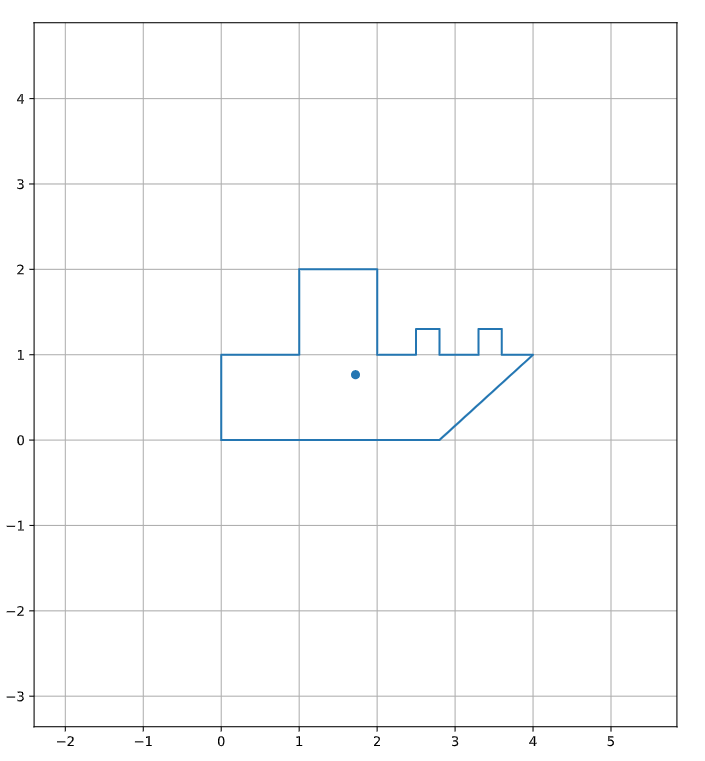
\includegraphics[width=0.5\textwidth]{man_sol.png}
        \caption{Objeto da solução manufaturada}
        \label{fig:man_sol}
    \end{figure}
    Os resultados podem ser vistos na Tabela \ref{table:man_sol}
    \begin{table}[H]
        \centering
        \begin{tabular}{cccc} \\

            
            \hline
            Grandeza & Valor analítico & Valor calculado & Erro absoluto \\

            \hline
            Volume & 4.5800 & 4.5800 & 0.0000 \\
            Centro de massa & (1.7225, 0.7657) & (1.7225, 0.7657) & (0.0000, 0.0000) \\
            Empuxo (Totalmente sub.) & 44.9298 & 44.9298 & 0.0000 \\
            Empuxo (Parcialmente sub.) & 33.354 & 33.354 & 0.0000 \\

            \hline
        \end{tabular}
        \caption{Comparação dos resultados analíticos e calculados computacionalmente}
        \label{table:man_sol}
    \end{table}

    Ademais, foi verificada a convergência dos cálculos em função do número de retas na segmentação de um círculo com raio $r= 1.0$, $\rho = 0.5$ e $\rho_L=1.0$. Os erros cometidos nos cálculos podem ser vistos nas tabelas \ref{table:conv_circle1} e \ref{table:conv_circle2}.
    \begin{table}[H]
        \centering
        \begin{tabular}{rrrr} \\

            
            \hline
 \\
\hline
            Número de segmentos &      Volume &   Centro de massa &        Peso \\

            \hline
                                4 &     1.14159 &       3.14018e-16 &      11.199 \\
                                8 &    0.313166 &                 0 &     3.07215 \\
                                16 &   0.0801252 &                 0 &    0.786028 \\
                                32 &   0.0201475 &                 0 &    0.197647 \\
                                64 &  0.00504416 &       4.96507e-16 &   0.0494832 \\
                            128 &   0.0012615 &       2.22045e-16 &   0.0123753 \\
                            256 & 0.000315403 &       3.14018e-16 &   0.0030941 \\
                            512 & 7.88524e-05 &       2.22045e-16 & 0.000773542 \\
                            1024 & 1.97132e-05 &                 0 & 0.000193387 \\
                            2048 & 4.92831e-06 &       3.14018e-16 & 4.83467e-05 \\
                            4096 & 1.23208e-06 &       3.14018e-16 & 1.20867e-05 \\
                            8192 &  3.0802e-07 &       2.22045e-16 & 3.02167e-06 \\
                            16384 & 7.70049e-08 &                 0 & 7.55418e-07 \\

            \hline
        \end{tabular}
        \caption{Erros numéricos cometidos ao aproximar um círculo por segmentos de reta}
        \label{table:conv_circle1}
    \end{table} 

    \begin{table}[H]
        \centering
        \begin{tabular}{rrrr} \\

            
            \hline
 \\
\hline
            Número de segmentos &      Torque &      Empuxo &   Momento de inércia \\

            \hline
                                4 &  1.9984e-15 &     5.59951 &              0.90413 \\
                                8 &  9.4369e-16 &     1.53608 &             0.294654 \\
                                16 & 2.35922e-16 &    0.393014 &            0.0789027 \\
                                32 & 2.90566e-16 &   0.0988235 &              0.02007 \\
                                64 & 2.50884e-16 &   0.0247416 &            0.0050393 \\
                            128 & 1.57074e-17 &  0.00618764 &           0.00126119 \\
                            256 & 7.53334e-17 &  0.00154705 &          0.000315384 \\
                            512 & 1.21946e-16 & 0.000386771 &          7.88513e-05 \\
                            1024 & 9.52675e-17 & 9.66934e-05 &          1.97131e-05 \\
                            2048 & 4.40118e-18 & 2.41734e-05 &          4.92831e-06 \\
                            4096 & 3.22076e-17 & 6.04335e-06 &          1.23208e-06 \\
                            8192 & 4.13283e-16 & 1.51084e-06 &           3.0802e-07 \\
                            16384 &  1.3001e-16 & 3.77709e-07 &          7.70049e-08 \\

            \hline
        \end{tabular}
        \caption{Erros numéricos cometidos ao aproximar um círculo por segmentos de reta}
        \label{table:conv_circle2}
    \end{table}

    O número de segmentos está dobrando, enquanto todas as grandezas estão diminuindo por um fator de $0.25$, indicando que a convergência em relação ao número de segmentos é de segunda ordem. Além disso, isso mostra a consistência do cálculo do torque e do momento de inércia implementados.

    \subsection{Sobre curvas de força}
    O método de Newton-Raphson possui convergência garantida apenas local, dependendo fortemente do ponto inicial para fazer a iteração. Além disso, se uma equação tem mais de uma solução, a solução encontrada também depende desse ponto inicial. 
    
    Uma das maneiras para encontrar um bom ponto inicial de forma qualitativa é mapear as forças $F_1$ e $F_2$ para $\theta \in [0, 2\pi]$ e $b_2 \in [-d, d]$, em que $d$ é a maior distância entre dois pontos do objeto. Com as funções mapeadas, basta localizar os pontos em que $F_1$ e $F_2$ são simultaneamente próximos de zero. Dessa forma, também é útil verificar as curvas de nível dessas funções.

    Outro ponto importante é que, um ponto de equilíbrio pode ser instável ou estável. Em um ponto $P$ de equilíbrio, as forças são nulas, porém podem não ser em uma vizinhança de $P$. Se, em geral (e informalmente), elas apontam para a direção oposta de $P$, então o objeto tende a sair dessa posição de equilíbrio com qualquer perturbação e chamamos o equilíbrio de instável. Caso contrário, ele é estável.

    A diferenciação de pontos de equilíbrio é importante para a variante dinâmica do problema da flutuação, pois em geral, todos os regimes estacionários obtidos pela solução do PVI serão pontos de equilíbrio estável.



    \subsection{Iceberg}
    \label{sec:ice}
    \subsubsection{Mapeamento de forças}
    \label{sec:ice_forca}
    Fazendo o mapeamento de forças para o iceberg, obtemos o plot da figura \ref{fig:iceberg_level}.
    \begin{figure}[H]
        \centering
        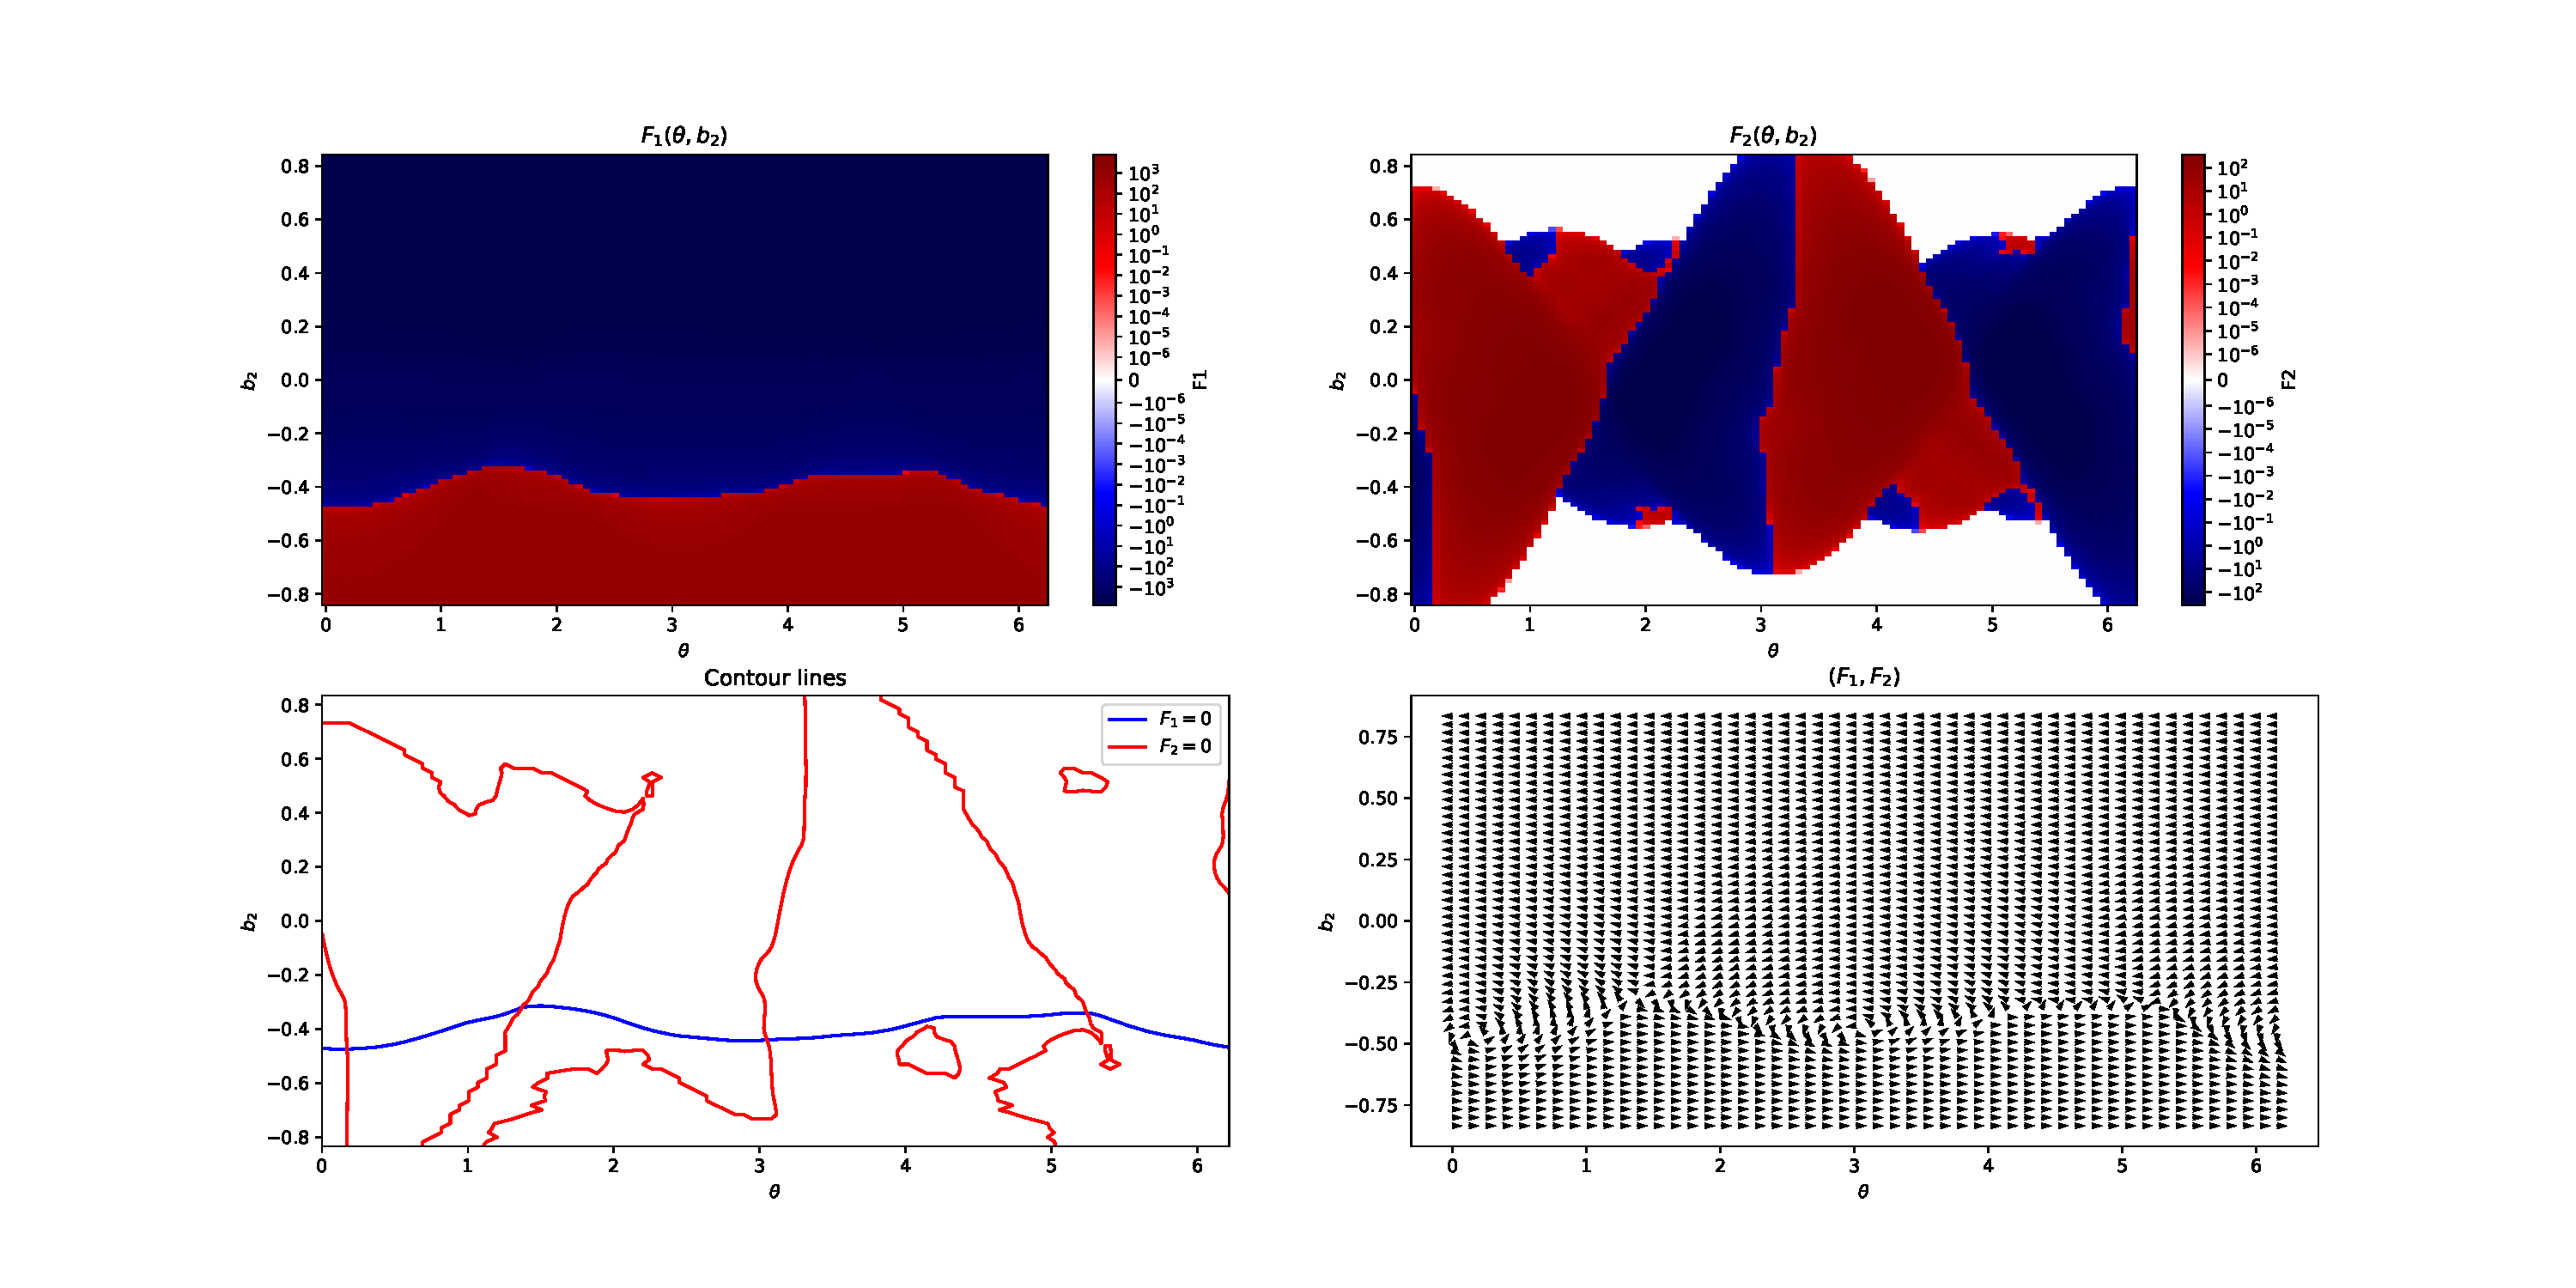
\includegraphics[width=1.0\linewidth]{iceberg/levels.pdf}
        \caption{Curvas de força do iceberg}
        \label{fig:iceberg_level}
    \end{figure}
    Verificamos 4 pontos de equilíbrio pelo plots das curvas de nível. Qualitativamente, verificamos as possíveis posições iniciais para o método de Newton:
    \begin{table}[H]
        \centering
        \begin{tabular}{ccc} \\

            
            \hline
            Índice do ponto & $\theta$ aproximado & $b_2$ aproximado \\

            \hline
            1 & 0.0 & -0.5 \\
            2 & 1.3 & -0.3 \\
            3 & 3.0 & -0.5 \\
            4 & 5.3 & -0.4 \\

            \hline
        \end{tabular}
        \caption{Aproximações dos pontos de equilíbrio do iceberg}
        \label{table:ice_approx}
    \end{table}
    Pelo plot do campo vetorial, verificamos que os pontos 1 e 3 são pontos de equilíbrio instável, pois os vetores de força apontam para fora em algo que parece uma espiral. Para os pontos 2 e 4, alguns vetores de força divergem, enquanto outros convergem para o ponto, tornando a análise sobre o equilíbrio desses pontos inconclusiva pelo gráfico.

    \subsubsection{Pontos de equilíbrio}
    Com os pontos aproximados encontrados na seção \ref{sec:ice_forca}, aplicamos o método de Newton, encontrando as posições de equilíbrio da figura \ref{fig:iceberg_equi}, também explicitados na tabela \ref{table:iceberg_equi}.

    \begin{figure}[!h]
        \centering
        \begin{subfigure}[b]{0.45\textwidth}
            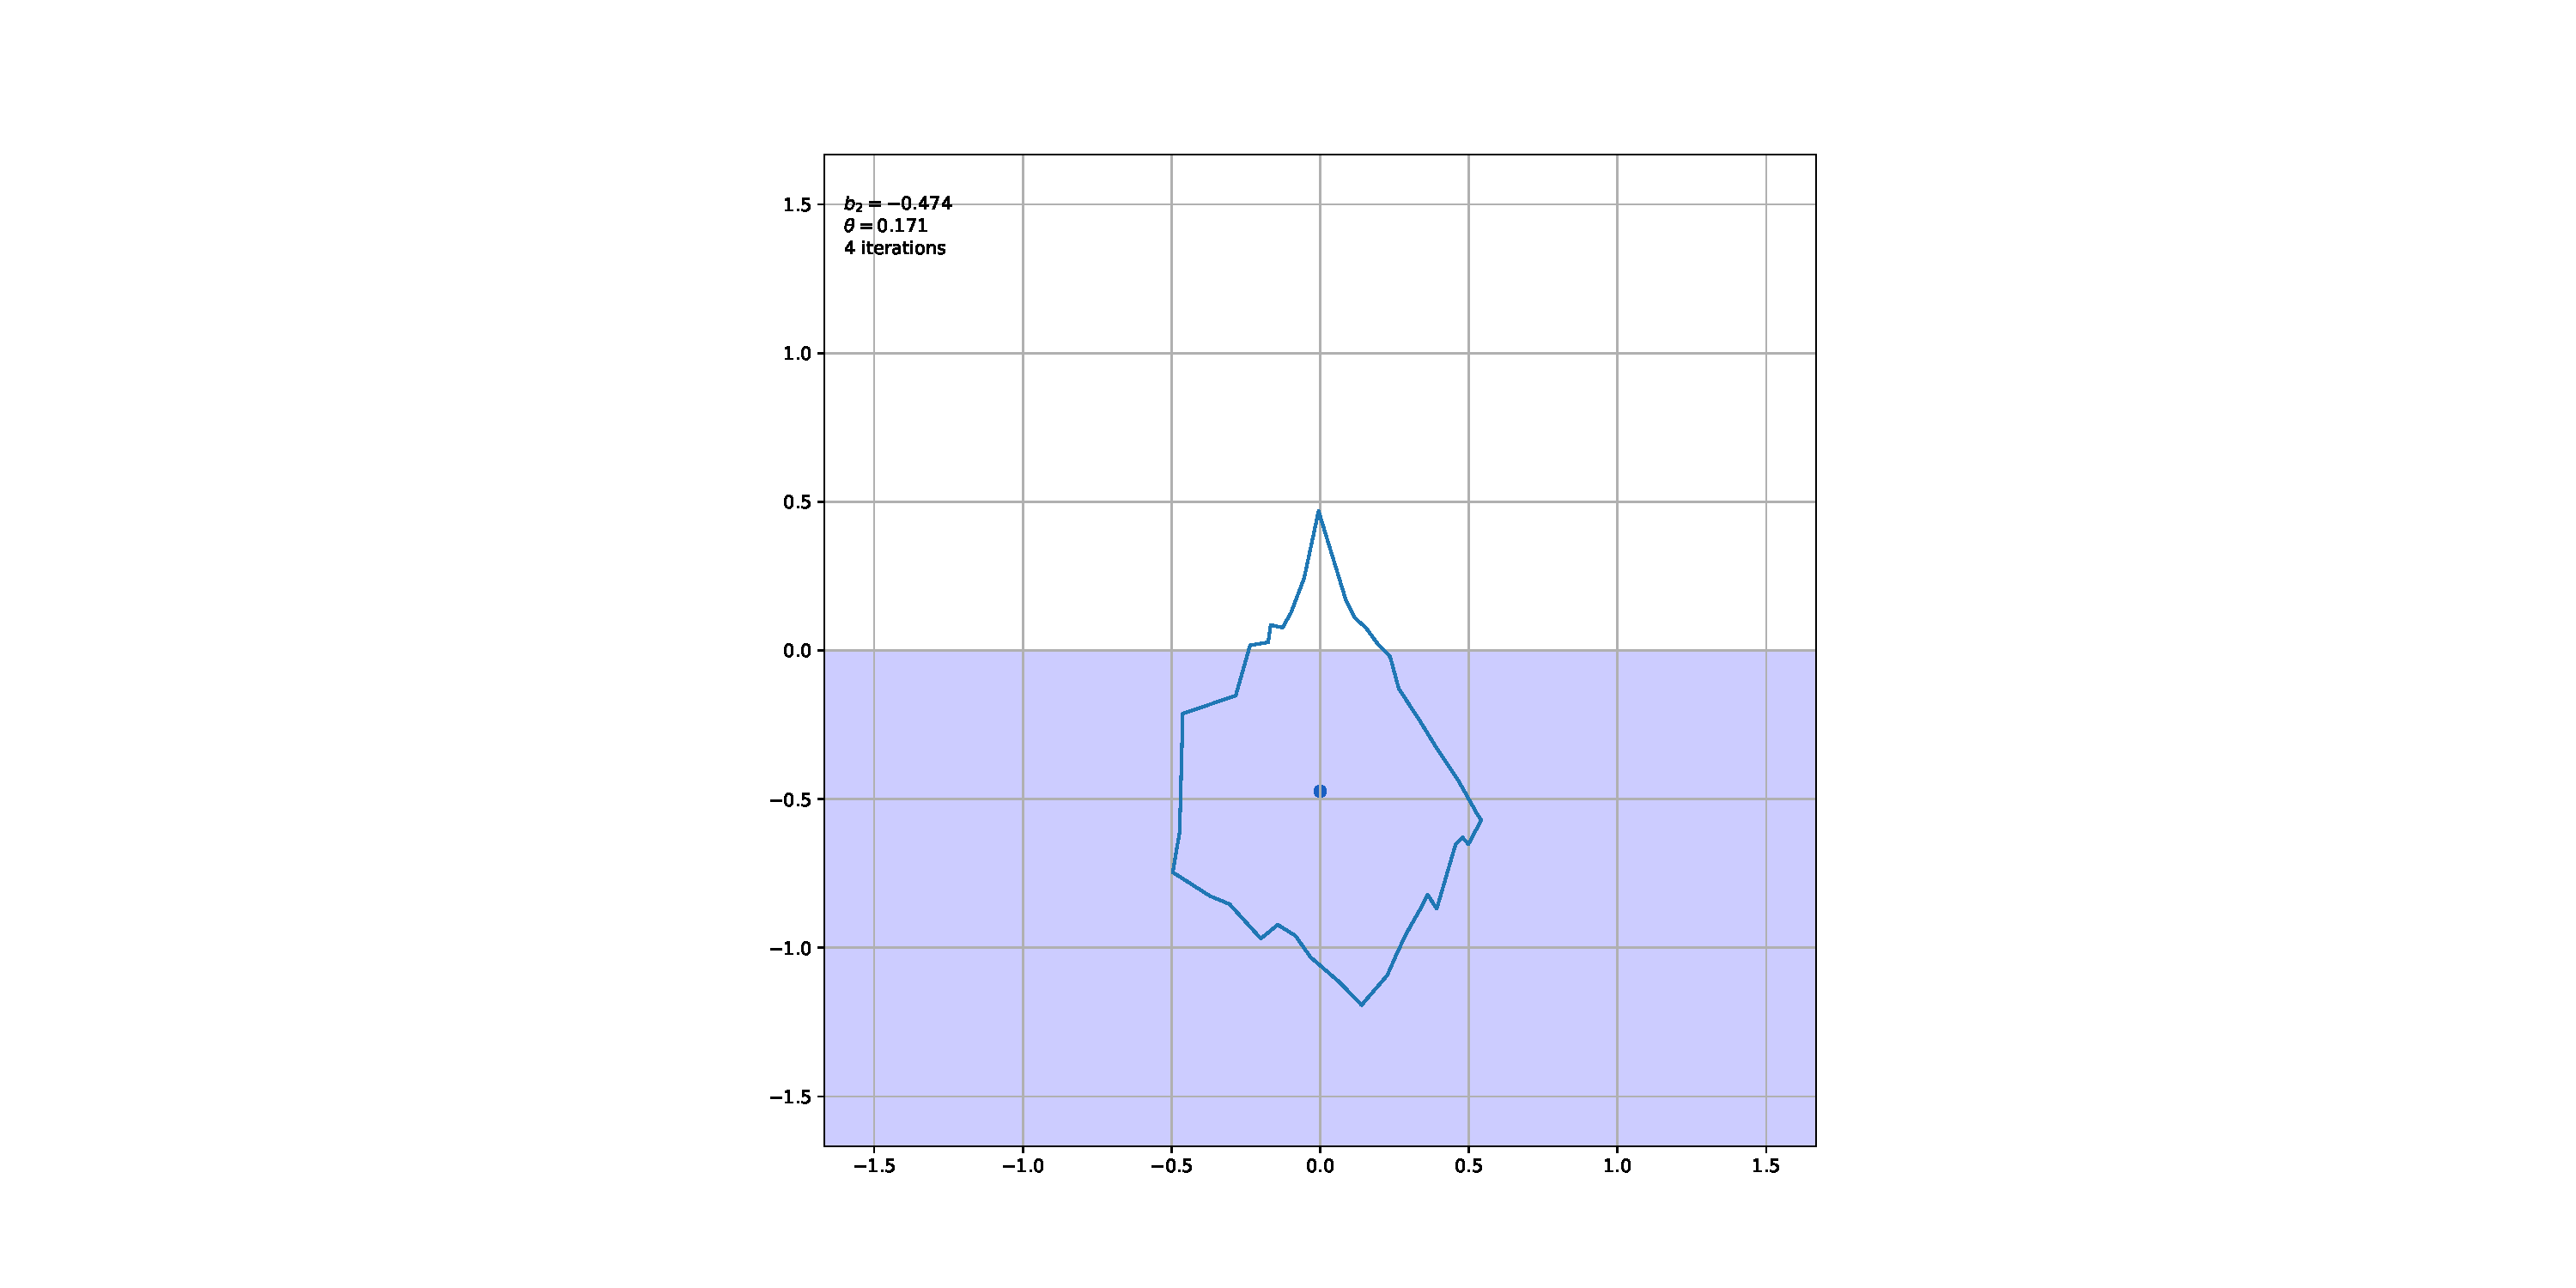
\includegraphics[width=\textwidth]{iceberg/newton_b0=-0.500_theta0=0.000.pdf}
            \caption{Partindo do ponto 1}
        \end{subfigure}
        \quad
        \begin{subfigure}[b]{0.45\textwidth}
            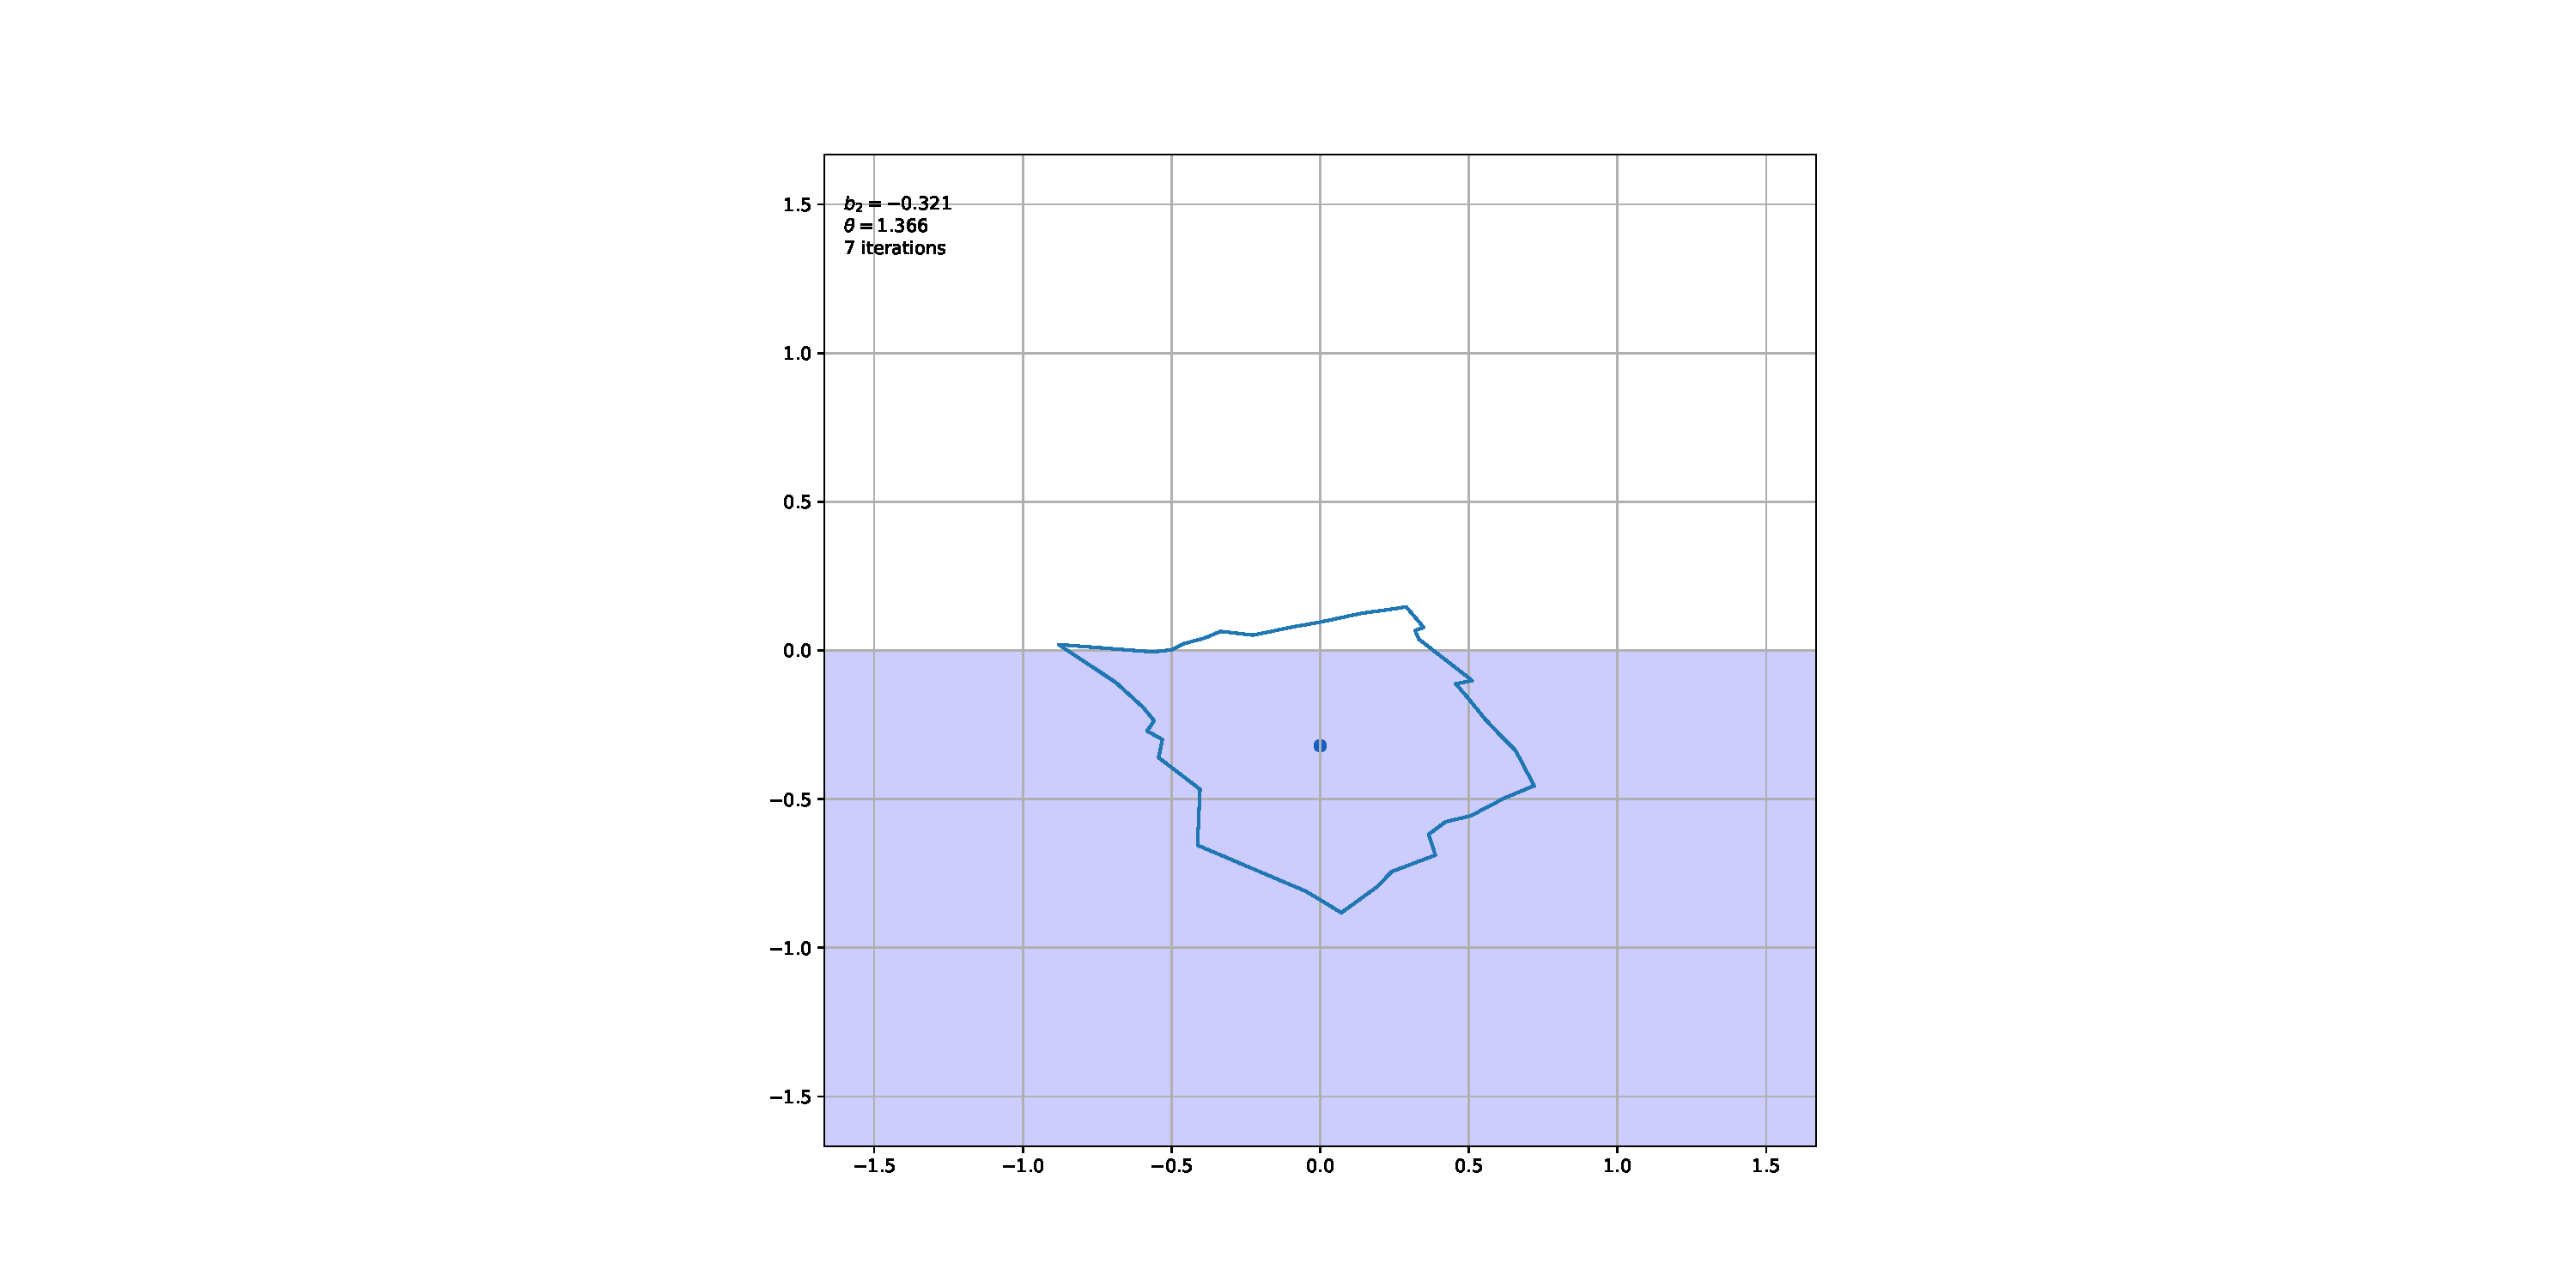
\includegraphics[width=\textwidth]{iceberg/newton_b0=-0.300_theta0=1.300.pdf}
            \caption{Partindo do ponto 2}
        \end{subfigure}
        \quad
        \begin{subfigure}[b]{0.45\textwidth}
            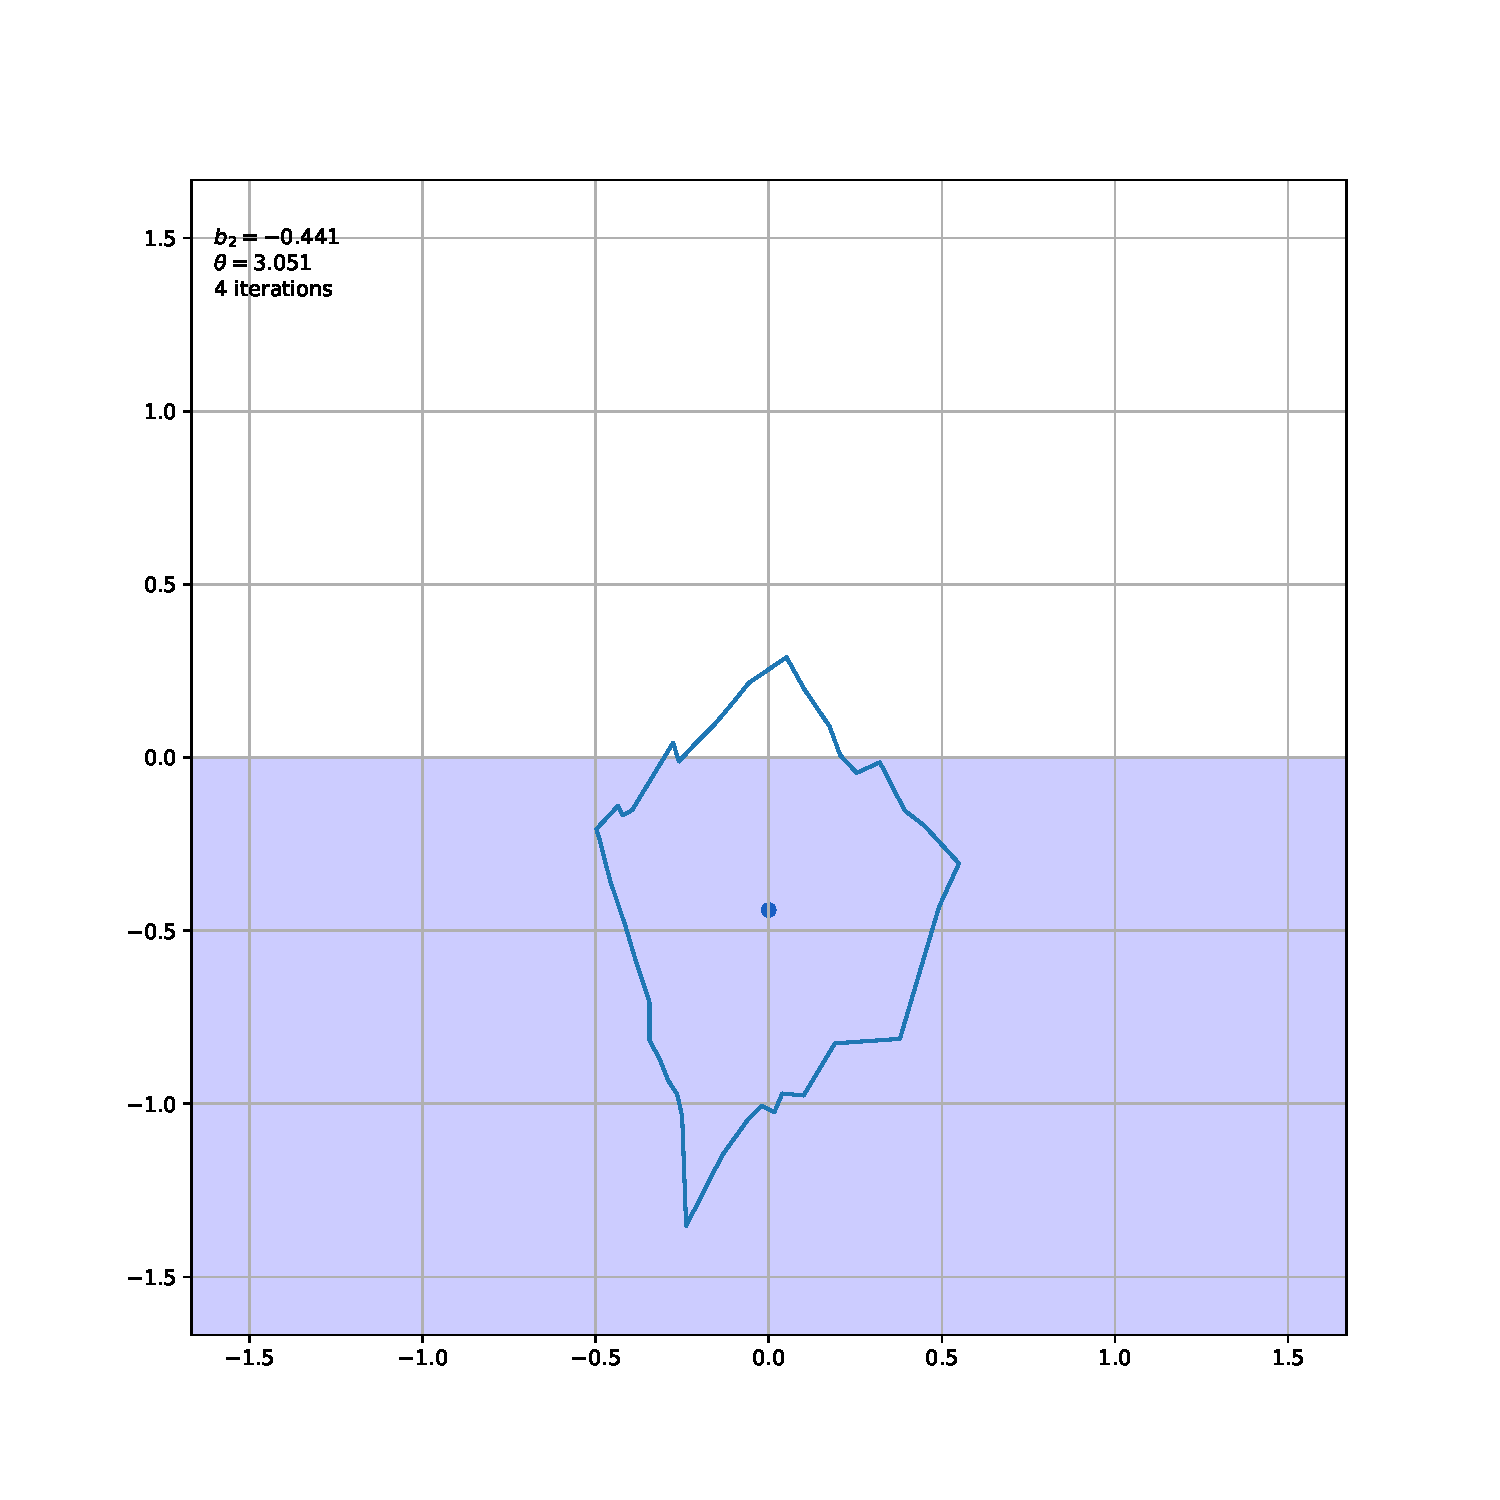
\includegraphics[width=\textwidth]{iceberg/newton_b0=-0.500_theta0=3.000.pdf}
            \caption{Partindo do ponto 3}
        \end{subfigure}
        \quad
        \begin{subfigure}[b]{0.45\textwidth}
            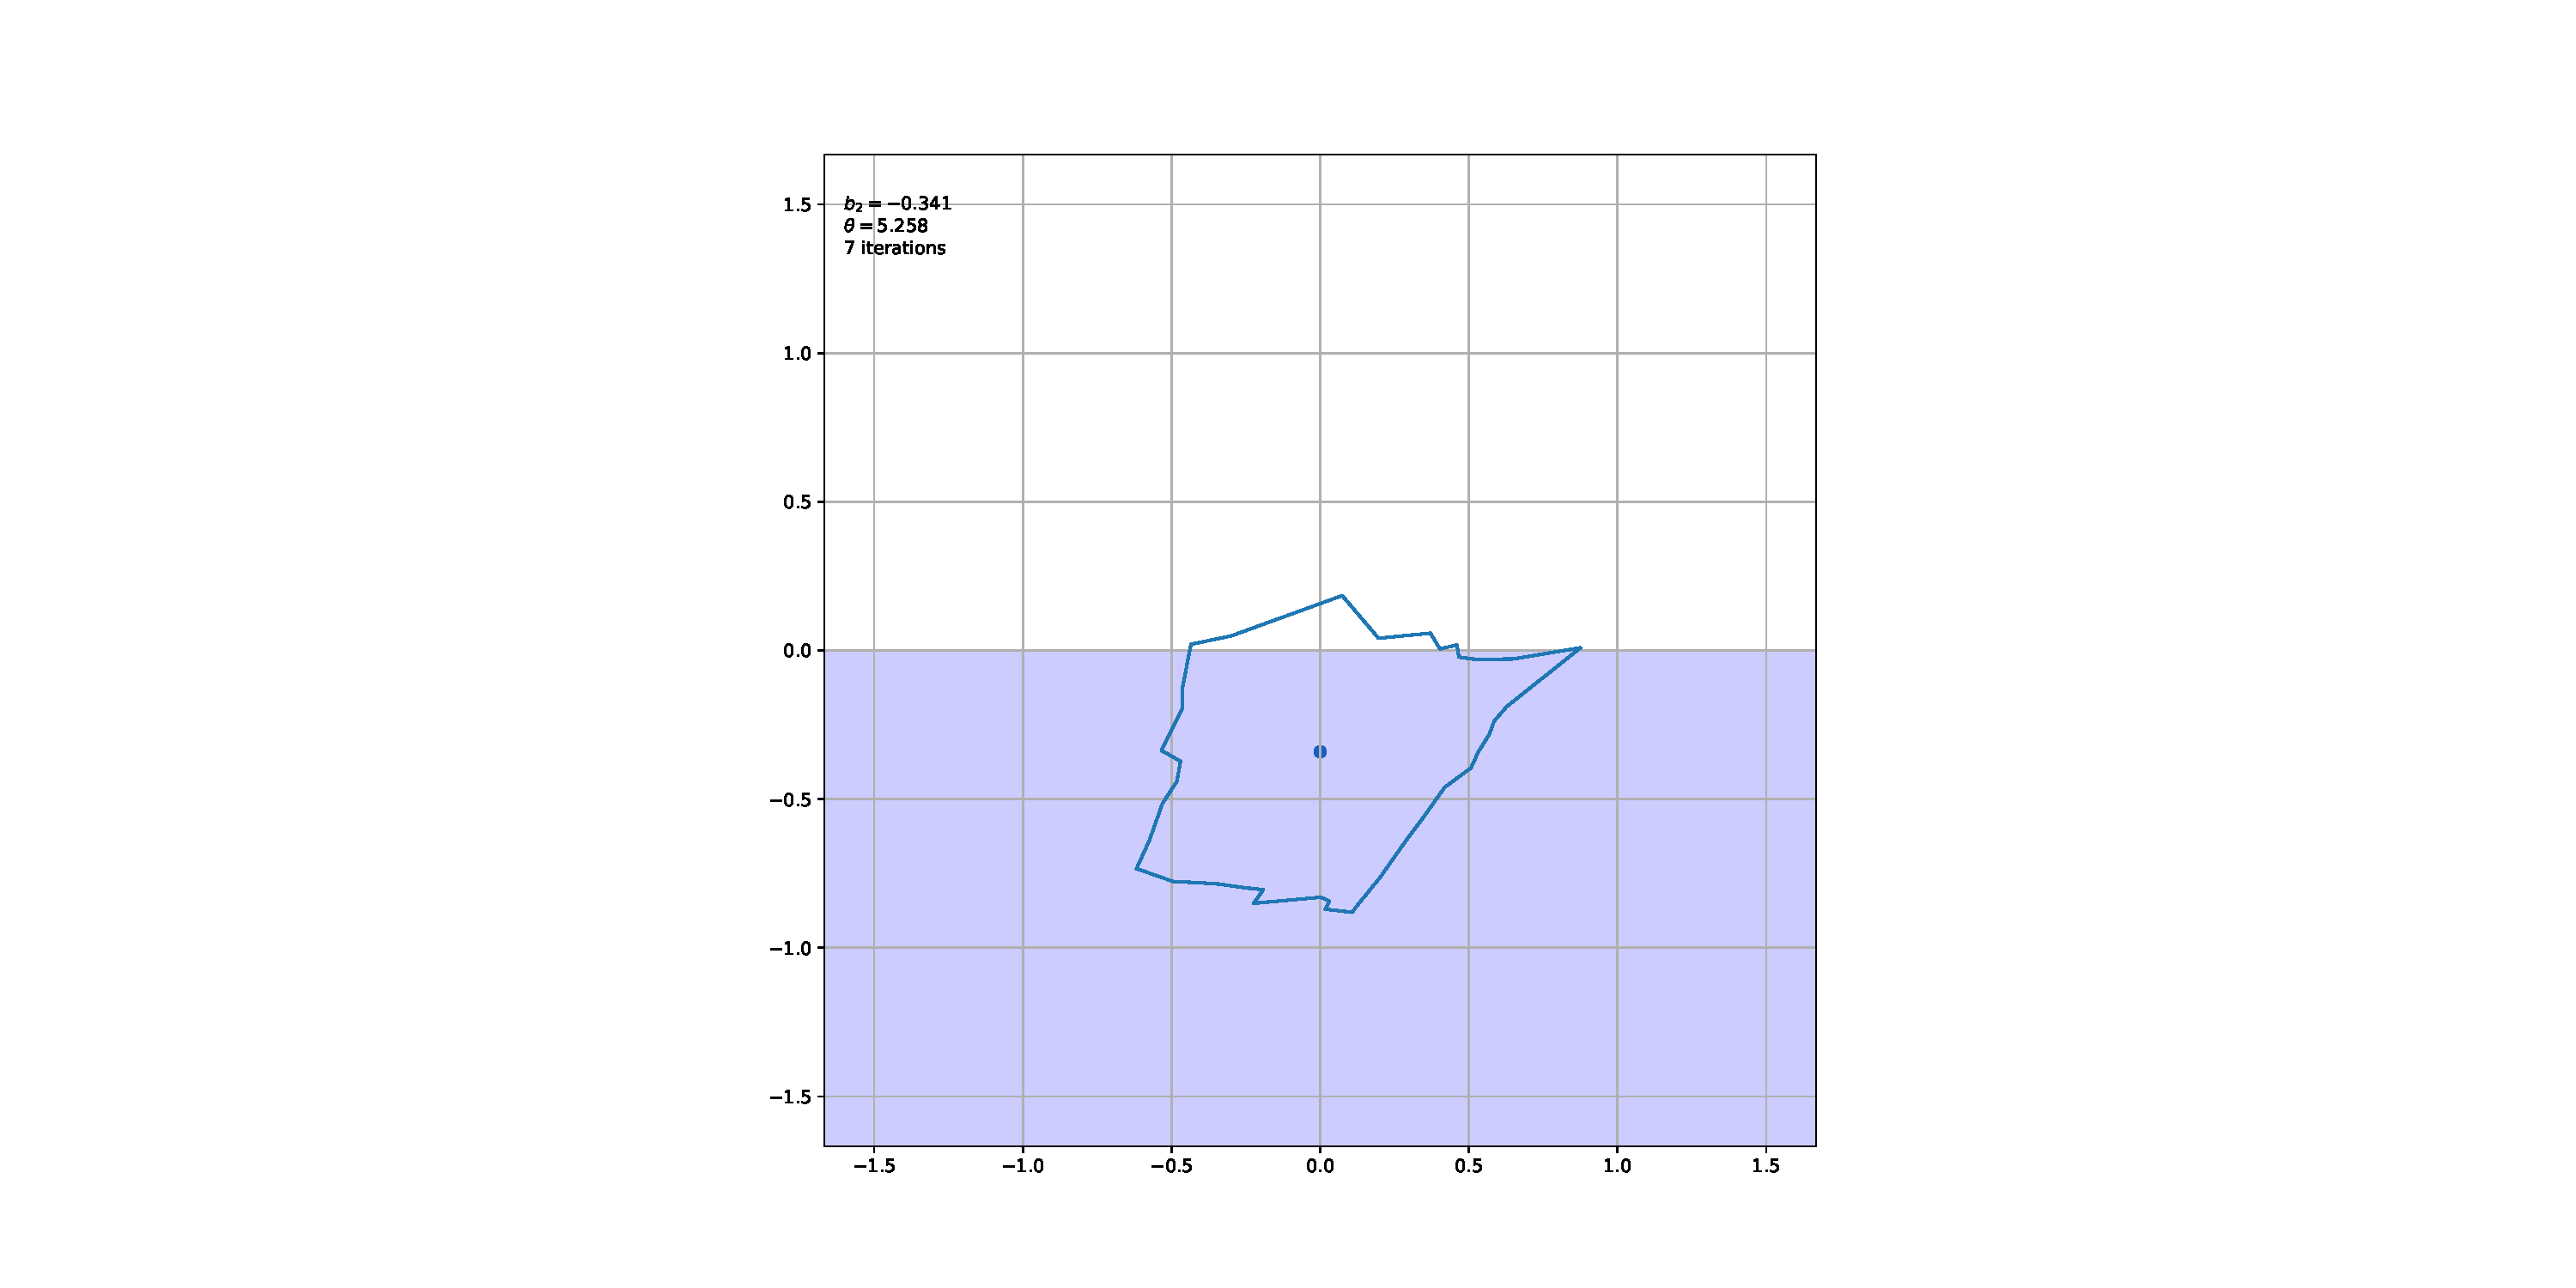
\includegraphics[width=\textwidth]{iceberg/newton_b0=-0.400_theta0=5.300.pdf}
            \caption{Partindo do ponto 4}
        \end{subfigure}

        \caption{Pontos de equilíbrio encontrados para o iceberg}
        \label{fig:iceberg_equi}
    \end{figure}

    \begin{table}[h]
        \centering
        \begin{tabular}{ccccc} \\

            
            \hline
            Índice & $\theta$ & $b_2$ & Iterações & Ordem média de convergência \\

            \hline
            1 & 0.171 & -0.474  & 4 & 2.06\\
            2 & 1.366 & -0.321 & 7 & 0.617\\
            3 & 3.051 & -0.441 & 4 & 4.607\\
            4 & 5.258 & -0.341 & 7 & 0.330 \\

            \hline
        \end{tabular}
        \caption{Pontos de equilíbrio encontrados para o iceberg}
        \label{table:iceberg_equi}
    \end{table}

    Para os pontos que são explicitamente de equilíbrio instável, vemos que a convergência é mais rápida e tem ordem maior.

    \FloatBarrier
    \subsubsection{Análise dinâmica}
    \label{sec:ice_din}
    Para as Figuras \ref{fig:ice_PVI1}, \ref{fig:ice_PVI2}, \ref{fig:ice_PVI3}, os gráficos à esquerda são referentes as forças $F1$ e $F2$, enquanto os que estão à direita são as posições $\theta$ e $b_2$ em função do tempo. As curvas laranja e azul são as grandezas rotacionais e referentes ao eixo $y$ respectivamente.
    \begin{figure}
        \centering
        \begin{subfigure}[b]{0.9\textwidth}
            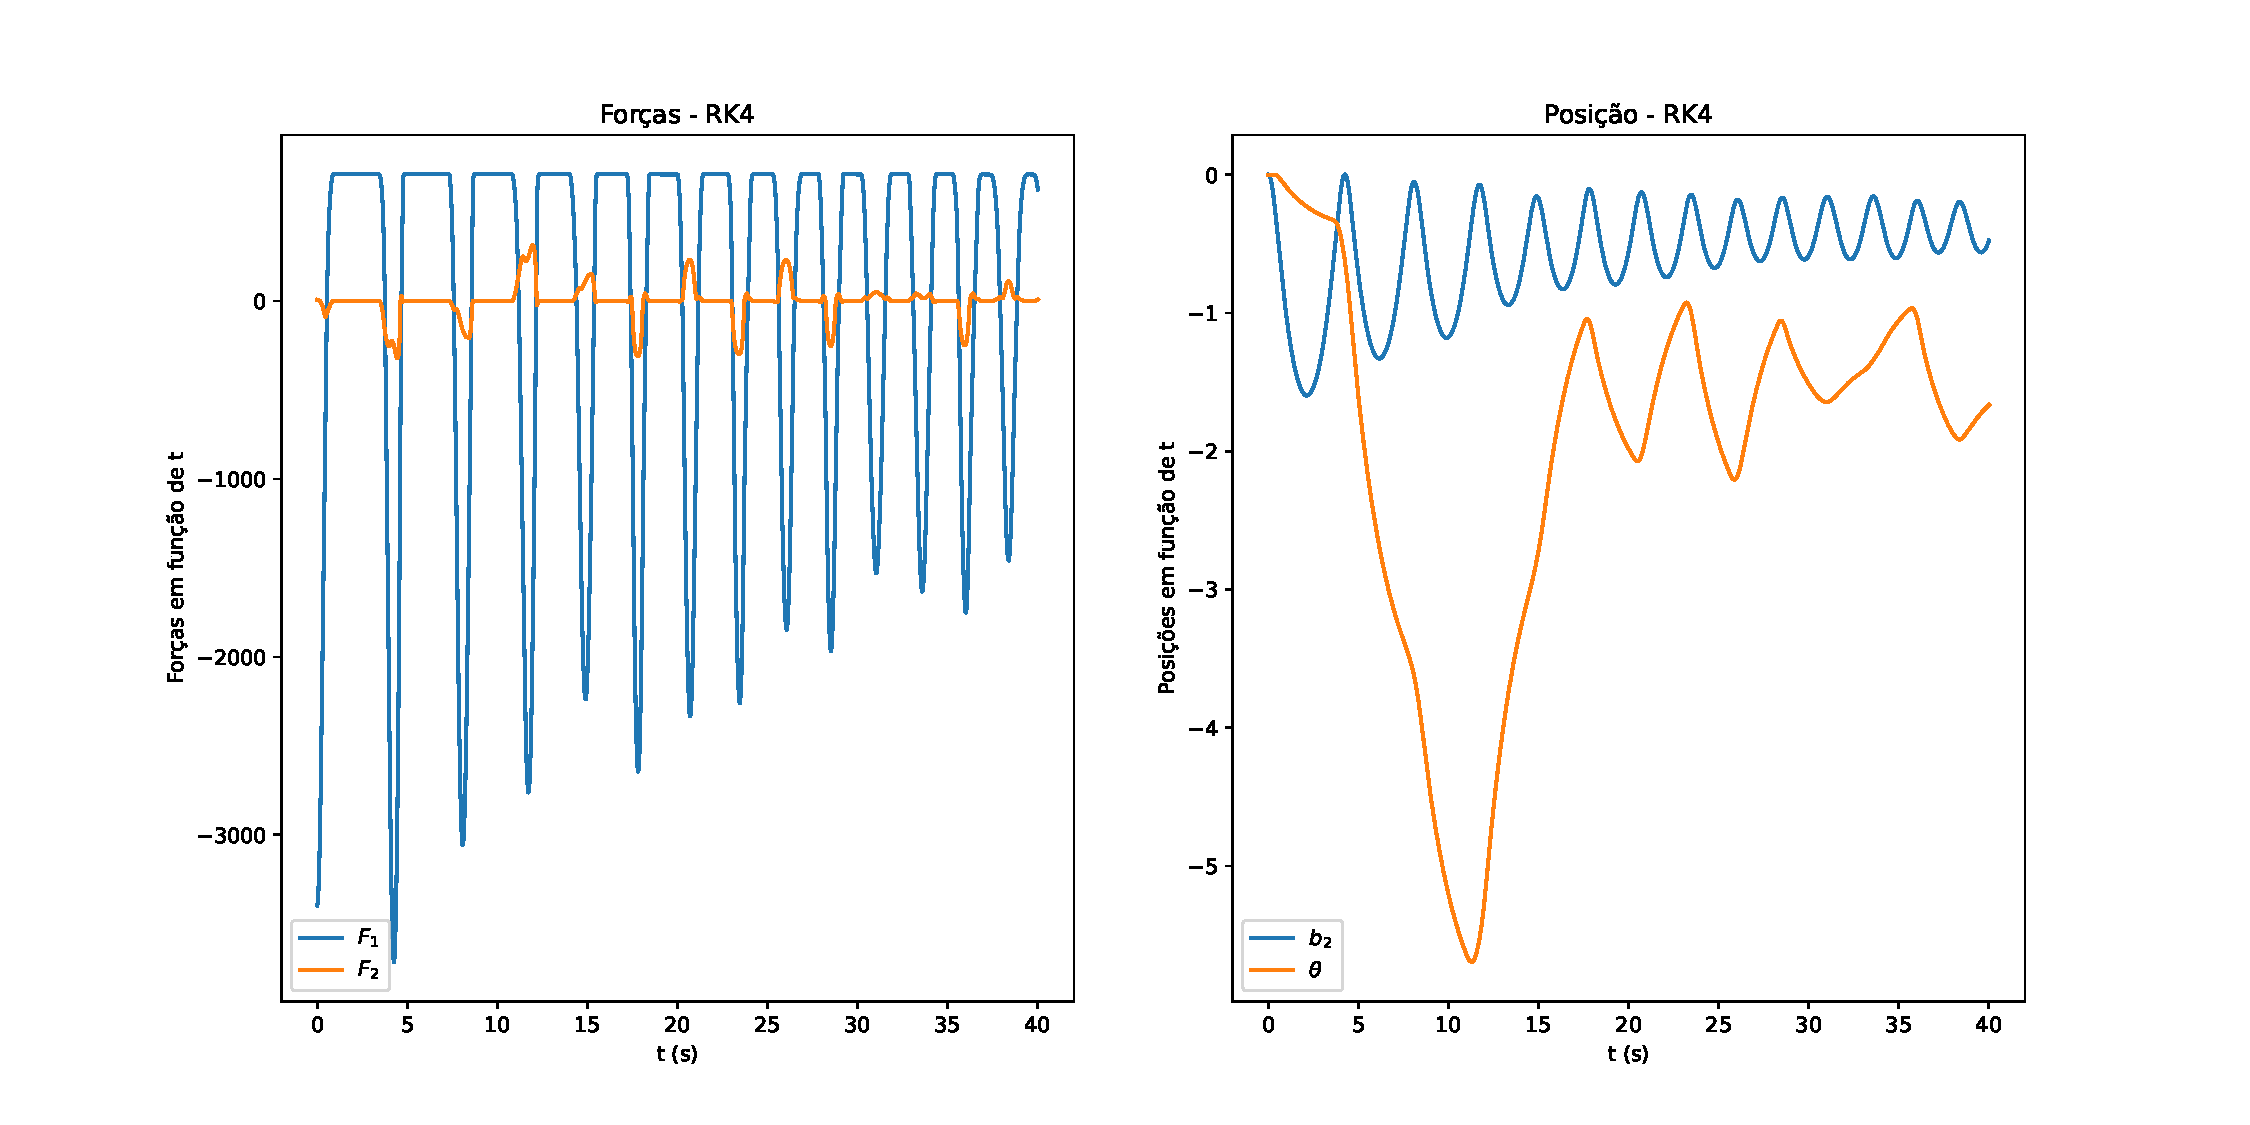
\includegraphics[width=\textwidth]{iceberg/PVI_h=0.03_g1=1.0_g2=0.5.pdf}
            \caption{$\gamma_2 = 0.5$}
        \end{subfigure}
        \quad
        \begin{subfigure}[b]{0.9\textwidth}
            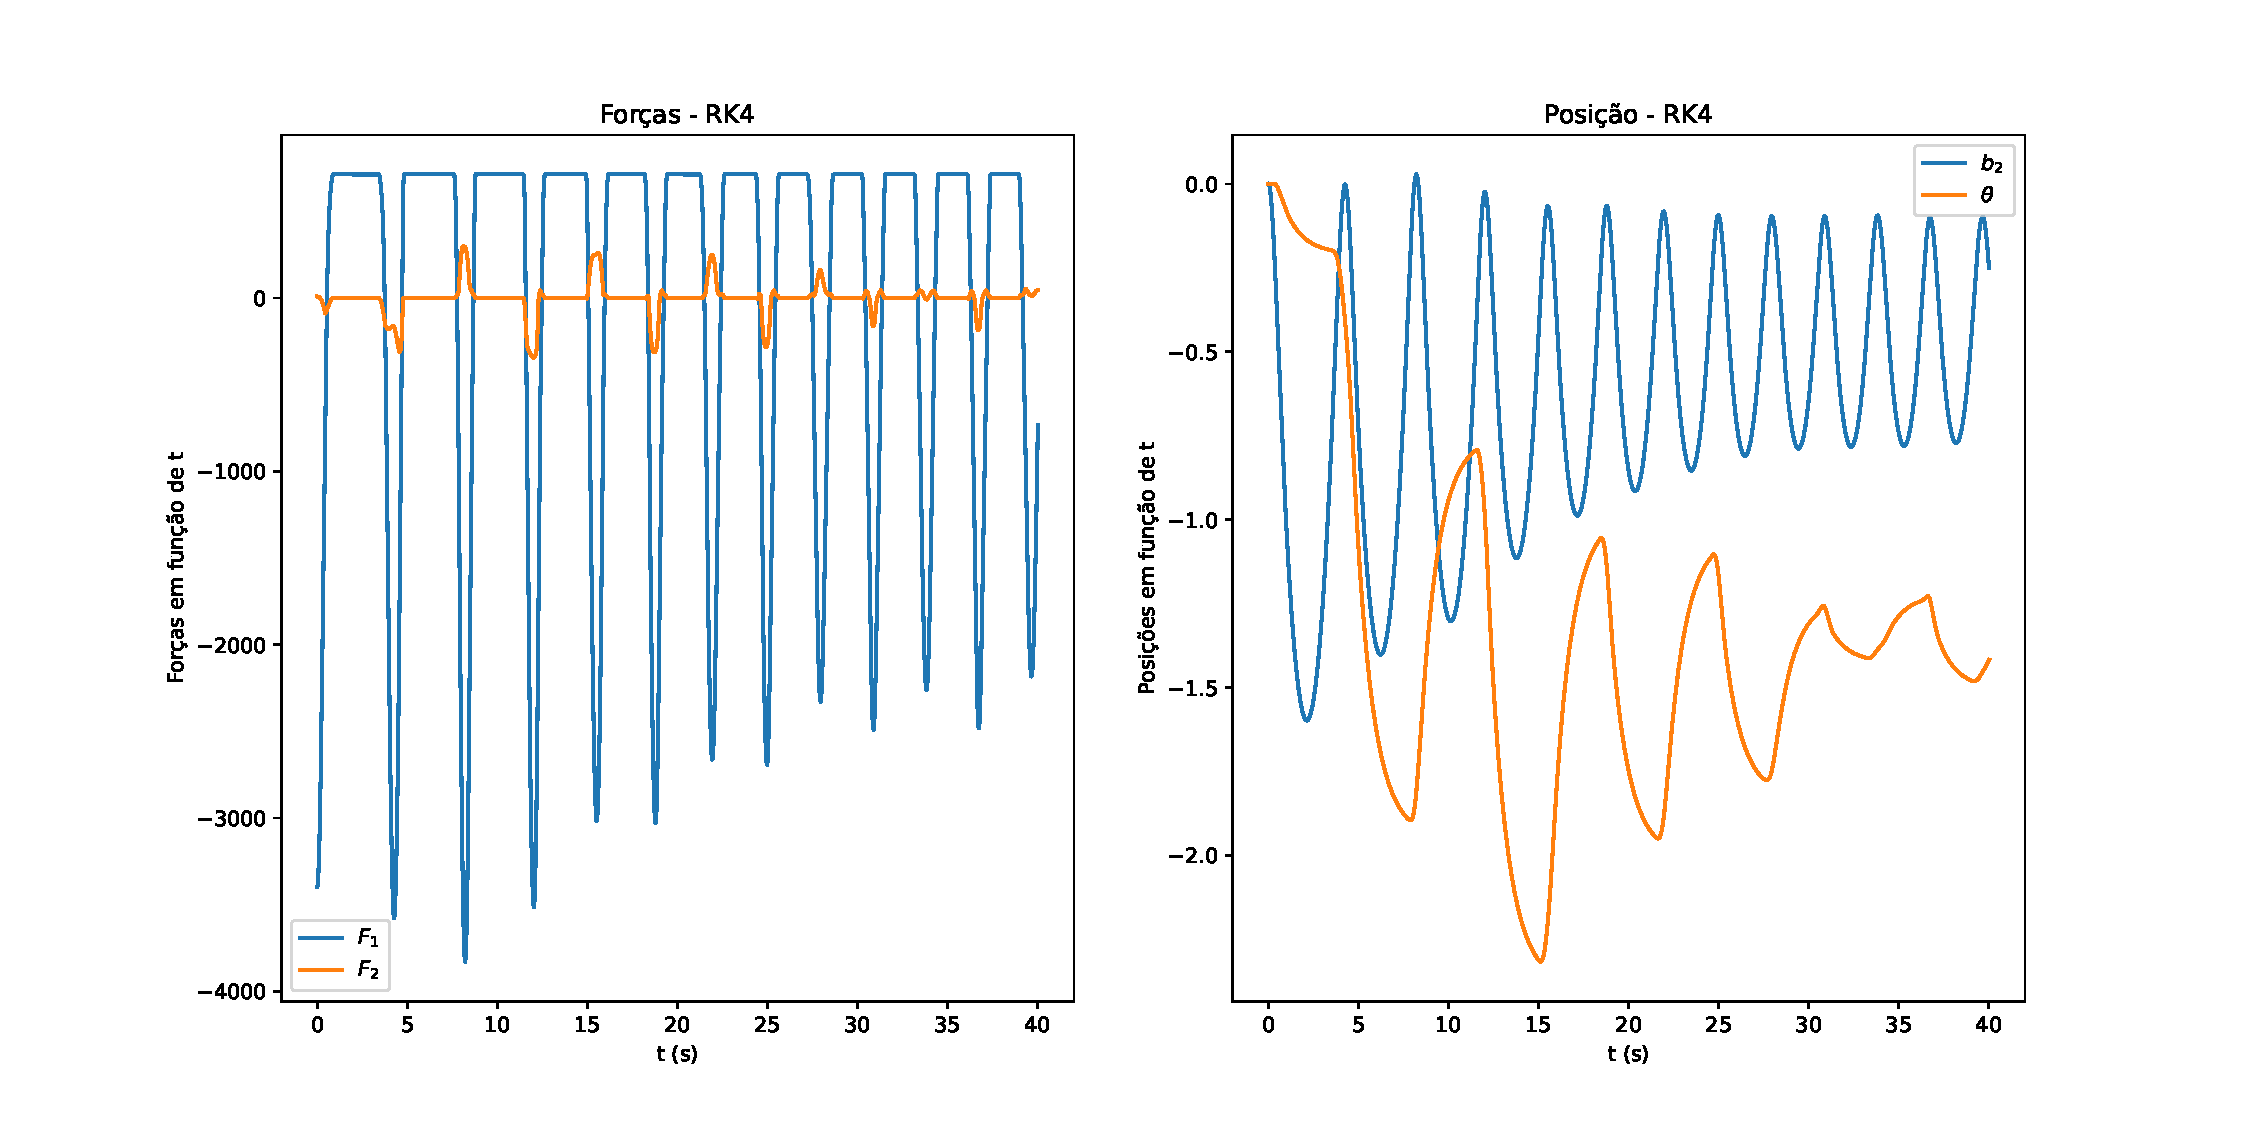
\includegraphics[width=\textwidth]{iceberg/PVI_h=0.03_g1=1.0_g2=1.0.pdf}
            \caption{$\gamma_2 = 1.0$}
        \end{subfigure}
        \quad
        \begin{subfigure}[b]{0.9\textwidth}
            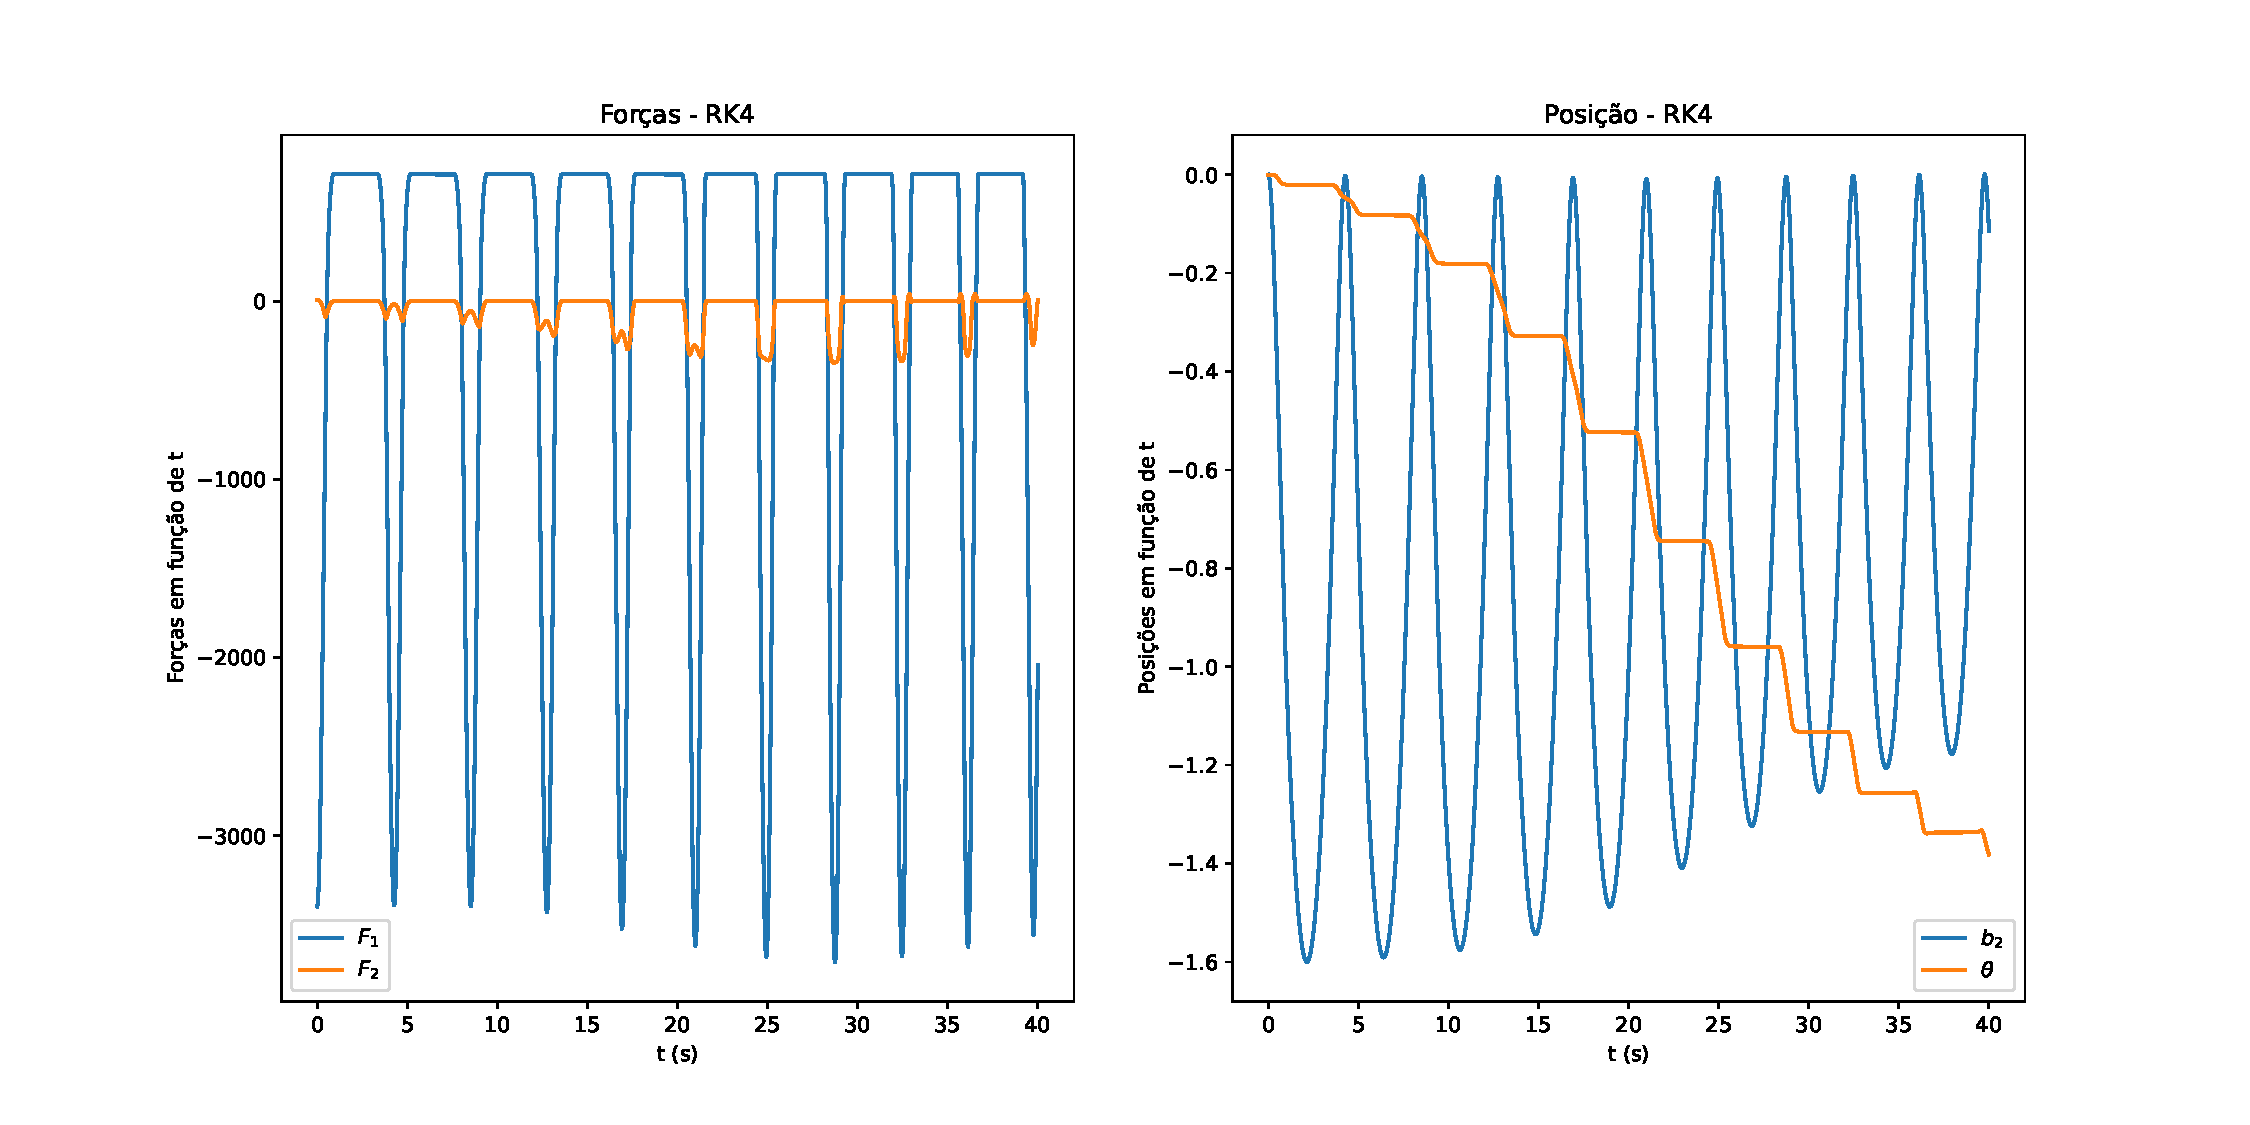
\includegraphics[width=\textwidth]{iceberg/PVI_h=0.03_g1=1.0_g2=10.0.pdf}
            \caption{$\gamma_2 = 10.0$}
        \end{subfigure}
        \caption{PVI com $\gamma_1 = 1.0$ (iceberg)}
        \label{fig:ice_PVI1}
    \end{figure}

    \begin{figure}
        \centering
        \begin{subfigure}[b]{0.9\textwidth}
            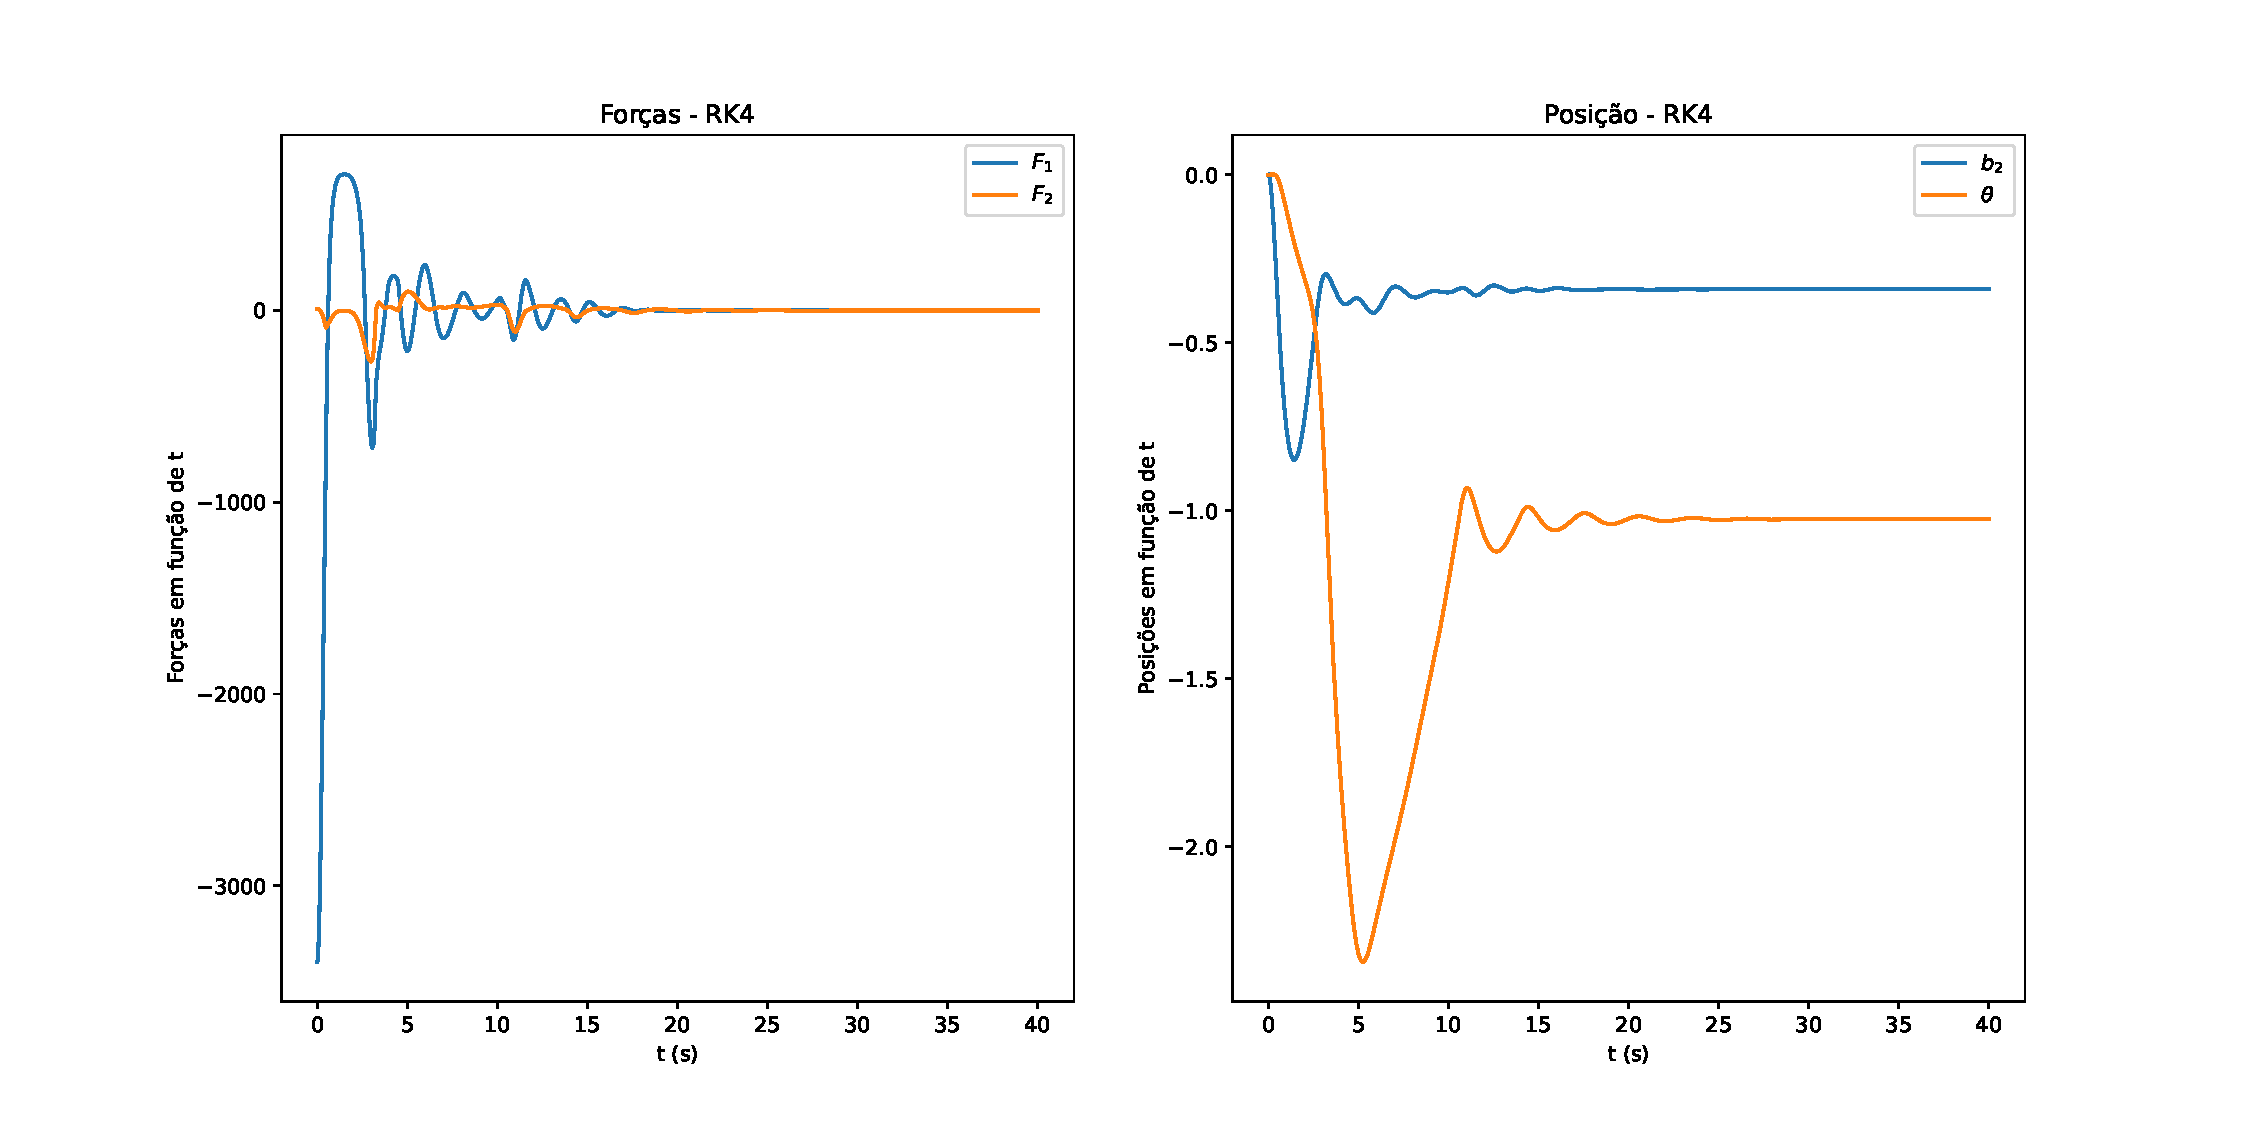
\includegraphics[width=\textwidth]{iceberg/PVI_h=0.03_g1=915.0_g2=0.5.pdf}
            \caption{$\gamma_2 = 0.5$}
        \end{subfigure}
        \quad
        \begin{subfigure}[b]{0.9\textwidth}
            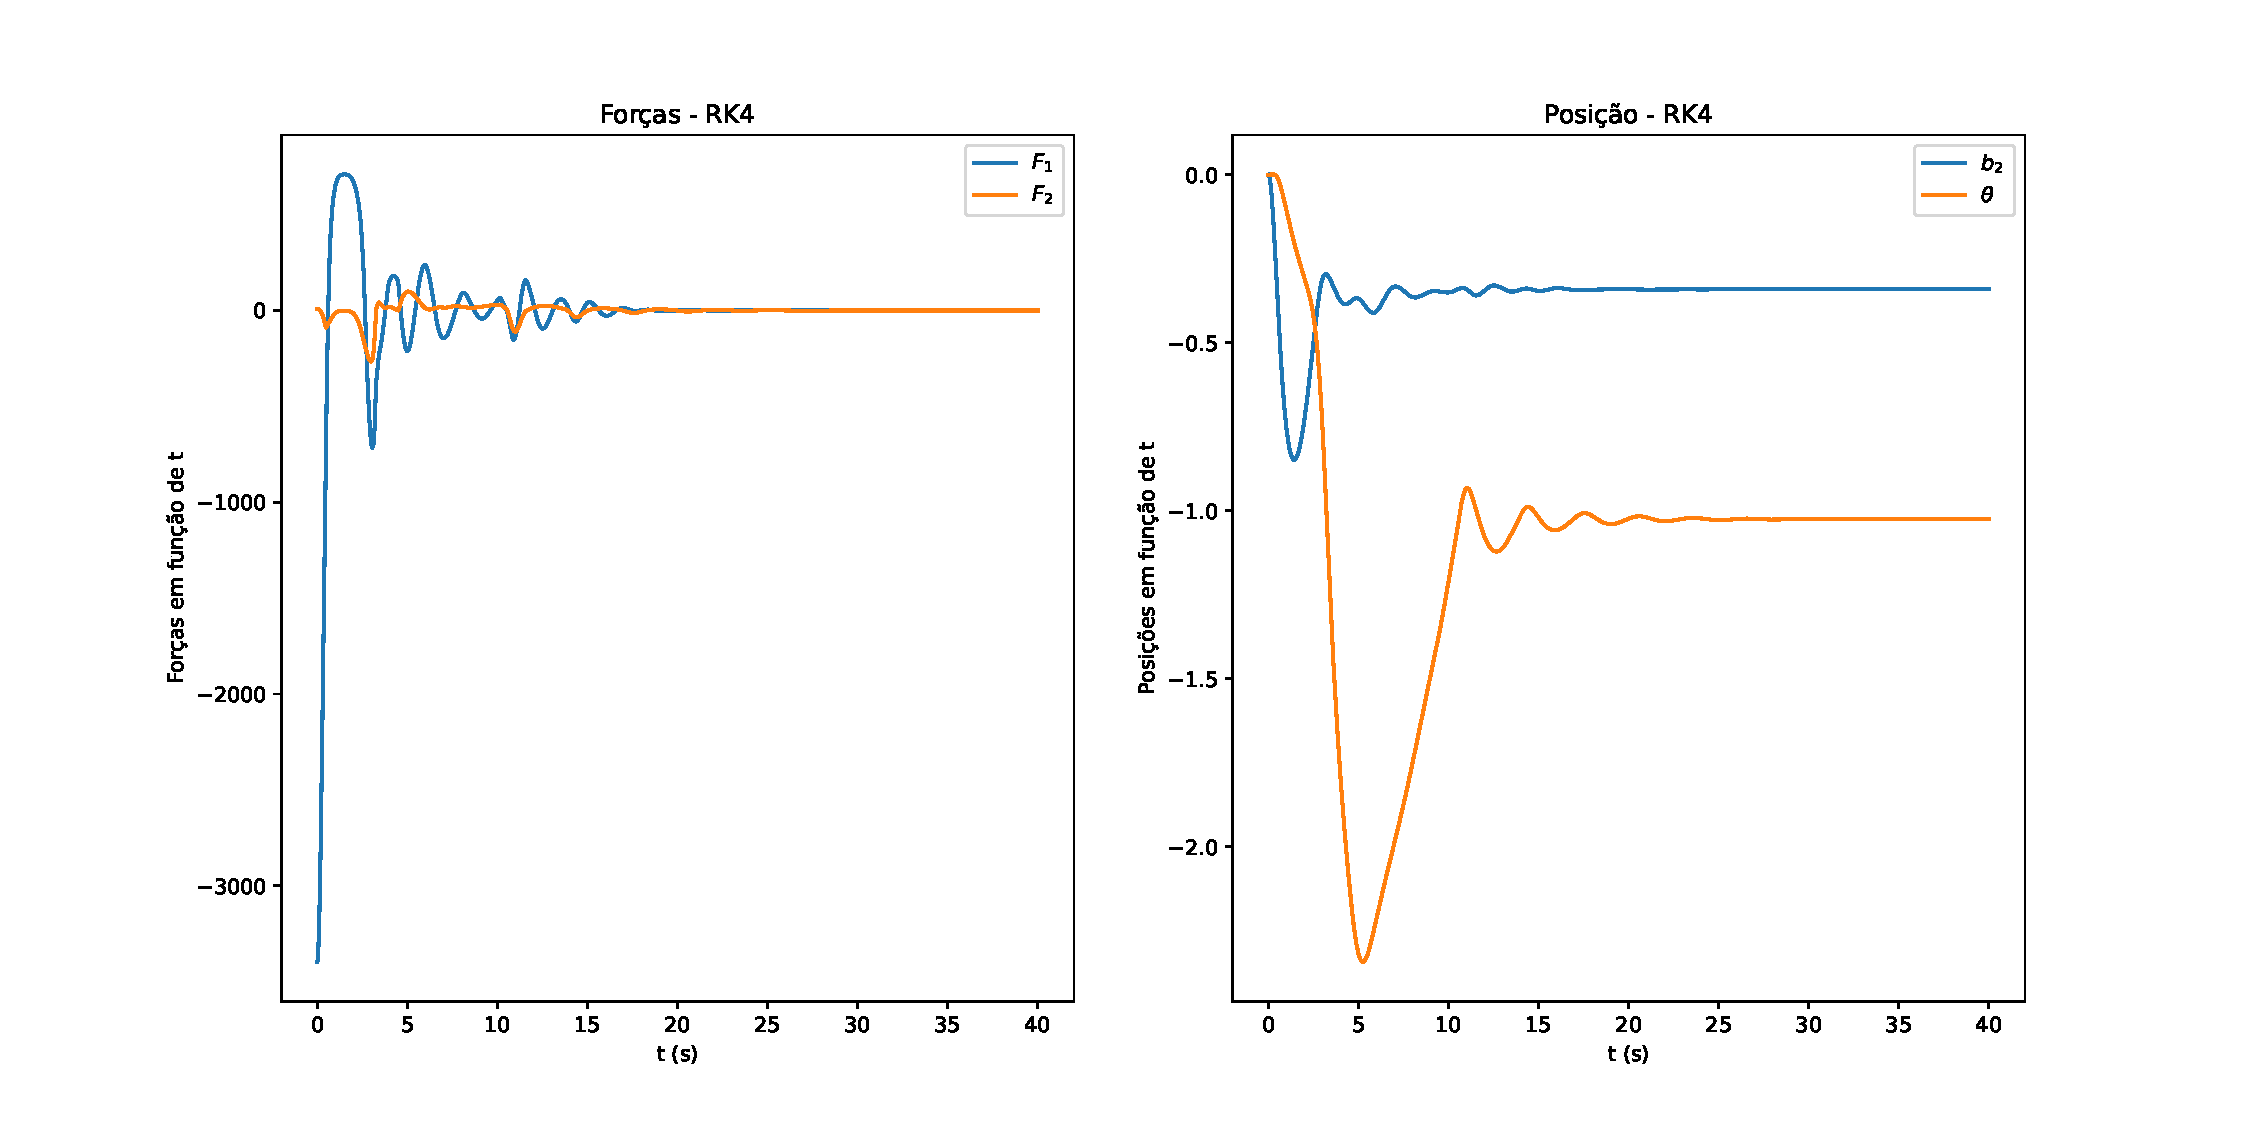
\includegraphics[width=\textwidth]{iceberg/PVI_h=0.03_g1=915.0_g2=0.5.pdf}
            \caption{$\gamma_2 = 1.0$}
        \end{subfigure}
        \quad
        \begin{subfigure}[b]{0.9\textwidth}
            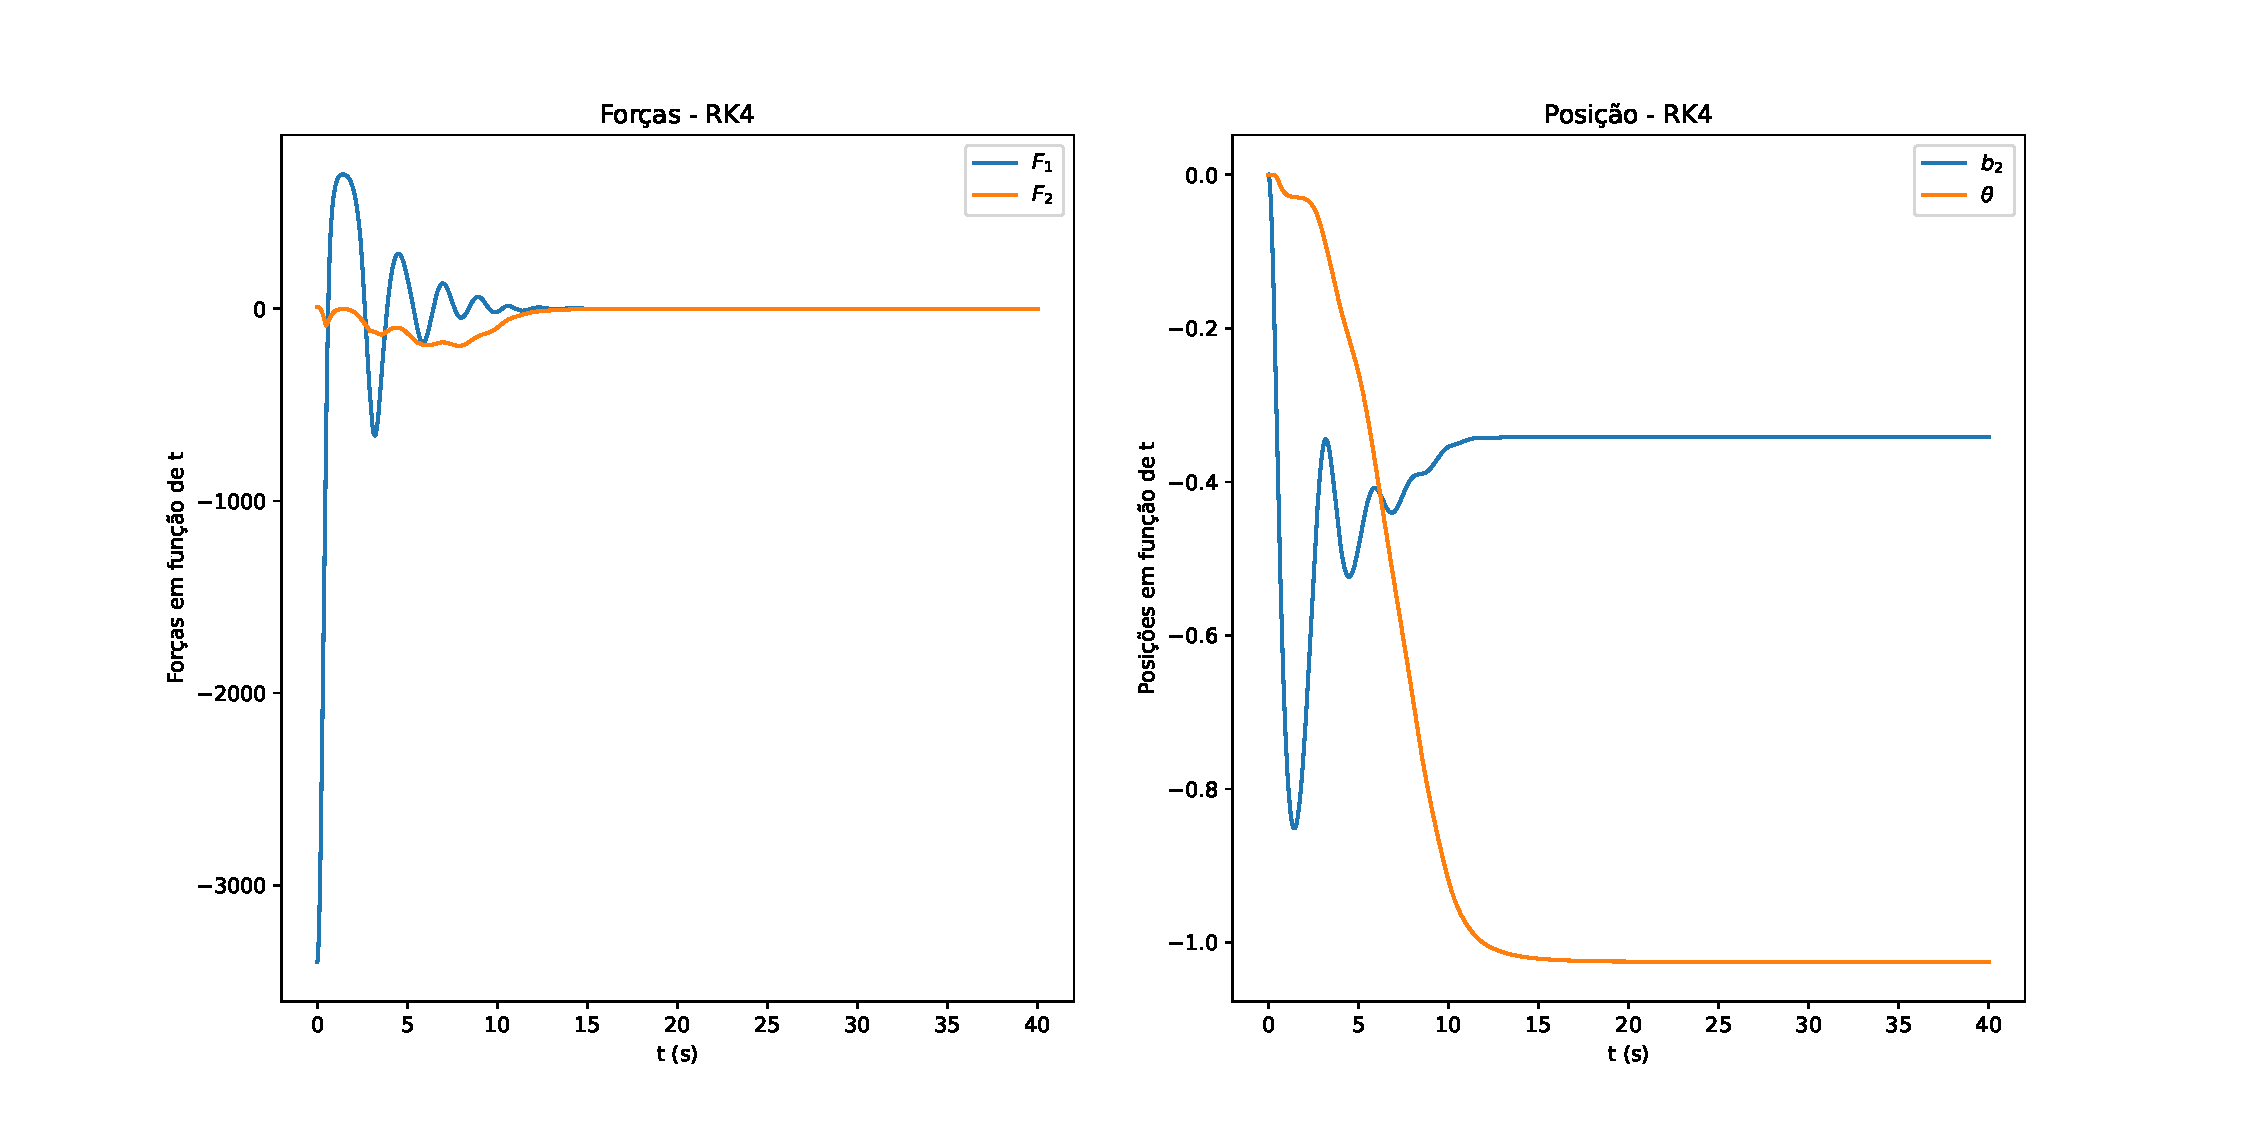
\includegraphics[width=\textwidth]{iceberg/PVI_h=0.03_g1=915.0_g2=10.0.pdf}
            \caption{$\gamma_2 = 10.0$}
        \end{subfigure}
        \caption{PVI com $\gamma_1 = 915.0$ (iceberg)}
        \label{fig:ice_PVI2}
    \end{figure}

    \begin{figure}
        \centering
        \begin{subfigure}[b]{0.9\textwidth}
            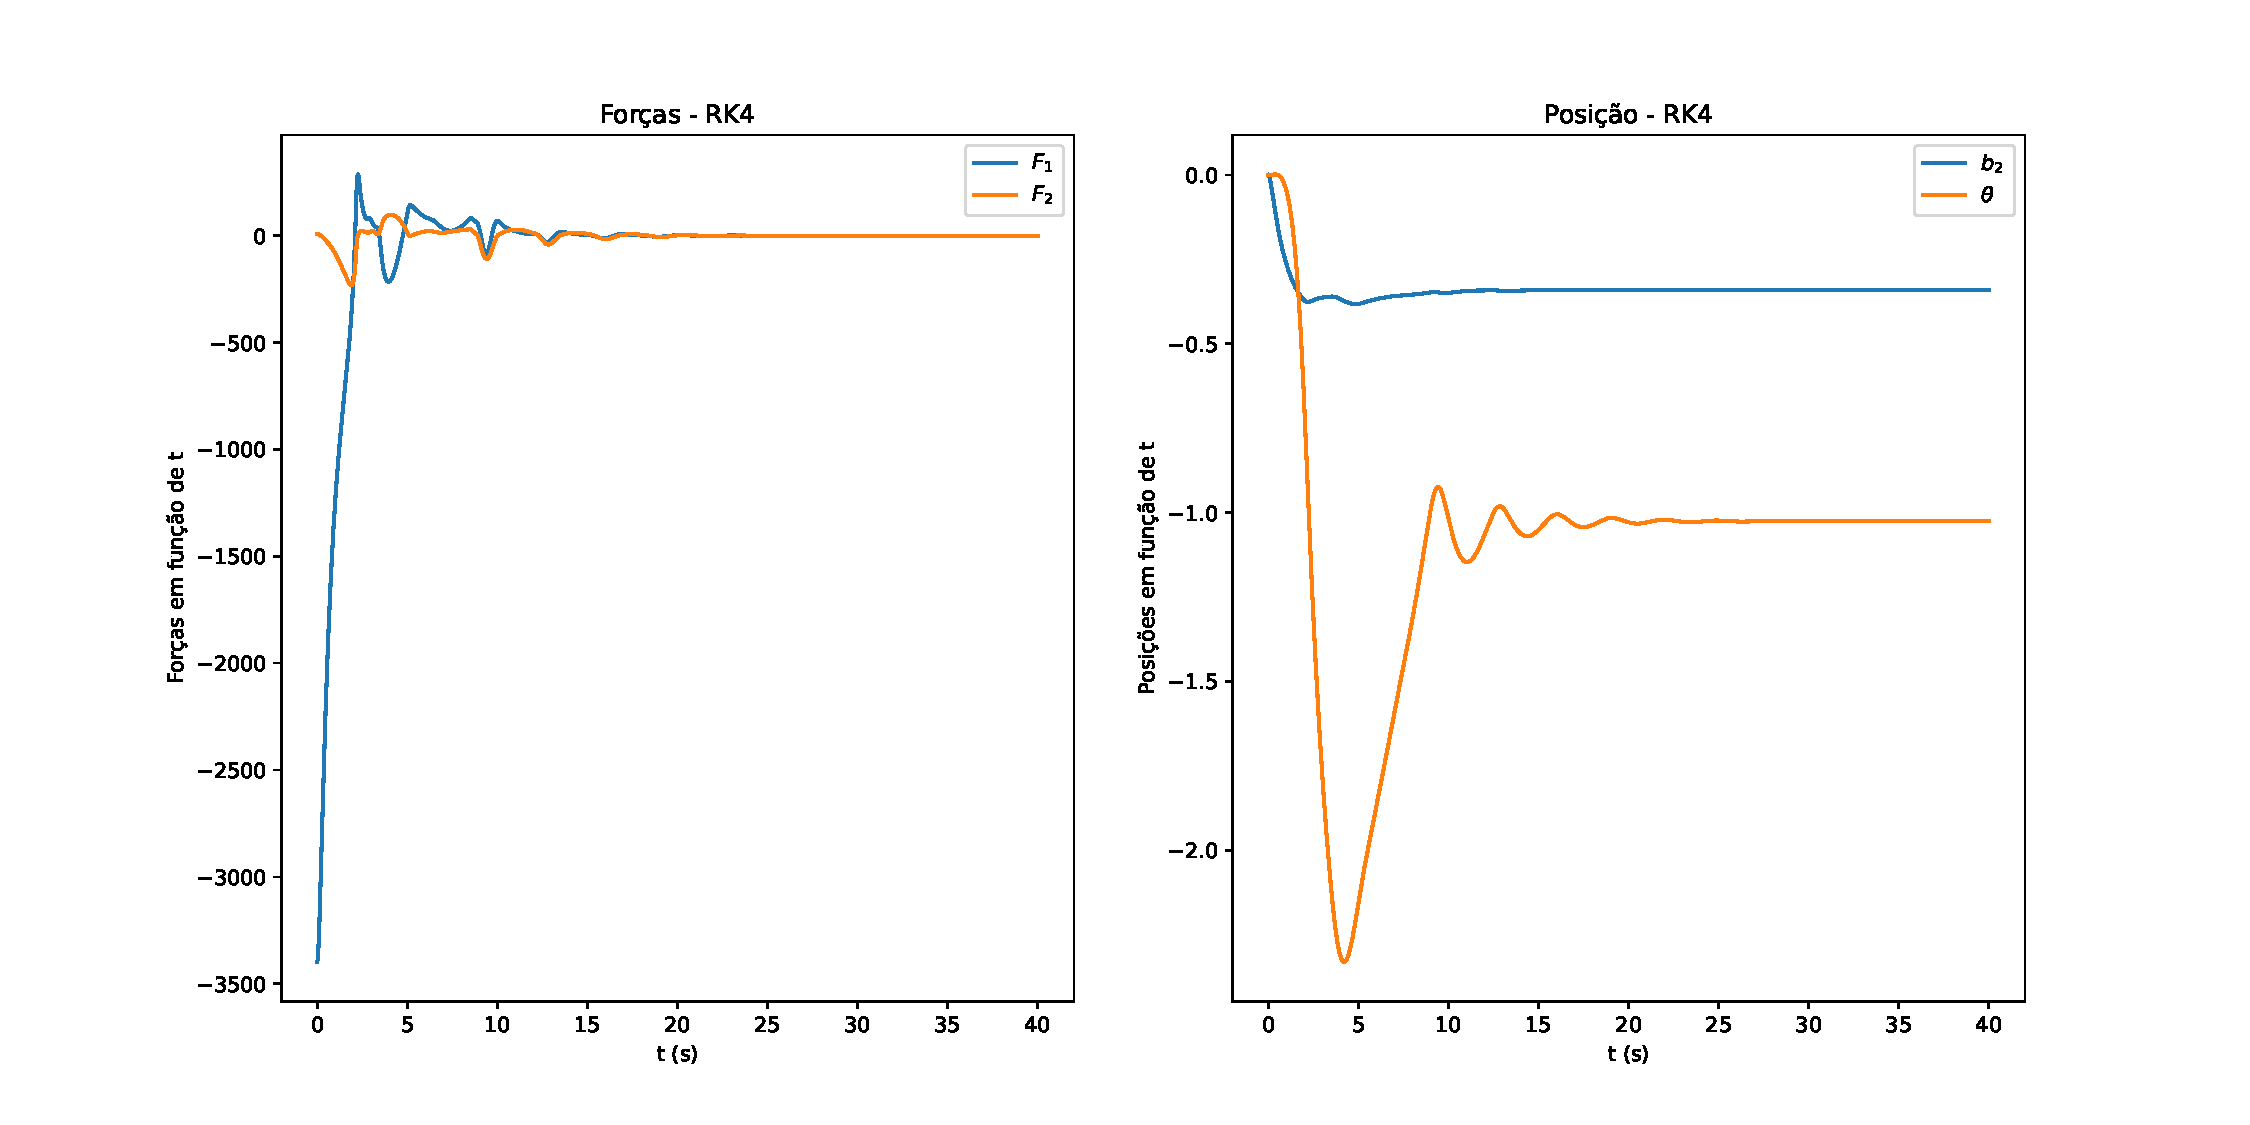
\includegraphics[width=\textwidth]{iceberg/PVI_h=0.03_g1=9000.0_g2=0.5.pdf}
            \caption{$\gamma_2 = 0.5$}
        \end{subfigure}
        \quad
        \begin{subfigure}[b]{0.9\textwidth}
            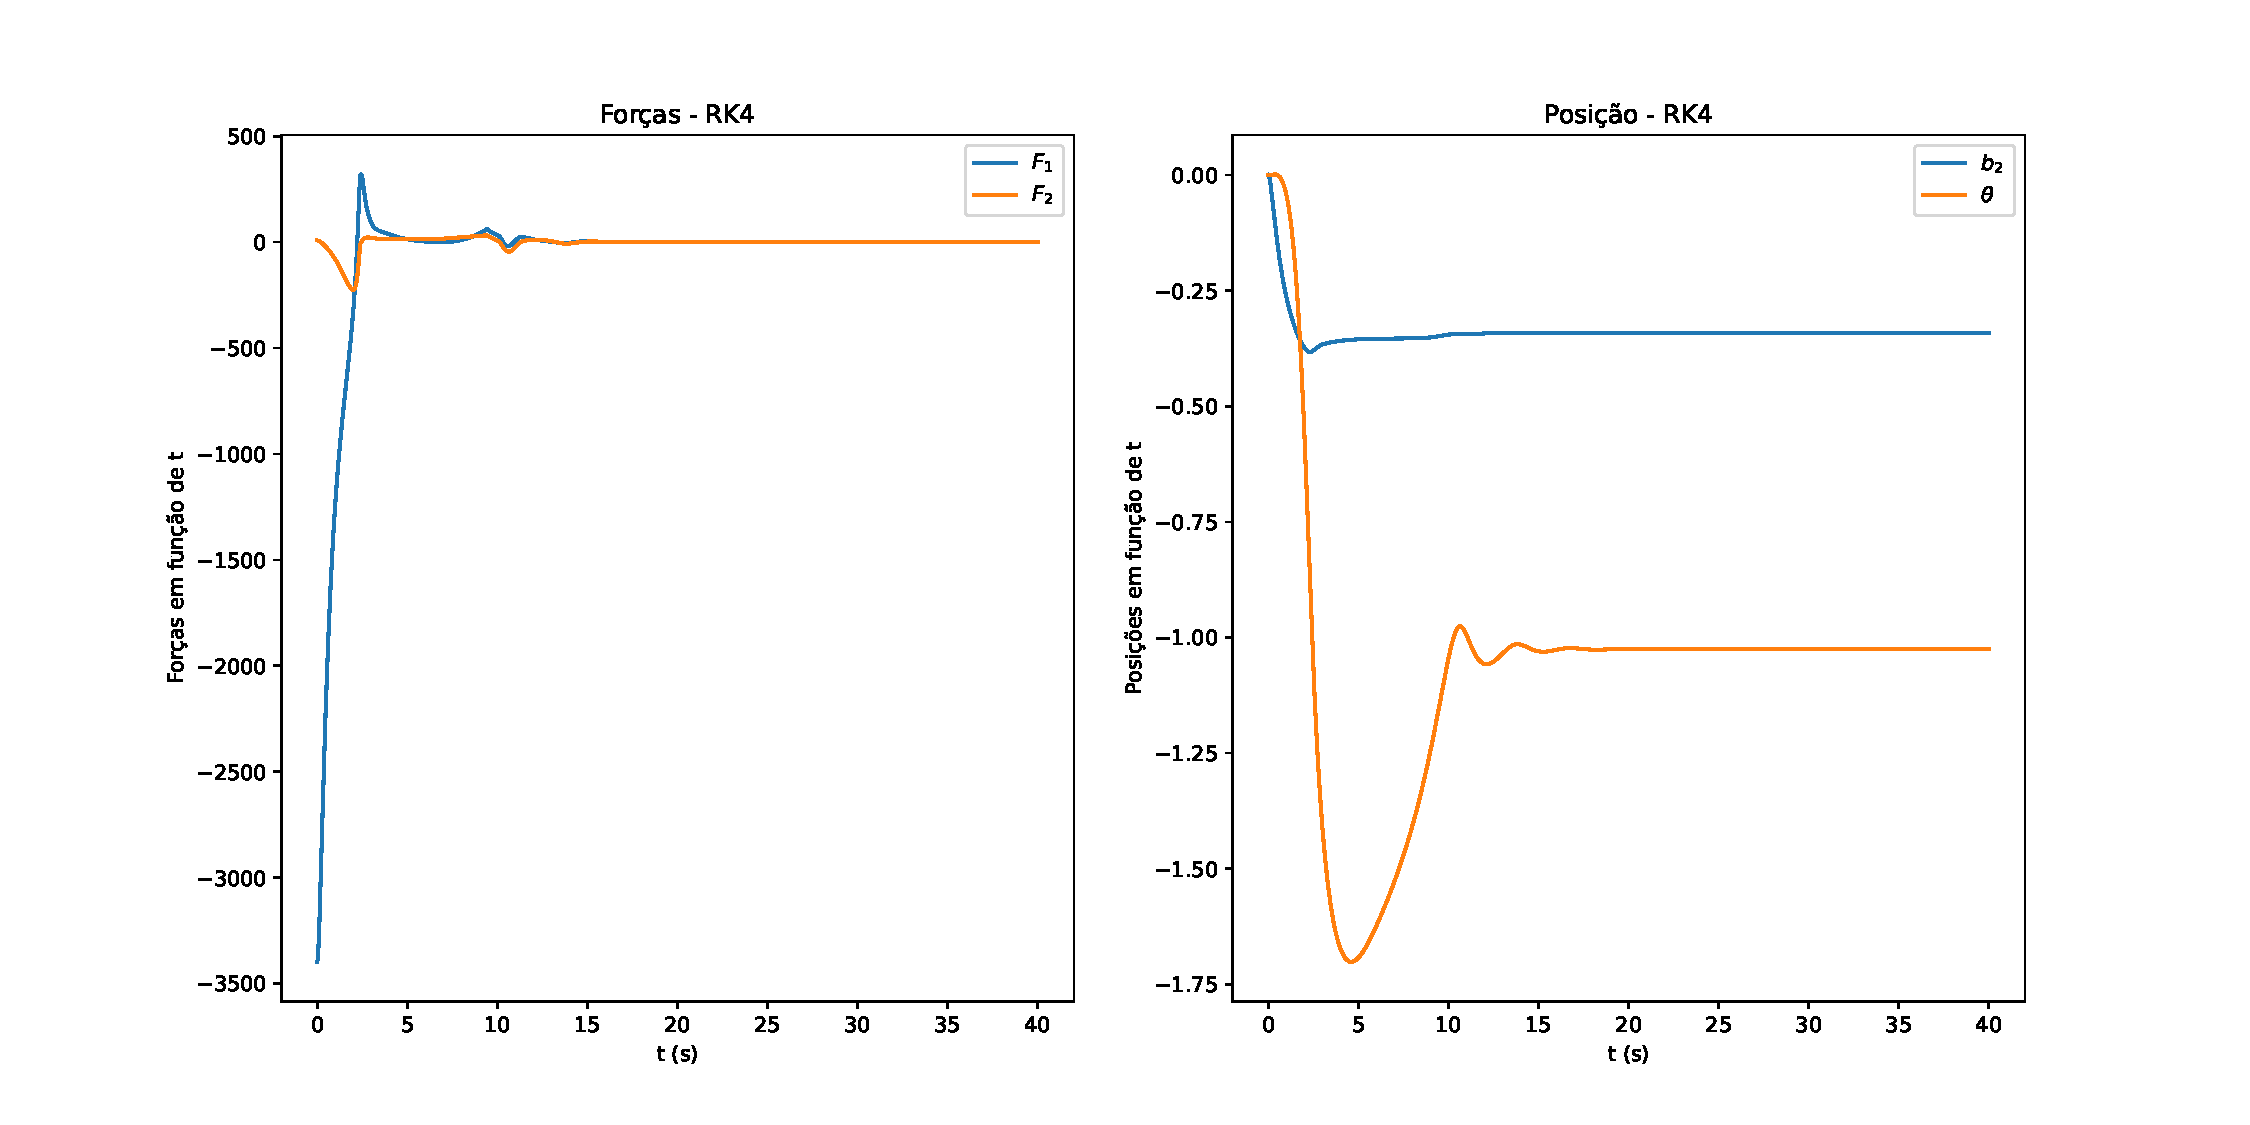
\includegraphics[width=\textwidth]{iceberg/PVI_h=0.03_g1=9000.0_g2=1.0.pdf}
            \caption{$\gamma_2 = 1.0$}
        \end{subfigure}
        \quad
        \begin{subfigure}[b]{0.9\textwidth}
            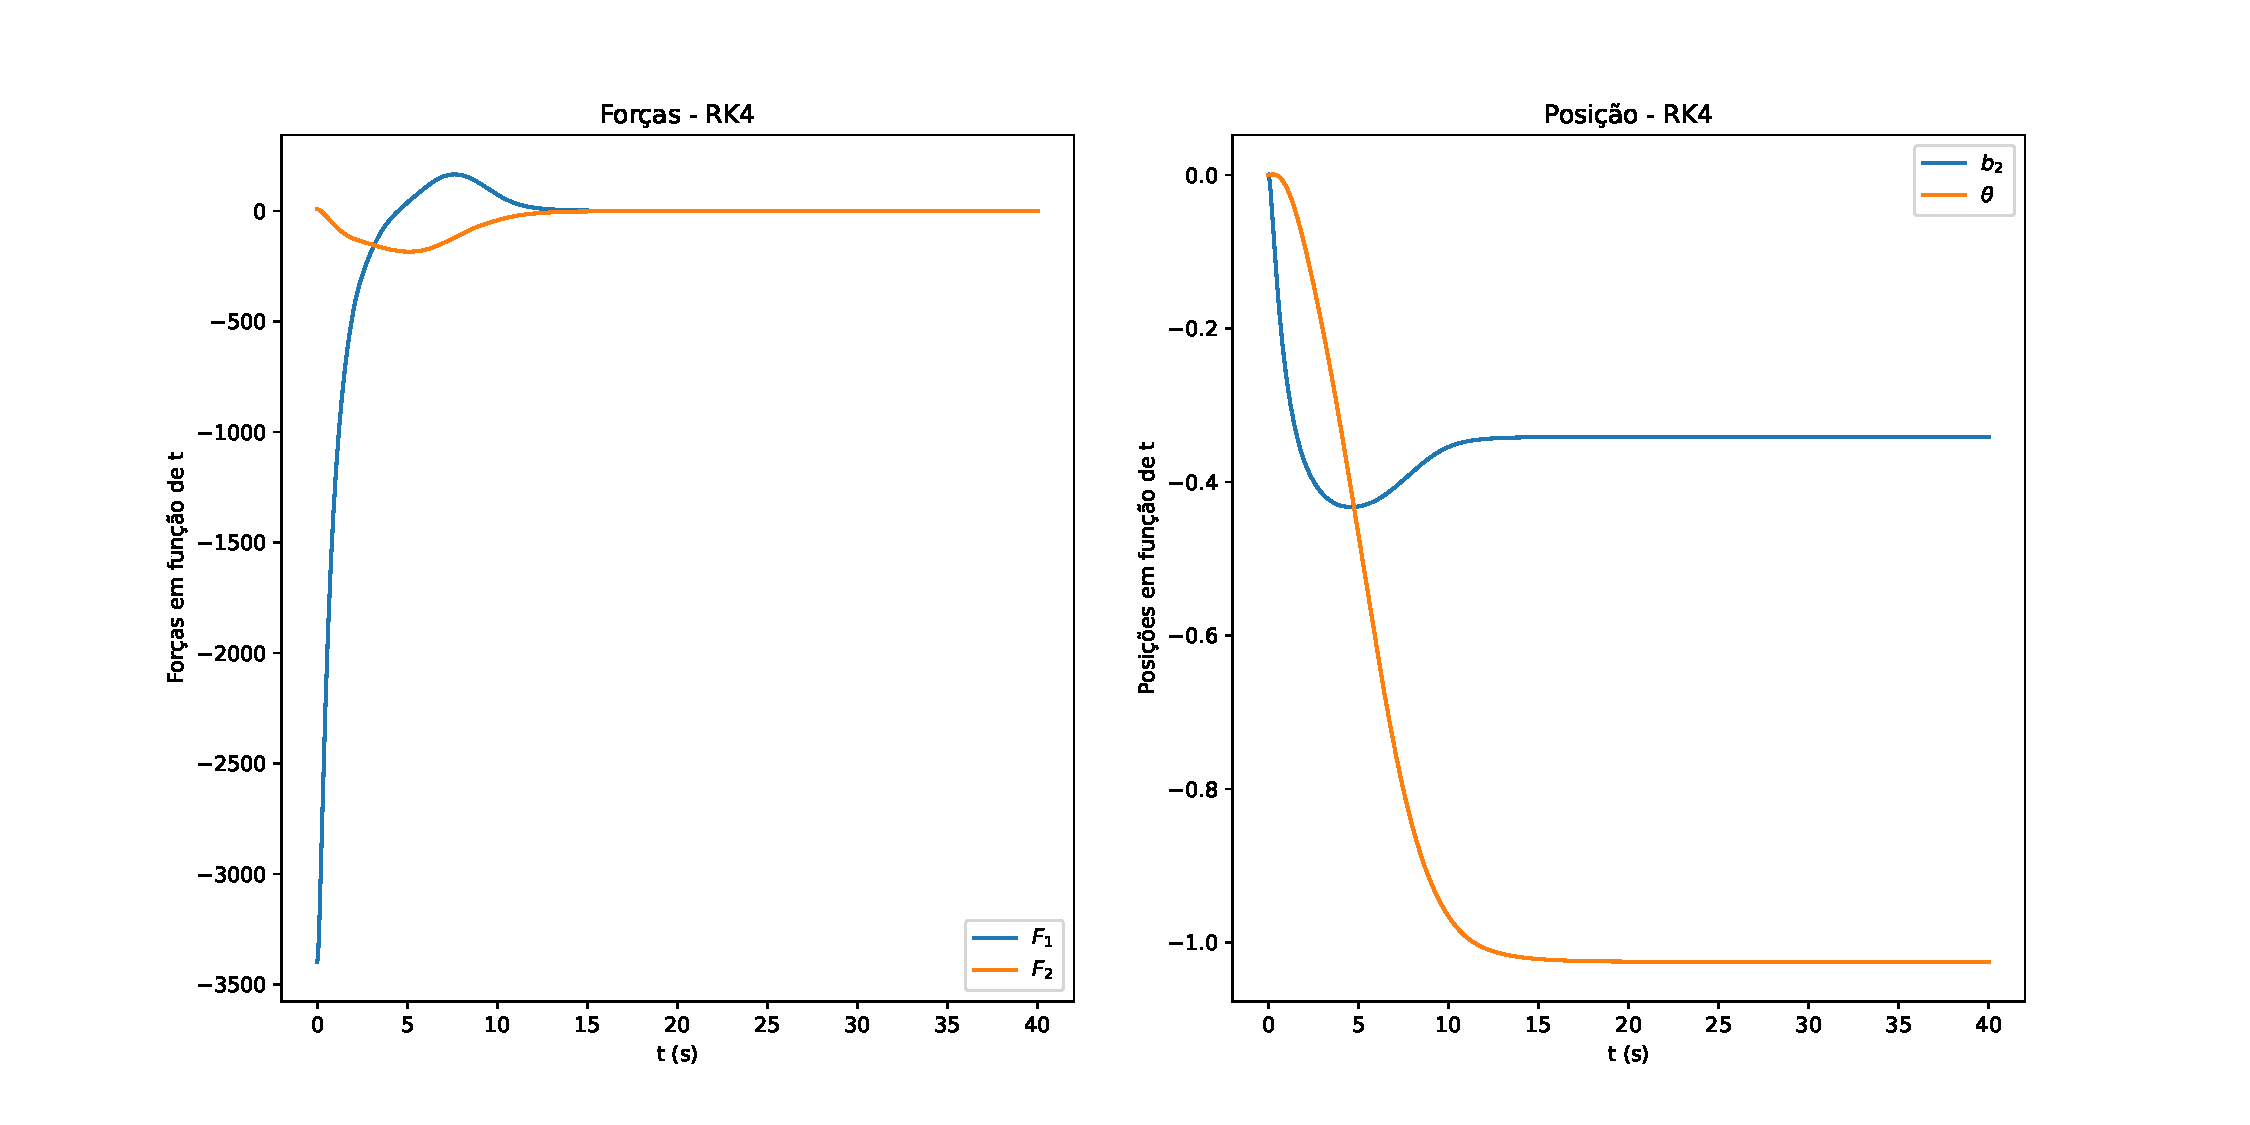
\includegraphics[width=\textwidth]{iceberg/PVI_h=0.03_g1=9000.0_g2=10.0.pdf}
            \caption{$\gamma_2 = 10.0$}
        \end{subfigure}
        \caption{PVI com $\gamma_1 = 9000.0$ (iceberg)}
        \label{fig:ice_PVI3}
    \end{figure}

    Como a densidade do iceberg é $917kg/m^3$ e iniciamos ele com o centro de massa na origem, sua força peso começa muito maior que o empuxo, fazendo com que ele afunde. Nos casos em que os coeficientes de amortecimentos são mais baixos, isso pode gerar um movimento imprevisível para $\theta$.

    É evidenciado um forte acoplamento no PVI entre as variáveis $\theta$ e $b_2$. Nas situações em que os coeficientes de amortecimento tem grandeza desproporcionais, a variável com coeficiente mais baixo acaba por oscilar como reação à oscilação da outra variável.

    Por fim, para os casos que chegaram no equilíbrio dentro do tempo da simulação, o ponto de estado estacionário foi o ponto 4. Note que o valor de $\theta$ final para o PVI e do ponto encontrado pelo método de Newton diferem por $2\pi$, o que significa que a posição do corpo é essencialmente a mesma.
    \FloatBarrier

    Foi analisada também a convergência do PVI em função do passo de tempo. Para isso, foi utilizada a norma $L^2$ discreta com relação a uma malha fina. Foram escolhidos $c_1 = 1$ e $c_2 = 1$.

    \begin{figure}[H]
        \centering
        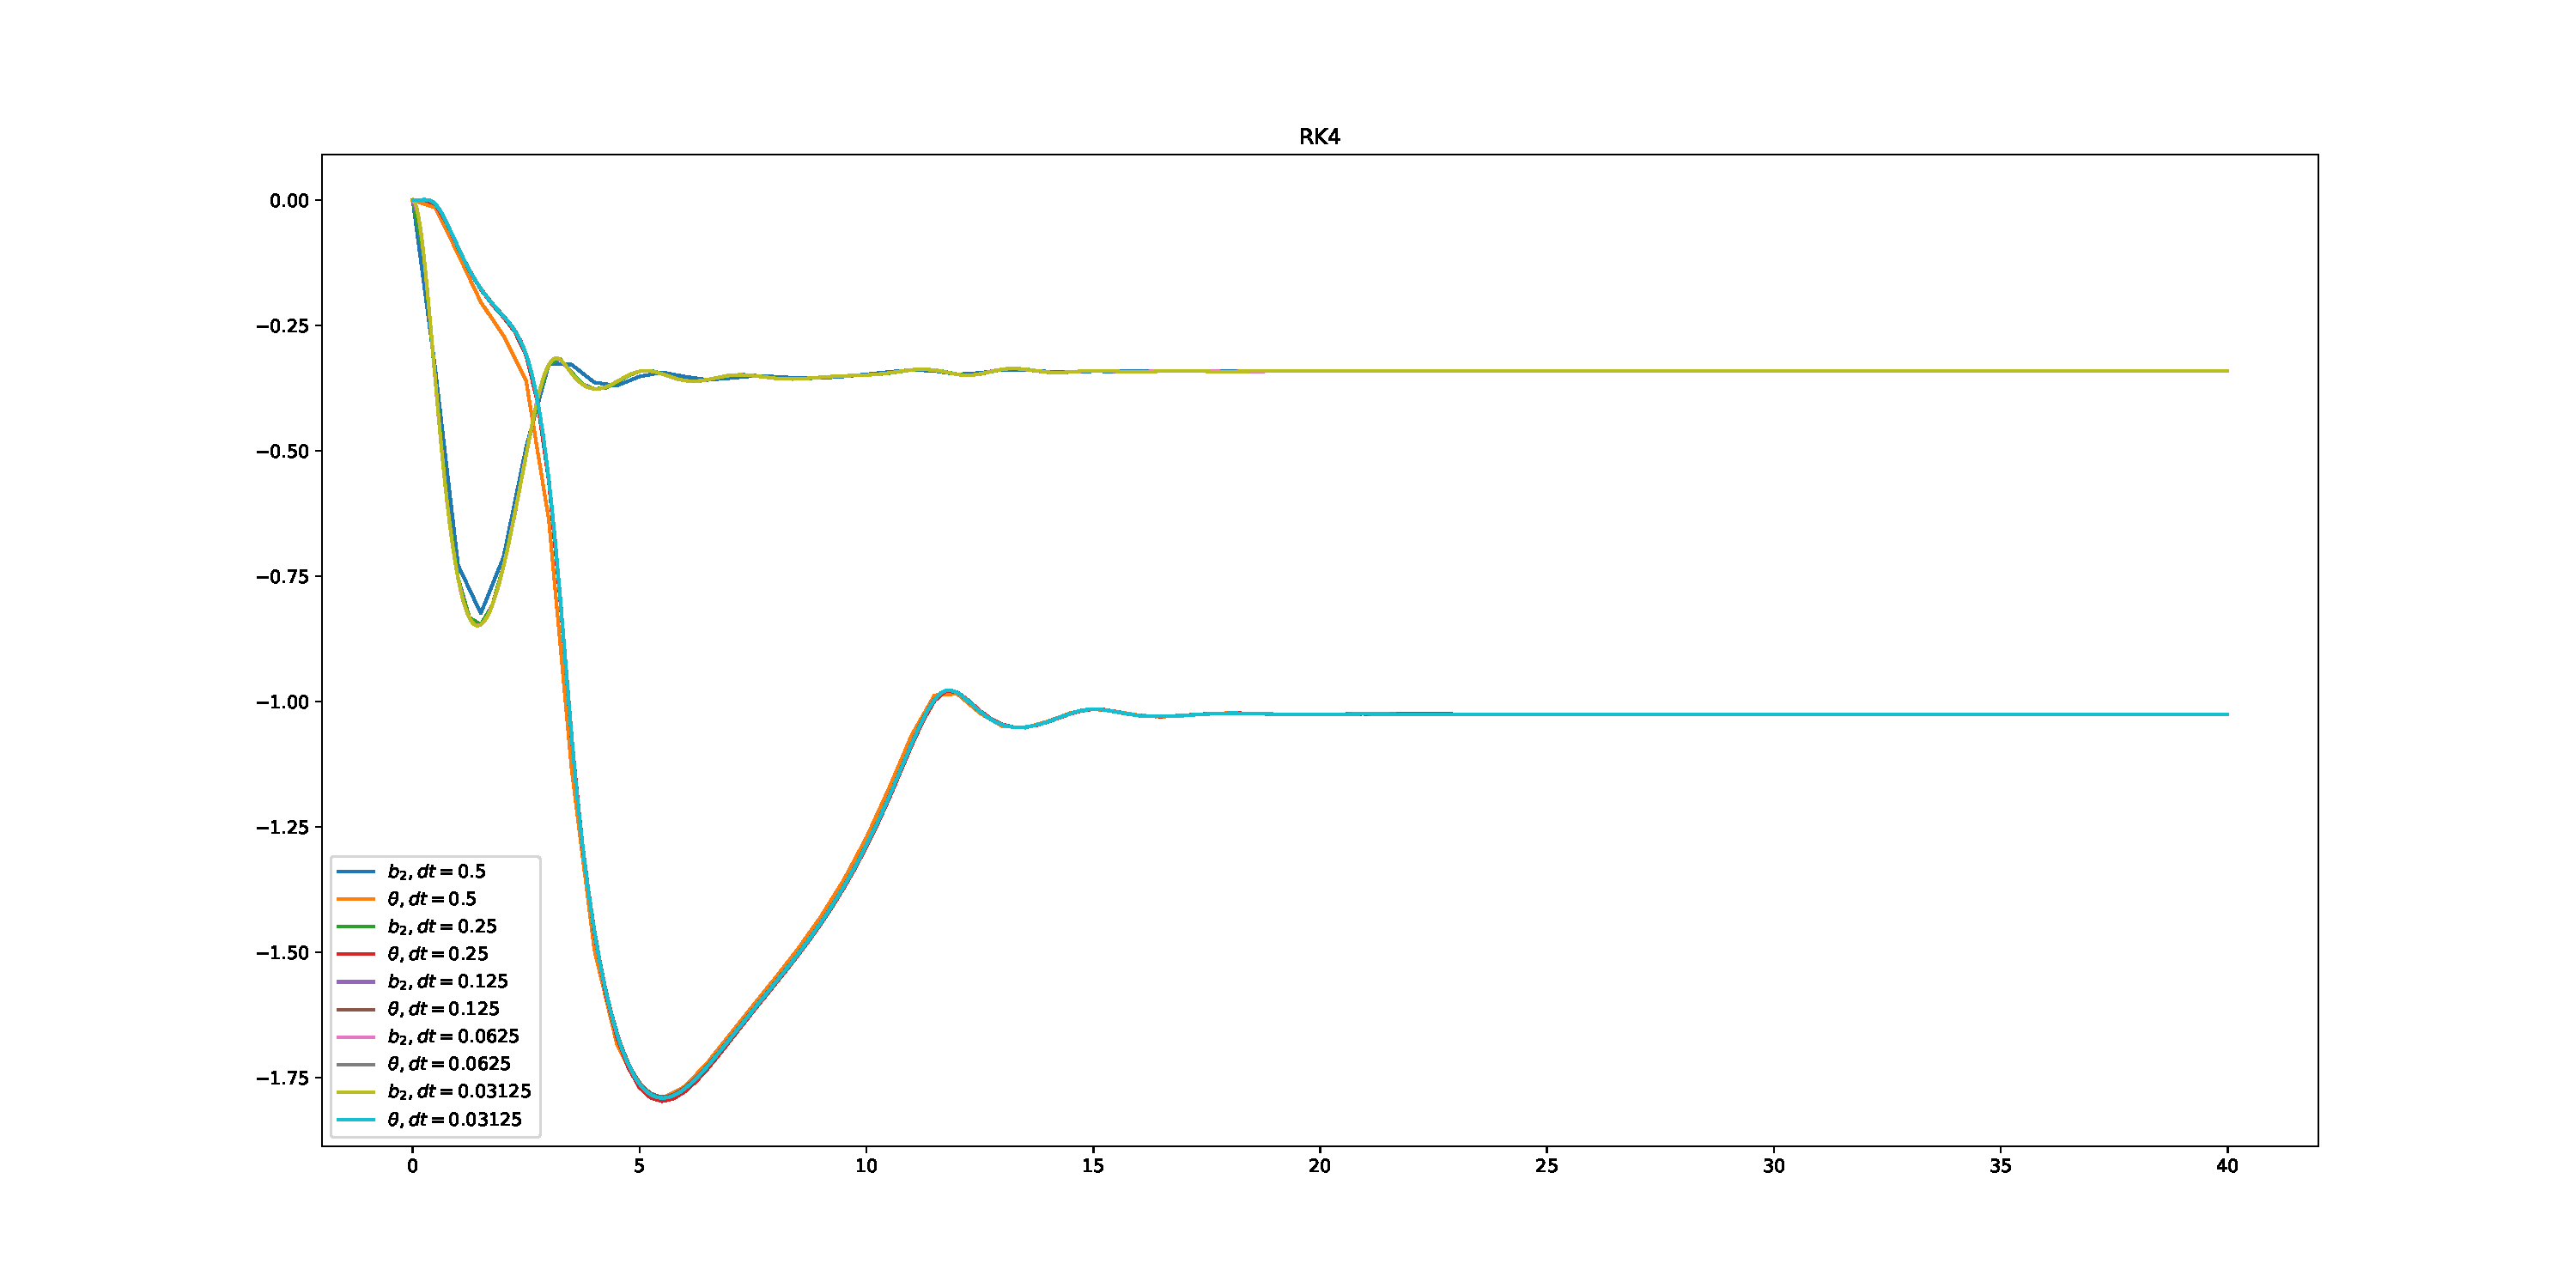
\includegraphics[width=\textwidth]{iceberg/PVI_conv.pdf}
        \caption{$\theta$ e $b_2$ em função do tempo para diversos passos de tempo no caso do iceberg}
        \label{fig:ice_conv1}
    \end{figure}

    \begin{figure}[H]
        \centering
        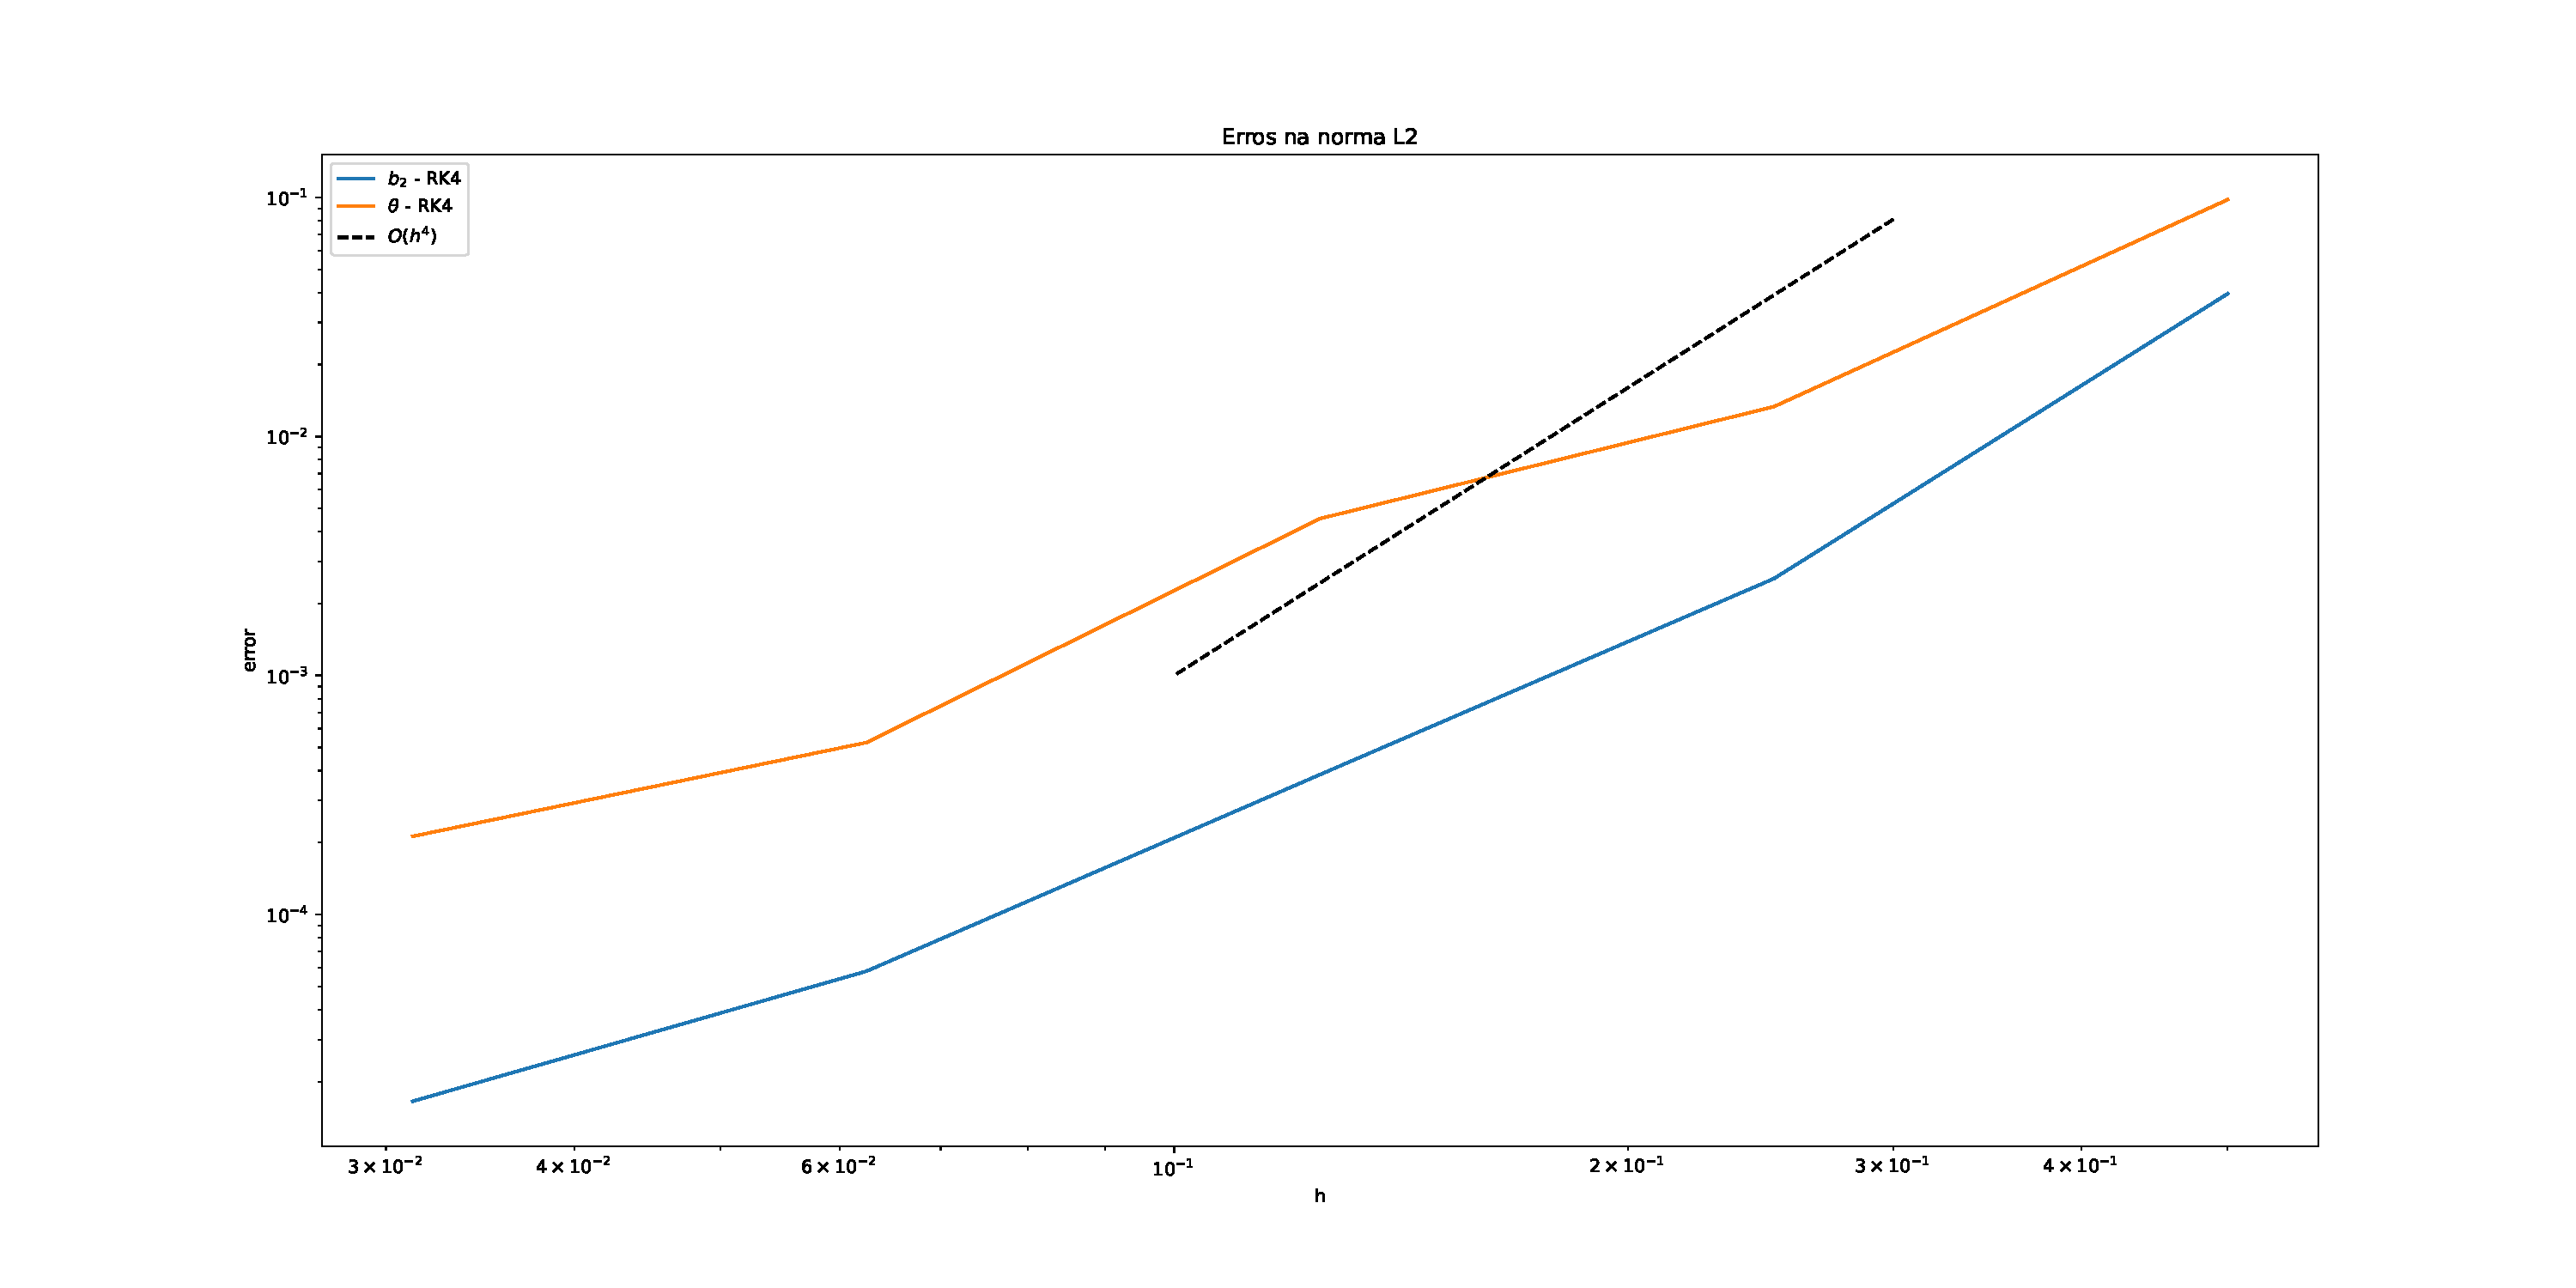
\includegraphics[width=\textwidth]{iceberg/PVI_conv2.pdf}
        \caption{Ordem de convergência do método para solução do PVI (iceberg)}
        \label{fig:ice_conv2}
    \end{figure}

    Baseado na figura \ref{fig:ice_conv1}, todas as soluções obtidas com os diferentes passos de tempo aparentam concordar na solução. De acordo com a figura \ref{fig:ice_conv2}, a ordem de convergência aparenta ser menor do que $O(h^4)$, que é a ordem esperada do método RK4.

    \FloatBarrier
    
    

    \subsection{Titanic}
    Nessa seção e na seção \ref{sec:triang}, as análises serão análogas às da seção \ref{sec:ice}, por isso, algumas etapas podem ser omitidos.

    \subsubsection{Mapeamento de forças}
    O mapa de forças para o Titanic pode ser visto na figura \ref{fig:titanic_level}.

    \begin{figure}[H]
        \centering
        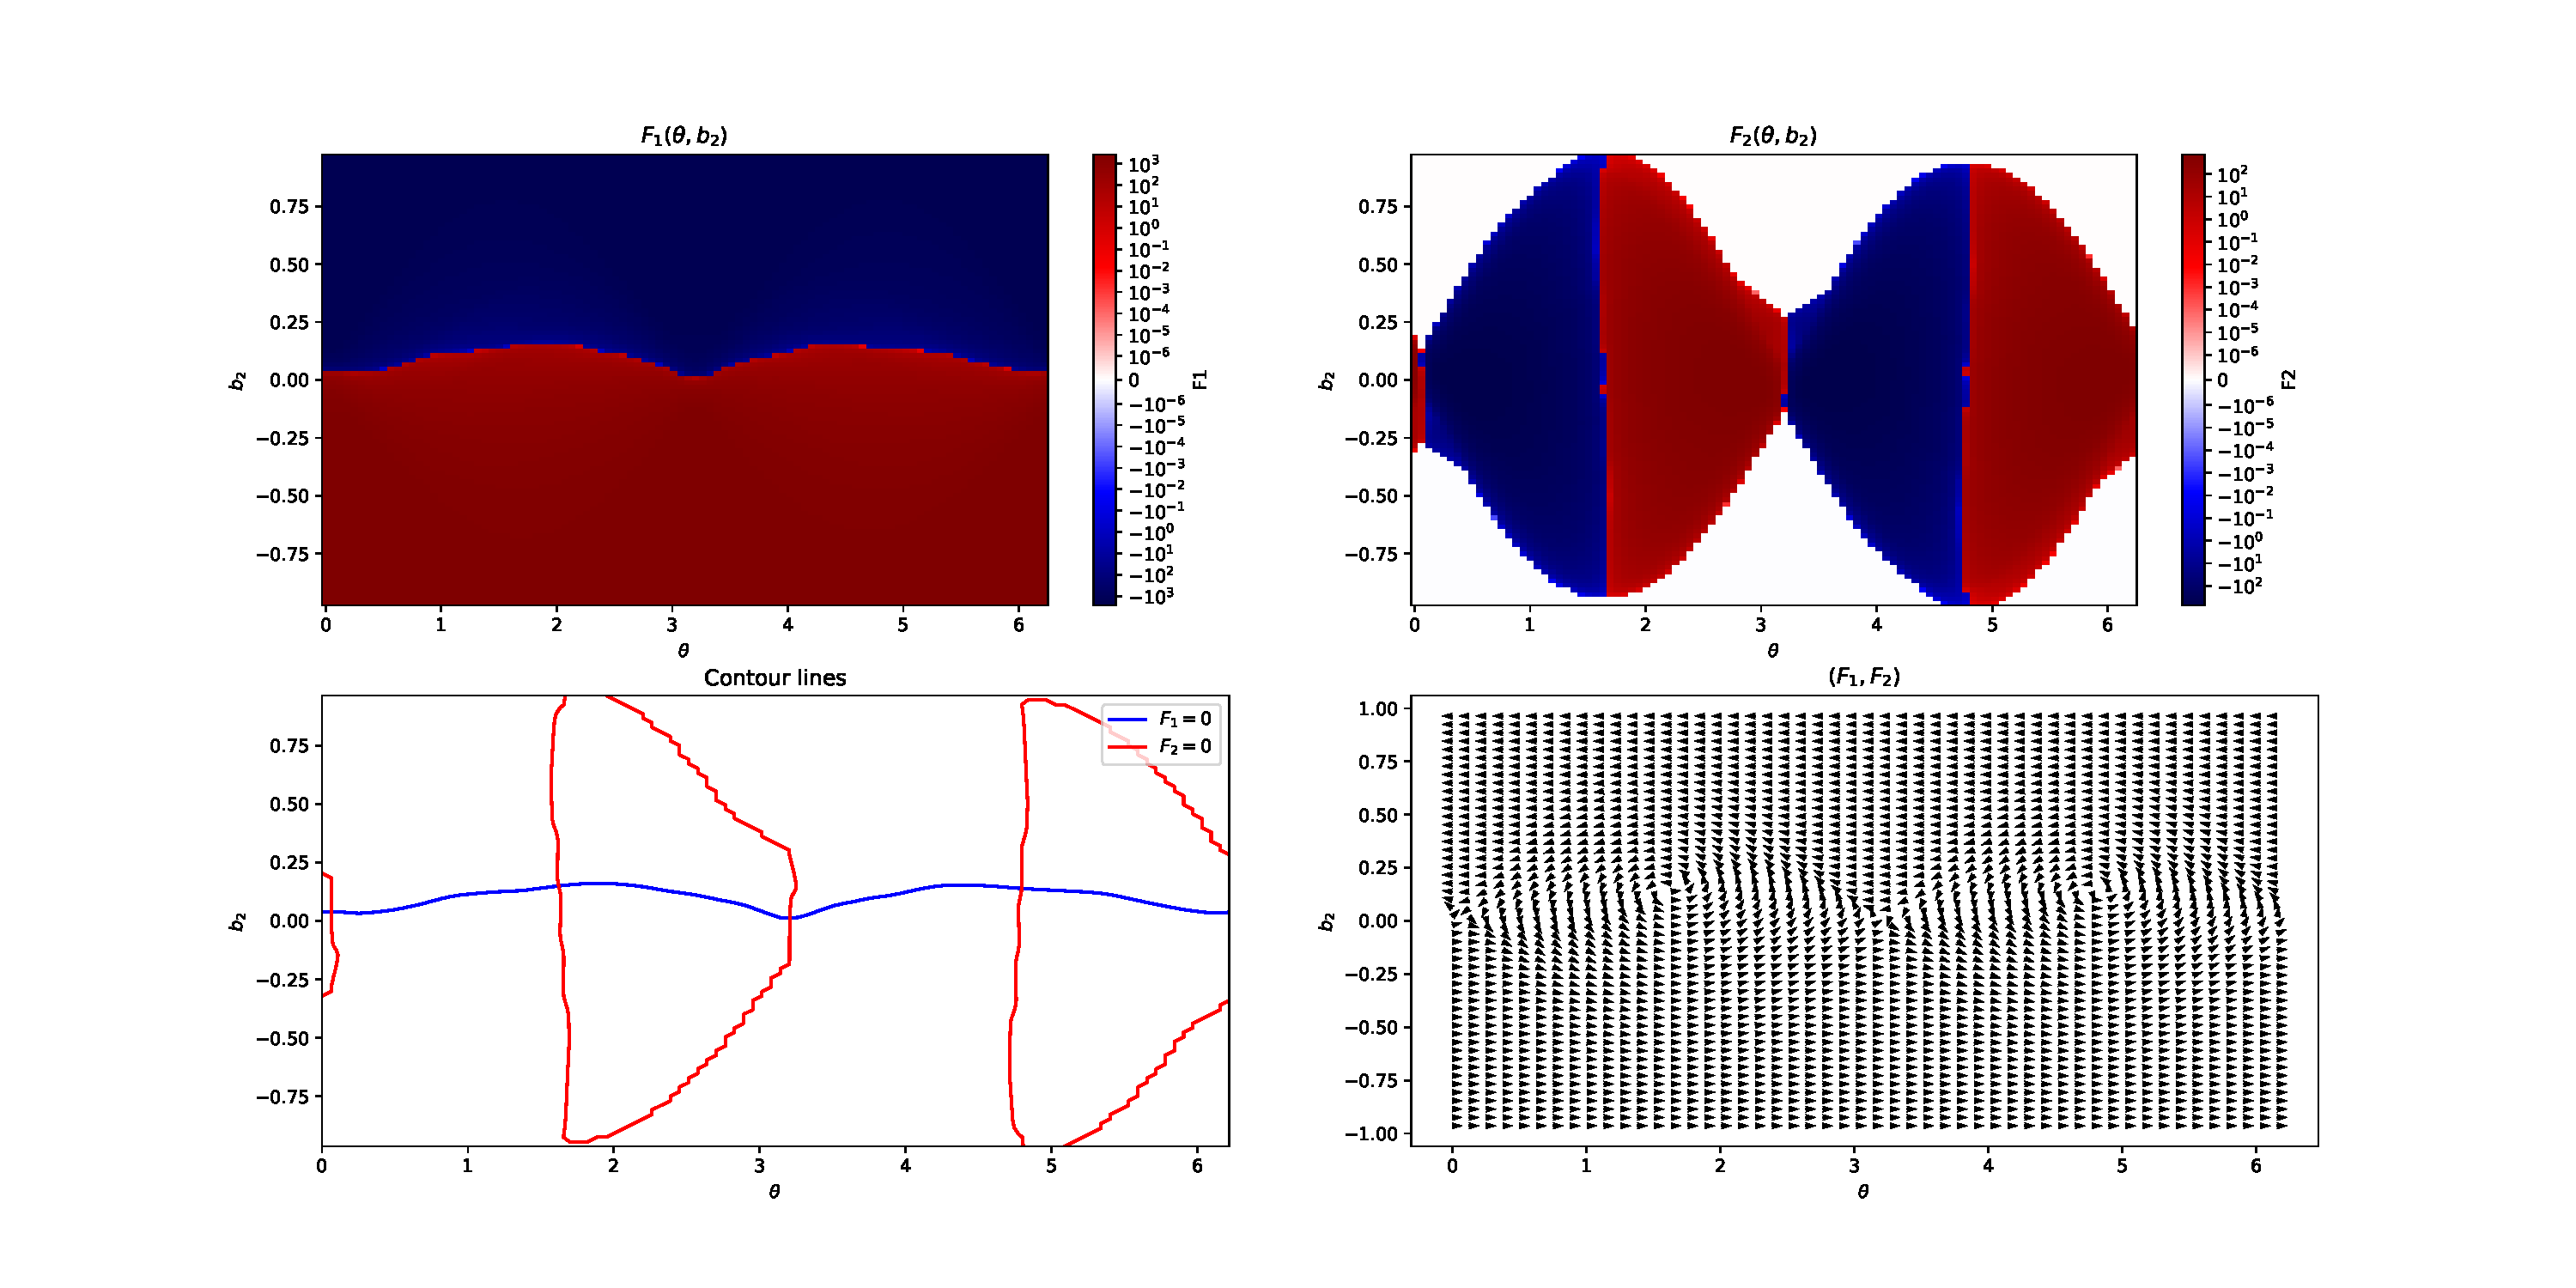
\includegraphics[width=\textwidth]{titanic/levels.pdf}
        \caption{Mapa de forças do Titanic}
        \label{fig:titanic_level}
    \end{figure}

    Novamente, o objeto possui 4 pontos de equilíbrio. As posições aproximadas desses pontos podem ser vistas na tabela \ref{table:titanic_approx}
    \begin{table}[H]
        \centering
        \begin{tabular}{ccc} \\

            
            \hline
            Índice do ponto & $\theta$ aproximado & $b_2$ aproximado \\

            \hline
            1 & 0.00 & 0.00 \\
            2 & $\pi/2$ & 0.00 \\
            3 & $\pi$ & 0.00 \\
            4 & $3\pi/2$ & 0.00 \\

            \hline
        \end{tabular}
        \caption{Aproximações dos pontos de equilíbrio do iceberg}
        \label{table:titanic_approx}
    \end{table} 

    Os pontos 2 e 4 são pontos de equilíbrio instável, enquanto a análise é inconclusiva para os pontos 1 e 3, pelo mesmo argumento utilizado na seção \ref{sec:ice_forca}. É visível que os mapas de forças são mais simples quando comparados aos mapas da figura \ref{fig:iceberg_level}, justificado por uma geometria mais regular.

    \subsubsection{Pontos de equilíbrio}
    Os pontos de equilíbrio encontrados são representados na figura \ref{fig:titanic_equi} e na tabela \ref{table:titanic_equi}.
    \begin{figure}[H]
        \centering
        \begin{subfigure}[b]{0.45\textwidth}
            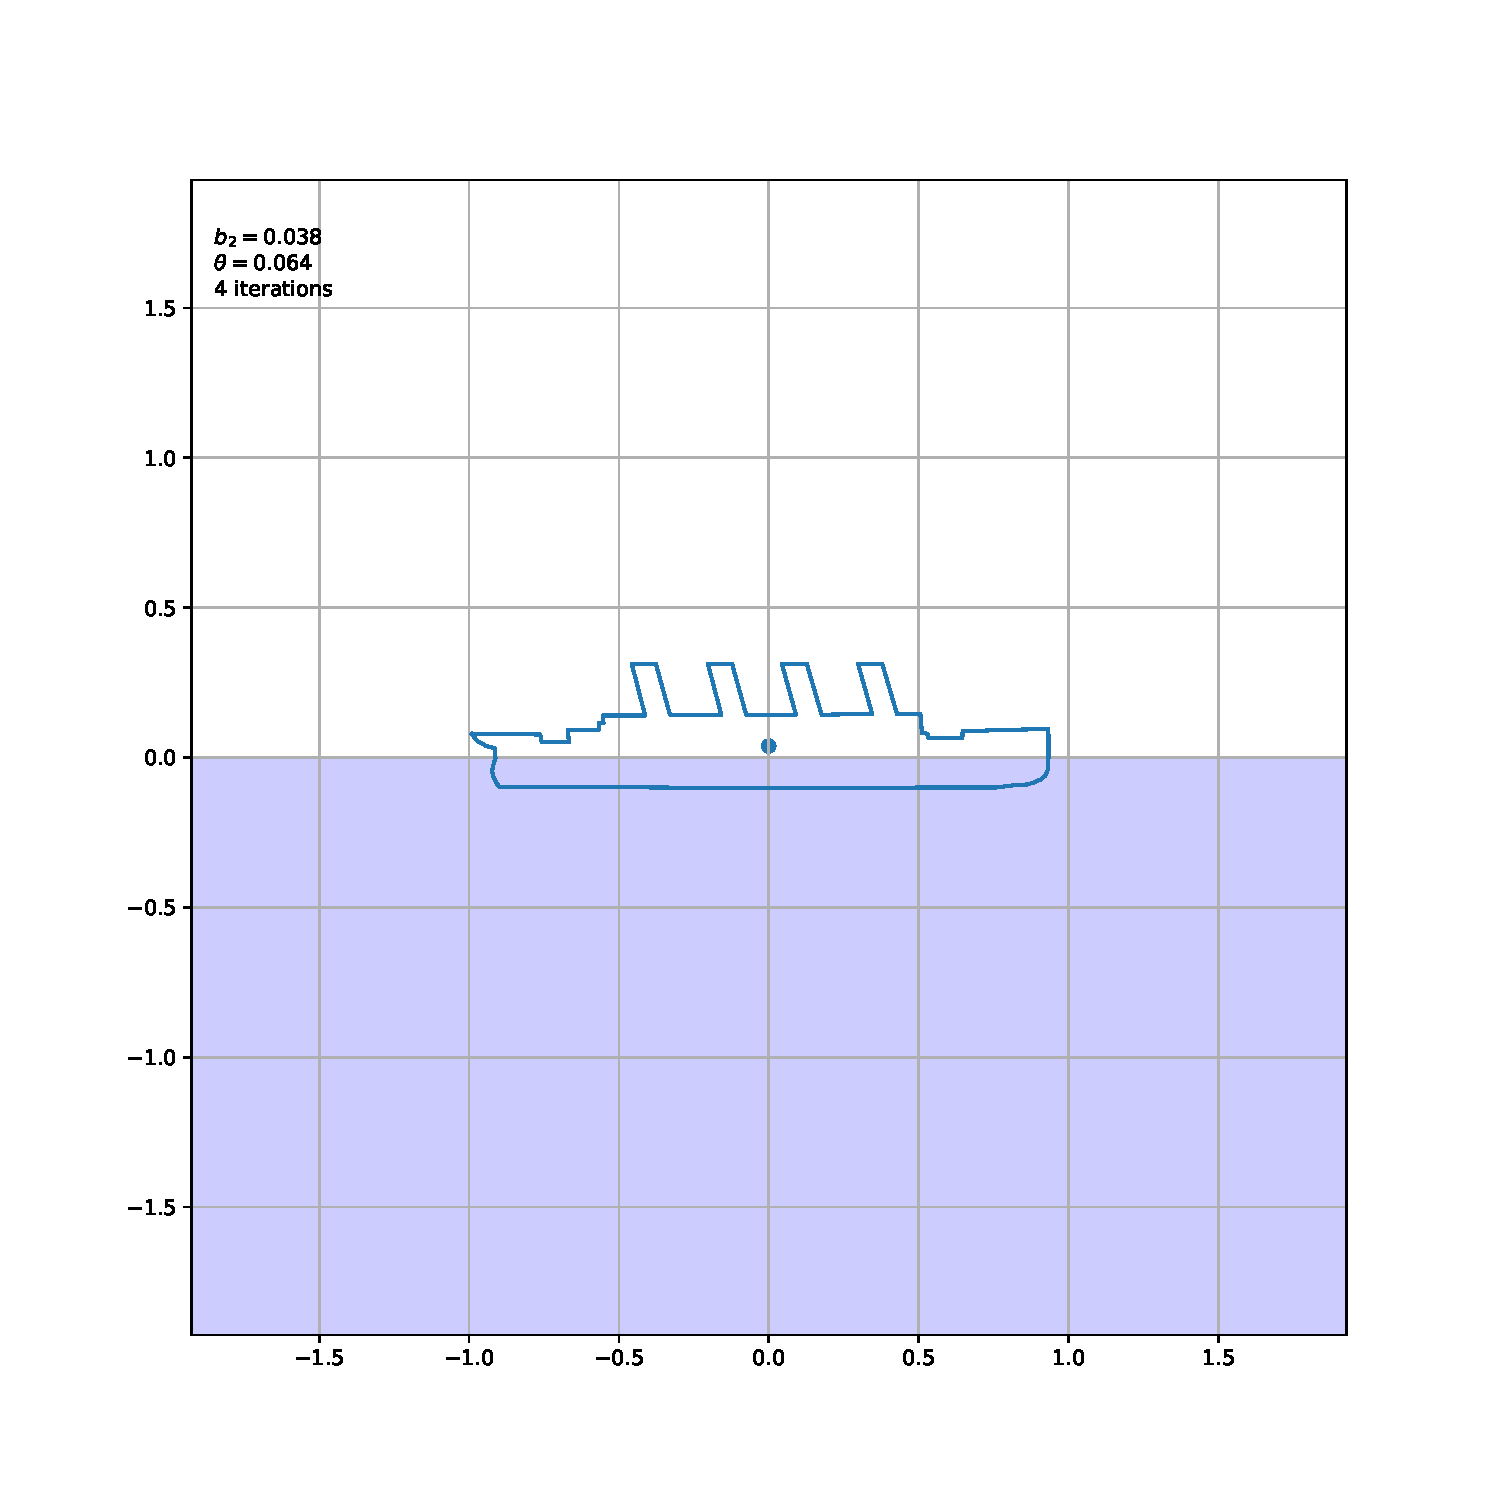
\includegraphics[width=\textwidth]{titanic/newton_b0=0.000_theta0=0.000.pdf}
            \caption{Partindo do ponto 1}    
        \end{subfigure}
        \quad
        \begin{subfigure}[b]{0.45\textwidth}
            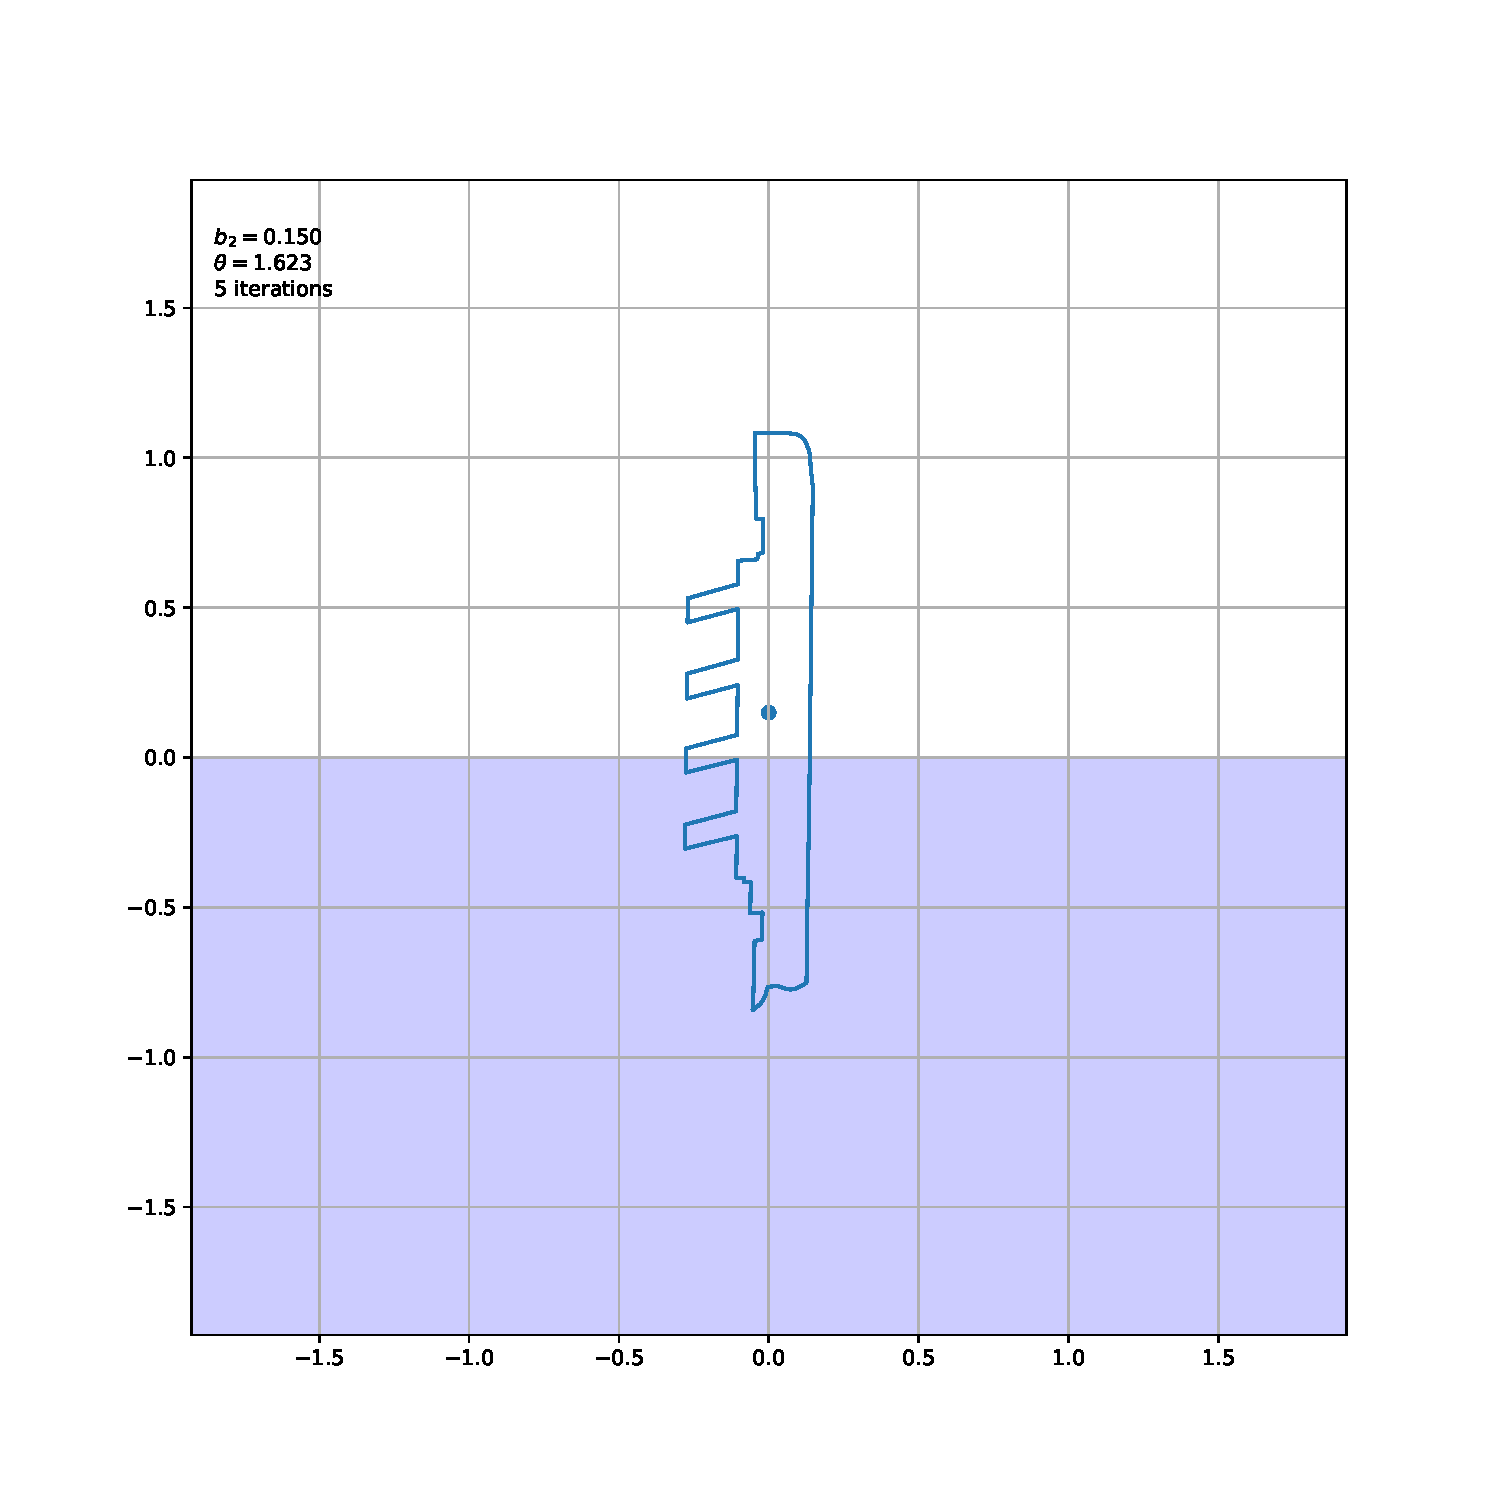
\includegraphics[width=\textwidth]{titanic/newton_b0=0.000_theta0=1.571.pdf}    
            \caption{Partindo do ponto 2}
        \end{subfigure}
        \quad
        \begin{subfigure}[b]{0.45\textwidth}
            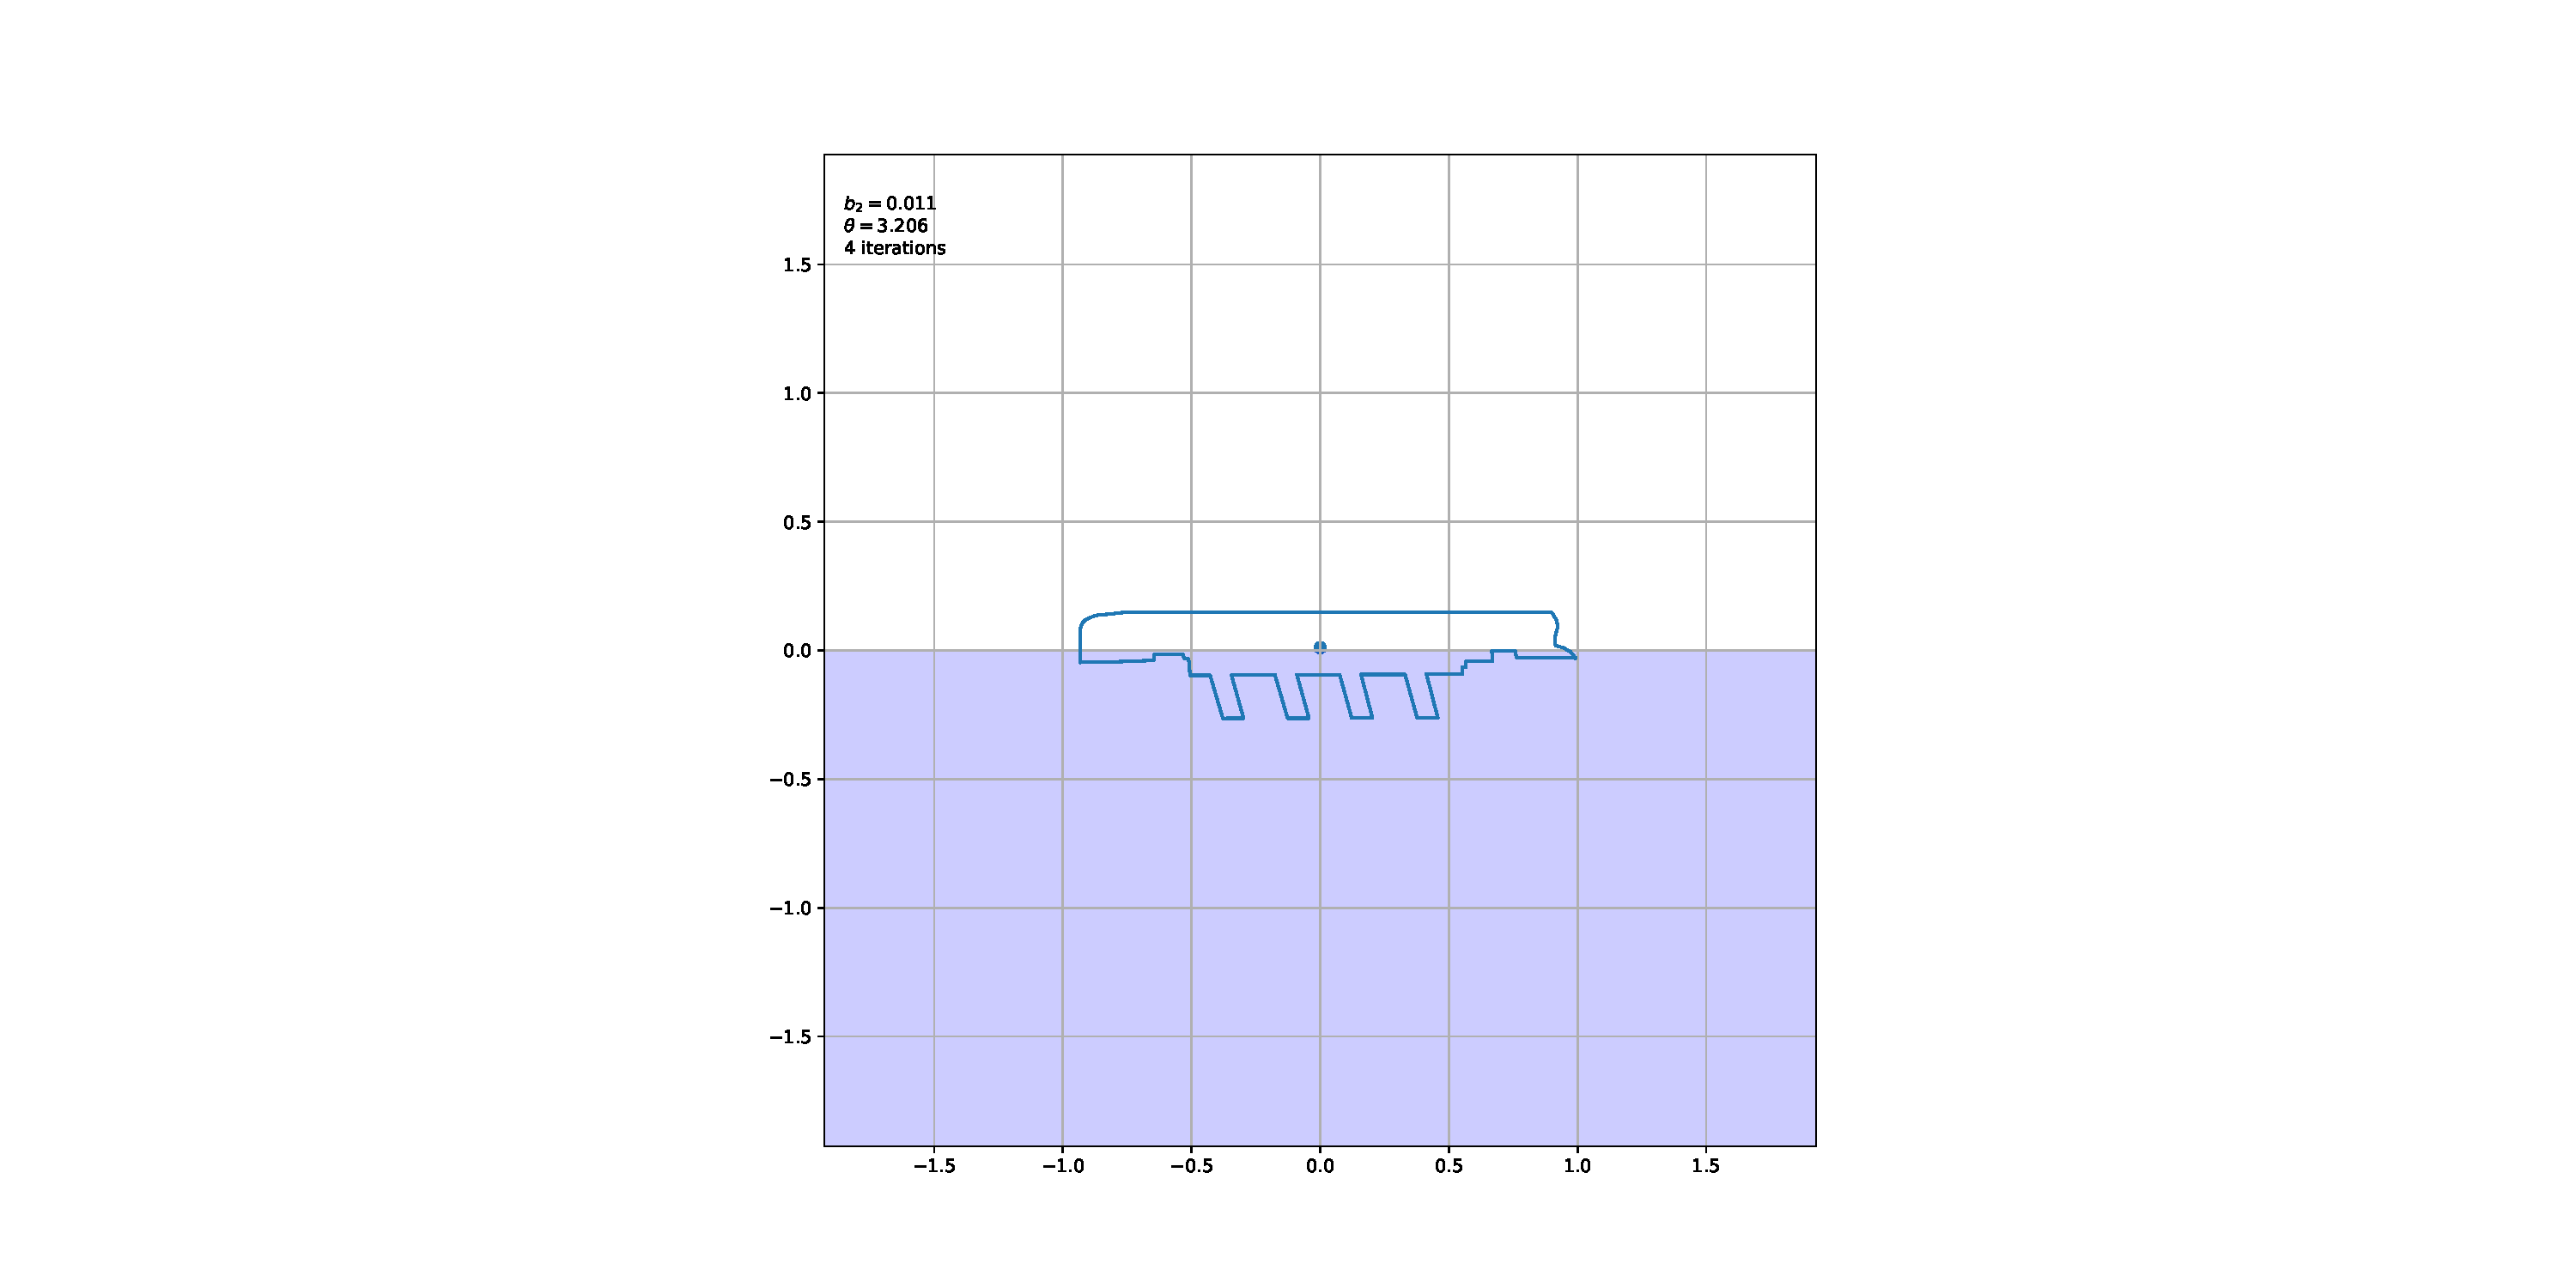
\includegraphics[width=\textwidth]{titanic/newton_b0=0.000_theta0=3.142.pdf}
            \caption{Partindo do ponto 3}    
        \end{subfigure}
        \quad
        \begin{subfigure}[b]{0.45\textwidth}
            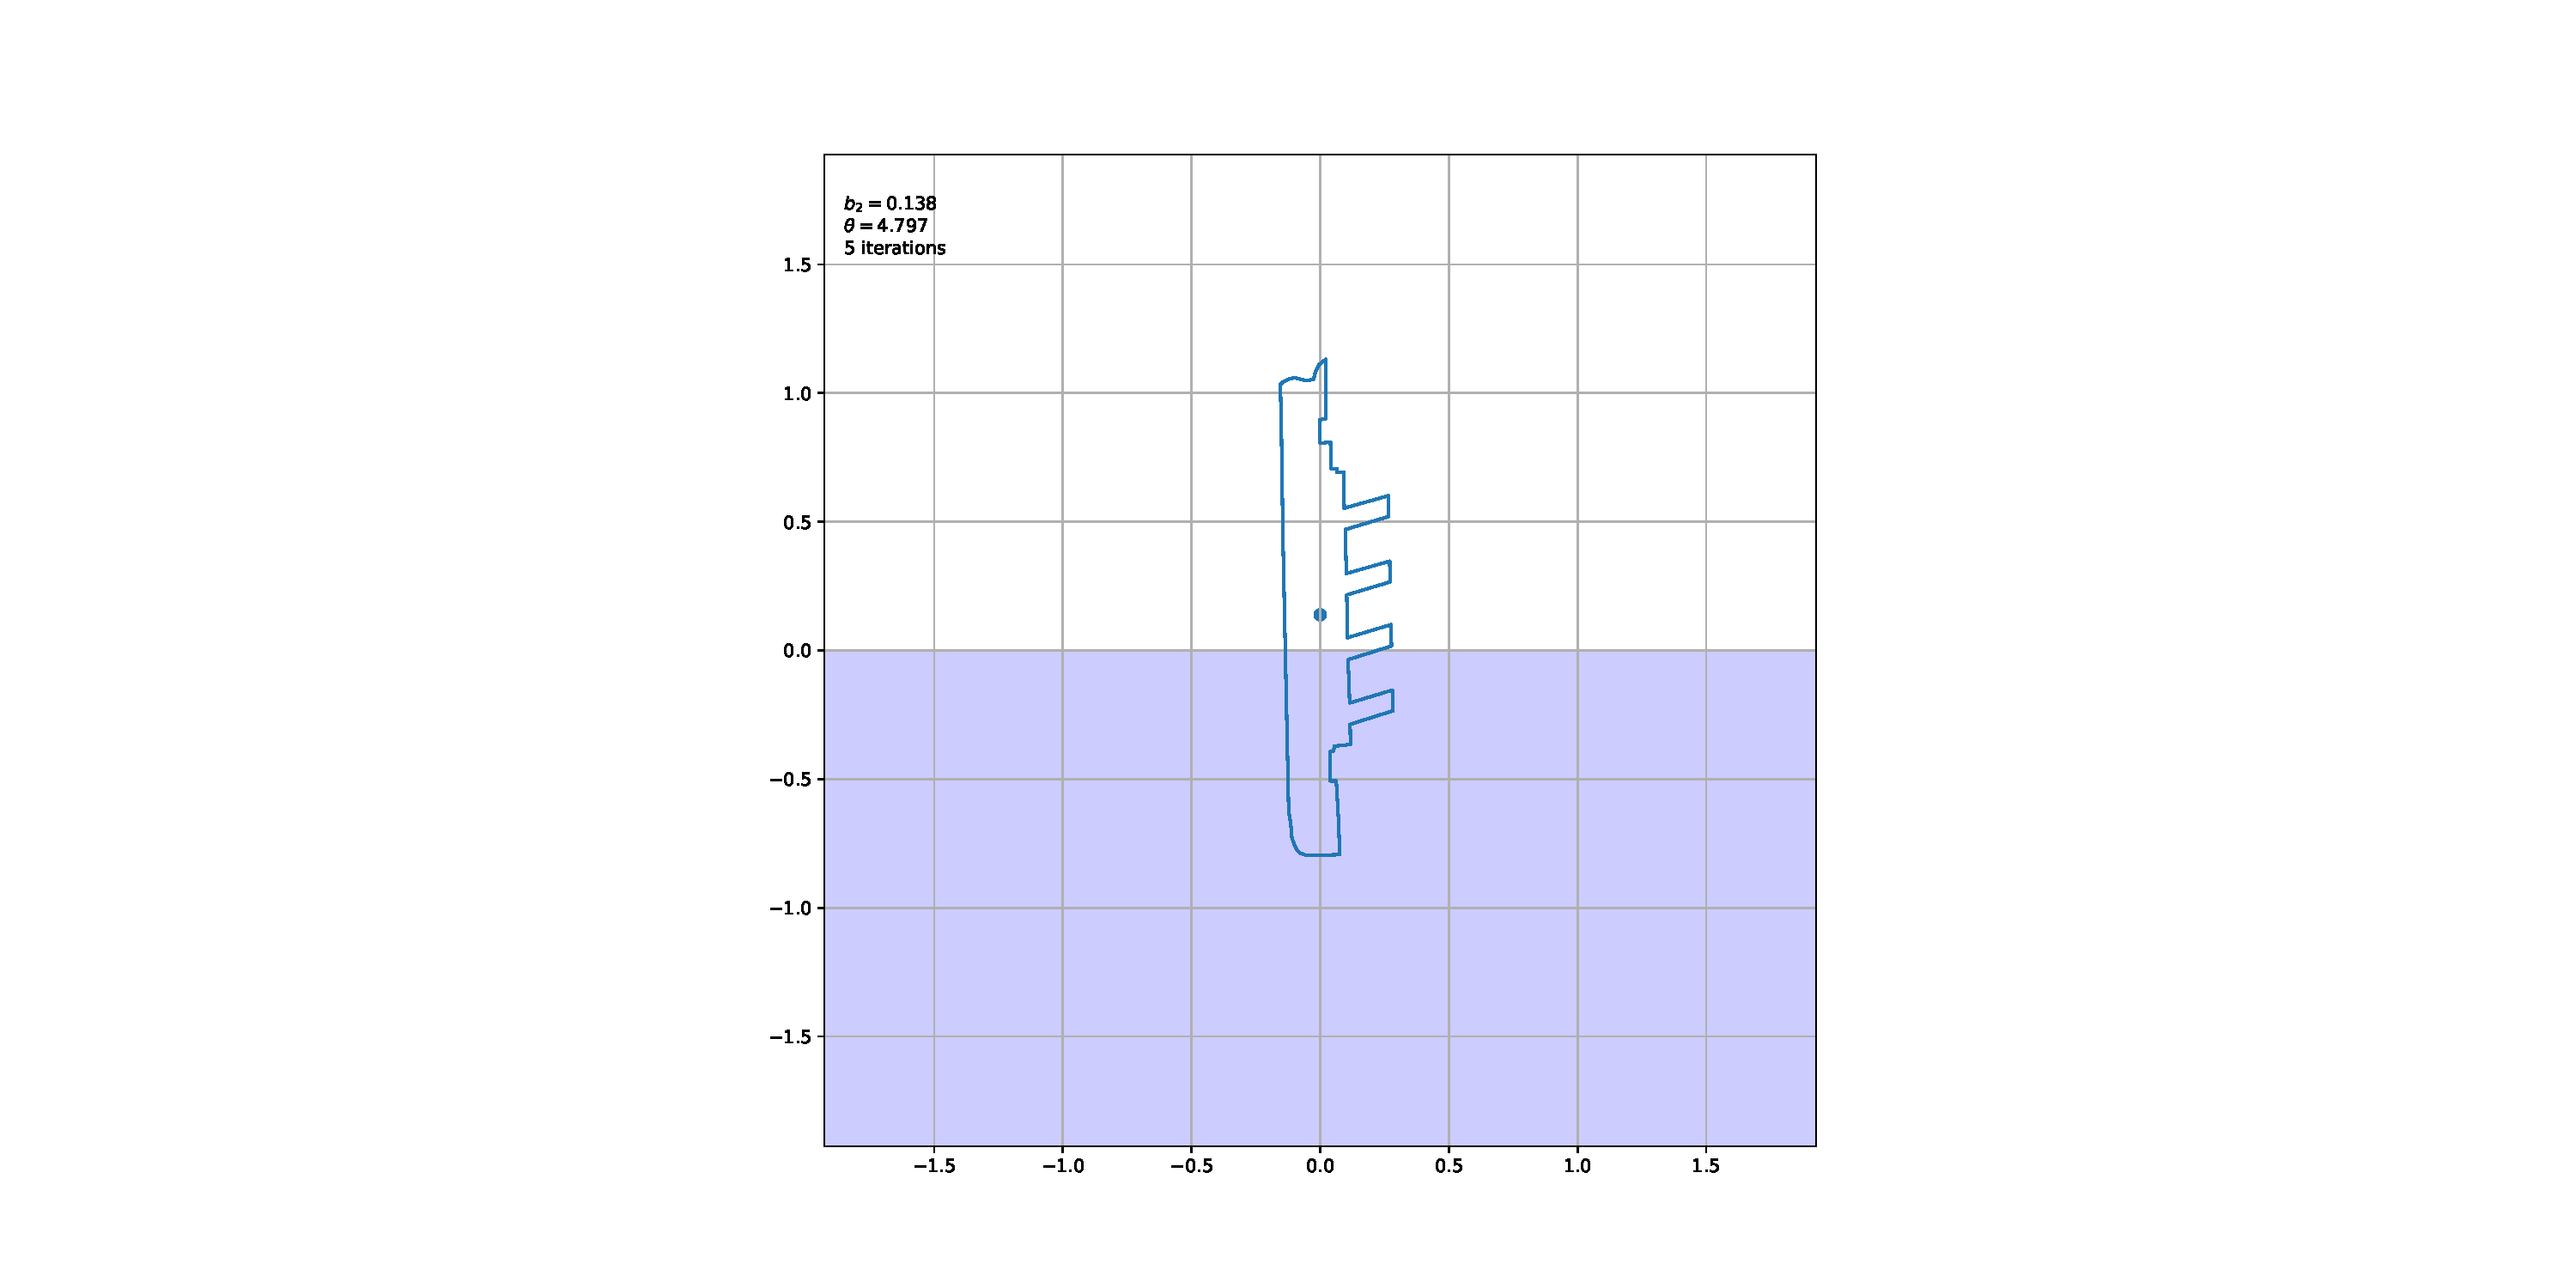
\includegraphics[width=\textwidth]{titanic/newton_b0=0.000_theta0=4.712.pdf}
            \caption{Partindo do ponto 4}    
        \end{subfigure}
        \quad
        
        \caption{Pontos de equilíbrio encontrados para o Titanic}
        \label{fig:titanic_equi}
    \end{figure}
    
    \begin{table}[H]
        \centering
        \begin{tabular}{ccccc} \\

            
            \hline
            Índice & $\theta$ & $b_2$ & Iterações & Ordem média de convergência \\

            \hline
            1 & 0.064 & 0.038  & 4 & 3.077\\
            2 & 1.623 & 0.150 & 5 & 2.134\\
            3 & 3.206 & 0.011 & 4 & 2.147\\
            4 & 4.797 & 0.138 & 5 & 1.938 \\

            \hline
        \end{tabular}
        \caption{Pontos de equilíbrio encontrados para o Titanic}
        \label{table:titanic_equi}
    \end{table}

    A convergência tem ordem aproximada quadrática para esse caso, o que significa que os pontos iniciais escolhidos estão bons o suficiente.

    \FloatBarrier
    \subsubsection{Análise dinâmica}

    Como a densidade do objeto é $400 kg/m^3$, o objeto começa a subir, porém em pouca quantidade (na ordem de $1e-1$ de grandeza). Devido à sua regularidade (se assemelha a um retângulo), somado com a baixa "energia" inicial, o comportamento nos diversos casos é semelhante, mudando apenas o tempo em que o corpo entra em estado estacionário de flutuação. Isso fica claro nas Figuras \ref{fig:titanic_PVI1}, \ref{fig:titanic_PVI2} e \ref{fig:titanic_PVI3}. Em todos os casos que chegaram num estado estacionário, a solução convergiu para o ponto 1.

    Ademais, foi testada a convergência do método empregado para resolver o PVI para o Titanic, como pode ser visto nas Figuras \ref{fig:titanic_conv1} e \ref{fig:titanic_conv2}. Para esses casos, foi utilizado $c_1 =1$ e $c_2 = 1$.
    
    É possível ver, na figura \ref{fig:titanic_conv2} que a curva de convergência se assemelha muito à curva $O(h^4)$. Porém, existe algum trecho em que a ordem de convergência se afasta de 4 no intervalo $[0.125, 0.25]$.

    Devido à natureza fortemente oscilatória da solução, passos de tempo muito grandes quebram a simulação, como observado na figura \ref{fig:titanic_conv1} para o passo de tempo $h=0.5$.

    \begin{figure}
        \centering
        \begin{subfigure}[b]{0.9\textwidth}
            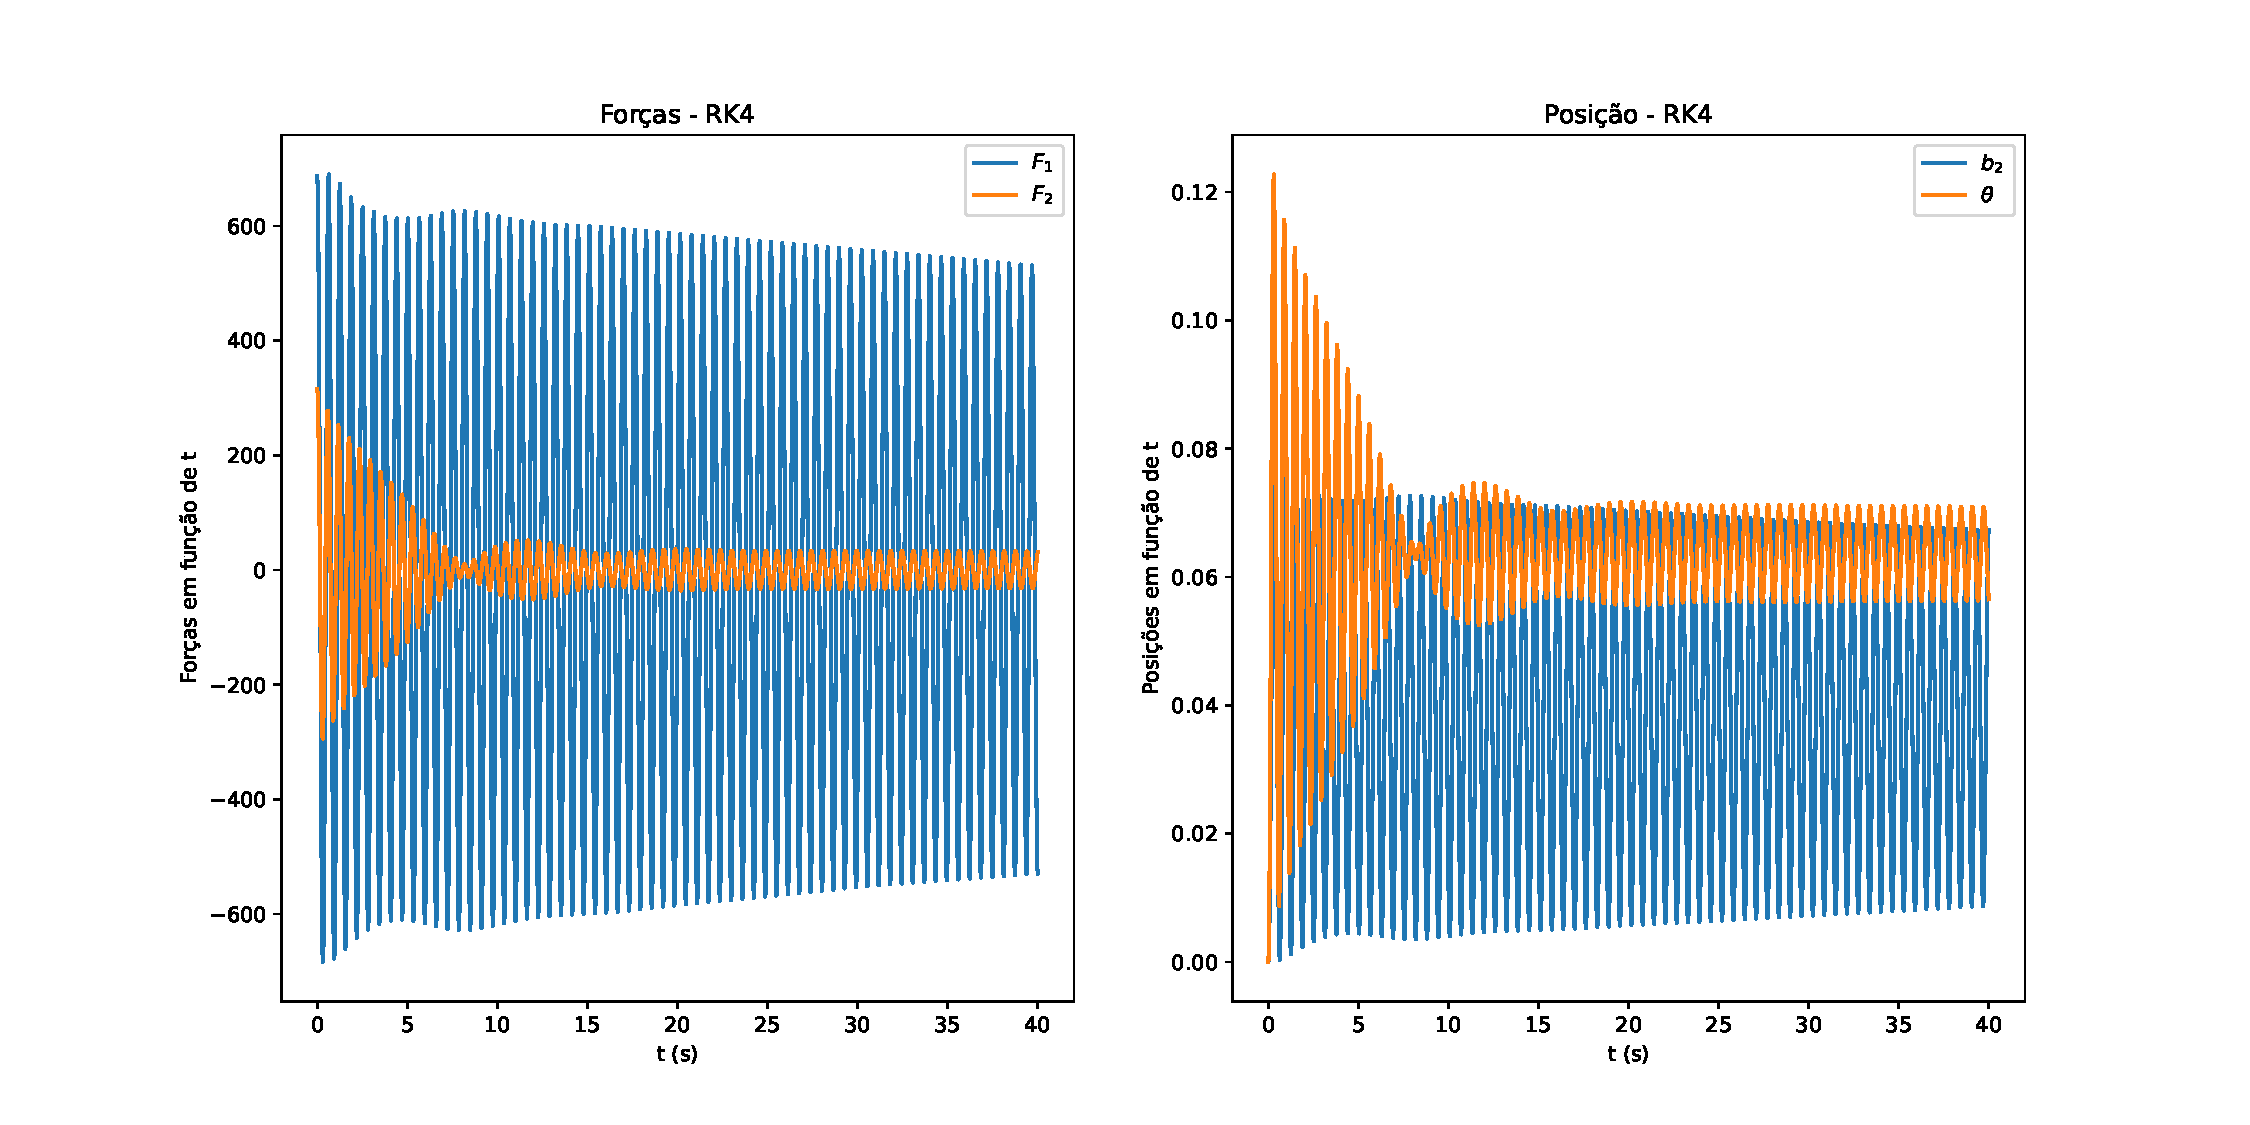
\includegraphics[width=\textwidth]{titanic/PVI_h=0.03_g1=1.0_g2=0.5.pdf}
            \caption{$\gamma_2 = 0.5$}
        \end{subfigure}
        \quad
        \begin{subfigure}[b]{0.9\textwidth}
            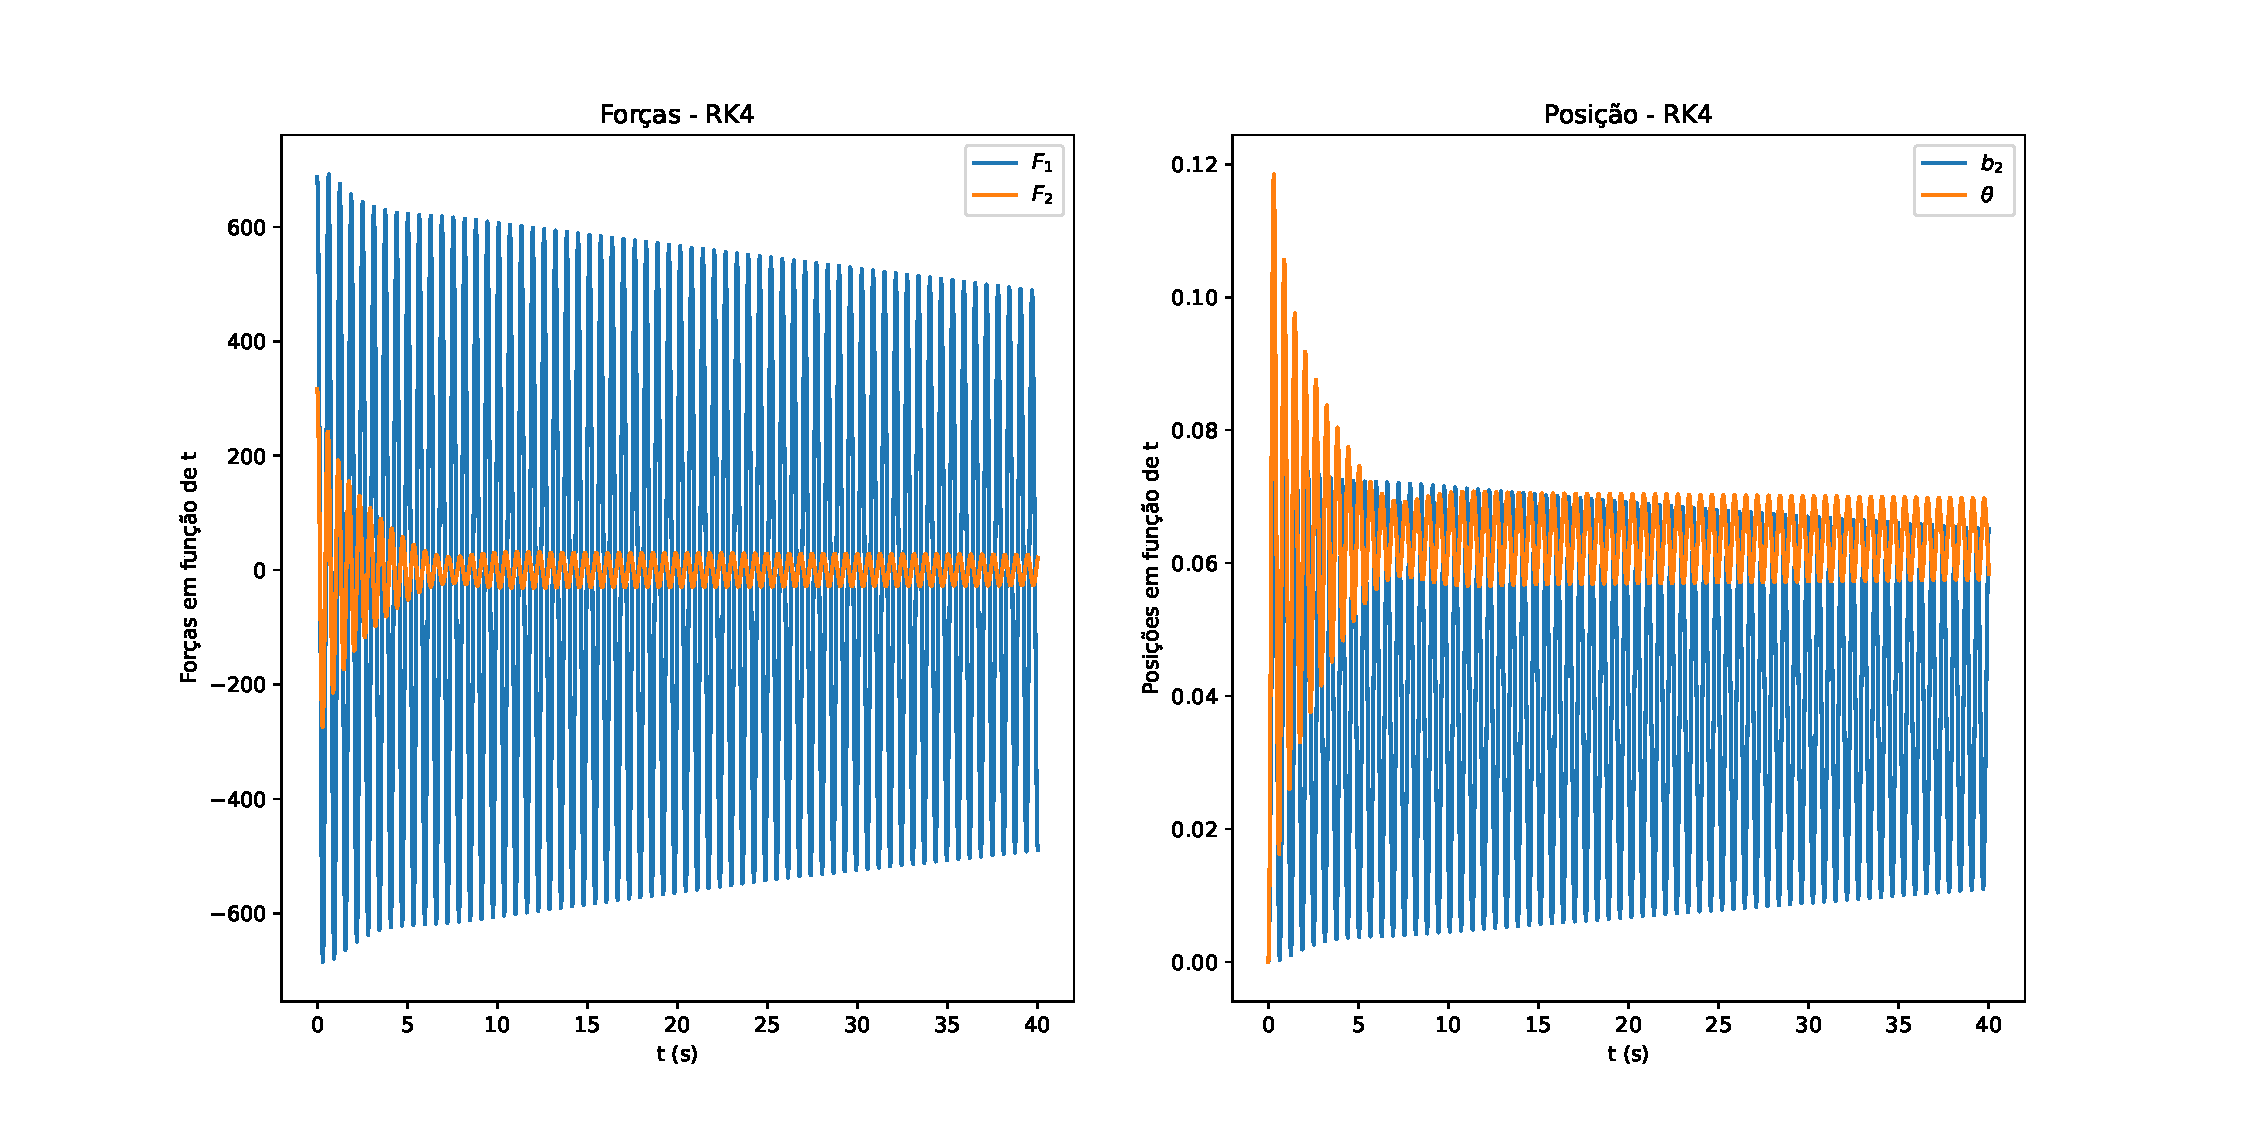
\includegraphics[width=\textwidth]{titanic/PVI_h=0.03_g1=1.0_g2=1.0.pdf}
            \caption{$\gamma_2 = 1.0$}
        \end{subfigure}
        \quad
        \begin{subfigure}[b]{0.9\textwidth}
            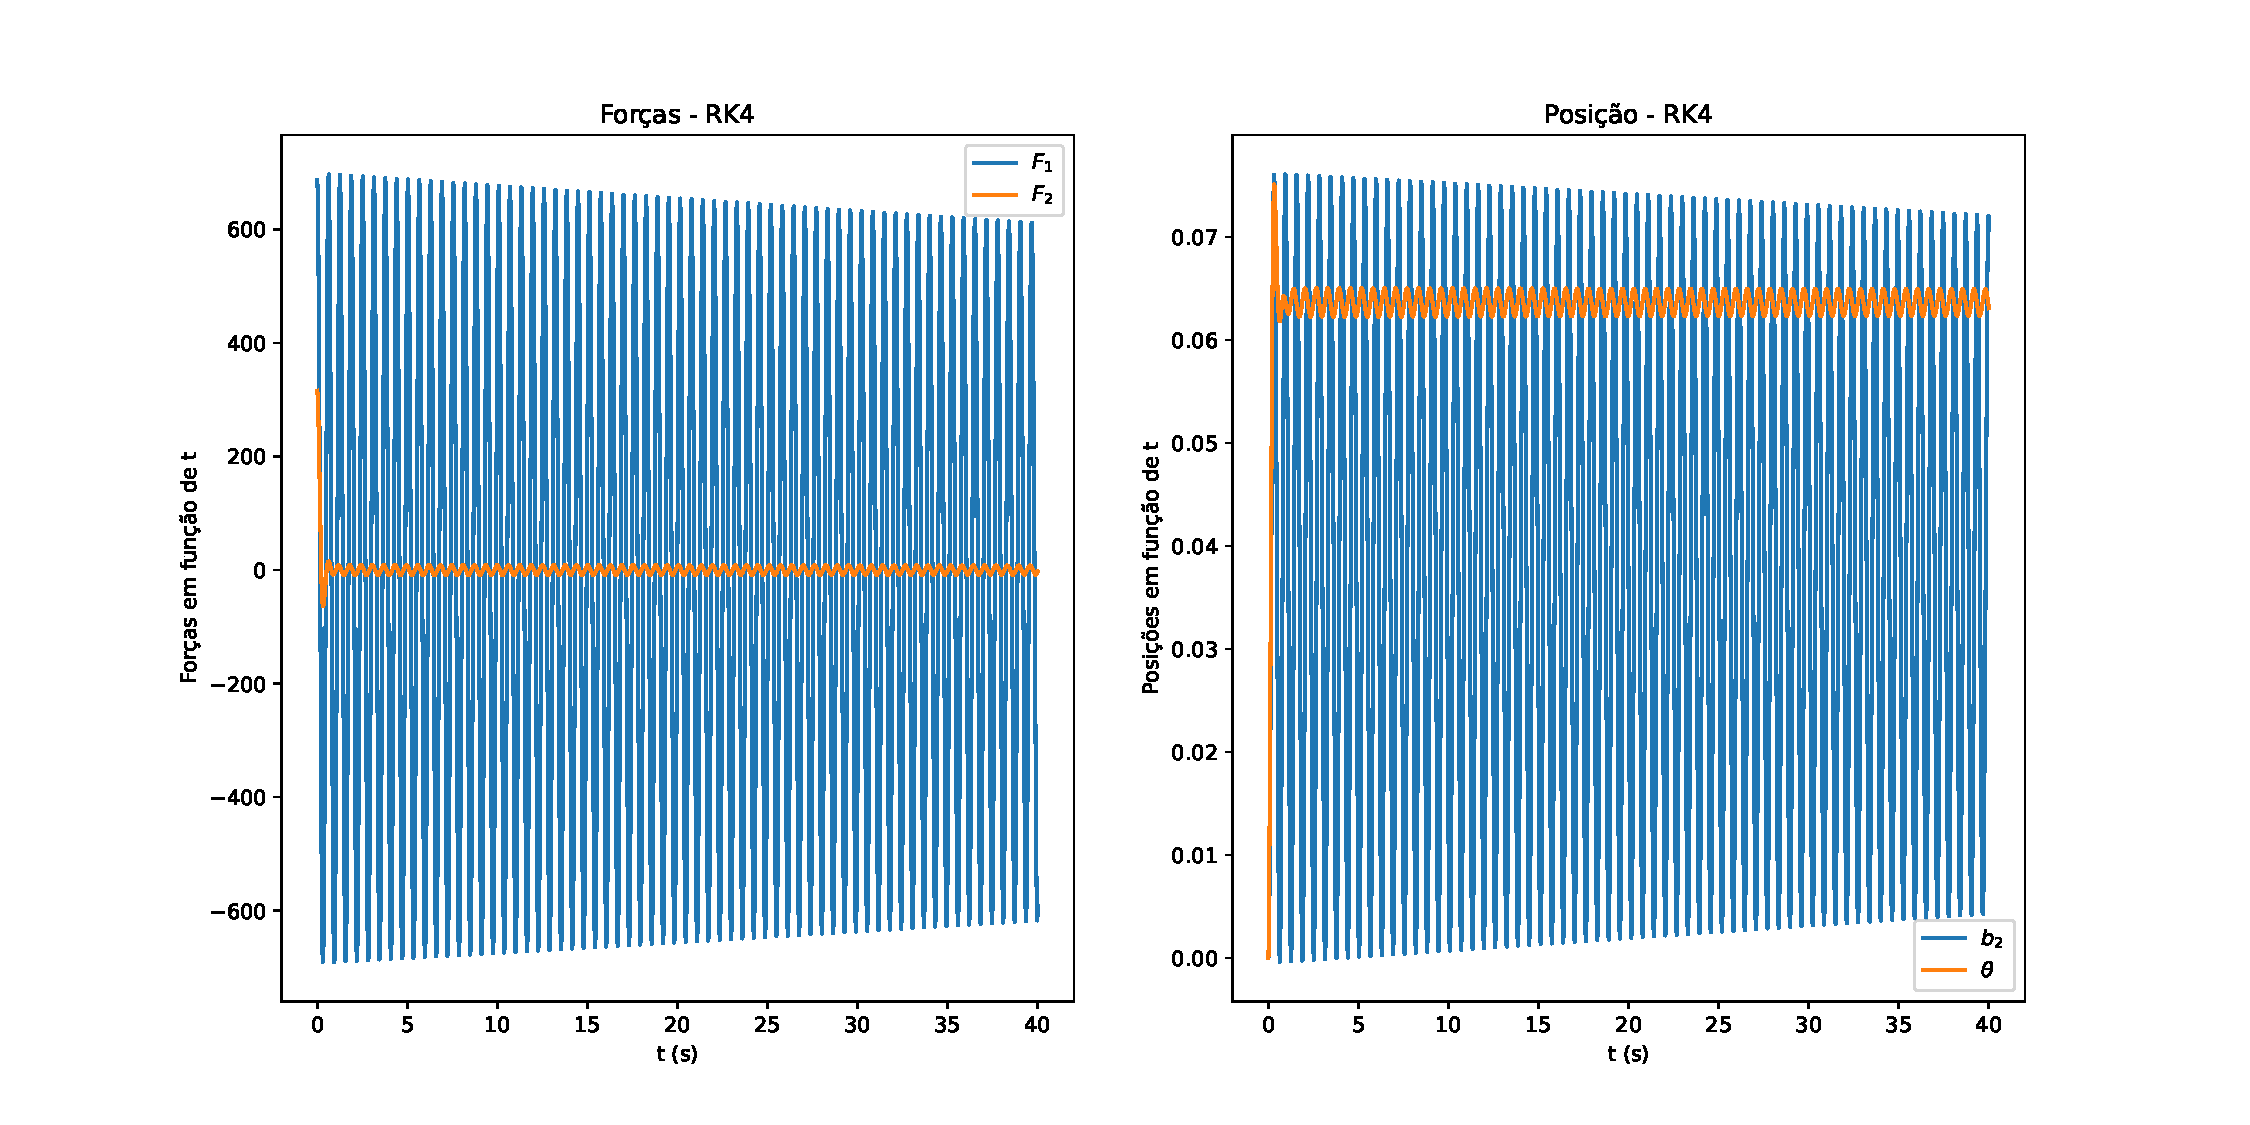
\includegraphics[width=\textwidth]{titanic/PVI_h=0.03_g1=1.0_g2=10.0.pdf}
            \caption{$\gamma_2 = 10.0$}
        \end{subfigure}
        \caption{PVI com $\gamma_1 = 1.0$ (Titanic)}
        \label{fig:titanic_PVI1}
    \end{figure}

    \begin{figure}
        \centering
        \begin{subfigure}[b]{0.9\textwidth}
            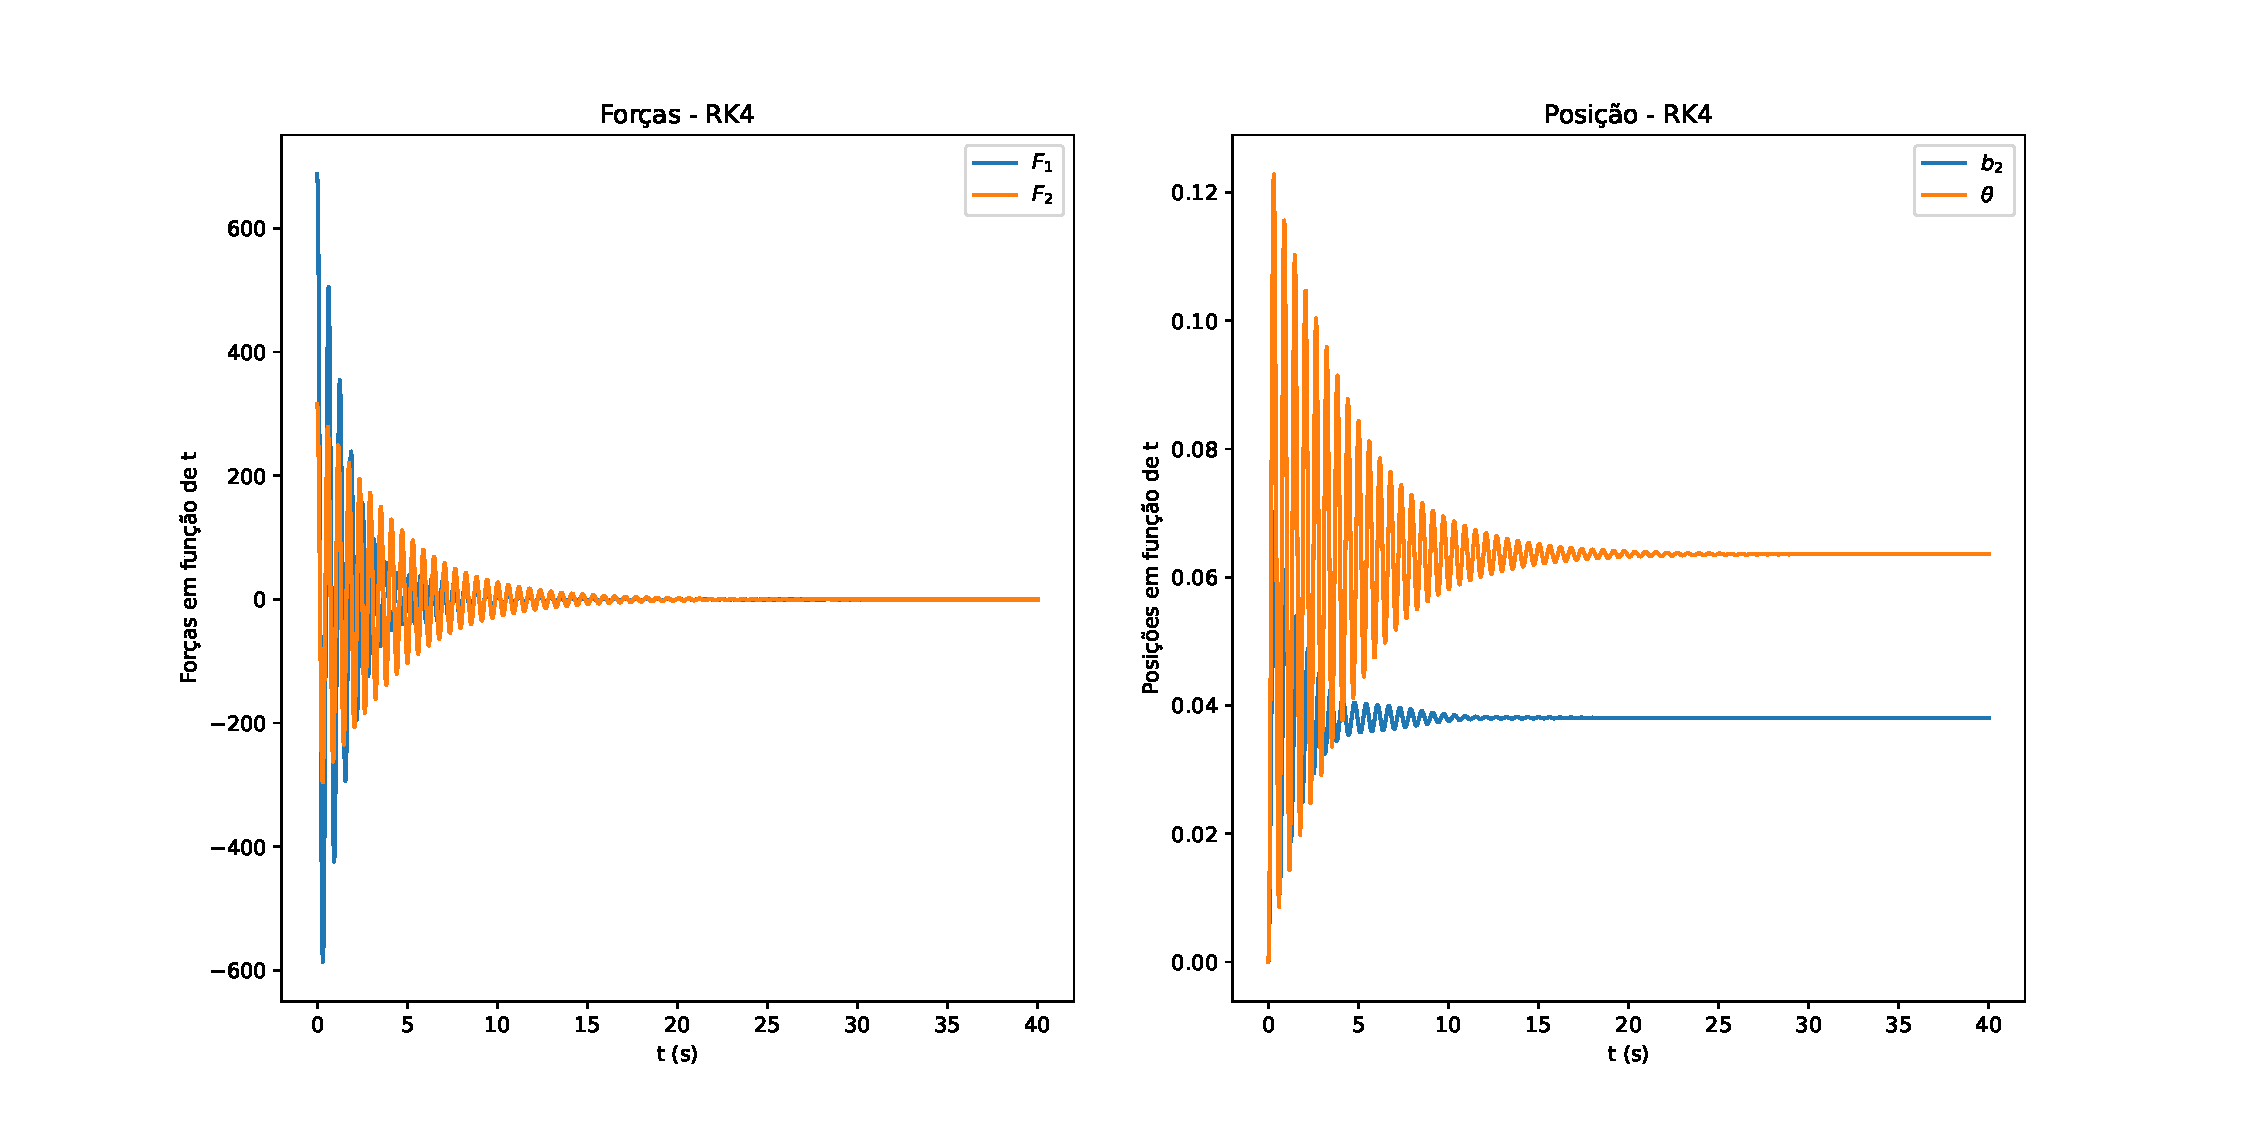
\includegraphics[width=\textwidth]{titanic/PVI_h=0.03_g1=400.0_g2=0.5.pdf}
            \caption{$\gamma_2 = 0.5$}
        \end{subfigure}
        \quad
        \begin{subfigure}[b]{0.9\textwidth}
            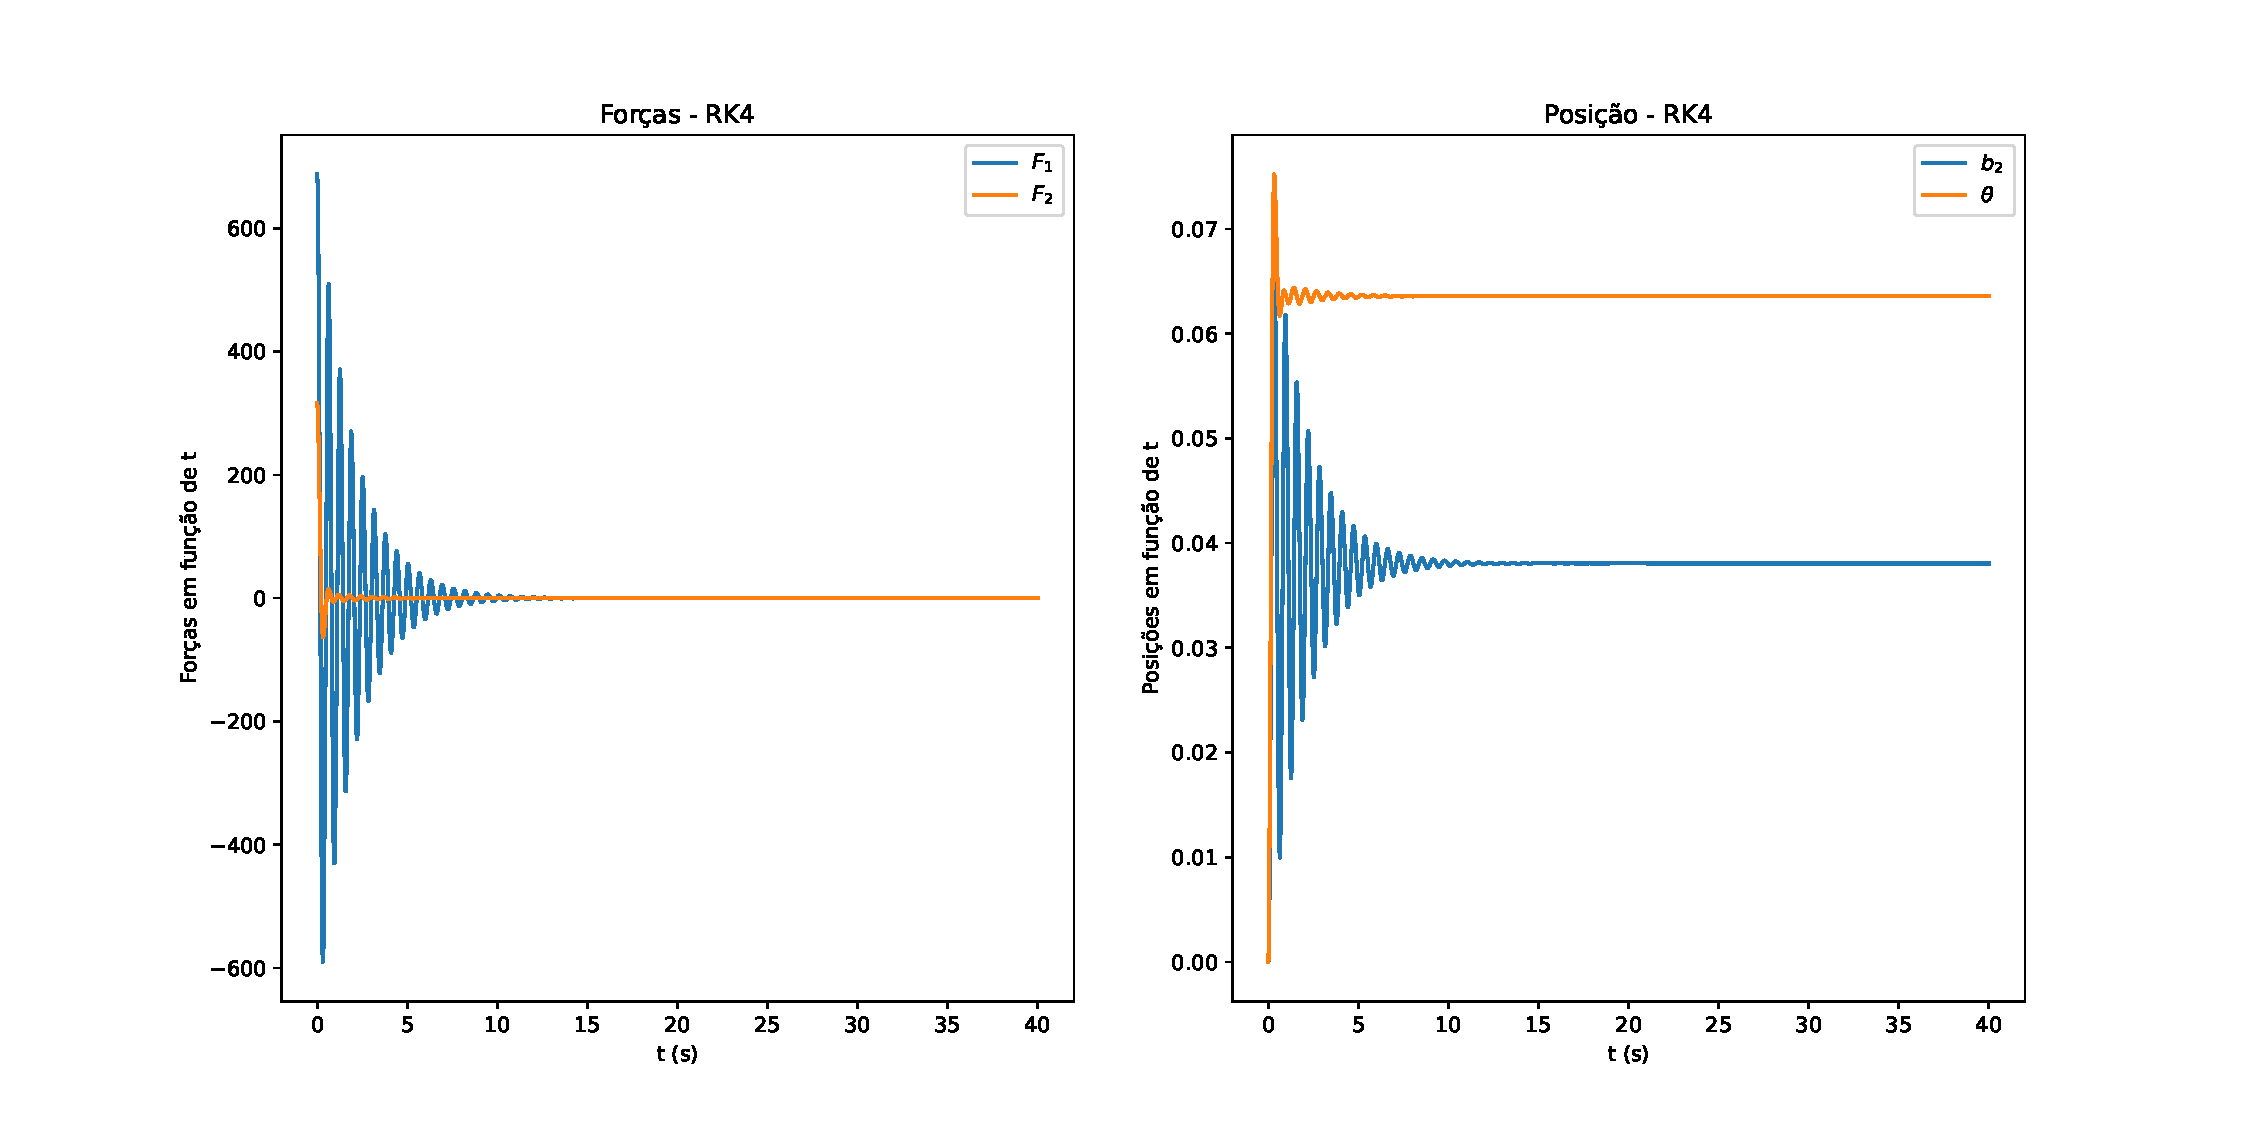
\includegraphics[width=\textwidth]{titanic/PVI_h=0.03_g1=400.0_g2=10.0.pdf}
            \caption{$\gamma_2 = 1.0$}
        \end{subfigure}
        \quad
        \begin{subfigure}[b]{0.9\textwidth}
            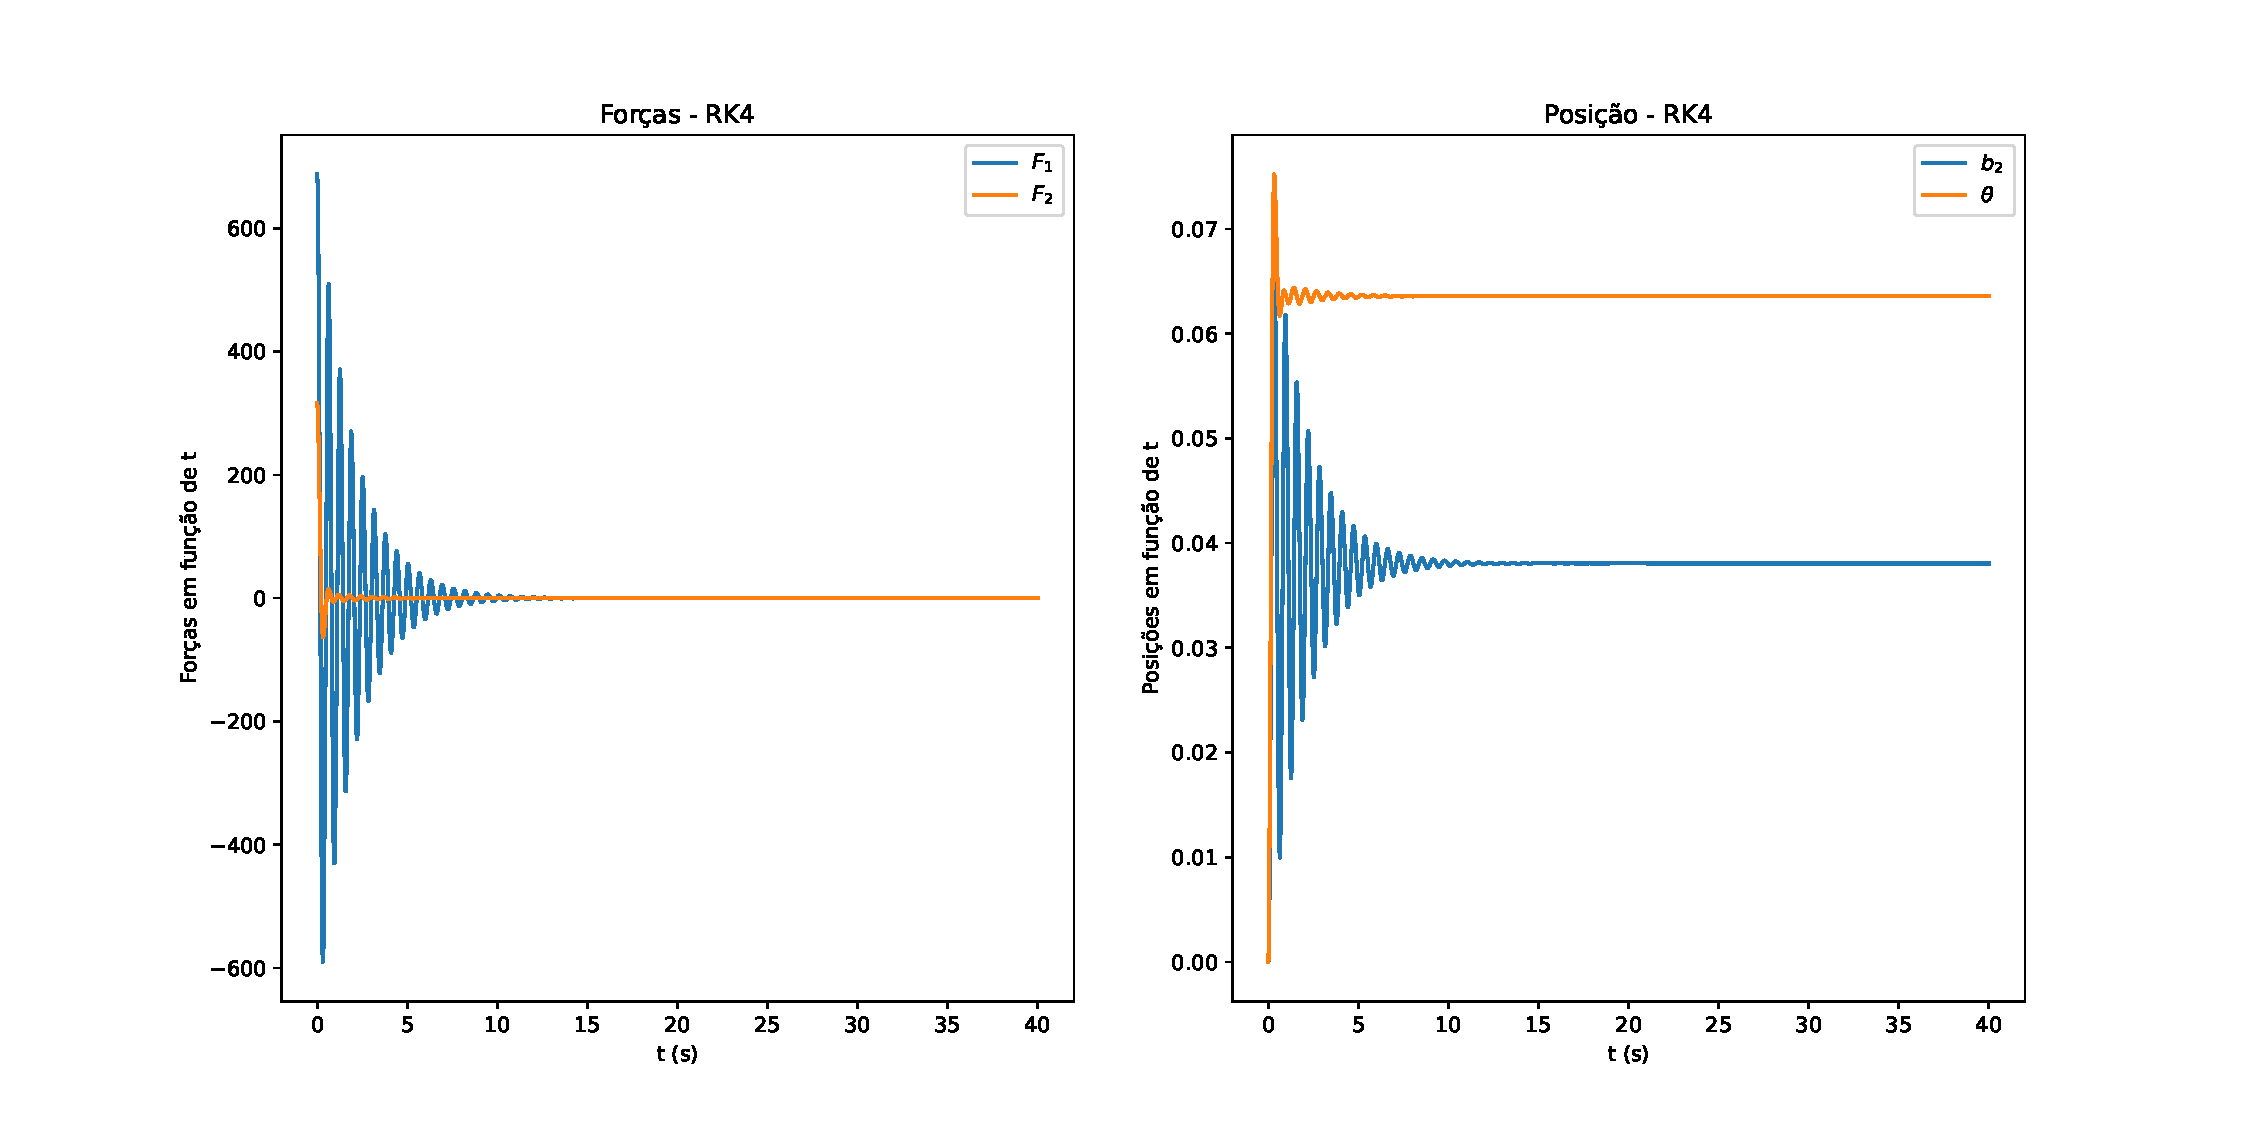
\includegraphics[width=\textwidth]{titanic/PVI_h=0.03_g1=400.0_g2=10.0.pdf}
            \caption{$\gamma_2 = 10.0$}
        \end{subfigure}
        \caption{PVI com $\gamma_1 = 400.0$ (Titanic)}
        \label{fig:titanic_PVI2}
    \end{figure}

    \begin{figure}
        \centering
        \begin{subfigure}[b]{0.9\textwidth}
            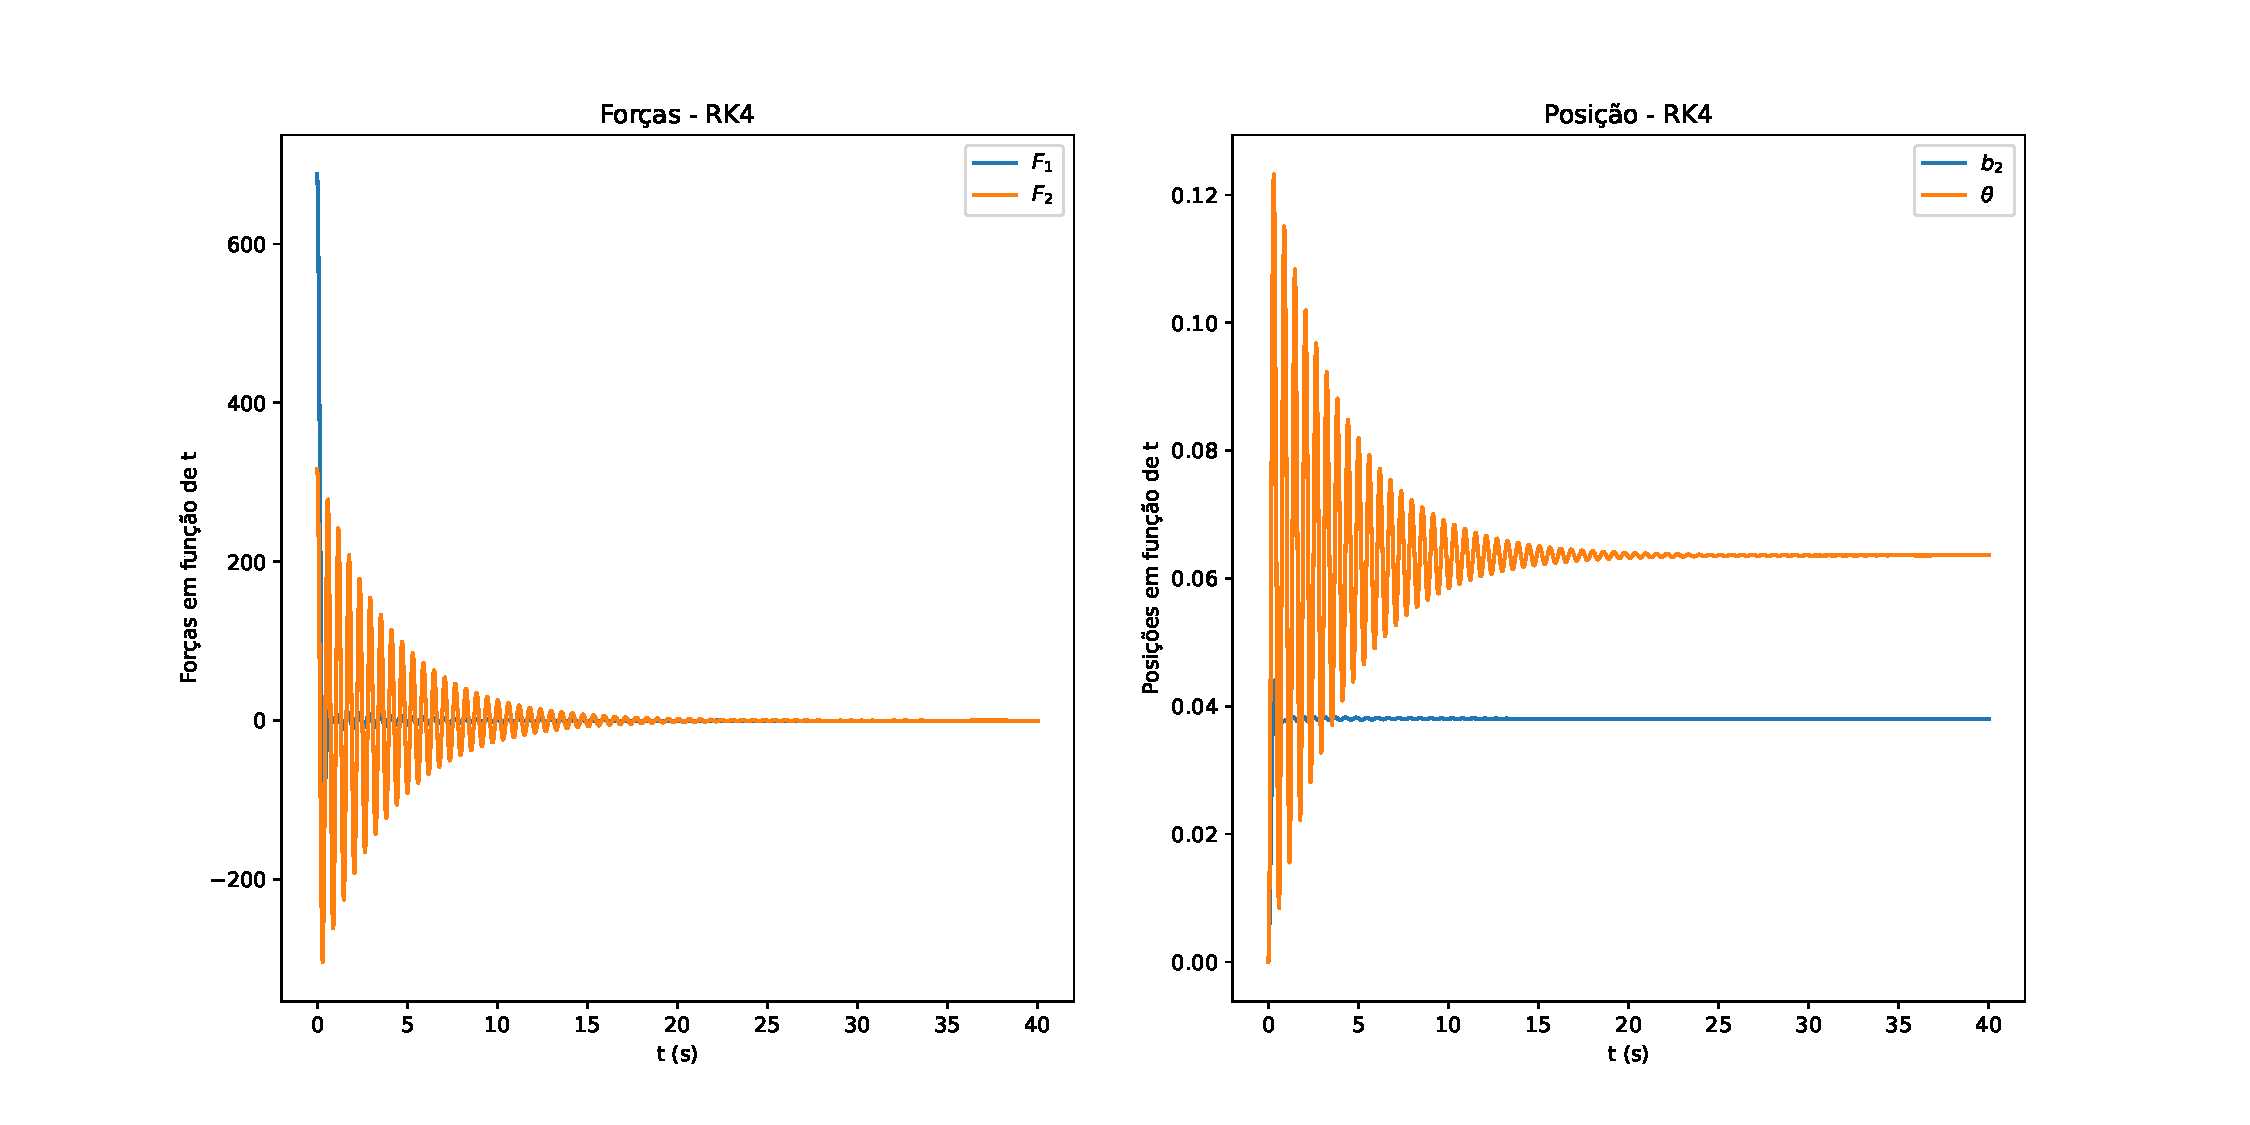
\includegraphics[width=\textwidth]{titanic/PVI_h=0.03_g1=4000.0_g2=0.5.pdf}
            \caption{$\gamma_2 = 0.5$}
        \end{subfigure}
        \quad
        \begin{subfigure}[b]{0.9\textwidth}
            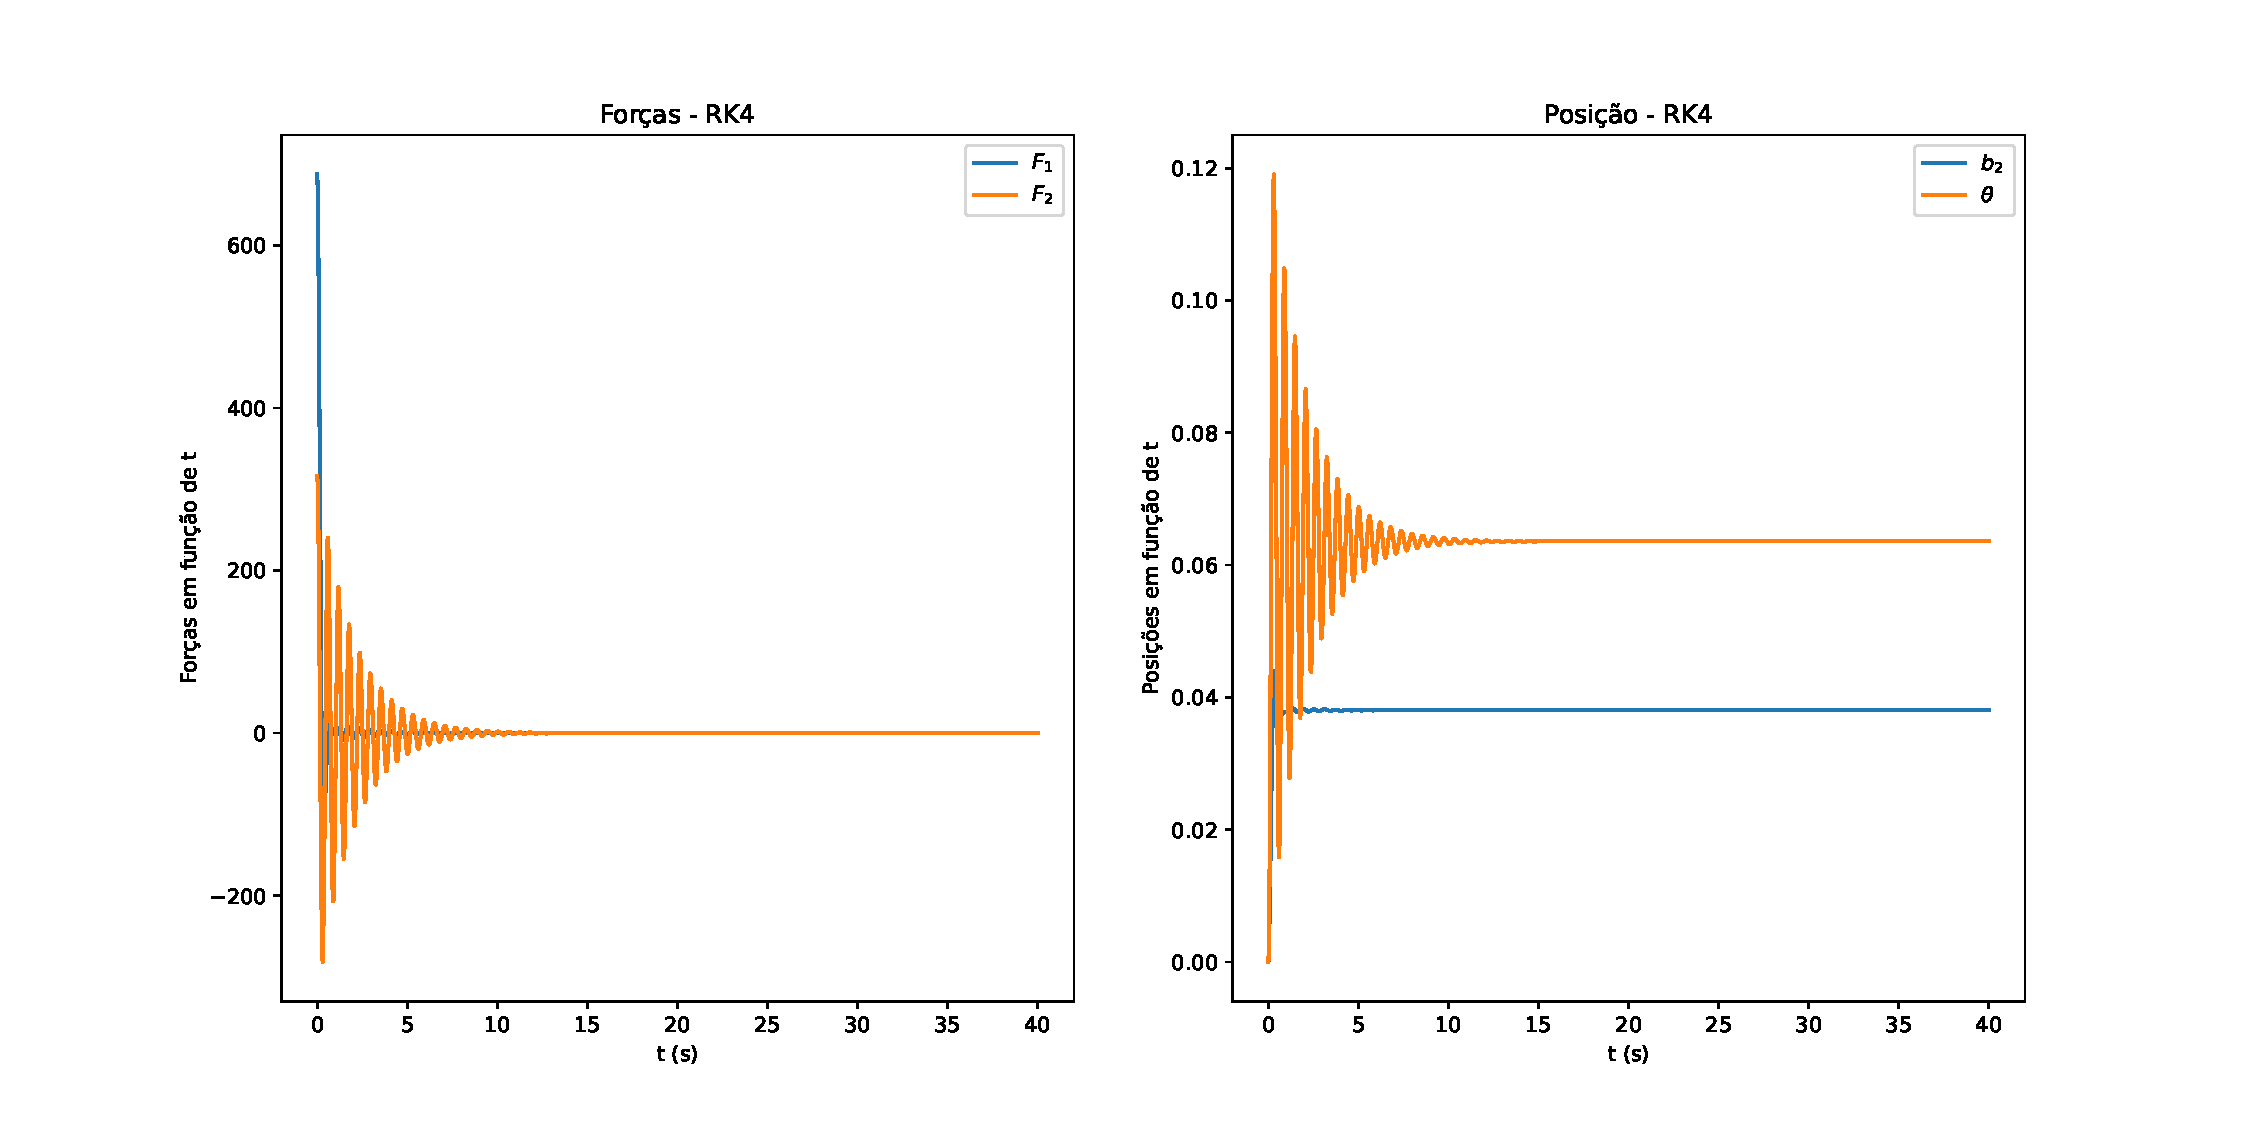
\includegraphics[width=\textwidth]{titanic/PVI_h=0.03_g1=4000.0_g2=1.0.pdf}
            \caption{$\gamma_2 = 1.0$}
        \end{subfigure}
        \quad
        \begin{subfigure}[b]{0.9\textwidth}
            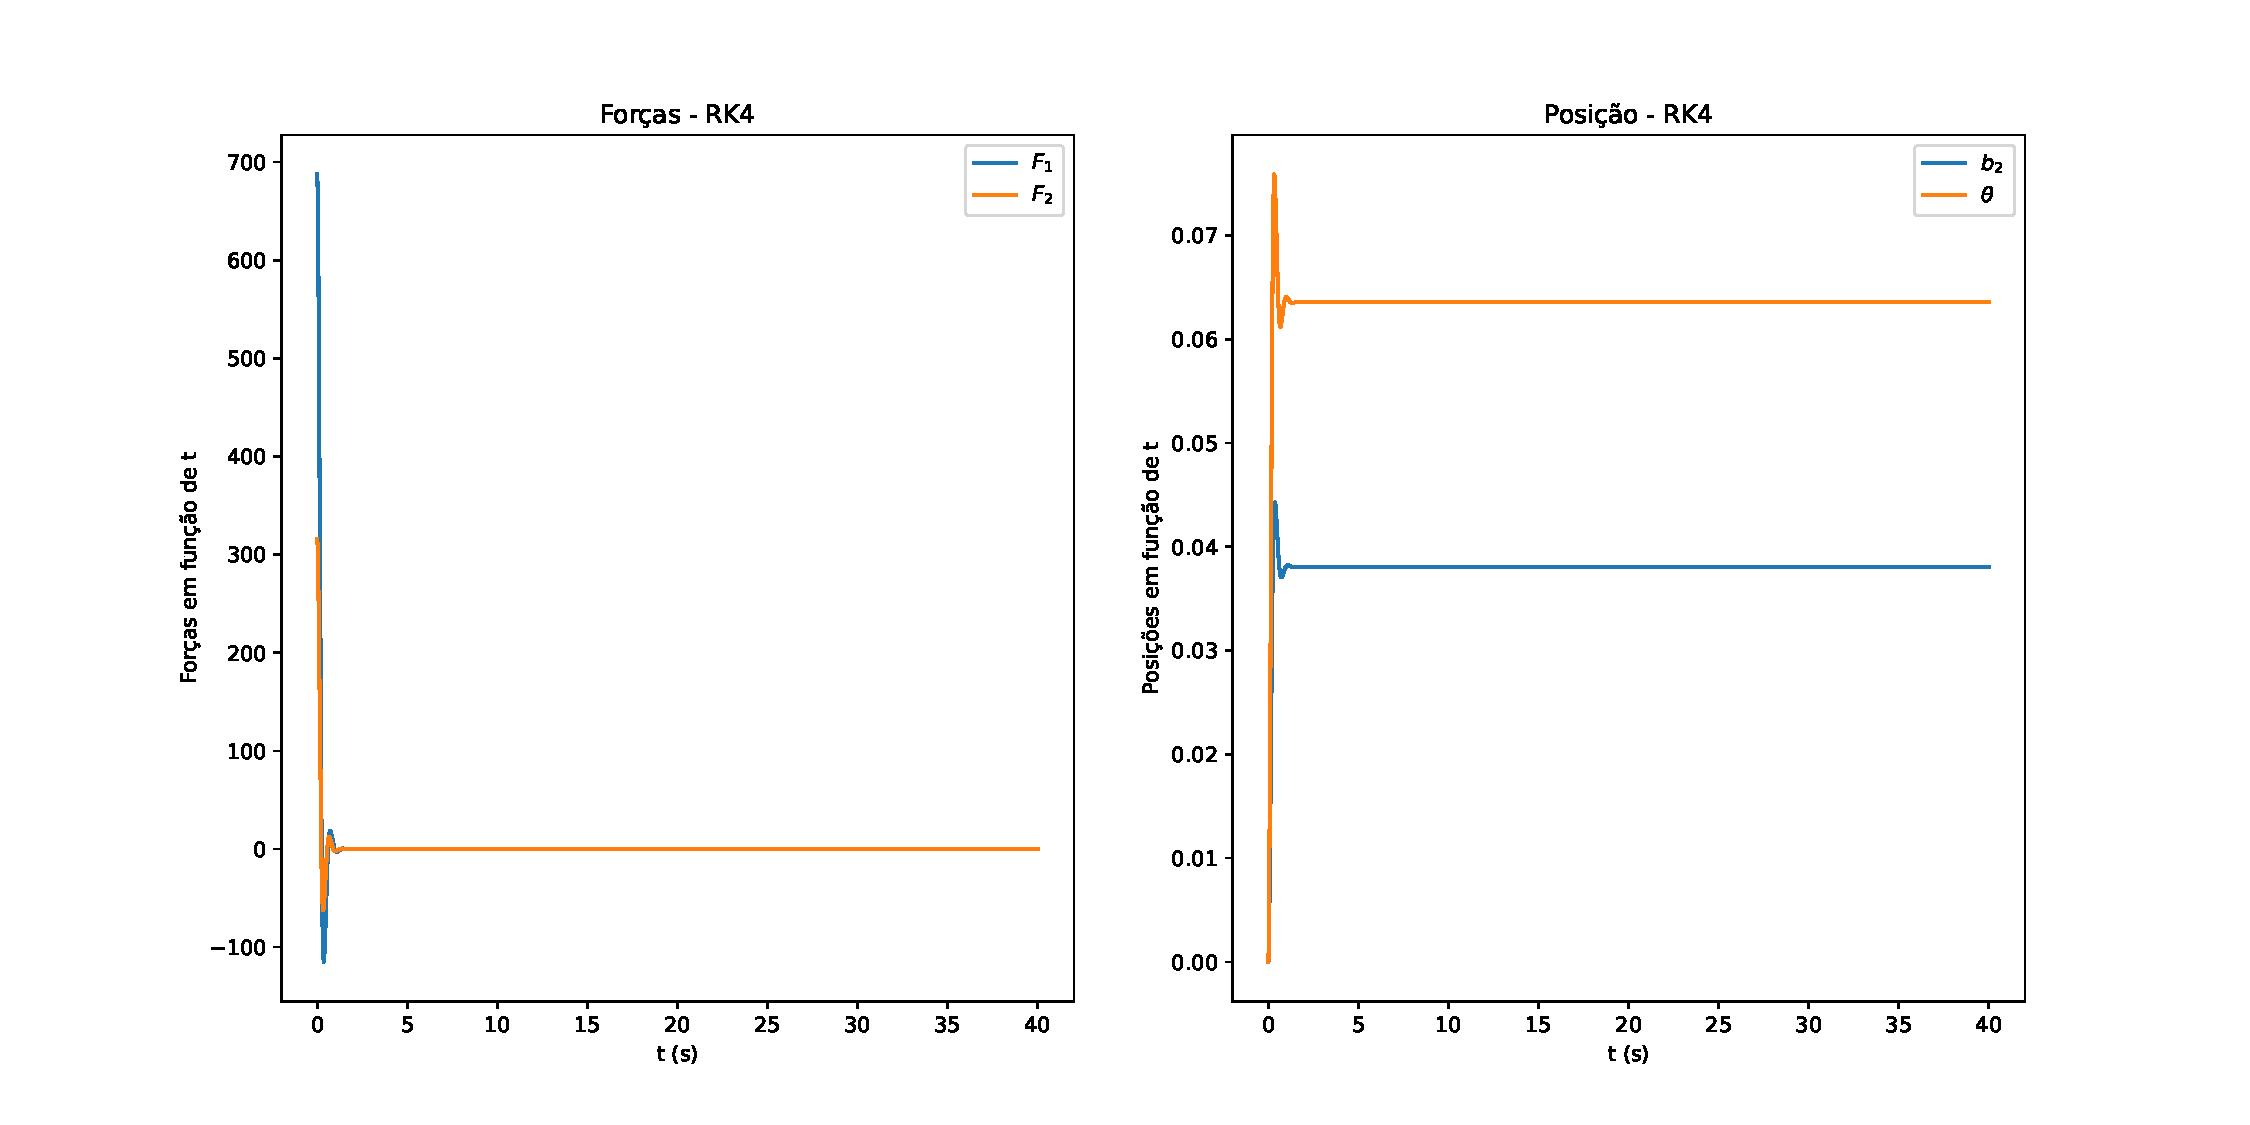
\includegraphics[width=\textwidth]{titanic/PVI_h=0.03_g1=4000.0_g2=10.0.pdf}
            \caption{$\gamma_2 = 10.0$}
        \end{subfigure}
        \caption{PVI com $\gamma_1 = 4000.0$ (Titanic)}
        \label{fig:titanic_PVI3}
    \end{figure}

    \begin{figure}[H]
        \centering
        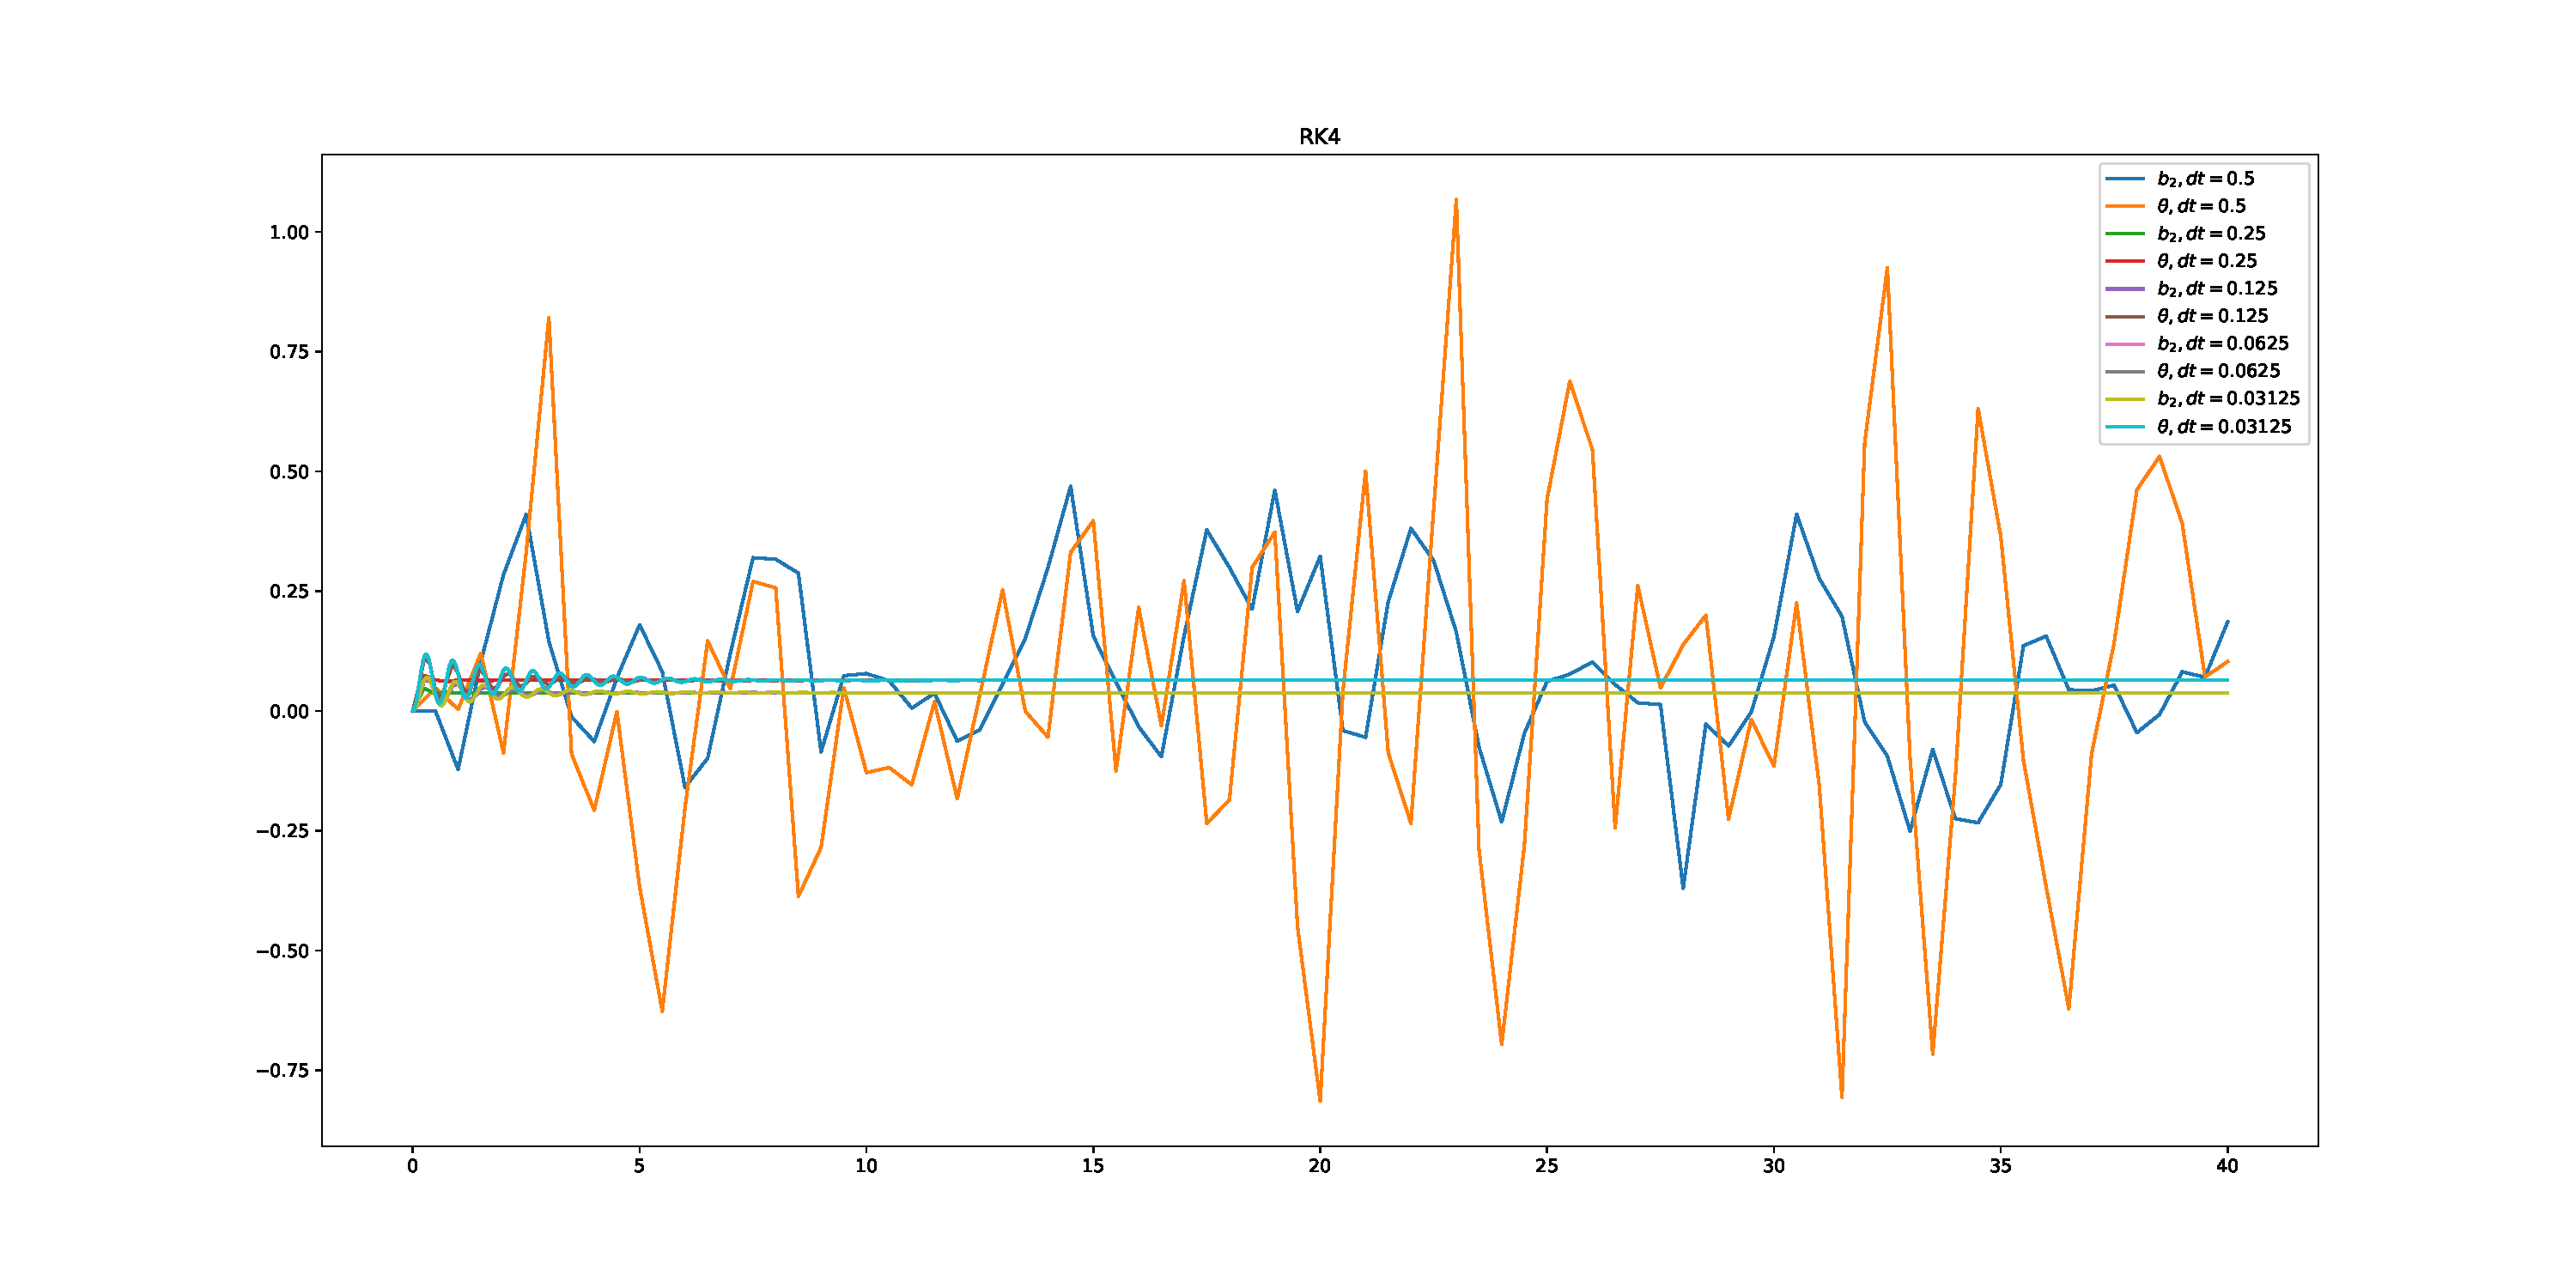
\includegraphics[width=\textwidth]{titanic/PVI_conv.pdf}
        \caption{$\theta$ e $b_2$ em função do tempo para diversos passos de tempo no caso do iceberg}
        \label{fig:titanic_conv1}
    \end{figure}

    \begin{figure}[H]
        \centering
        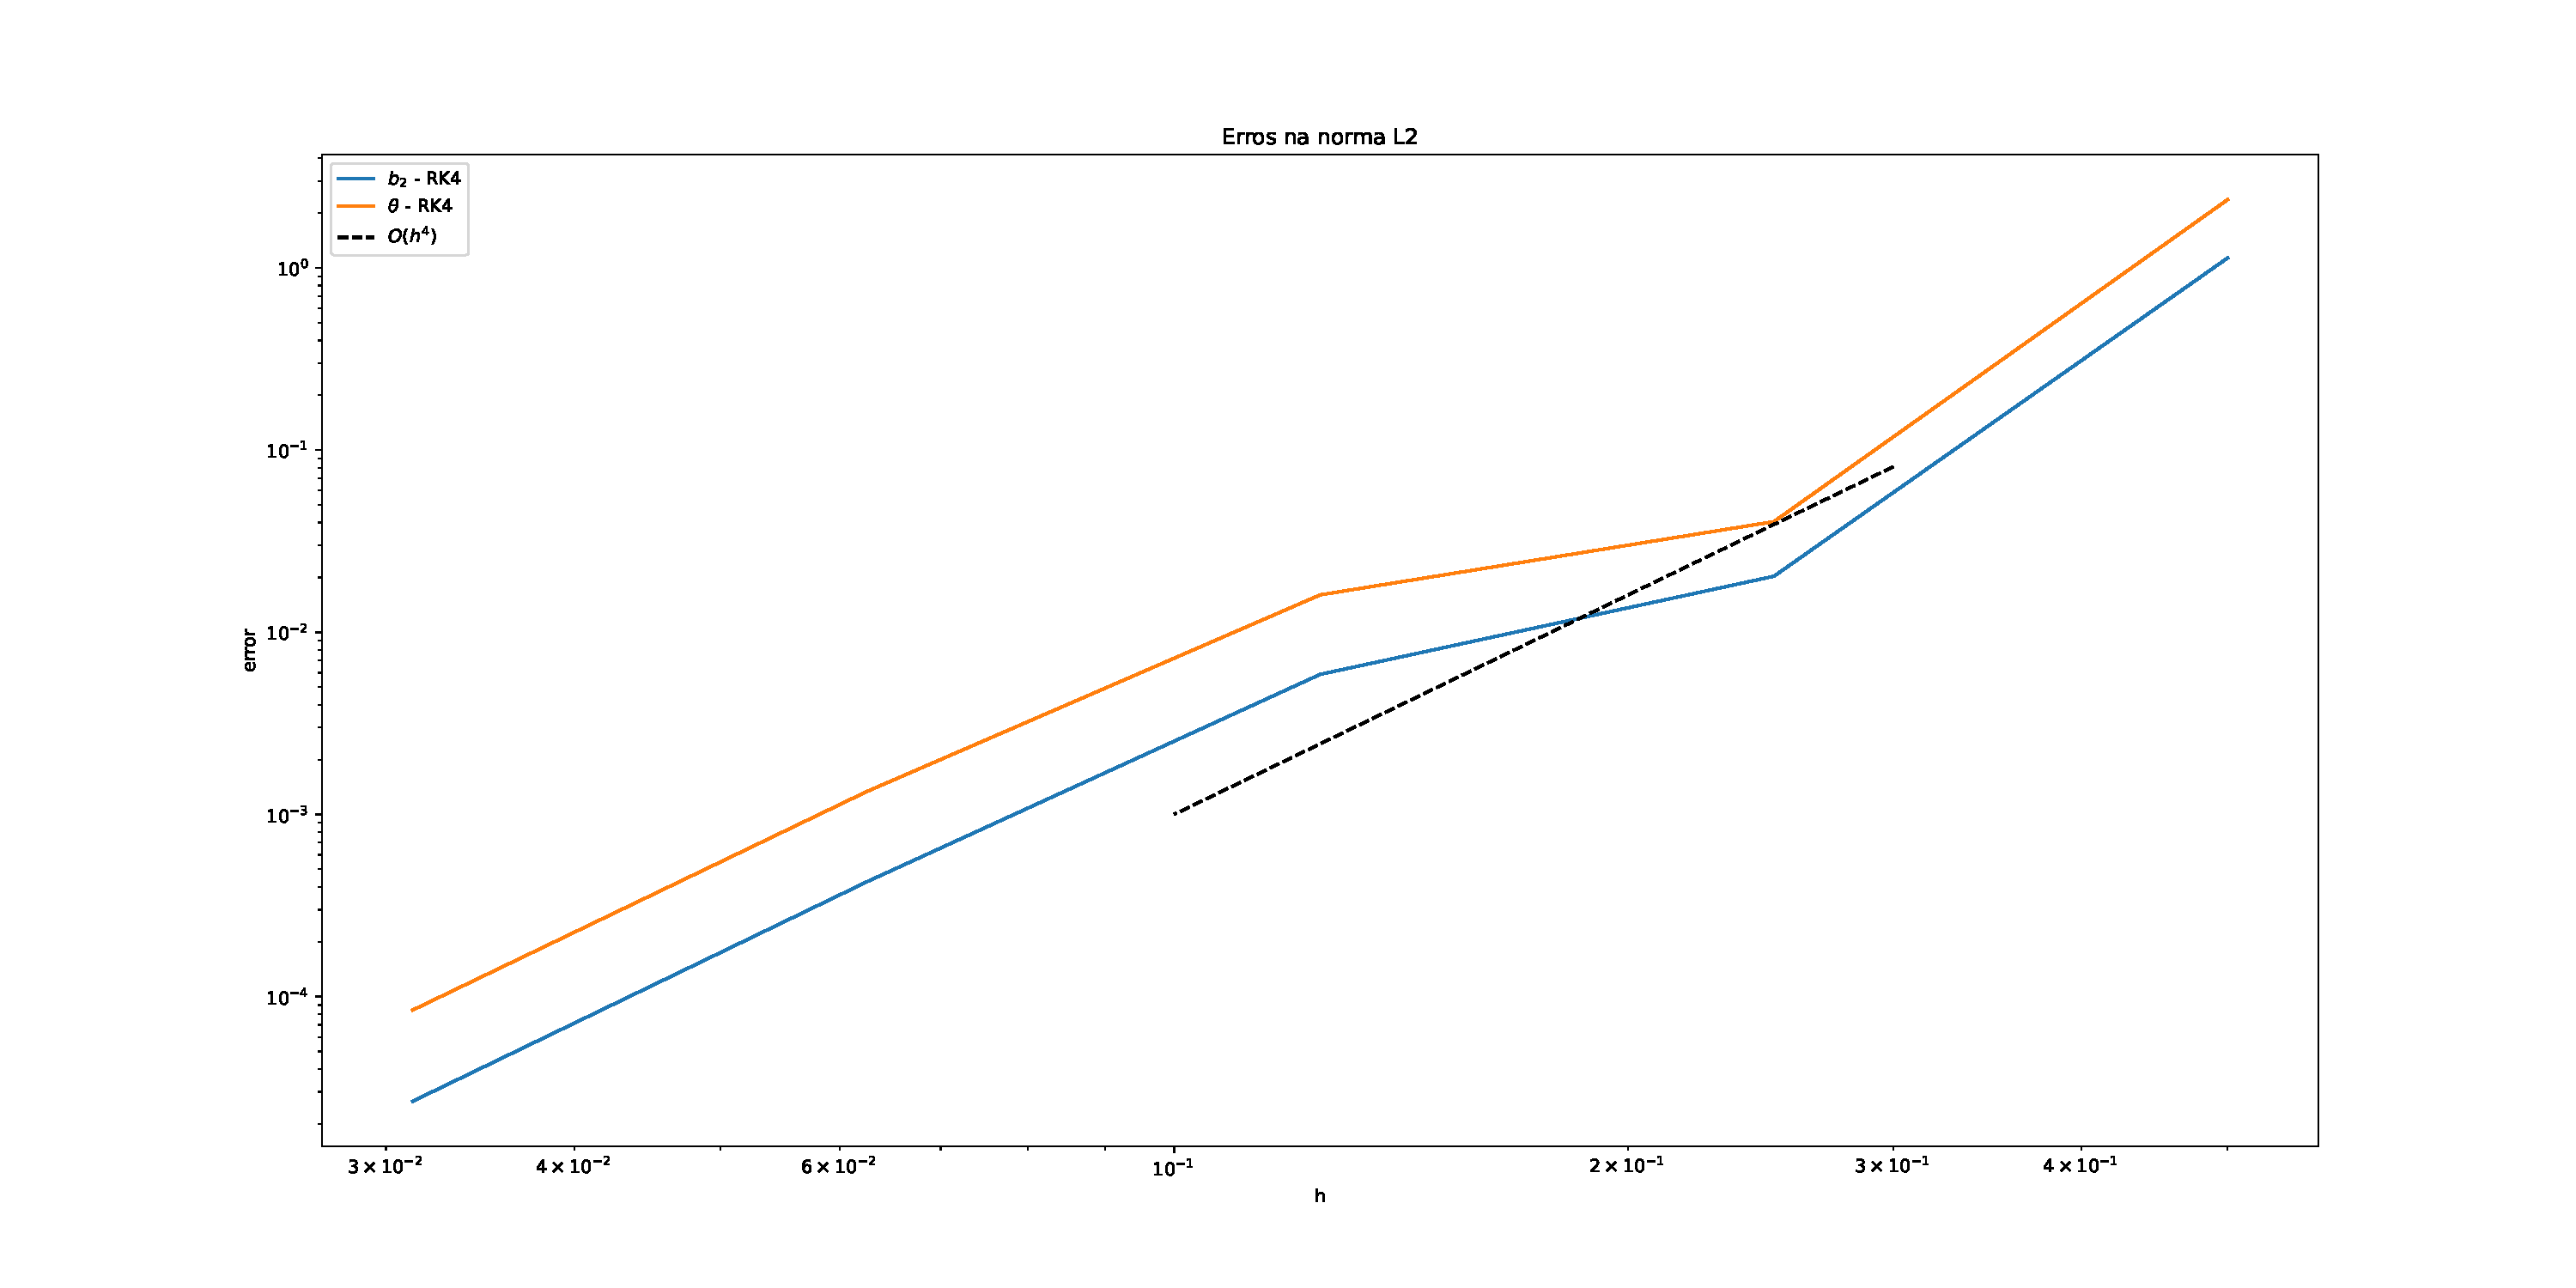
\includegraphics[width=\textwidth]{titanic/PVI_conv2.pdf}
        \caption{Ordem de convergência do método para solução do PVI (iceberg)}
        \label{fig:titanic_conv2}
    \end{figure}

    \FloatBarrier



    \subsection{Triângulo retângulo}
    \label{sec:triang}

    \subsubsection{Mapeamento de forças}
    A figura \ref{fig:triang_level} mostra o mapa de forças.
    \begin{figure}[H]
        \centering
        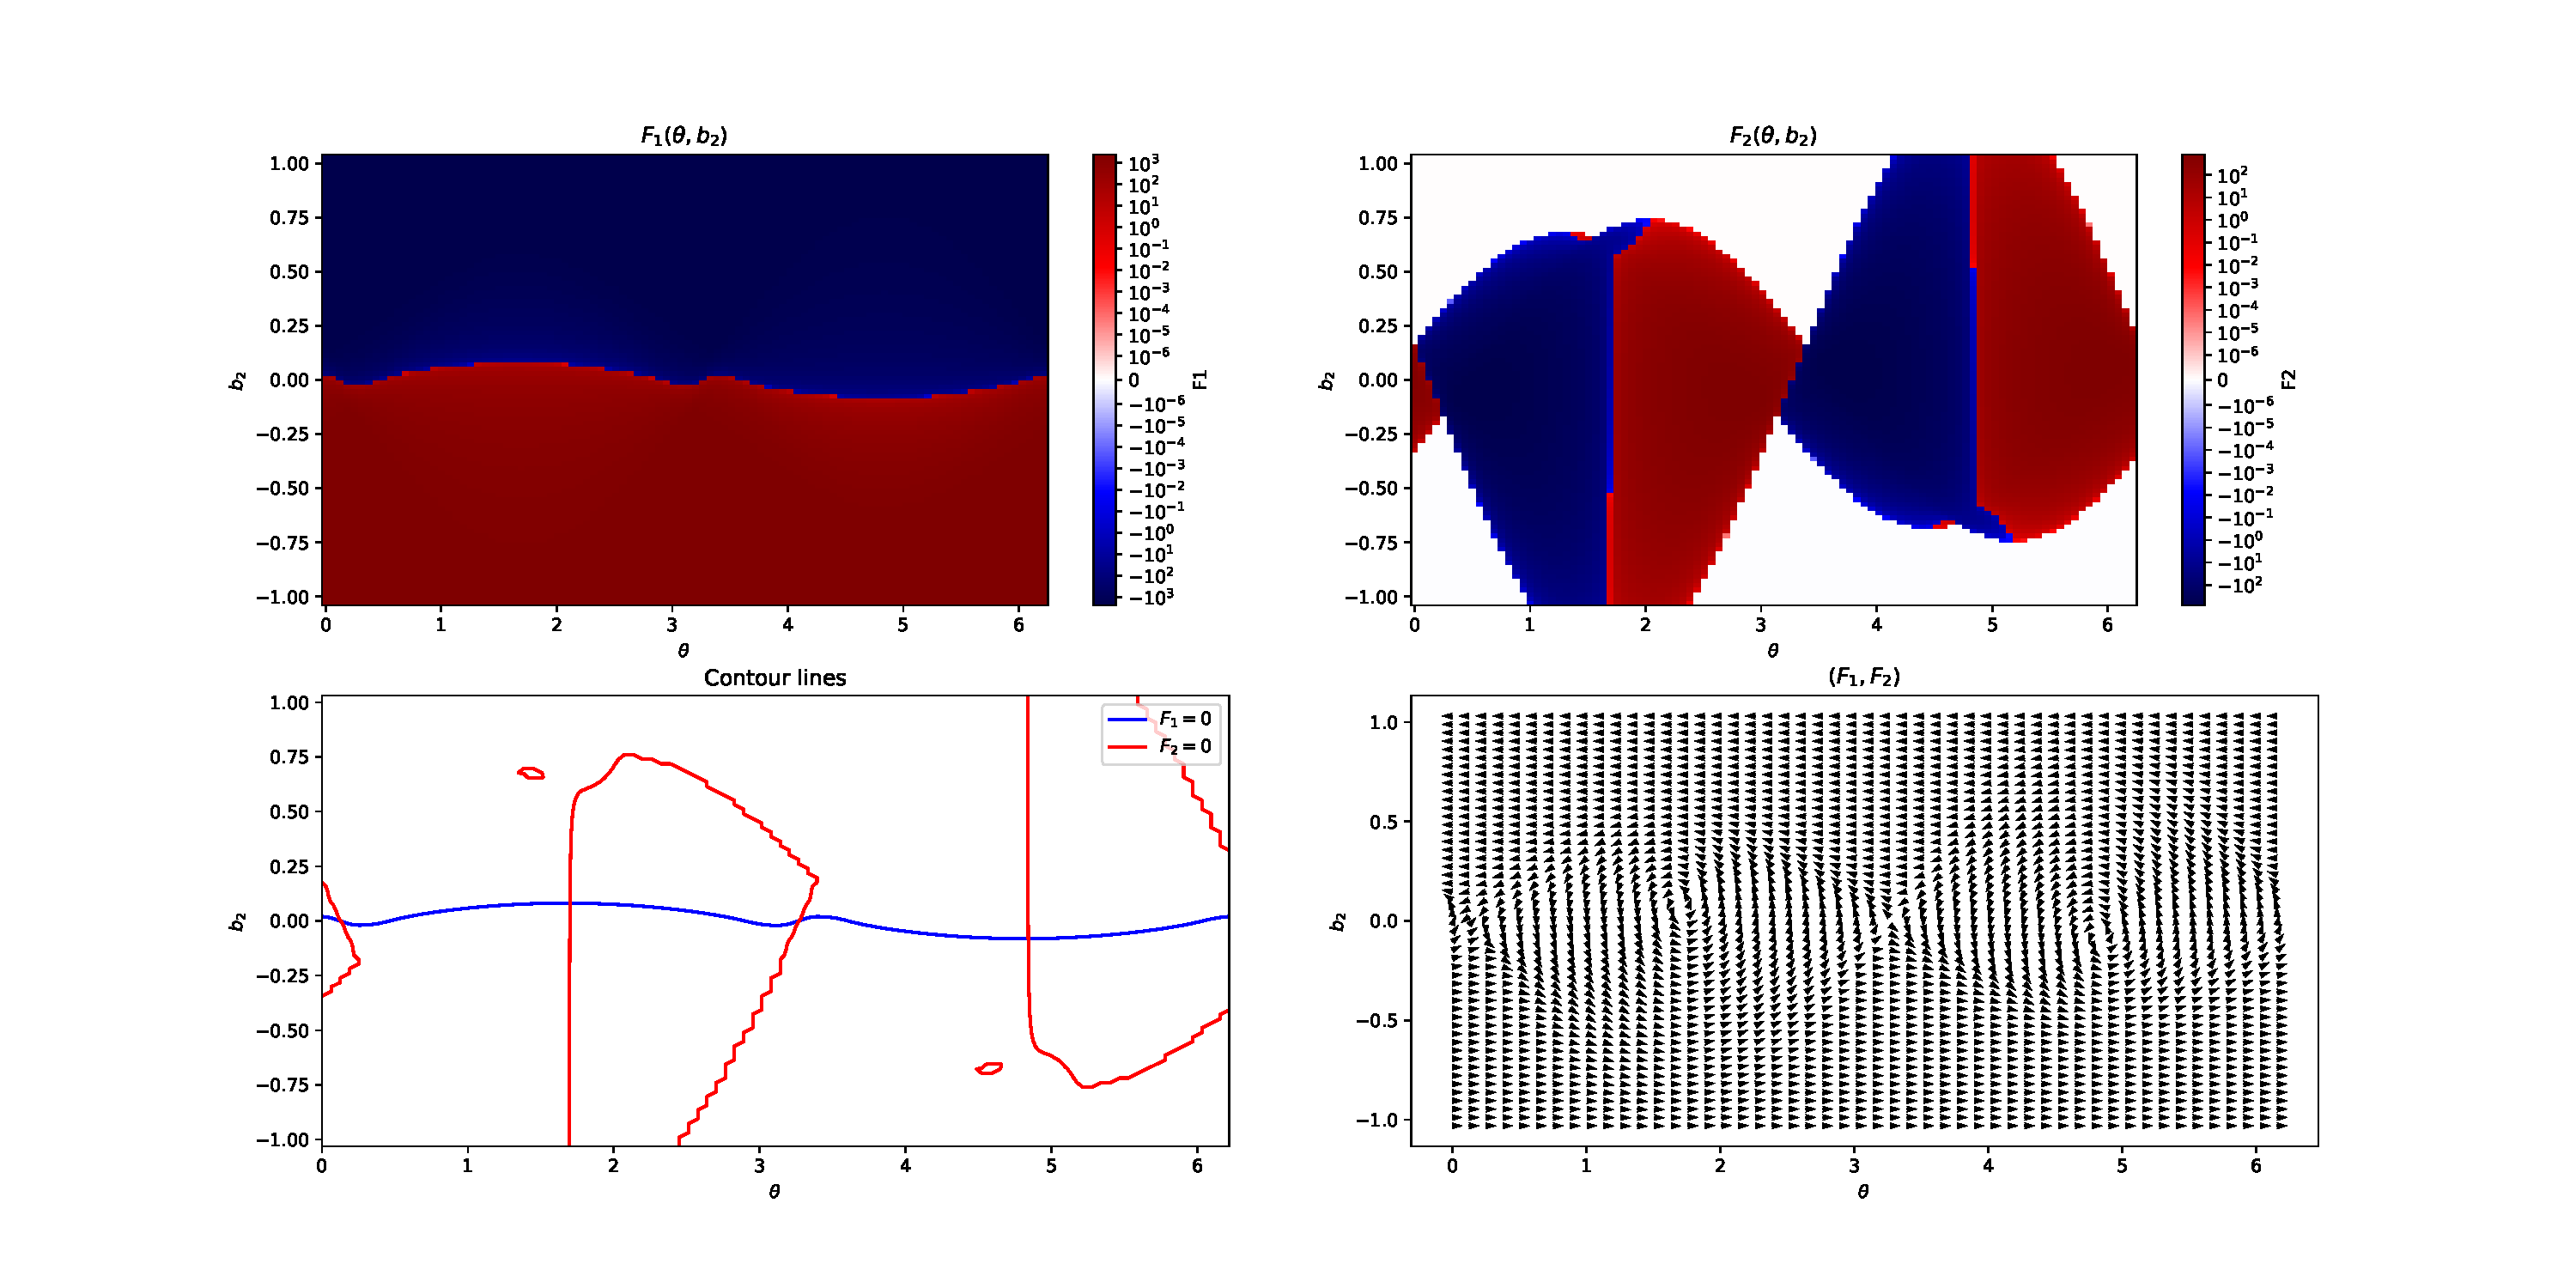
\includegraphics[width=\textwidth]{triangulo_retangulo/levels.pdf}
        \caption{Curvas de forças do triângulo retângulo}
        \label{fig:triang_level}
    \end{figure}
    
    Novamente, temos 4 pontos de equilíbrio, cuja aproximações sã dadas na tabela \ref{table:triang_approx}

    \begin{table}[H]
        \centering
        \begin{tabular}{ccc} \\

            
            \hline
            Índice do ponto & $\theta$ aproximado & $b_2$ aproximado \\

            \hline
            1 & 0.00 & 0.10 \\
            2 & 1.80 & 0.00 \\
            3 & 3.20 & 0.00 \\
            4 & $3\pi/2$ & 0.00 \\

            \hline
        \end{tabular}
        \caption{Aproximações dos pontos de equilíbrio do triângulo retângulo}
        \label{table:triang_approx}
    \end{table}
    
    O formato do campo de forças é análogo ao campo do Titanic, logo, os pontos 2 e 4 são pontos de equilíbrio instável, enquanto sobre os pontos 1 e 3 não é possível concluir nada.

    \subsubsection{Pontos de equilíbrio}
    Os pontos de equilíbrio estão visualmente representados na figura \ref{fig:triang_equi}, enquanto suas coordenadas estão na tabela \ref{table:triang_approx}.
    \begin{figure}[H]
        \centering
        \begin{subfigure}[b]{0.4\textwidth}
            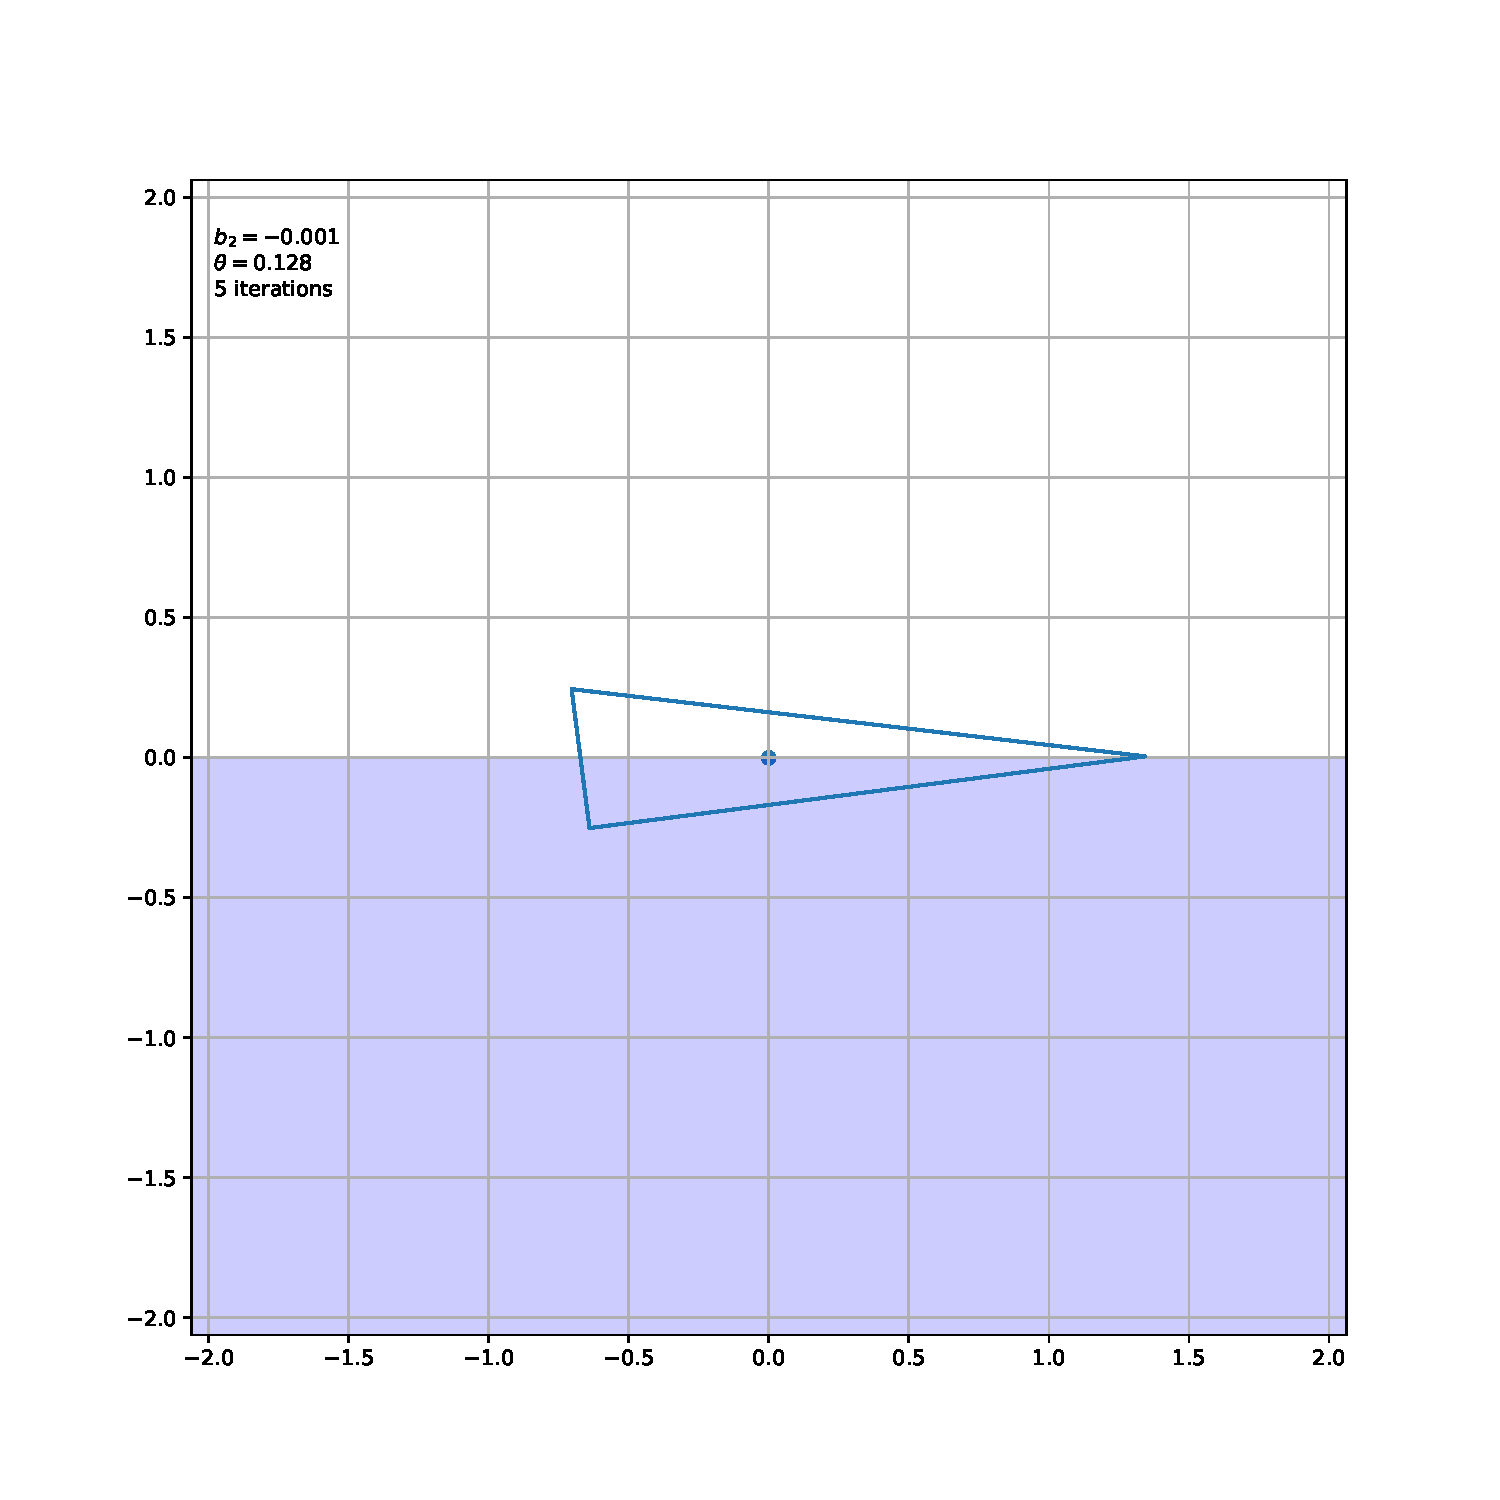
\includegraphics[width=\textwidth]{triangulo_retangulo/newton_b0=0.100_theta0=0.000.pdf}
            \caption{Partindo do ponto 1}    
        \end{subfigure}
        \quad
        \begin{subfigure}[b]{0.4\textwidth}
            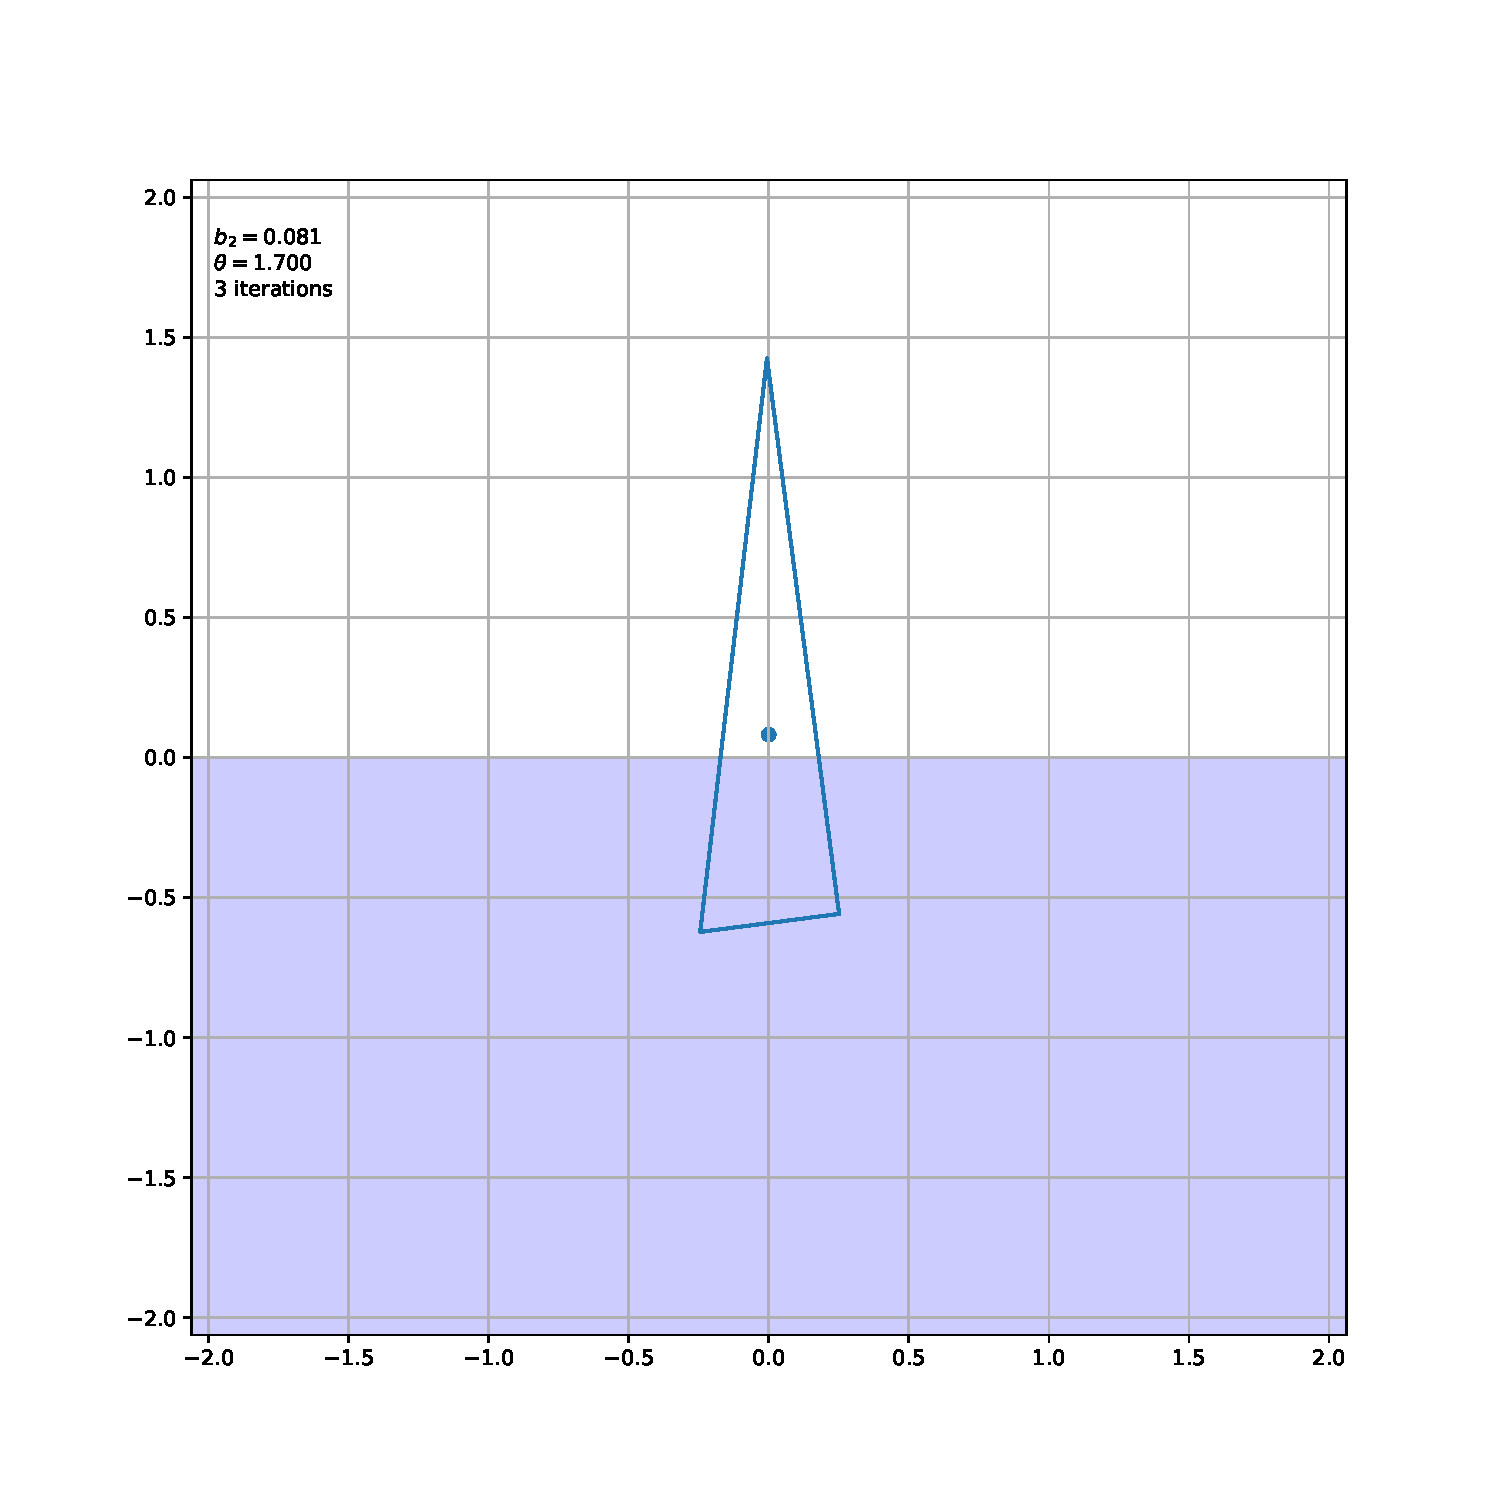
\includegraphics[width=\textwidth]{triangulo_retangulo/newton_b0=0.000_theta0=1.800.pdf}   
            \caption{Partindo do ponto 2}
        \end{subfigure}
        \quad
        \begin{subfigure}[b]{0.4\textwidth}
            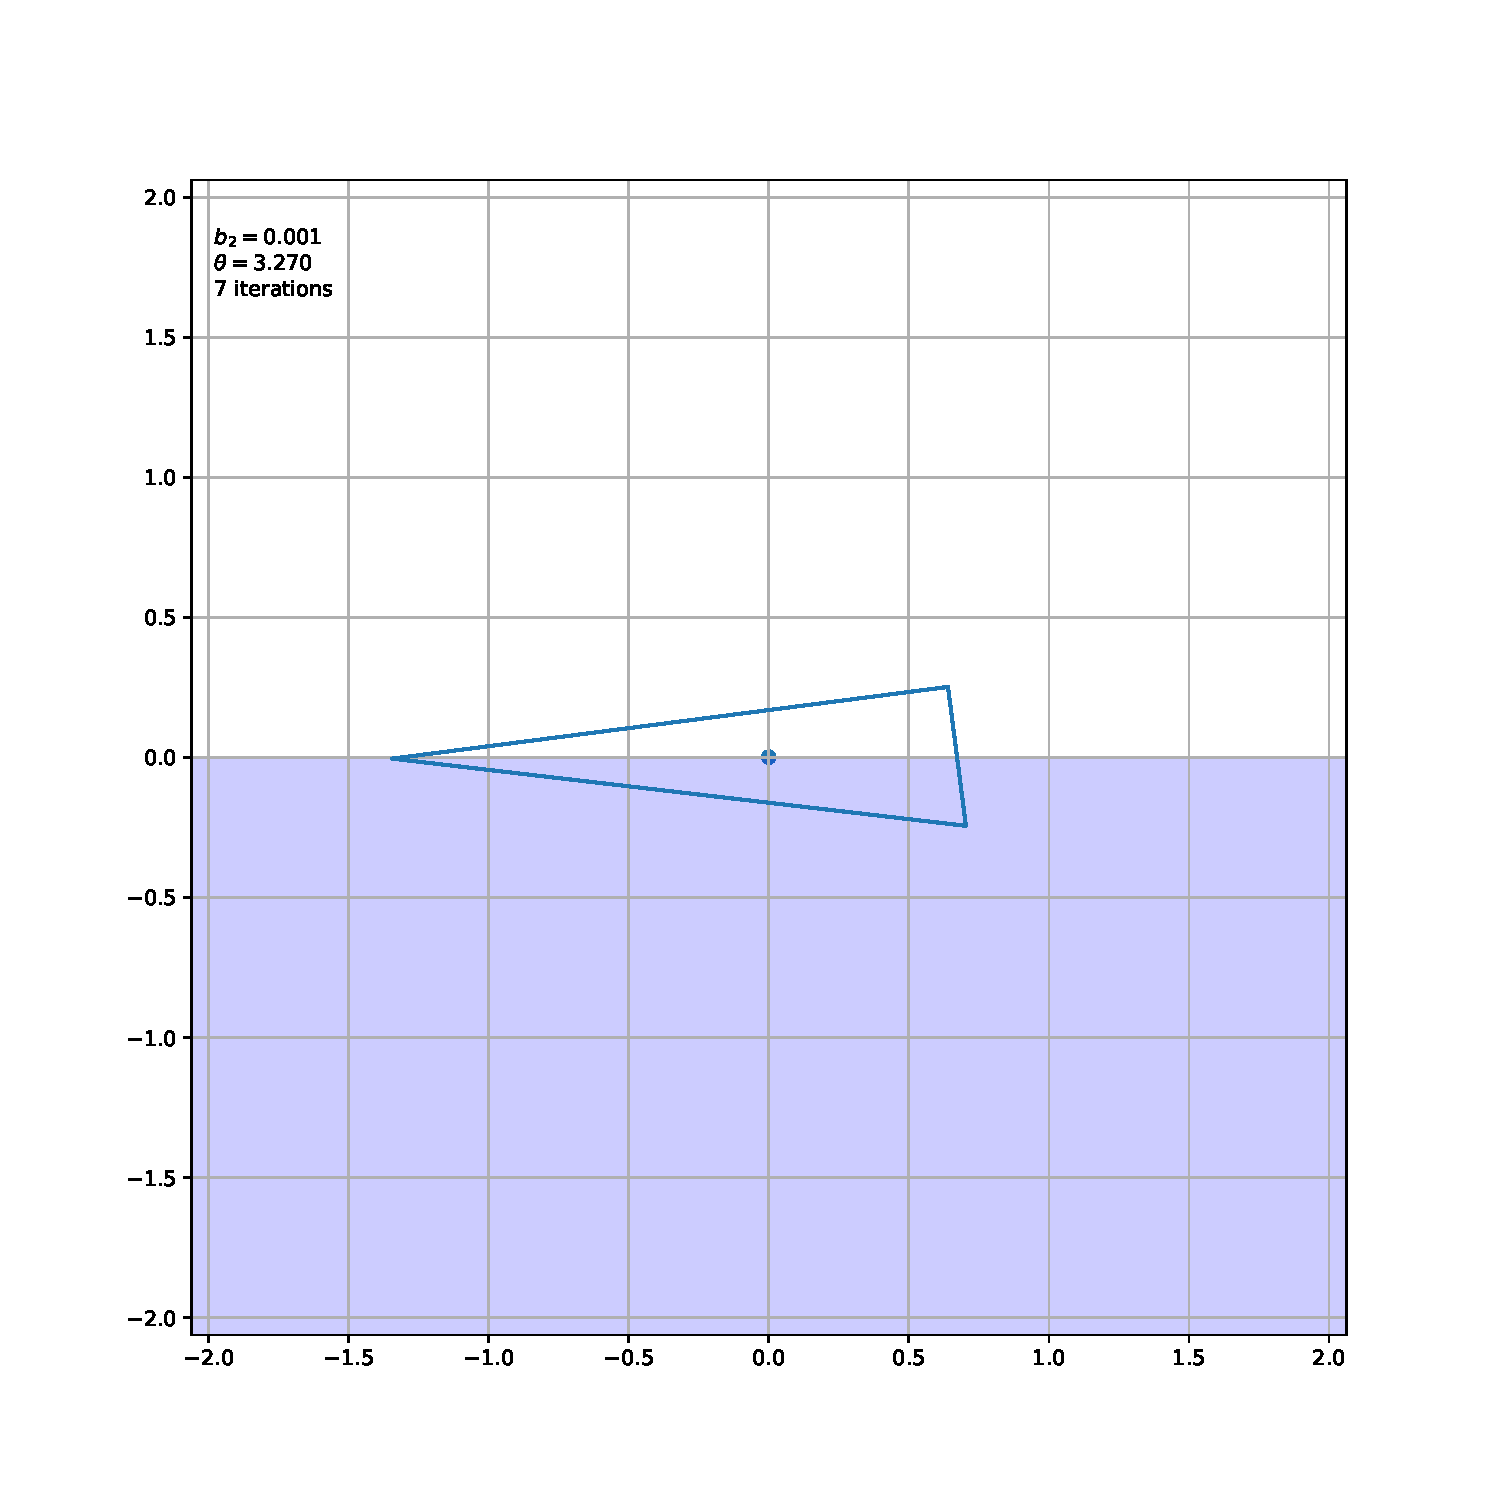
\includegraphics[width=\textwidth]{triangulo_retangulo/newton_b0=0.000_theta0=3.200.pdf}
            \caption{Partindo do ponto 3}    
        \end{subfigure}
        \quad
        \begin{subfigure}[b]{0.4\textwidth}
            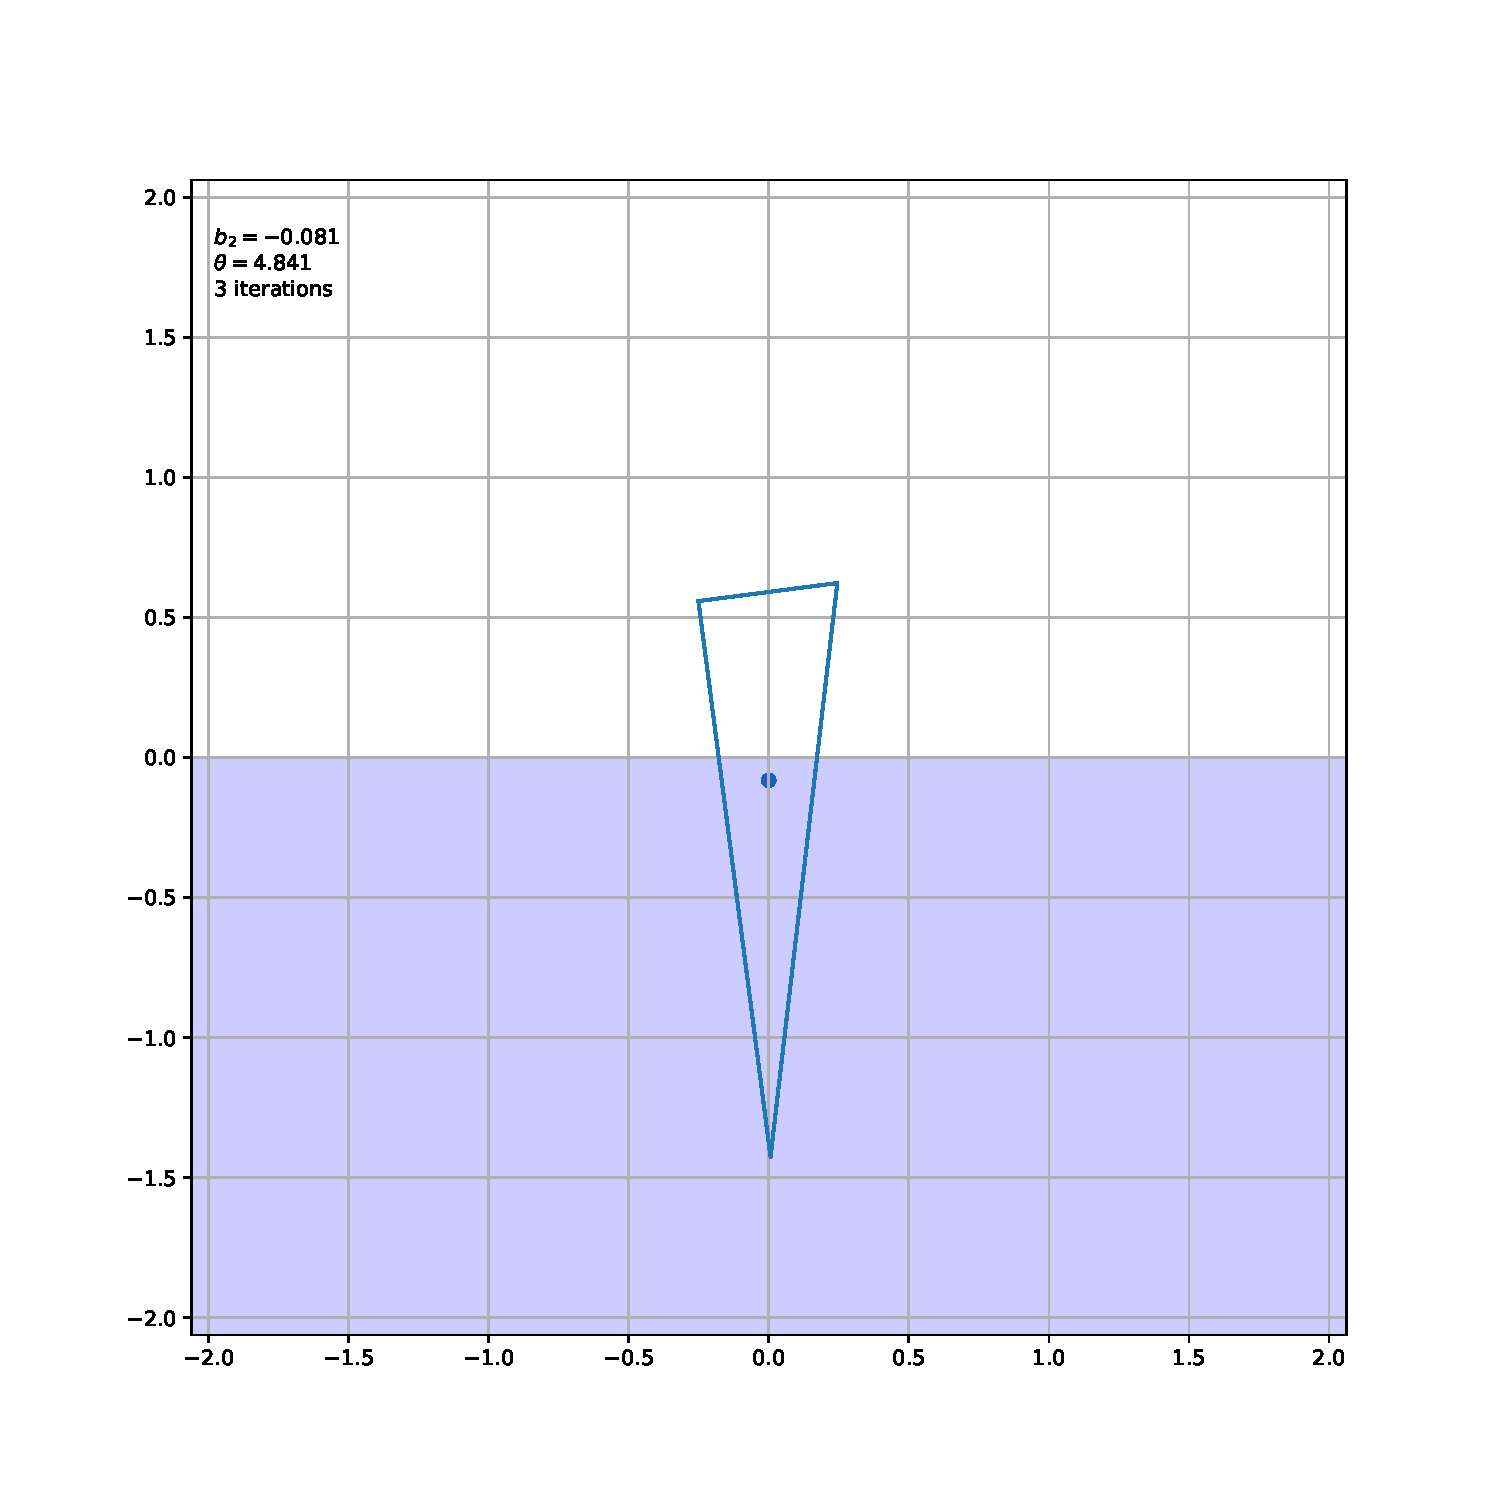
\includegraphics[width=\textwidth]{triangulo_retangulo/newton_b0=0.000_theta0=4.712.pdf}
            \caption{Partindo do ponto 4}    
        \end{subfigure}
        \quad
        
        \caption{Pontos de equilíbrio encontrados para o triângulo retângulo}
        \label{fig:triang_equi}
    \end{figure}
    
    \begin{table}[H]
        \centering
        \begin{tabular}{ccccc} \\

            
            \hline
            Índice & $\theta$ & $b_2$ & Iterações & Ordem média de convergência \\

            \hline
            1 & 0.128 & -0.001  & 5 & 1.514\\
            2 & 1.700 & 0.081 & 3 & 1.795\\
            3 & 3.270 & 0.001 & 7 & 1.811\\
            4 & 4.841 & -0.081 & 3 & 1.602 \\

            \hline
        \end{tabular}
        \caption{Pontos de equilíbrio encontrados para o triângulo retângulo}
        \label{table:triang_equi}
    \end{table}
    
    A ordem de convergência do método de Newton foi derrubada em todos os casos. Inclusive, para esse objeto, encontrar aproximações boas o suficiente para o método de Newton convergir para uma solução específica foi um processo um tanto quanto mais complicado do que para os outros objetos. Uma possível causa para isso será dada na seção \ref{sec:geo}.
    

    \subsubsection{Análise dinâmica}

    Os resultados das soluções dos PVIs para o triângulo são semelhantes à solução do Titanic. Apesar disso, pode-se ver que as oscilações das coordenadas do corpo são, de certa forma, mais irregulares. Novamente é evidenciado o forte acoplamento entre $\theta$ e $b_2$ pelas Figuras \ref{fig:triang_PVI1}, \ref{fig:triang_PVI2} e \ref{fig:triang_PVI1}. Para todos os casos que entraram em estado estacionário, o ponto de equilíbrio encontrado foi o ponto 1.

    A ordem de convergência do RK4 para o triângulo retângulo se aproxima da teórica, exceto para alguns valores de $h$ (figura \ref{fig:triang_conv2}). Devido à natureza oscilatória "suja" do objeto, passos de tempo com ordem de grandeza maiores que $1e-2$ são inutilizáveis, como pode ser visto na figura \ref{fig:triang_conv1}.
    \begin{figure}
        \centering
        \begin{subfigure}[b]{0.9\textwidth}
            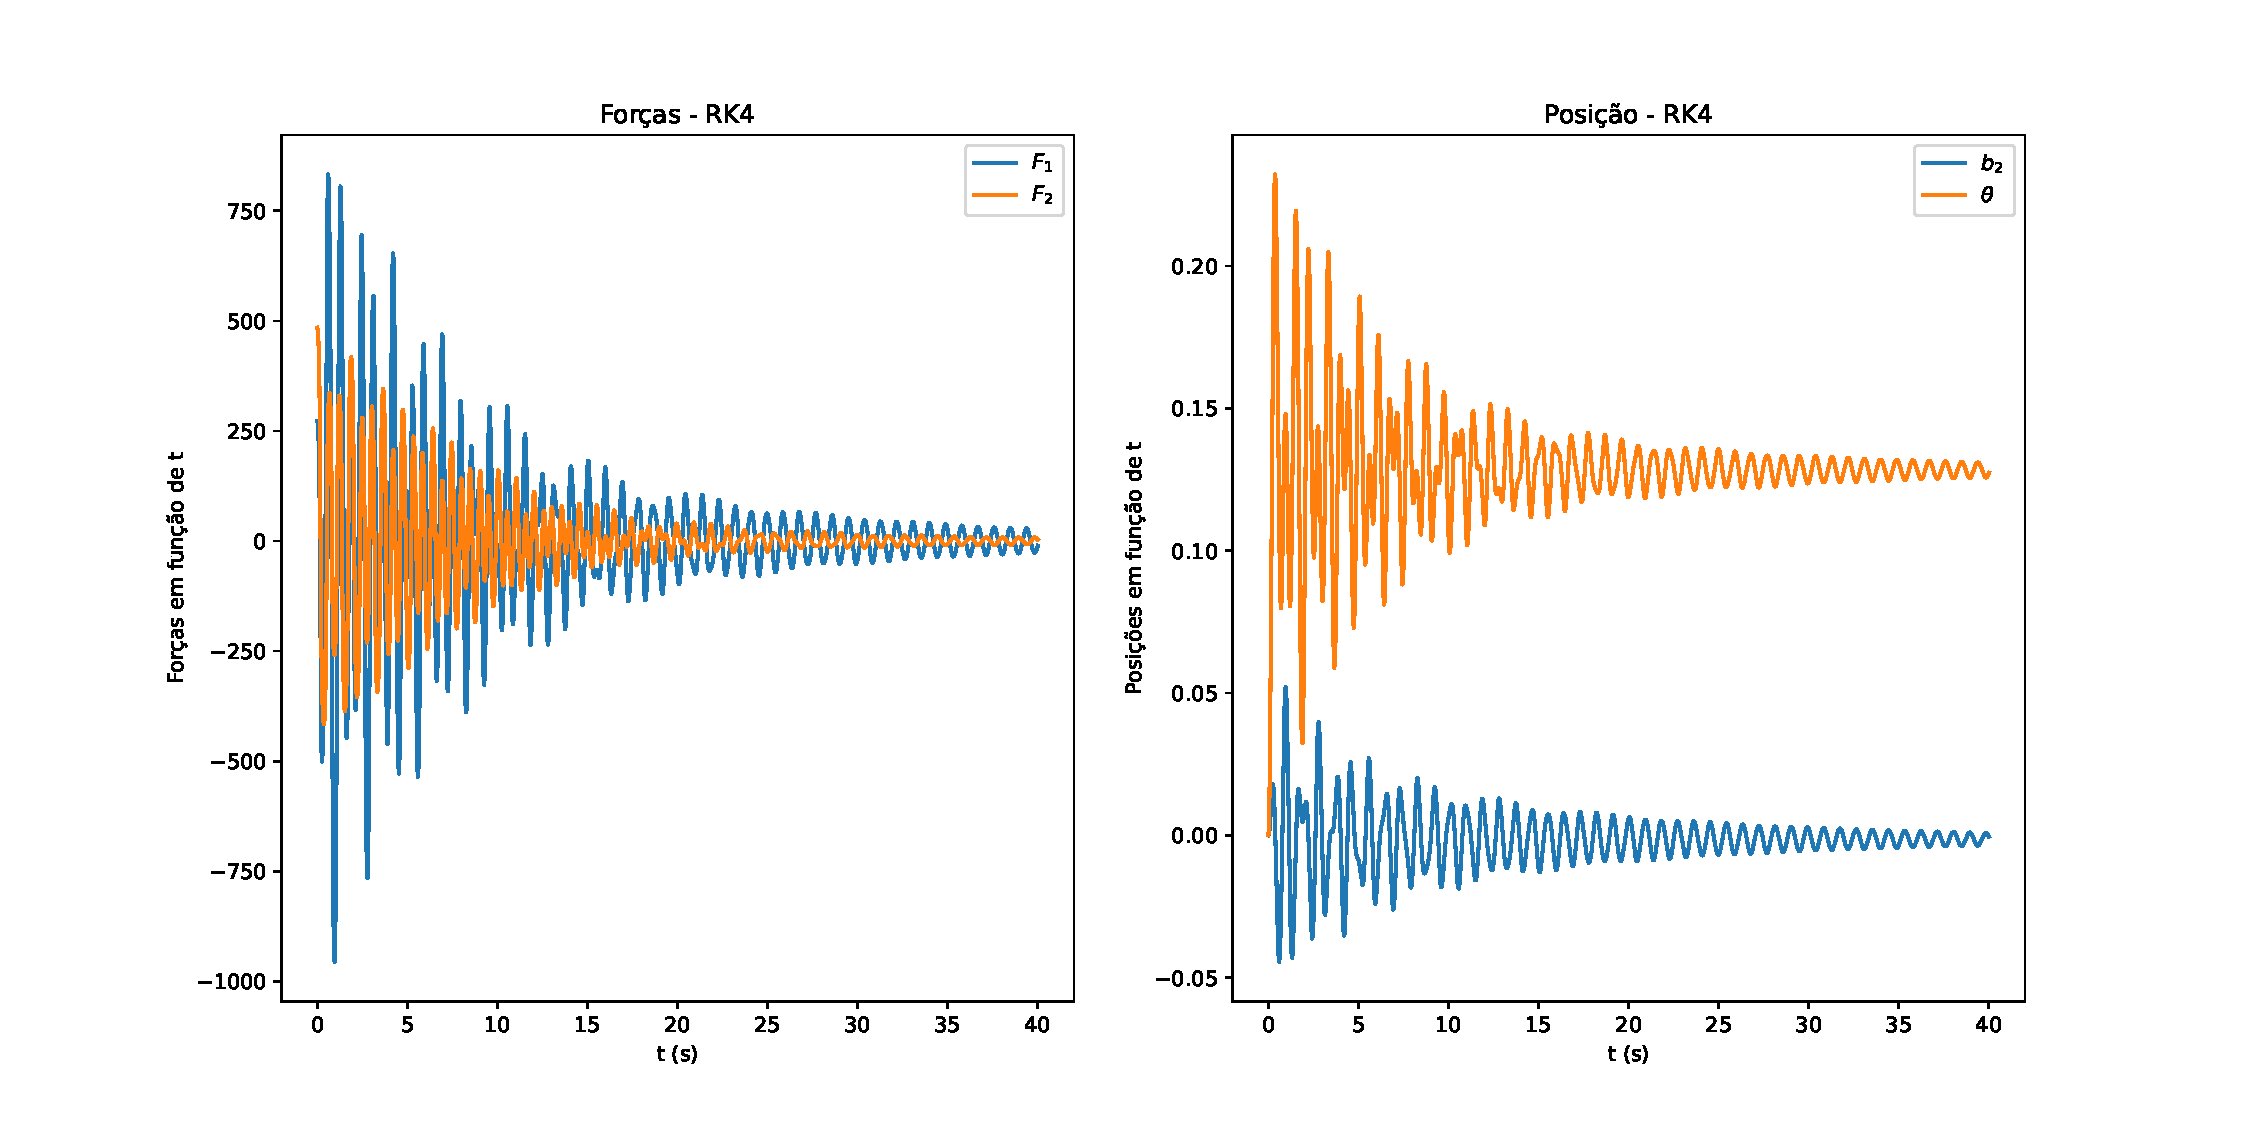
\includegraphics[width=\textwidth]{triangulo_retangulo/PVI_h=0.03_g1=1.0_g2=0.5.pdf}
            \caption{$\gamma_2 = 0.5$}
        \end{subfigure}
        \quad
        \begin{subfigure}[b]{0.9\textwidth}
            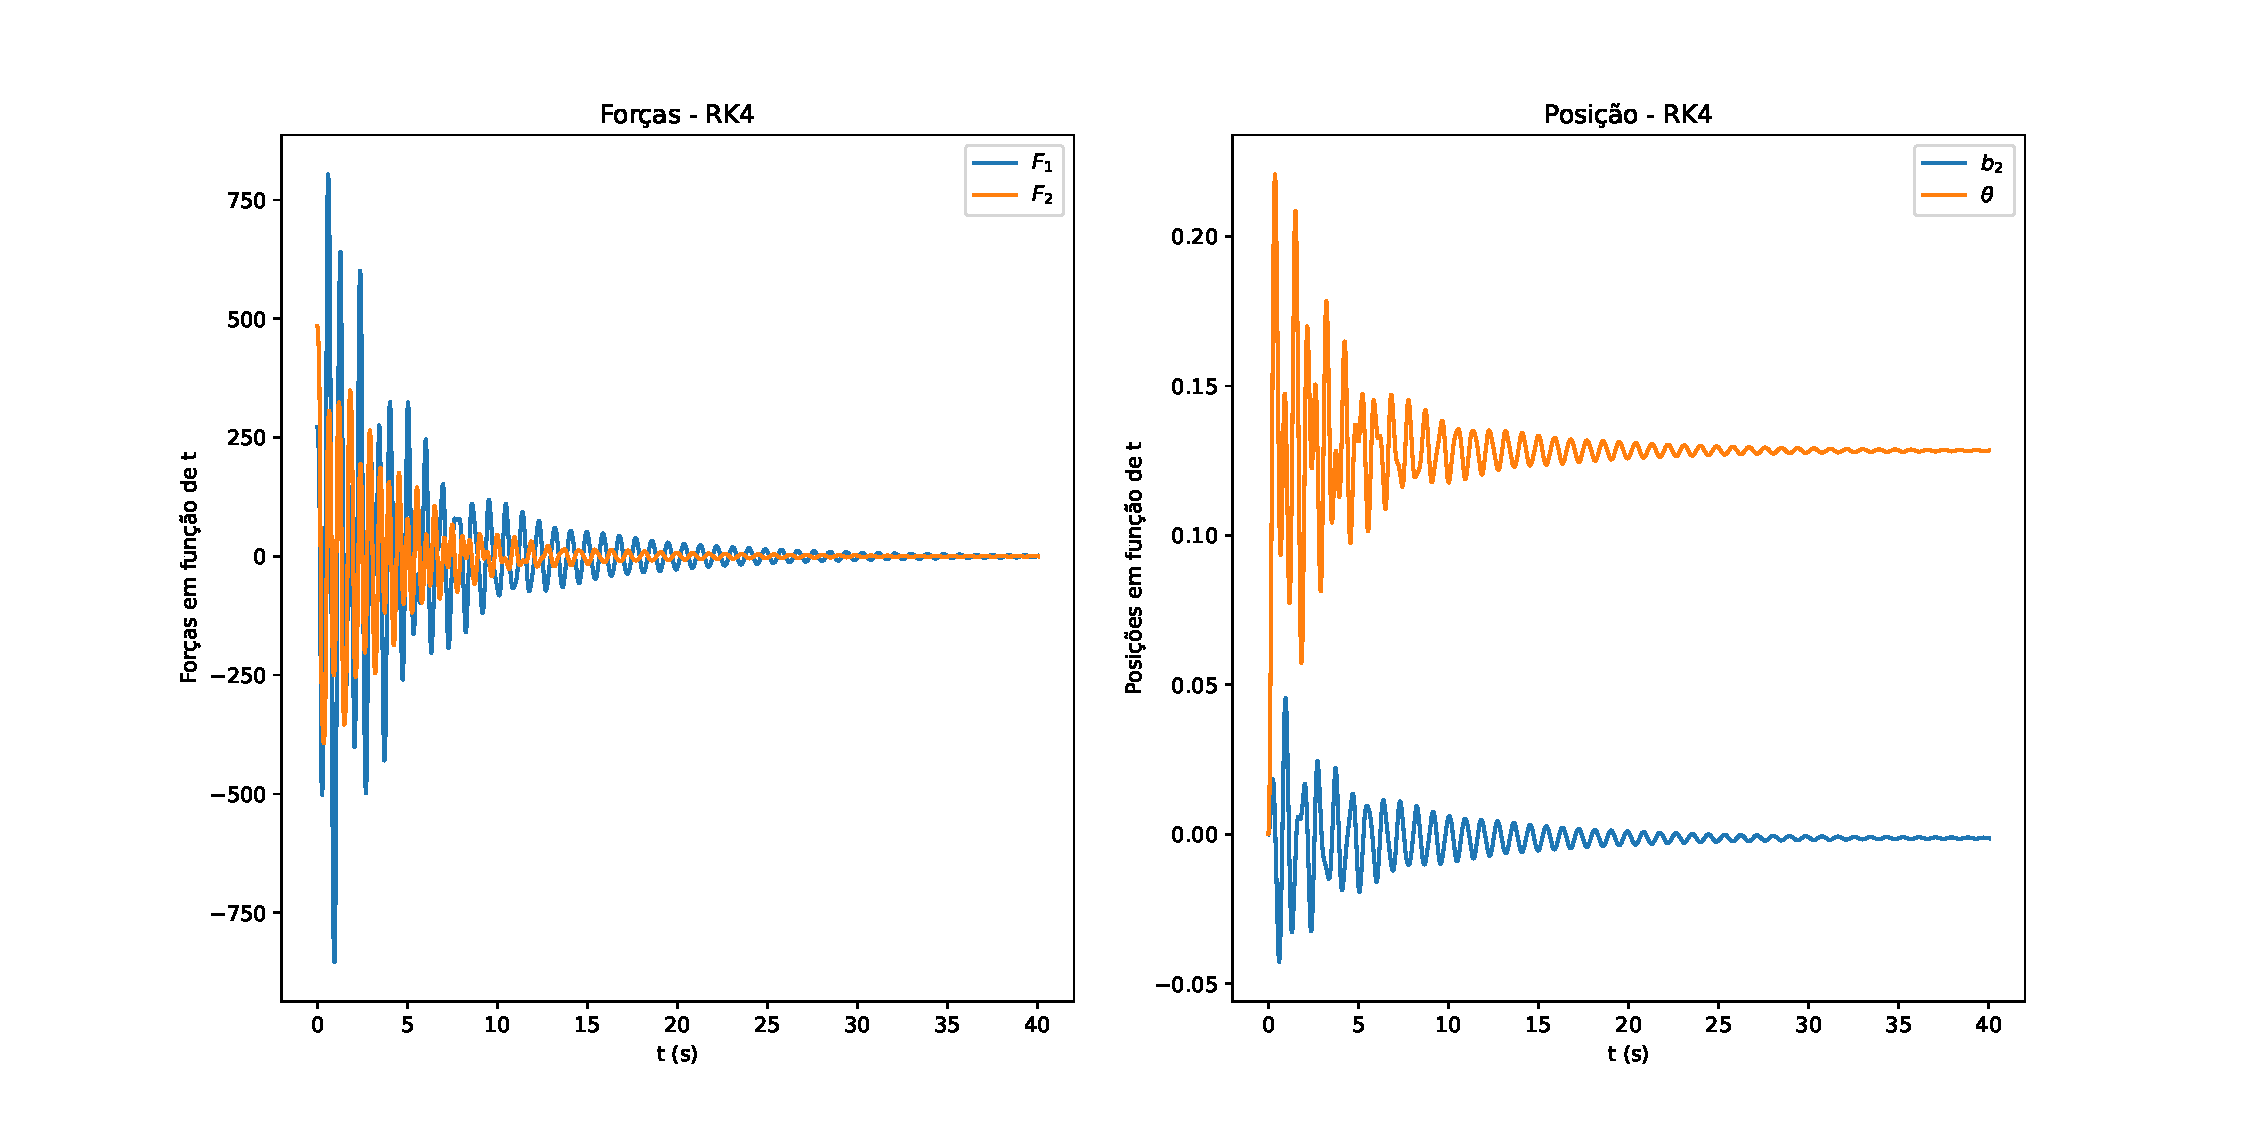
\includegraphics[width=\textwidth]{triangulo_retangulo/PVI_h=0.03_g1=1.0_g2=1.0.pdf}
            \caption{$\gamma_2 = 1.0$}
        \end{subfigure}
        \quad
        \begin{subfigure}[b]{0.9\textwidth}
            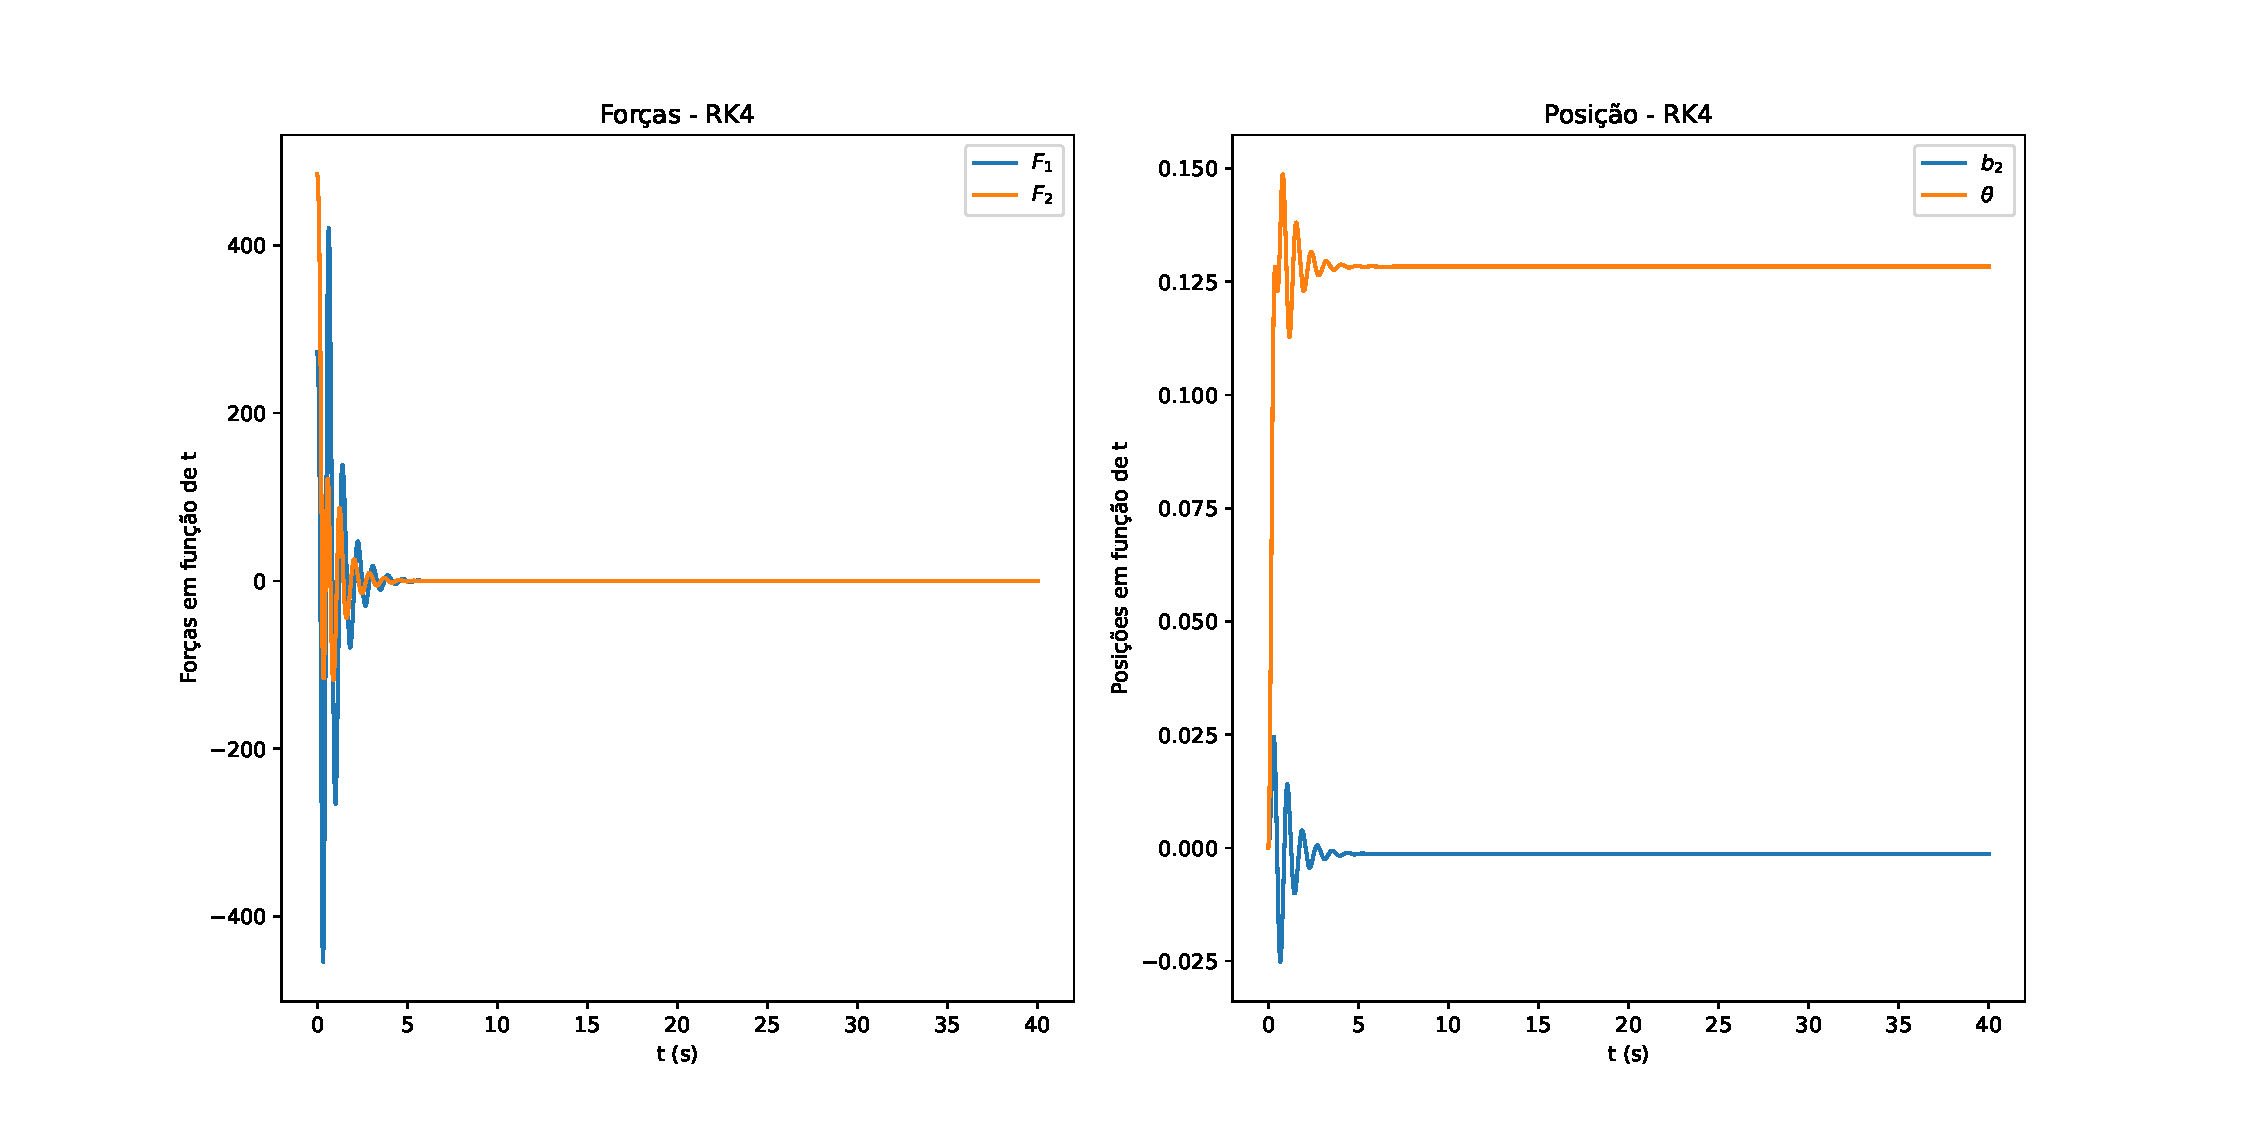
\includegraphics[width=\textwidth]{triangulo_retangulo/PVI_h=0.03_g1=1.0_g2=10.0.pdf}
            \caption{$\gamma_2 = 10.0$}
        \end{subfigure}
        \caption{PVI com $\gamma_1 = 1.0$ (Triângulo)}
        \label{fig:triang_PVI1}
    \end{figure}

    \begin{figure}
        \centering
        \begin{subfigure}[b]{0.9\textwidth}
            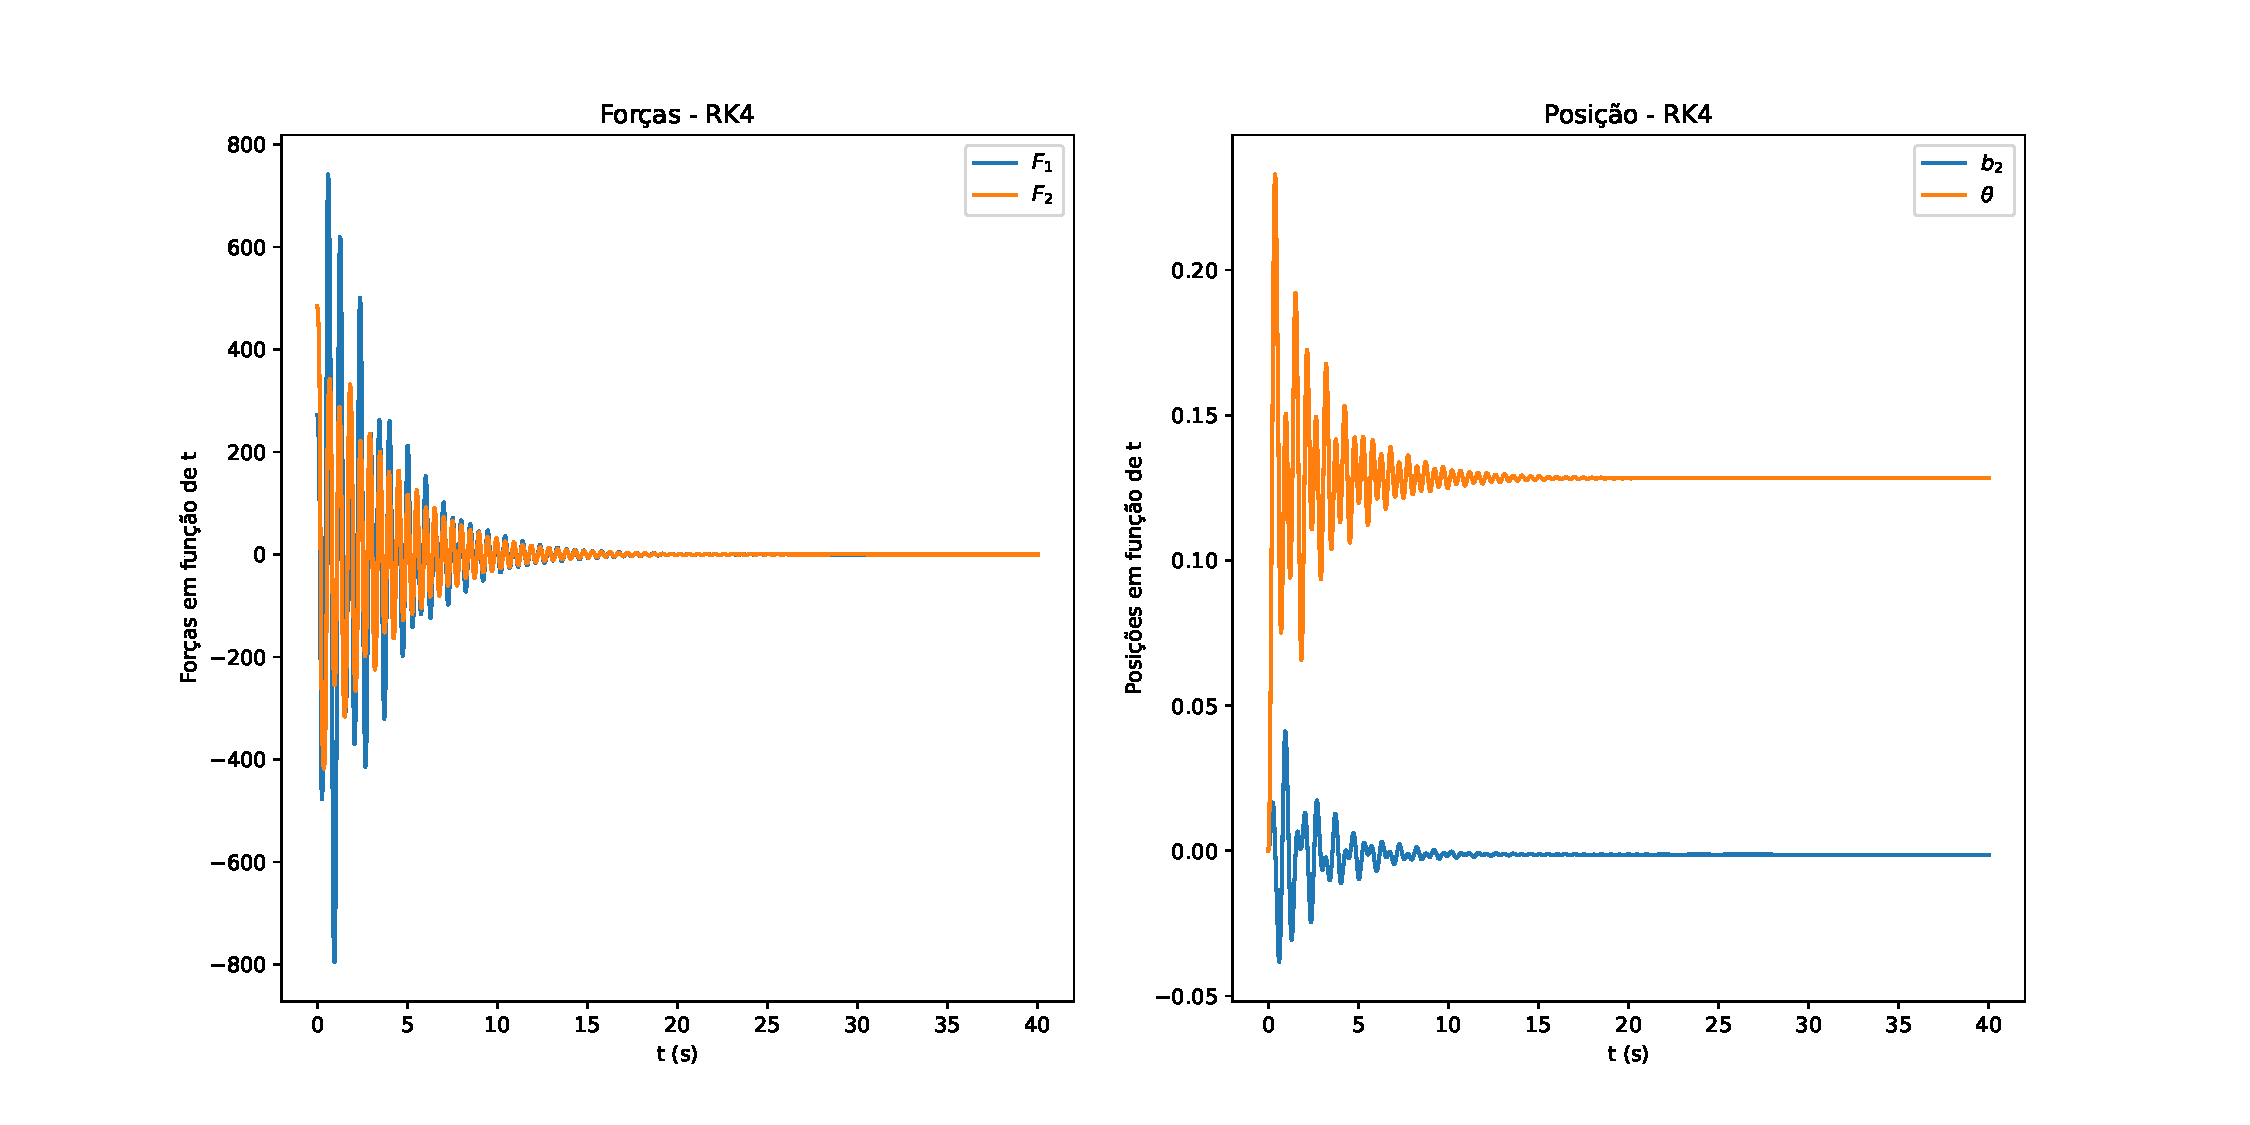
\includegraphics[width=\textwidth]{triangulo_retangulo/PVI_h=0.03_g1=500.0_g2=0.5.pdf}
            \caption{$\gamma_2 = 0.5$}
        \end{subfigure}
        \quad
        \begin{subfigure}[b]{0.9\textwidth}
            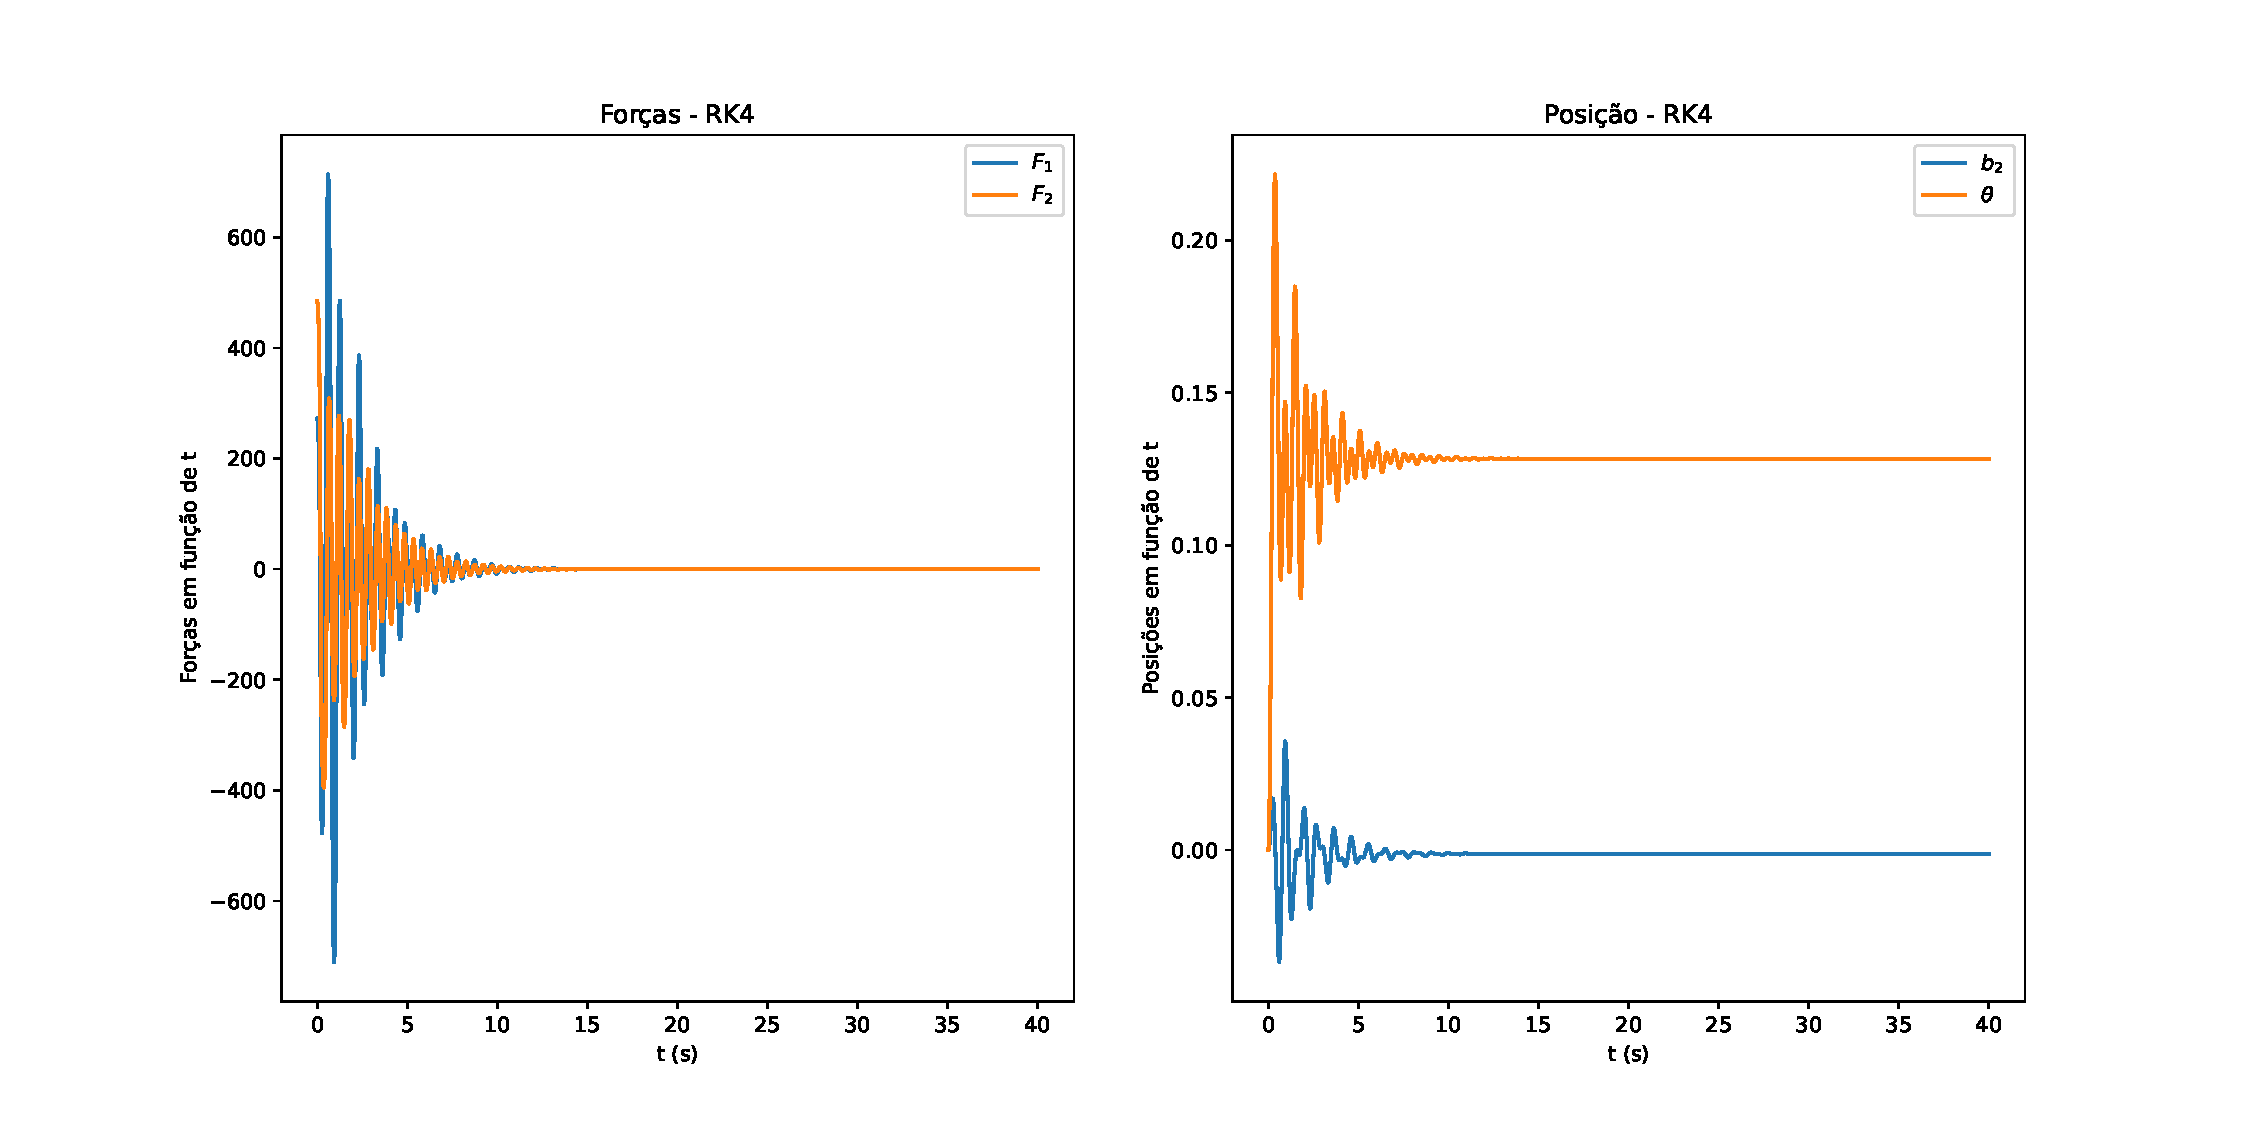
\includegraphics[width=\textwidth]{triangulo_retangulo/PVI_h=0.03_g1=500.0_g2=1.0.pdf}
            \caption{$\gamma_2 = 1.0$}
        \end{subfigure}
        \quad
        \begin{subfigure}[b]{0.9\textwidth}
            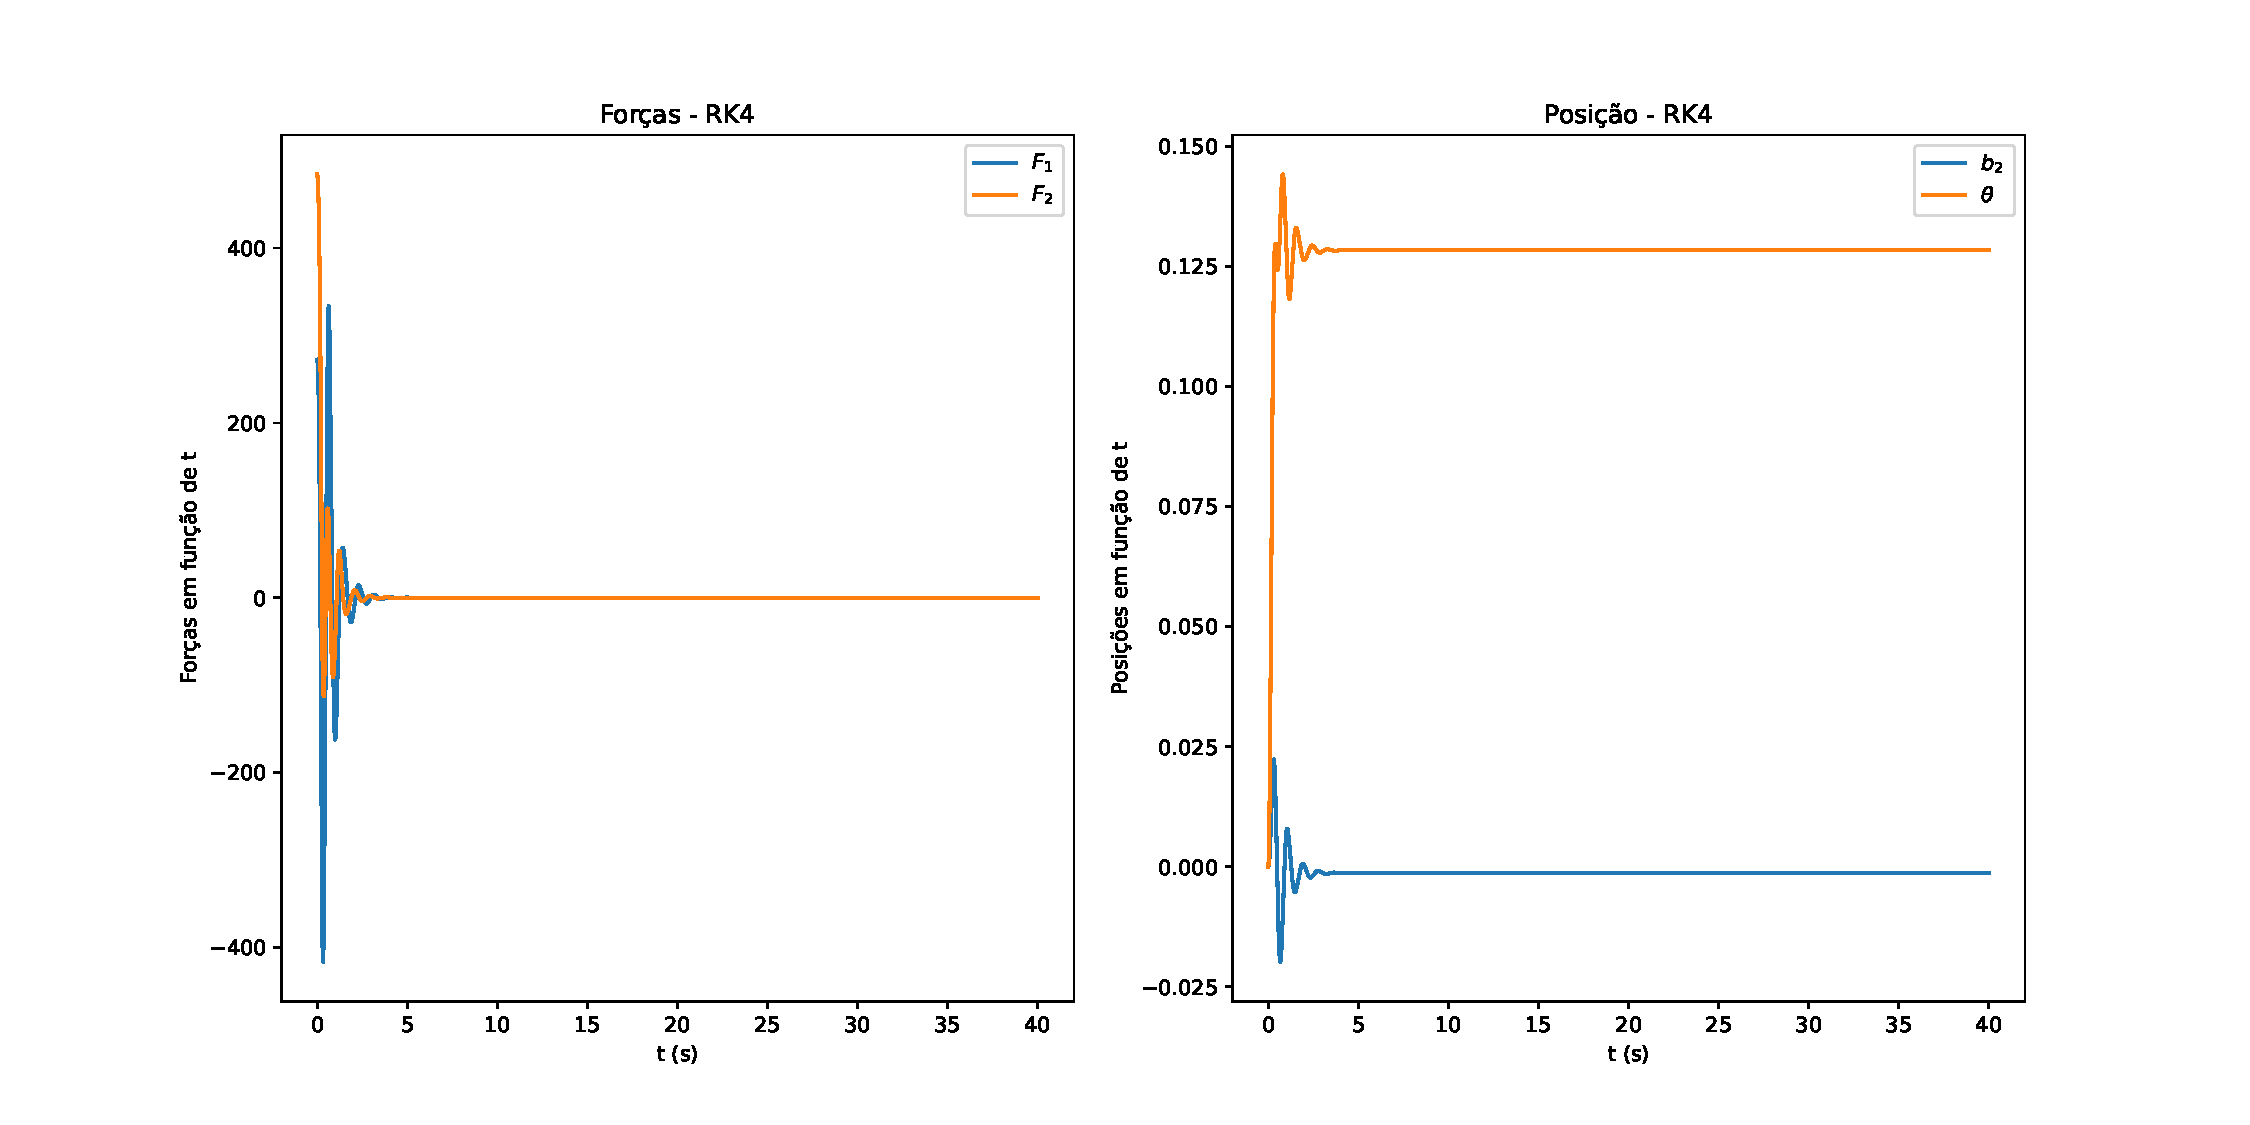
\includegraphics[width=\textwidth]{triangulo_retangulo/PVI_h=0.03_g1=500.0_g2=10.0.pdf}
            \caption{$\gamma_2 = 10.0$}
        \end{subfigure}
        \caption{PVI com $\gamma_1 = 500.0$ (Triângulo)}
        \label{fig:triang_PVI2}
    \end{figure}

    \begin{figure}
        \centering
        \begin{subfigure}[b]{0.9\textwidth}
            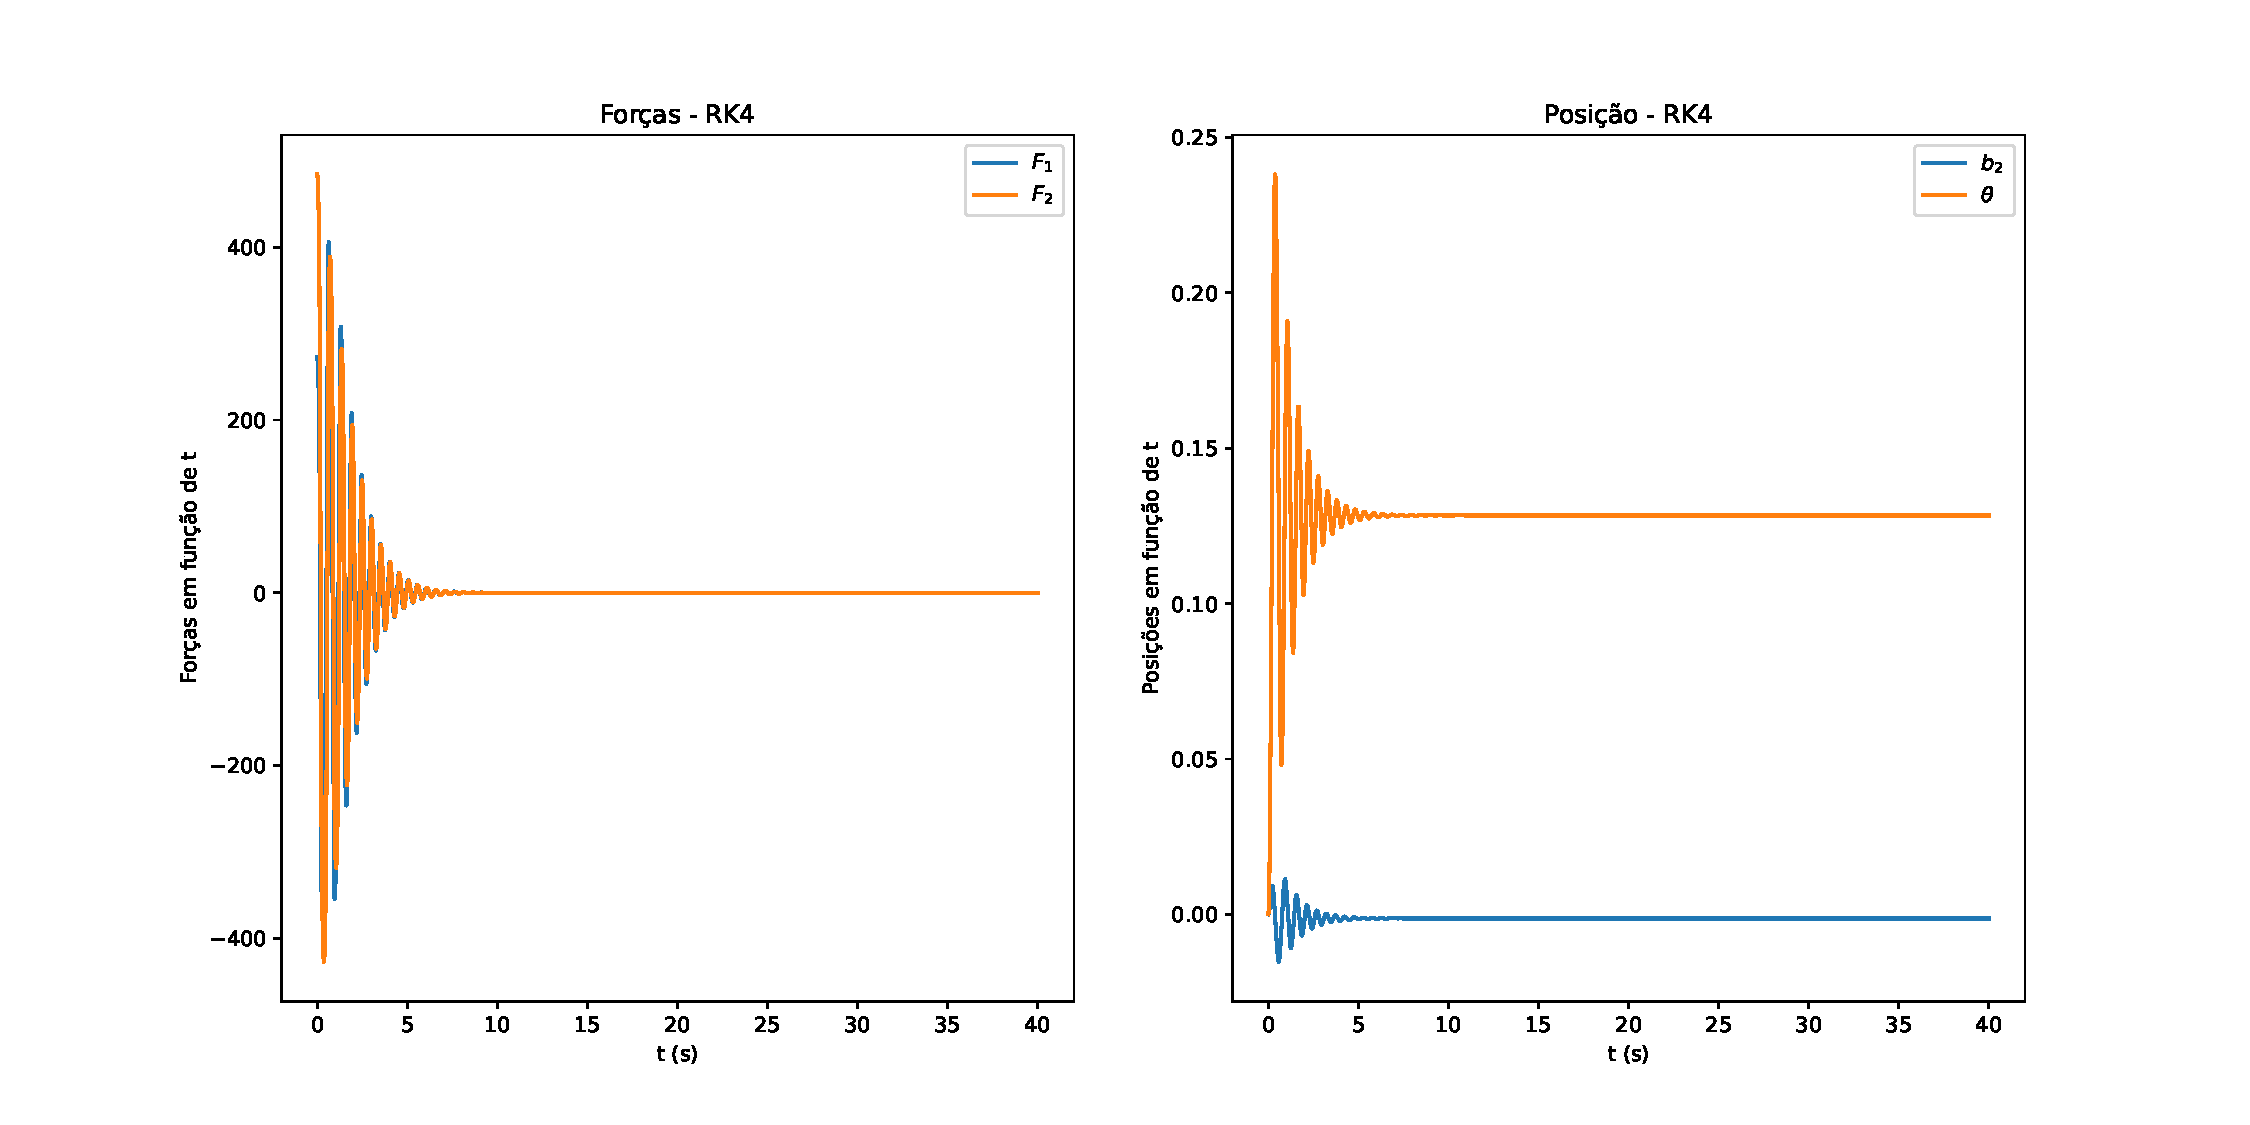
\includegraphics[width=\textwidth]{triangulo_retangulo/PVI_h=0.03_g1=5000.0_g2=0.5.pdf}
            \caption{$\gamma_2 = 0.5$}
        \end{subfigure}
        \quad
        \begin{subfigure}[b]{0.9\textwidth}
            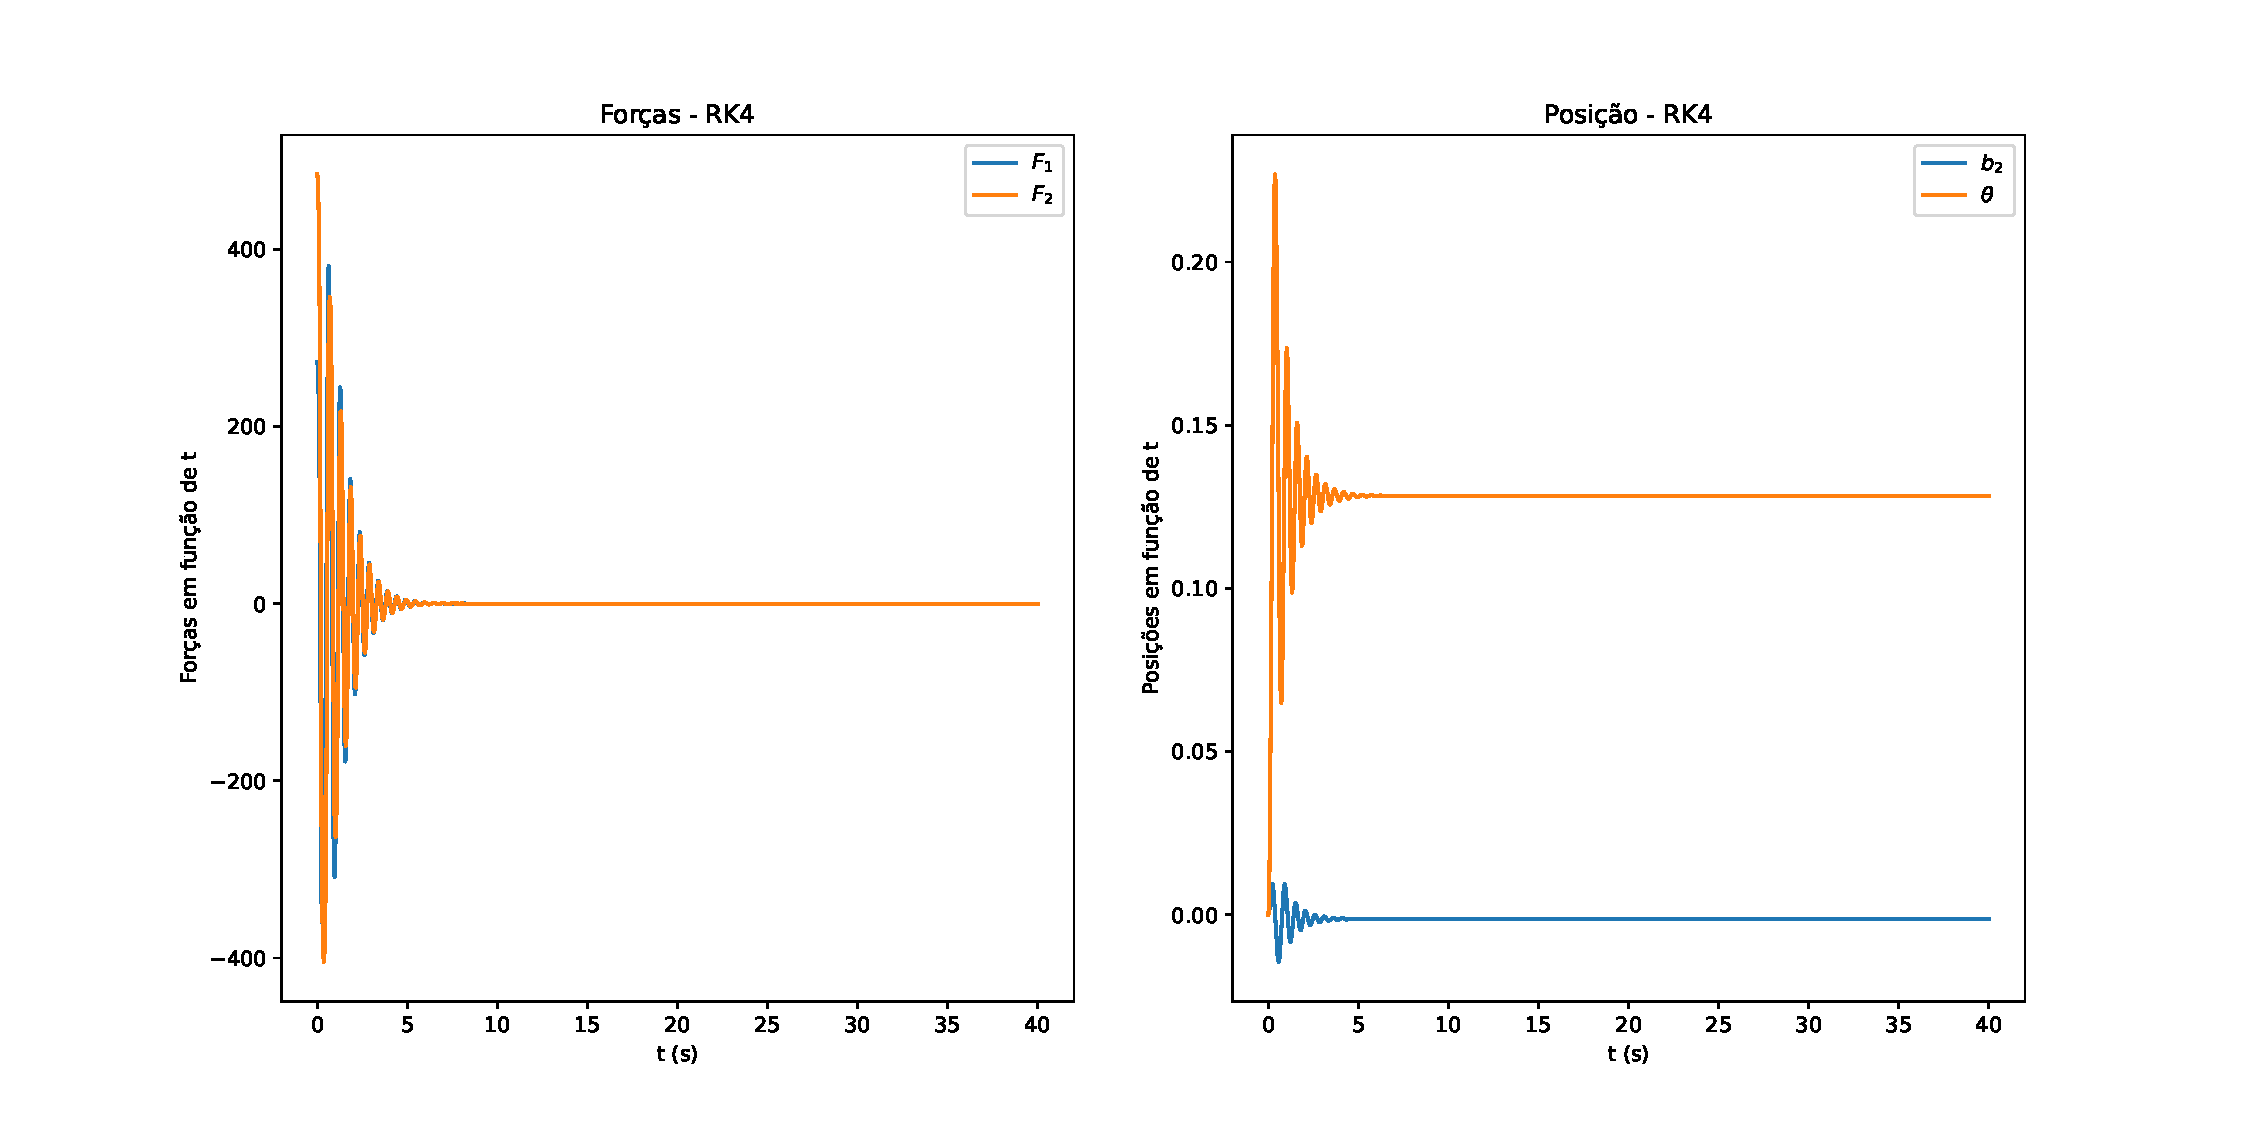
\includegraphics[width=\textwidth]{triangulo_retangulo/PVI_h=0.03_g1=5000.0_g2=1.0.pdf}
            \caption{$\gamma_2 = 1.0$}
        \end{subfigure}
        \quad
        \begin{subfigure}[b]{0.9\textwidth}
            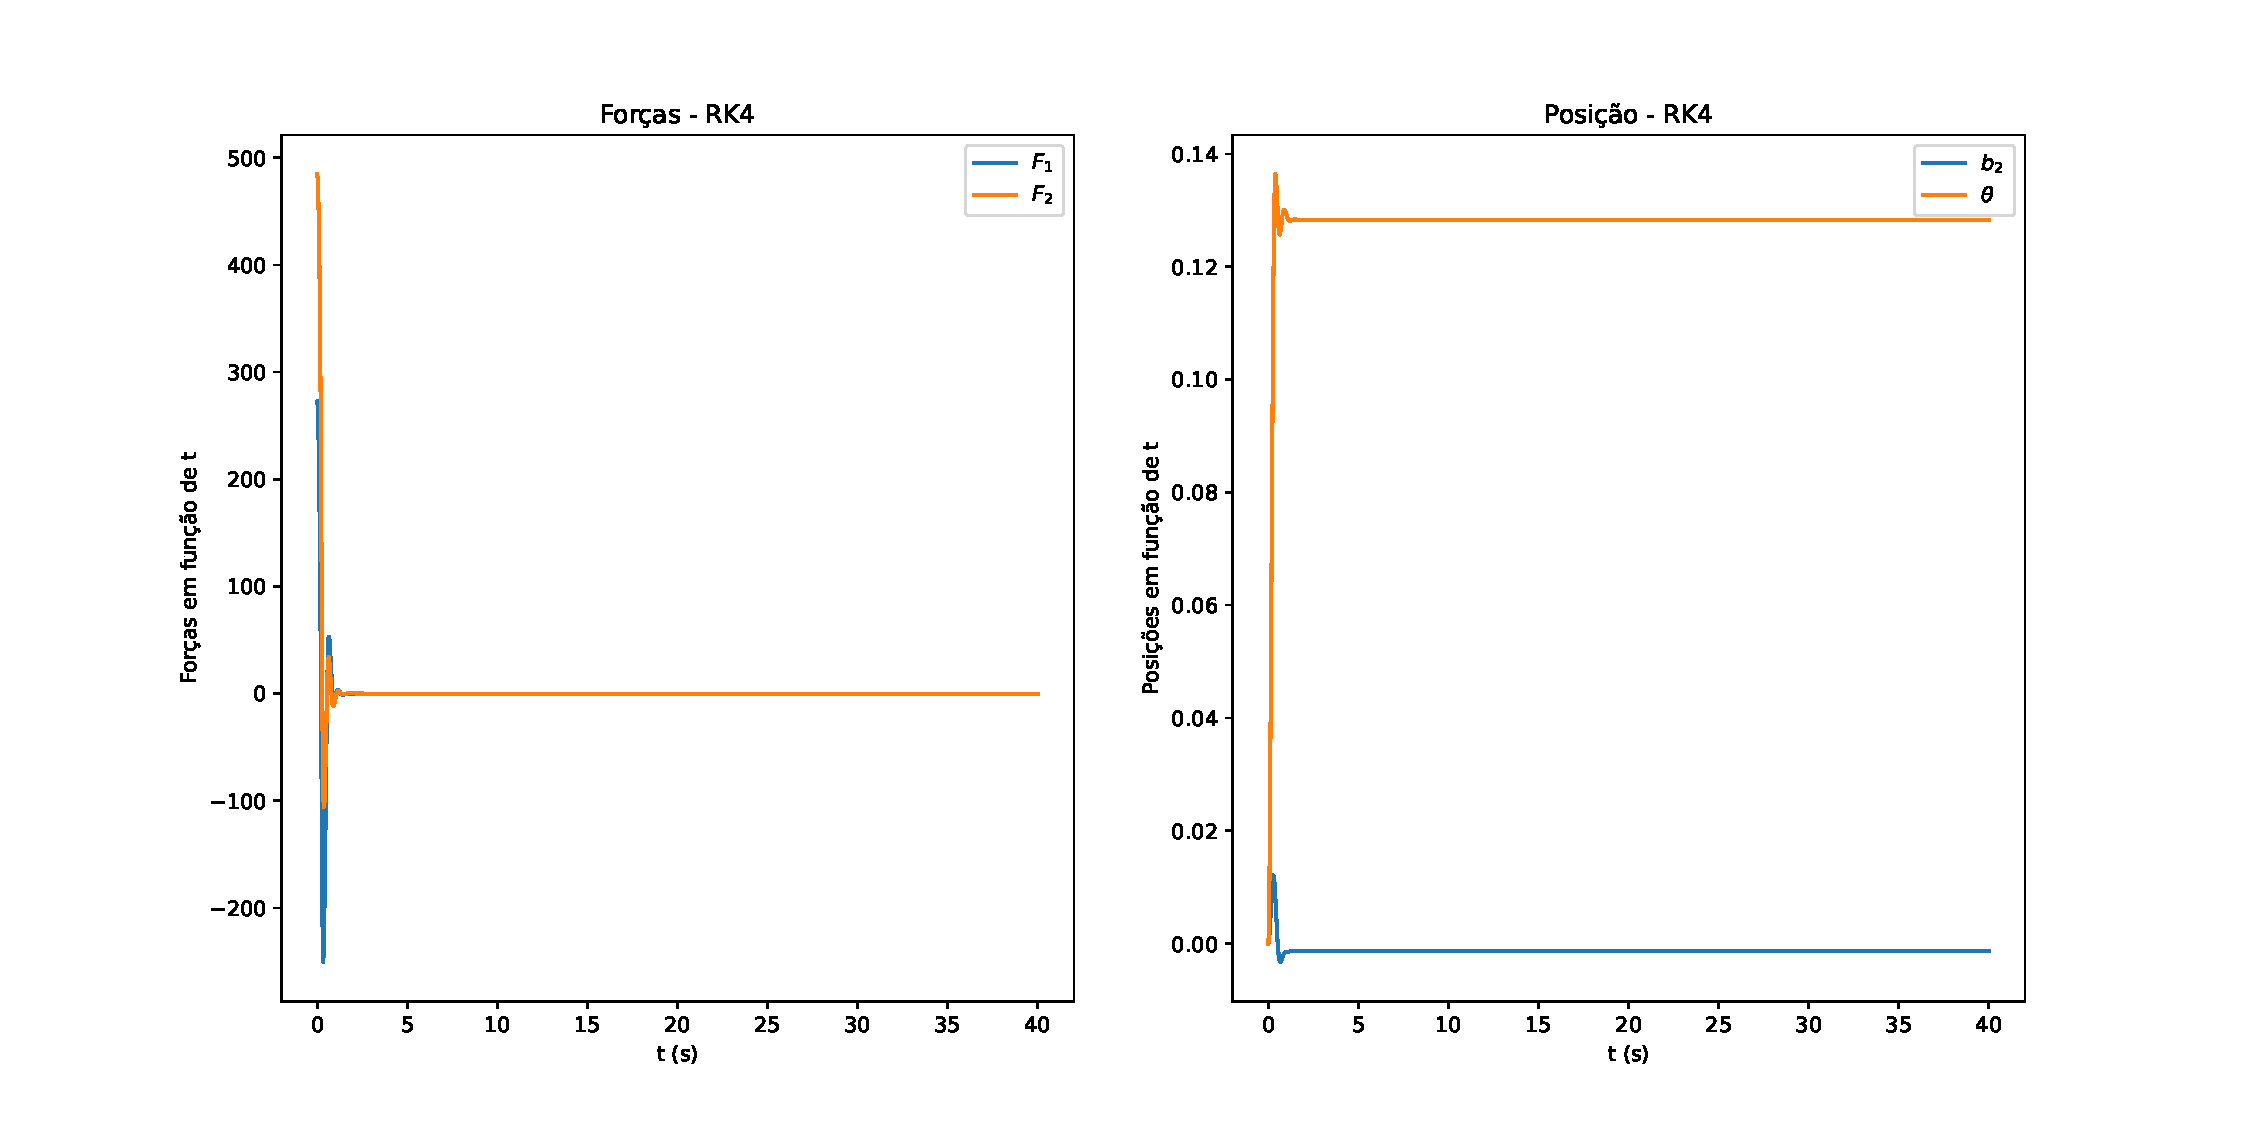
\includegraphics[width=\textwidth]{triangulo_retangulo/PVI_h=0.03_g1=5000.0_g2=10.0.pdf}
            \caption{$\gamma_2 = 10.0$}
        \end{subfigure}
        \caption{PVI com $\gamma_1 = 5000.0$ (Triângulo)}
        \label{fig:triang_PVI3}
    \end{figure}

    \begin{figure}[H]
        \centering
        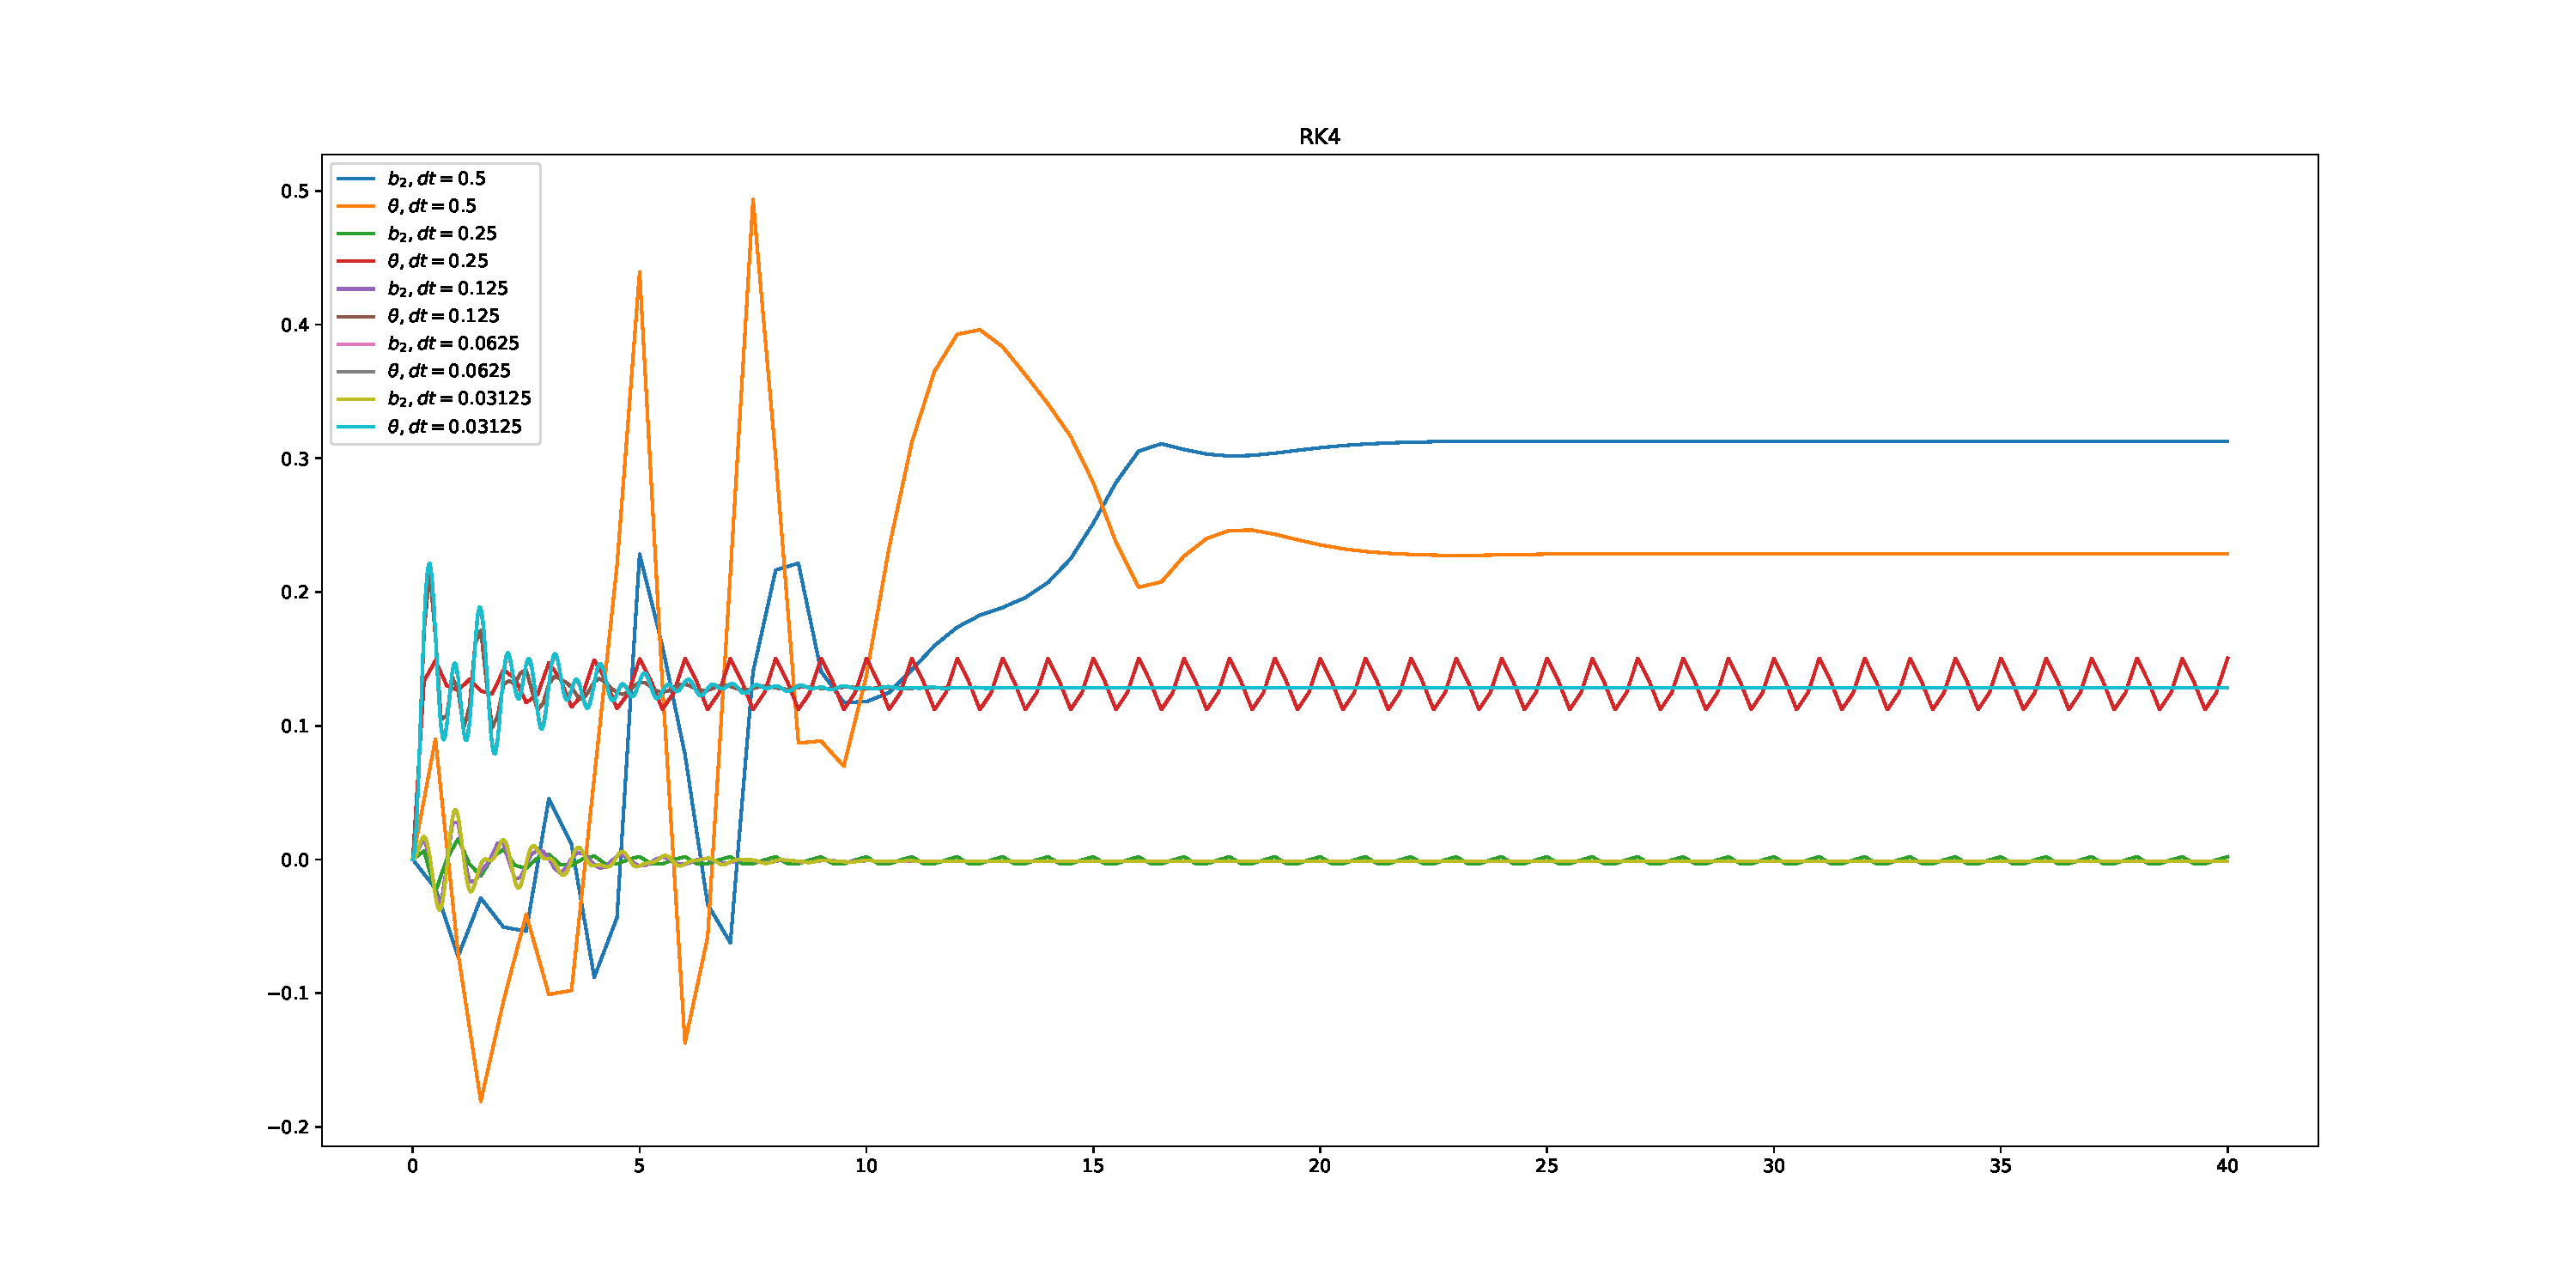
\includegraphics[width=\textwidth]{triangulo_retangulo/PVI_conv.pdf}
        \caption{$\theta$ e $b_2$ em função do tempo para diversos passos de tempo no caso do triângulo retângulo}
        \label{fig:triang_conv1}
    \end{figure}

    \begin{figure}[H]
        \centering
        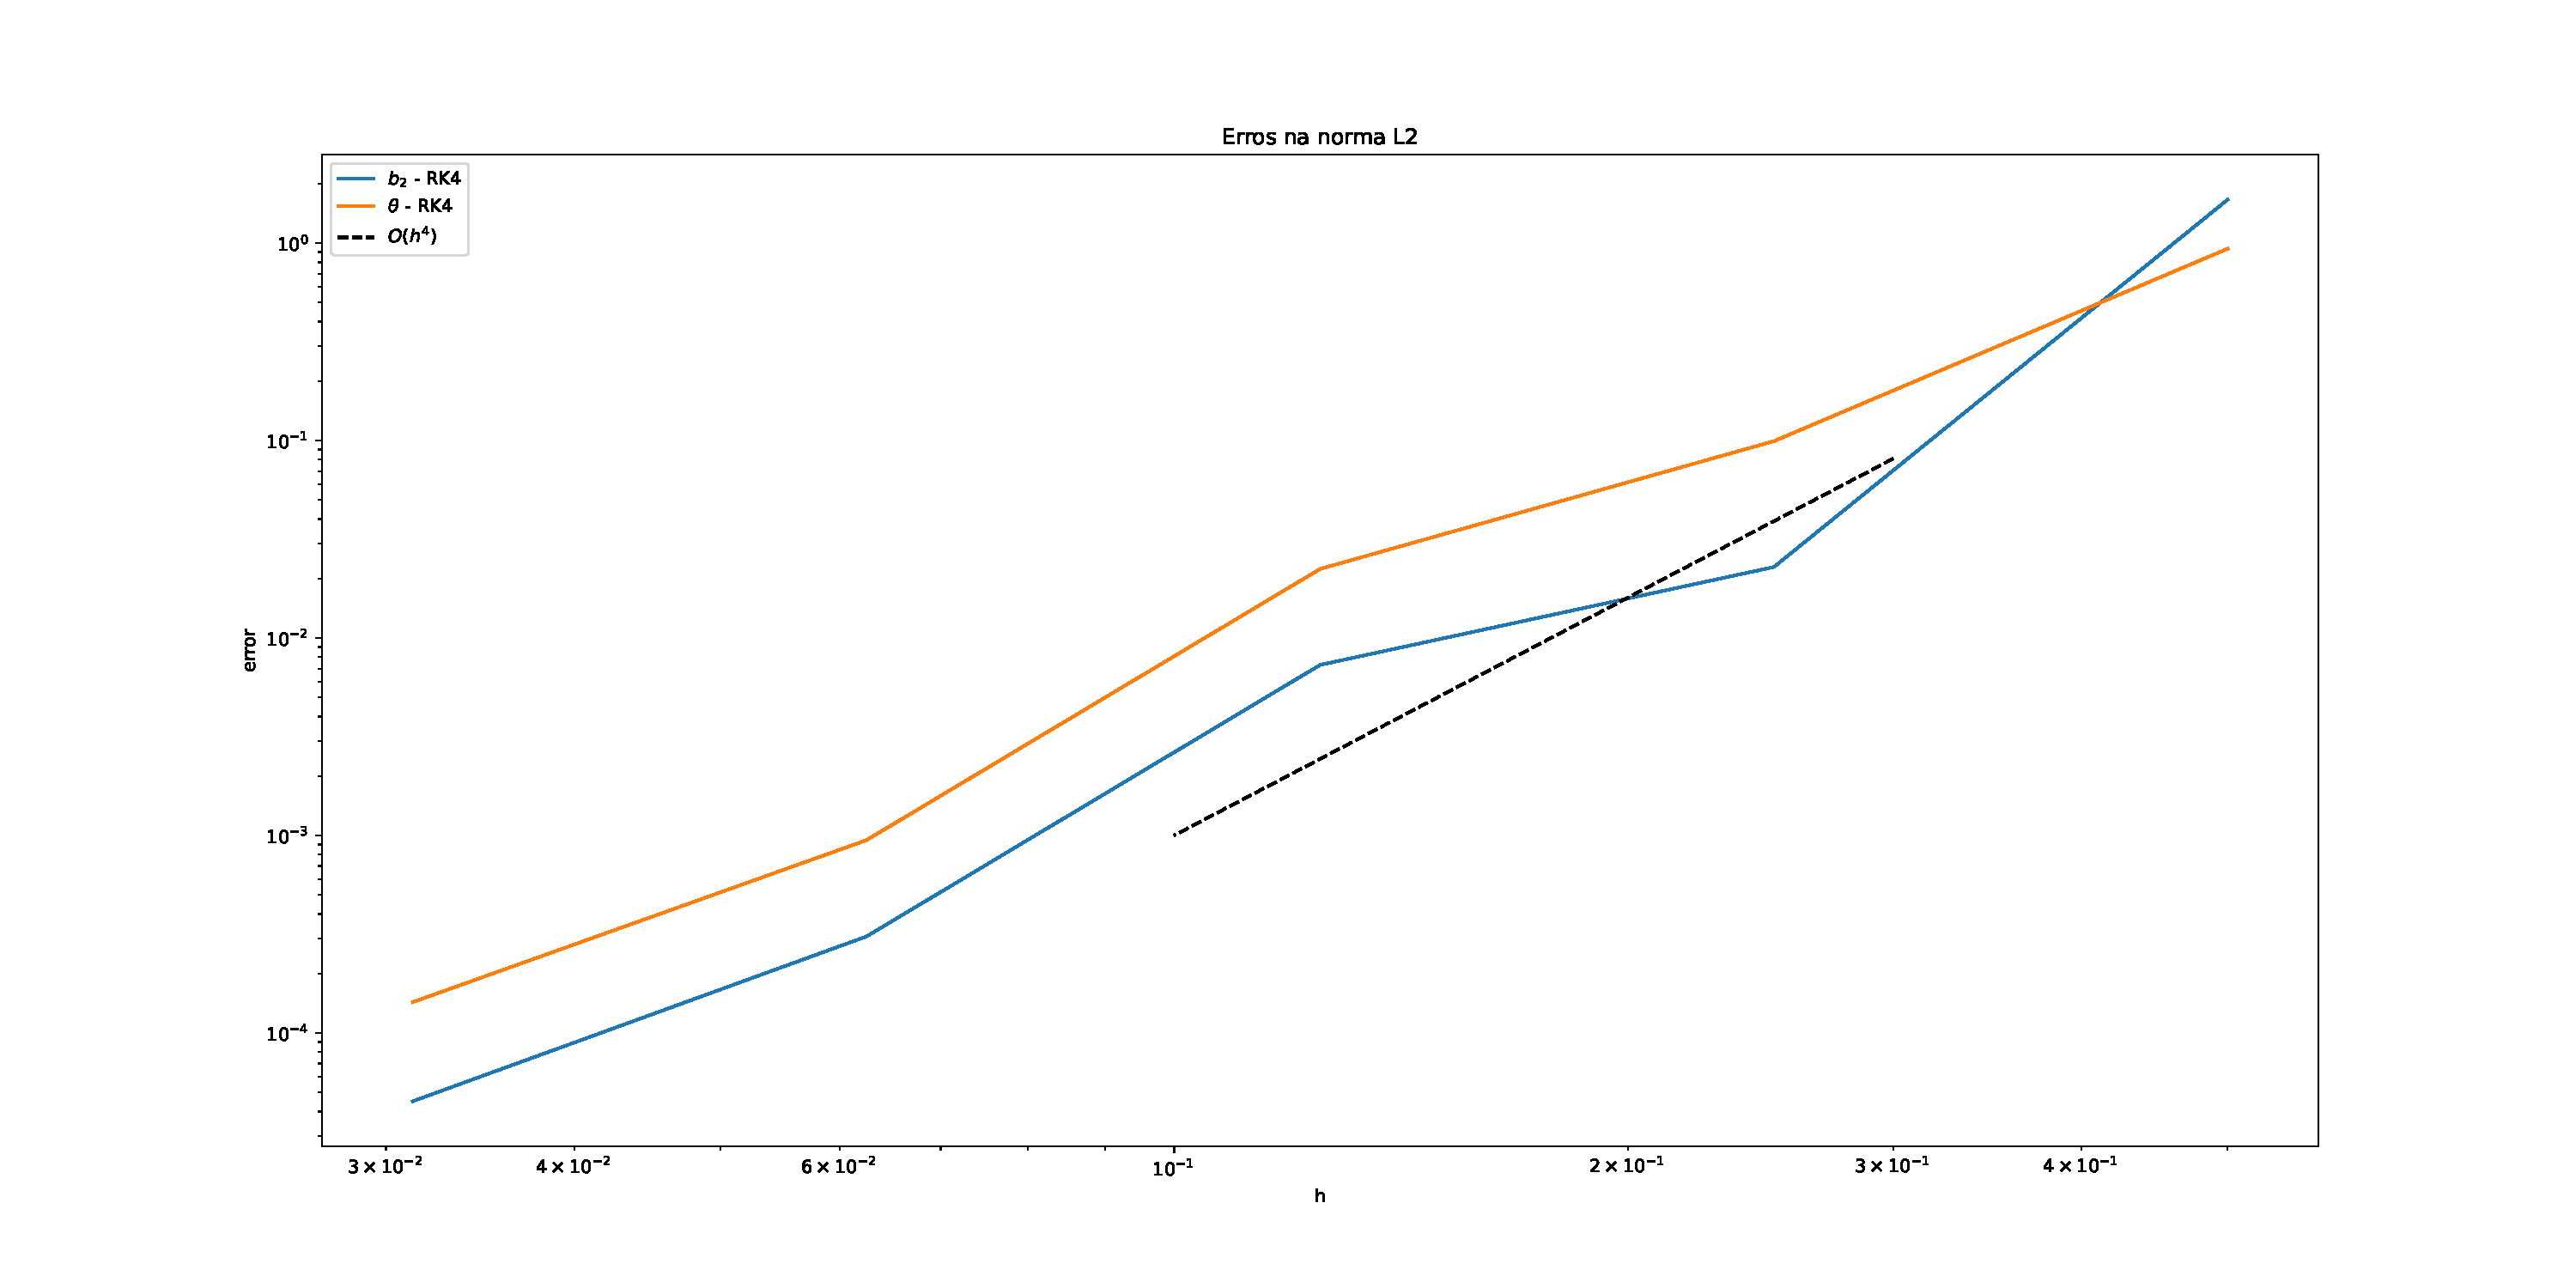
\includegraphics[width=\textwidth]{triangulo_retangulo/PVI_conv2.pdf}
        \caption{Ordem de convergência do método para solução do PVI (triângulo)}
        \label{fig:triang_conv2}
    \end{figure}

    \FloatBarrier


    \subsection{Equilíbrio e a geometria dos objetos}
    \label{sec:geo}
    É intuitivo que a geometria de um corpo dite que um ponto de equilíbrio seja estável ou instável, porém algumas características específicas parecem contribuir mais para isso. 
    
    \subsubsection{Pontas no corpo}
    Os dois objetos que possuíam estruturas semelhantes a cúspides, o iceberg e o triângulo, foram os que apresentaram comportamento dinâmico mais irregular. Uma possível explicação está na variação abrupta da geometria da fronteira nas proximidades dessas pontas. Durante uma pequena rotação ou translação, a região submersa pode mudar de maneira sensível, alterando a distribuição da pressão hidrostática e, consequentemente, o empuxo e o torque resultantes.

    Essa dependência geométrica pode tornar o campo de forças mais sensível à posição do corpo. Como o método de Newton utiliza uma aproximação numérica da matriz jacobiana, variações acentuadas das forças também podem prejudicar a qualidade dessa aproximação e reduzir a convergência observada. Isso é compatível com as ordens médias inferiores à quadrática obtidas para o triângulo e com a maior irregularidade observada nas trajetórias dinâmicas. Entretanto, os resultados apresentados não demonstram que as pontas sejam a única causa desse comportamento: a discretização da fronteira, a escolha do passo temporal e o acoplamento entre rotação e translação também podem contribuir.

    \subsubsection{Quais são os pontos de equilíbrio instável}
    A inspeção dos mapas de força sugere que os pontos 1 e 3 do iceberg e os pontos 1 e 3 do Titanic e do triângulo não podem ser classificados de forma conclusiva apenas pela visualização dos campos vetoriais. Já os pontos 1 e 3 do iceberg foram descritos como instáveis, enquanto os pontos 2 e 4 do Titanic e do triângulo apresentam comportamento compatível com instabilidade. Note que os equilíbrios estáveis, de maneira geral, ocorrem quando o maior eixo do objeto está mais alinhado à superfície do líquido.

    Quando um objeto está com o maior eixo perpendicular à superfície do líquido, sua massa está concentrada numa região horizontal pequena e, uma pequena rotação pode fazer com que o objeto tenha massa submersa em um lado do centro de massa, enquanto no outro a massa movida pela rotação estará acima do líquido. Isso acaba por gerar mais torque na direção em que o corpo já está girando, tornando o equilíbrio instável.

    Por outro lado, quando a massa está melhor distribuída horizontalmente, qualquer rotação acaba por deixar o corpo mais vertical. Isso faz com que o torque gerado seja na direção em que o corpo já está girando.

    \section{Conclusão}
    Neste trabalho, foi implementado um modelo bidimensional simplificado para estudar a flutuação de corpos rígidos sob ação da gravidade e da pressão hidrostática. A representação dos objetos por segmentos de reta permitiu reduzir o cálculo de grandezas geométricas e das forças a integrais de contorno, avaliadas numericamente por quadratura de Gauss--Legendre. As transformações rígidas foram tratadas por coordenadas homogêneas, enquanto as posições de equilíbrio foram calculadas pelo método de Newton--Raphson, com jacobiana aproximada por diferenças finitas. Para estudar o movimento transiente, o sistema foi reescrito como um problema de valor inicial e resolvido pelo método clássico de Runge--Kutta de quarta ordem.

    Os testes de consistência e de refinamento da representação poligonal indicaram que diversas grandezas geométricas convergem conforme o número de segmentos aumenta. Para o círculo, os erros apresentados nas tabelas diminuem aproximadamente por um fator de quatro a cada duplicação do número de segmentos, comportamento compatível com convergência de segunda ordem. A solução manufaturada também constitui uma verificação útil da implementação, encontrando erros nulos em todos os casos testados.

    A análise dos três objetos revelou múltiplas posições de equilíbrio e destacou a influência da geometria sobre o campo de forças. O Titanic, cuja forma é mais regular, apresentou mapas de força e trajetórias relativamente mais simples. O iceberg e o triângulo retângulo exibiram respostas mais irregulares, possivelmente relacionadas às pontas e à sensibilidade da região submersa a pequenas mudanças de posição. Em vários testes, a translação e a rotação mostraram forte acoplamento, de modo que a escolha dos coeficientes de amortecimento influenciou tanto as oscilações quanto o tempo necessário para a solução se aproximar de um estado estacionário.

    Os resultados também reforçam que a convergência do método de Newton não deve ser confundida com a estabilidade física do equilíbrio. A ordem estimada a partir das iterações variou entre os casos e pode ter sido afetada pela aproximação da jacobiana, pela tolerância e pela estimativa do erro em relação à última iteração. Para classificar a estabilidade com maior rigor, recomenda-se linearizar o sistema dinâmico em torno de cada equilíbrio e calcular os autovalores da matriz correspondente.

    \printbibliography
\end{document}
